
% main.tex
% ============================================
% 张芷芬等《微分方程定性理论》—— LaTeX 重排本
% 原著：张芷芬、丁同仁、黄文灶、董镇喜，微分方程定性理论
%       （科学出版社）
%
% 目的：将扫描版原书完整、忠实地逐页转为 LaTeX 排版。
% 编译：XeLaTeX + biber
% 模板参考：Arnold《常微分方程》笔记工程 的版式与定理环境体系
% ============================================
\documentclass{book}

% ── 加载所有配置 ──
% preamble/packages.tex
\usepackage{ctex}
\usepackage{lipsum}
\usepackage{amsmath, amsthm, amssymb, amsfonts, mathrsfs}
\usepackage{thmtools}
\usepackage{graphicx}
\usepackage{setspace}
\usepackage{geometry}
\usepackage{float}
\usepackage{hyperref}
\usepackage{framed}
\usepackage[dvipsnames]{xcolor}
\usepackage{tikz-cd}
\usepackage[most]{tcolorbox}
\tcbuselibrary{theorems}
\tcbuselibrary{breakable}
\usepackage{fontspec}
\usepackage{xeCJK}
\usepackage{listings}
\usetikzlibrary{matrix, arrows.meta}
\usepackage[style=ieee]{biblatex}
\usepackage{caption}
\usepackage{tikz}
\usetikzlibrary{arrows.meta, positioning}

% preamble/colors.tex
% ============================================
% 配色方案：绛紫 + 香槟金 (Deep Purple & Champagne Gold)
% 主色：绛紫 (Purple)  —— 章节彩带、定理框架
% 强调：香槟金 (Gold)   —— 定义、装饰线、点缀
% 辅助：淡紫 / 淡金     —— 辅助盒子、背景
% ============================================

% ---- 绛紫系（主结构色）----
\definecolor{PurpleDeep}{RGB}{45, 31, 54}      % #2D1F36 — 深绛紫
\definecolor{PurpleMain}{RGB}{59, 42, 69}      % #3B2A45 — 主绛紫
\definecolor{PurpleMed}{RGB}{91, 63, 102}      % #5B3F66 — 中绛紫
\definecolor{PurpleLight}{RGB}{139, 111, 149}  % #8B6F95 — 浅绛紫
\definecolor{PurplePale}{RGB}{240, 234, 240}   % #F0EAF0 — 淡紫

% ---- 香槟金系（强调色）----
\definecolor{GoldDeep}{RGB}{156, 123, 77}      % #9C7B4D
\definecolor{GoldMain}{RGB}{201, 168, 106}     % #C9A86A
\definecolor{GoldMed}{RGB}{223, 198, 148}      % #DFC694
\definecolor{GoldLight}{RGB}{234, 215, 178}    % #EAD7B2
\definecolor{GoldPale}{RGB}{245, 232, 208}     % #F5E8D0

% ---- 兼容别名（让 cover.tex、chapter.title.tex、part.title.tex 等无需改动）----
\colorlet{BlueMain}{PurpleMain}
\colorlet{BlueDark}{PurpleDeep}
\colorlet{BlueLight}{PurpleLight}
\colorlet{BlueMed}{PurpleMed}
\colorlet{BluePale}{PurplePale}

\colorlet{GreenMain}{PurpleMain}
\colorlet{GreenDark}{PurpleDeep}
\colorlet{GreenLight}{PurpleLight}
\colorlet{GreenMed}{PurpleMed}
\colorlet{GreenPale}{PurplePale}

\colorlet{VerdeMain}{GoldMain}
\colorlet{VerdeDark}{GoldDeep}
\colorlet{VerdeLight}{GoldLight}
\colorlet{VerdeMed}{GoldMed}
\colorlet{VerdePale}{GoldPale}

\colorlet{TealMain}{GoldMain!85!white}
\colorlet{TealDark}{GoldDeep}
\colorlet{TealLight}{GoldLight}
\colorlet{TealPale}{GoldPale!90!white}

\colorlet{LogicBlue}{PurpleMain}
\colorlet{LogicDarkBlue}{PurpleDeep}
\colorlet{LogicLightBlue}{PurpleLight}

\colorlet{GreenMainAlias}{PurpleMain}
\colorlet{OrangeMain}{PurpleMain!85}
\colorlet{SlateMain}{PurpleMain}
\colorlet{SlateMed}{PurpleMed}
\colorlet{SlateDark}{PurpleDeep}
\colorlet{SlateLight}{PurpleLight}

\colorlet{mainblue}{PurpleMain}
\colorlet{mediumblue}{PurpleDeep}
\colorlet{lightblue}{PurpleLight}
\colorlet{grayblue}{PurpleMain!50}
\colorlet{brightblue}{GoldMain}
\colorlet{paleblue}{PurpleMain!5}

\lstset{
	backgroundcolor=\color{PurpleMain!4},
	basicstyle=\ttfamily\small,
	keywordstyle=\color{PurpleMain},
	commentstyle=\color{PurpleMain!40},
	escapeinside={(*@}{@*)},
}
% preamble/theorems.tex
% ============================================
% 定理环境体系 —— 绛紫 + 香槟金
% 使用 \newtcbtheorem，每个环境接受 {标题}{标签} 两个参数
% 标题栏格式：环境名 + 编号 + "：" + 自定义小标题
%   调用示例：
%     \begin{theorem}{存在唯一性定理}{thm:exist}
%       设 $f$ 在区域 $G\subset\R\times\R^n$ 上连续且关于 $x$ 满足
%       Lipschitz 条件，则初值问题存在唯一解。
%     \end{theorem}
%     \begin{definition}{词项的定义}{def:term}
%       ……
%     \end{definition}
% ============================================

% ---- 全局正文定理样式：原书为无框、无色栏的行内标题 ----
\tcbset{
  qttheo/.style={
    breakable, enhanced, frame hidden, detach title,
    arc=0pt, boxrule=0pt, leftrule=0pt,
    fonttitle=\bfseries\theoremFont,
    fontupper=\theoremFont,
    colback=white, colbacktitle=white, coltitle=black,
    left=0pt, right=0pt, top=0pt, bottom=0pt,
    before skip=8pt, after skip=4pt,
    before upper={\tcbtitle\quad},
  }
}

% ---- 彩条标题格式：环境名 + 编号 + (有自定义标题时) "：" + 自定义标题 ----
\newcommand{\qttheotitle}[3]{%
  #1\ #2\IfBlankT{#3}{：#3}%
}

% ============================================================
% 类别 I — LogicBlue (绛紫主色)
% 定理 / 推论 / 命题 / 原理
% 编号采用章内计数（number within=chapter），与原书"定理 1.x"约定一致
% ============================================================
\newtcbtheorem[number within=section]{theorem}{定理}{
  qttheo,
  colback=white, colframe=LogicBlue,
  separator sign={},
  title={\qttheotitle{\thmt@thmname}{\thmt@thmnumber}{\thmt@tmptitle}},
}{thm}

\newtcbtheorem[use counter from=theorem]{corollary}{推论}{
  qttheo,
  colback=white, colframe=LogicBlue,
  separator sign={},
  title={\qttheotitle{\thmt@thmname}{\thmt@thmnumber}{\thmt@tmptitle}},
}{cor}

\newtcbtheorem[use counter from=theorem]{proposition}{命题}{
  qttheo,
  colback=white, colframe=LogicBlue,
  separator sign={},
  title={\qttheotitle{\thmt@thmname}{\thmt@thmnumber}{\thmt@tmptitle}},
}{prp}

\newtcbtheorem[use counter from=theorem]{prp}{原理}{
  qttheo,
  colback=white, colframe=LogicBlue,
  separator sign={},
  title={\qttheotitle{\thmt@thmname}{\thmt@thmnumber}{\thmt@tmptitle}},
}{prn}

% ============================================================
% 类别 II — LogicDarkBlue (深绛紫)
% 公理 / 问题 / 引理 / 注记
% ============================================================
\newtcbtheorem[use counter from=theorem]{axiom}{公理}{
  qttheo,
  colback=white, colframe=LogicDarkBlue,
  separator sign={},
  title={\qttheotitle{\thmt@thmname}{\thmt@thmnumber}{\thmt@tmptitle}},
}{ax}

\newtcbtheorem[use counter from=theorem]{problem}{问题}{
  qttheo,
  colback=white, colframe=LogicDarkBlue,
  separator sign={},
  title={\qttheotitle{\thmt@thmname}{\thmt@thmnumber}{\thmt@tmptitle}},
}{pb}

\newtcbtheorem[use counter from=theorem]{lemma}{引理}{
  qttheo,
  colback=white, colframe=LogicDarkBlue,
  separator sign={},
  title={\qttheotitle{\thmt@thmname}{\thmt@thmnumber}{\thmt@tmptitle}},
}{lem}

\newtcbtheorem[use counter from=theorem]{remark}{注记}{
  qttheo,
  colback=white, colframe=LogicDarkBlue,
  separator sign={},
  title={\qttheotitle{\thmt@thmname}{\thmt@thmnumber}{\thmt@tmptitle}},
}{rem}

% ============================================================
% 类别 III — GoldMain (香槟金)
% 定义 —— 金色边框 + 淡紫底 + 深紫标题文字
% ============================================================
\newtcbtheorem[use counter from=theorem]{definition}{定义}{
  qttheo,
  colback=PurplePale, colframe=GoldMain,
  fonttitle=\bfseries\theoremFont\color{PurpleDeep},
  separator sign={},
  title={\qttheotitle{\thmt@thmname}{\thmt@thmnumber}{\thmt@tmptitle}},
}{def}

% ============================================================
% 类别 IV — LogicLightBlue (浅绛紫)
% 构造 / 记号 / 说明
% ============================================================
\newtcbtheorem[use counter from=theorem]{construction}{构造}{
  qttheo,
  colback=white, colframe=LogicLightBlue,
  separator sign={},
  title={\qttheotitle{\thmt@thmname}{\thmt@thmnumber}{\thmt@tmptitle}},
}{con}

\newtcbtheorem[use counter from=theorem]{note}{记号}{
  qttheo,
  colback=white, colframe=LogicLightBlue,
  separator sign={},
  title={\qttheotitle{\thmt@thmname}{\thmt@thmnumber}{\thmt@tmptitle}},
}{no}

\newtcbtheorem[use counter from=theorem]{ill}{说明}{
  qttheo,
  colback=white, colframe=LogicLightBlue,
  separator sign={},
  title={\qttheotitle{\thmt@thmname}{\thmt@thmnumber}{\thmt@tmptitle}},
}{il}

% ============================================================
% 类别 V
% 示例 —— 无框正文，按节独立连续编号
% 调用方式仍为 \begin{example}{标题}{标签} ... \end{example}
% ============================================================
\newcounter{example}[section]
\renewcommand{\theexample}{\thesection.\arabic{example}}

\NewDocumentEnvironment{example}{m m}{%
  \par\medskip
  \refstepcounter{example}%
  \ifstrempty{#2}{}{\label{ex:#2}}%
  \noindent{\bfseries\theoremFont
    示例~\theexample\ifstrempty{#1}{}{：#1}}\quad
  \theoremFont
}{%
  \par\medskip
}

% ============================================================
%  解 (Solution) 环境（无编号）
% ============================================================
\newcounter{solution}
\renewcommand{\thesolution}{\arabic{solution}}
\NewDocumentEnvironment{solution}{}{%
  \par\proofFont
  \refstepcounter{solution}%
  \noindent\textbf{解.}\quad
}{%
  \hfill $\square$\par
}

% ============================================================
%  证明 (Proof) 环境（可自定义小标题，如 证明（充分性））
%  amsthm 已定义 proof，此处用标准语法重定义
% ============================================================
\renewenvironment{proof}[1][证明]{%
  \par\proofFont
  \noindent\textbf{#1}\quad
}{%
  \par
}

% ---- 行距 ----
\setstretch{1.2}

% ============================================================
%  附注 / 命名定理 / 命名引理（无编号，行内加粗，仿原书）
%  用于 附注 1/2/3、Cauchy-Peano 定理、Gronwall 引理 等
% ============================================================
\newcommand{\fuzhu}[2]{\par\medskip\noindent\textbf{附注~#1}\quad #2\par\medskip}
\newcommand{\namedthm}[2]{\par\medskip\noindent\textbf{#1~定理}\quad #2\par\medskip}
\newcommand{\namedlem}[2]{\par\medskip\noindent\textbf{#1~引理}\quad #2\par\medskip}
\newcommand{\namedcor}[2]{\par\medskip\noindent\textbf{推论~#1}\quad #2\par\medskip}

% preamble/commands.tex
% ============================================
% 自定义命令 —— 通用数学 + ODE 专用
% ============================================

% ---- 颜色文字命令 ----
\newcommand{\red}[1]{\textcolor[rgb]{1.00,0.00,0.00}{#1}}
\newcommand{\blue}[1]{\textcolor[rgb]{0.00,0.00,1.00}{#1}}
\newcommand{\green}[1]{\textcolor[rgb]{0.00,1.00,0.00}{#1}}
\newcommand{\darkblue}[1]{\textcolor[rgb]{0.00,0.00,0.50}{#1}}
\newcommand{\darkgreen}[1]{\textcolor[rgb]{0.00,0.37,0.00}{#1}}
\newcommand{\darkred}[1]{\textcolor[rgb]{0.60,0.00,0.00}{#1}}
\newcommand{\brown}[1]{\textcolor[rgb]{0.50,0.30,0.00}{#1}}
\newcommand{\purple}[1]{\textcolor[rgb]{0.50,0.00,0.50}{#1}}

% ---- 数学黑板体快捷命令 ----
\newcommand{\R}{\mathbb{R}}
\newcommand{\C}{\mathbb{C}}
\newcommand{\Z}{\mathbb{Z}}
\newcommand{\N}{\mathbb{N}}
\newcommand{\Q}{\mathbb{Q}}
\newcommand{\E}{\mathbb{E}}
\newcommand{\F}{\mathbb{F}}

% ---- 数学格式命令 ----
\newcommand{\dd}{\mathrm{d}}
\newcommand{\eps}{\varepsilon}
\newcommand{\abs}[1]{\left| #1 \right|}
\newcommand{\norm}[1]{\left\| #1 \right\|}
\newcommand{\bkt}[1]{\left\langle #1 \right\rangle}
\newcommand{\dif}{\mathop{}\!\mathrm{d}}
\newcommand{\parder}[2]{\frac{\partial #1}{\partial #2}}

% ---- 向量命令 ----
\newcommand{\vect}[1]{\boldsymbol{#1}}
\newcommand{\x}{\boldsymbol{x}}
\newcommand{\y}{\boldsymbol{y}}
\newcommand{\z}{\boldsymbol{z}}
\newcommand{\mat}[1]{\mathbf{#1}}

% ---- ODE 专用命令 ----
\newcommand{\ODE}{\,\mathrm{ODE}}
\newcommand{\IVP}{\,\mathrm{IVP}}
\newcommand{\BVP}{\,\mathrm{BVP}}
\newcommand{\dotx}{\dot{x}}
\newcommand{\doty}{\dot{y}}
\newcommand{\ddx}{\frac{\dd}{\dd t}}
\newcommand{\ddxx}{\frac{\dd^2}{\dd t^2}}
\newcommand{\dxdt}{\frac{\dd x}{\dd t}}
\newcommand{\dydt}{\frac{\dd y}{\dd t}}
\newcommand{\Lip}{\mathrm{Lip}}

% 相空间
\newcommand{\phase}{\Omega}

% 解算子 / 流
\newcommand{\flow}{\Phi}

% Jacobi 矩阵
\newcommand{\Jac}{\mathrm{D}}
\newcommand{\jac}[1]{\Jac #1}

% ---- 花体/手写体 ----
\newcommand{\T}{\mathcal{T}}
\newcommand{\X}{\mathrm{X}}
\newcommand{\Y}{\mathrm{Y}}
\newcommand{\B}{\mathcal{B}}

% ---- Arnold 风格附加命令 ----
% 向量场
\newcommand{\Vect}{\operatorname{Vect}}
% 微分同胚群
\newcommand{\Diff}{\operatorname{Diff}}
% 切空间 / 切丛
\newcommand{\tangent}{T}
\newcommand{\tangentbundle}{\mathrm{T}}
% Lie 导数
\newcommand{\Lieder}{\mathcal{L}}
% 指数映射
\newcommand{\Expmap}{\exp}
% 单参数群
\newcommand{\oneparam}{g}
% 首次积分
\newcommand{\firstint}{F}

% preamble/geometry.tex
% ============================================
% 页面布局 + 字体设置
% ============================================

% ---- 页面边距 ----
\geometry{
	textheight=9in,
	textwidth=5.5in,
	top=1in,
	headheight=12pt,
	headsep=25pt,
	footskip=30pt
}

% ---- 全局正文字体（英文 + 中文）----
\setmainfont{Times New Roman}
\setCJKmainfont{SimSun}
\setCJKmainfont{SimSun}[AutoFakeBold={3}]

% ---- 定理环境中文字体：仿宋 ----
\setCJKfamilyfont{theoremCJK}{FangSong}[AutoFakeBold={2.5}]
\newcommand{\theoremFont}{\CJKfamily{theoremCJK}}

% ---- 证明环境中文字体：楷体 ----
\setCJKfamilyfont{proofCJK}{KaiTi}[AutoFakeBold={2.5}]
\newcommand{\proofFont}{\CJKfamily{proofCJK}}

% preamble/chapter.title.tex
% 章节扉页设计 —— 墨绿 + 暗金
%   1. 上部图片从页面左边缘铺到右边缘
%   2. 章节名称位于横贯整页的彩条中
%   3. 彩条下方预留章节介绍区域
% =========================================================

\RequirePackage{tikz}
\RequirePackage{graphicx}
\RequirePackage{etoolbox}
\RequirePackage{setspace}

\makeatletter

% -------- 每章图片接口 --------
\newcommand{\chapterimage}{}
\newcommand{\setchapterimage}[1]{\gdef\chapterimage{#1}}

% -------- 章节介绍接口 --------
\newcommand{\chapterintro}{}
\newcommand{\setchapterintro}[1]{\gdef\chapterintro{#1}}

% -------- 版式参数 --------
\newlength{\ChapterTopImageHeight}
\setlength{\ChapterTopImageHeight}{14.2cm}

\newlength{\ChapterRibbonHeight}
\setlength{\ChapterRibbonHeight}{2.35cm}

\newlength{\ChapterIntroTopSep}
\setlength{\ChapterIntroTopSep}{1.15cm}

\newlength{\ChapterIntroWidth}
\setlength{\ChapterIntroWidth}{\dimexpr\textwidth+0.6cm\relax}

\newlength{\ChapterIntroLeft}
\setlength{\ChapterIntroLeft}{\dimexpr\paperwidth/2-\ChapterIntroWidth/2\relax}

\newlength{\ChapterImageMid}
\setlength{\ChapterImageMid}{\dimexpr\ChapterTopImageHeight/2\relax}

\newlength{\ChapterImageShadeTop}
\setlength{\ChapterImageShadeTop}{\dimexpr\ChapterTopImageHeight-1.0cm\relax}

\newlength{\ChapterRibbonMid}
\setlength{\ChapterRibbonMid}{\dimexpr\ChapterTopImageHeight+\ChapterRibbonHeight/2\relax}

\newlength{\ChapterRibbonBottom}
\setlength{\ChapterRibbonBottom}{\dimexpr\ChapterTopImageHeight+\ChapterRibbonHeight\relax}

\newlength{\ChapterIntroTop}
\setlength{\ChapterIntroTop}{\dimexpr\ChapterTopImageHeight+\ChapterRibbonHeight+\ChapterIntroTopSep\relax}

\newcommand{\ChapterIntroBlock}{%
	\ifdefempty{\chapterintro}{%
		\vspace*{6.4cm}%
	}{%
		{\Large\bfseries\color{GreenMain} 本章导读\par}%
		\vspace{0.55cm}%
		{\setstretch{1.35}\large\itshape\color{GreenMed}\chapterintro\par}%
	}%
}

\newcommand{\ChapterTitlePage}[1]{%
	\thispagestyle{empty}%
	\vspace*{-\baselineskip}%
	\begin{tikzpicture}[remember picture,overlay]
		\ifdefempty{\chapterimage}{%
			\shade[top color=GreenMain!18,bottom color=GreenMain!6]
				(current page.north west) rectangle
				([yshift=-\ChapterTopImageHeight]current page.north east);
			\node[align=center,text=GreenMed,font=\large\itshape]
				at ([yshift=-\ChapterImageMid]current page.north)
				{请在本章前设置章节图片};
		}{%
			\node[anchor=north west,inner sep=0pt,outer sep=0pt]
				at (current page.north west)
				{\includegraphics[
					width=\paperwidth,
					height=\ChapterTopImageHeight
				]{\chapterimage}};
		}%
		\shade[top color=black!0,bottom color=black!22]
			([yshift=-\ChapterImageShadeTop]current page.north west) rectangle
			([yshift=-\ChapterTopImageHeight]current page.north east);
		
		\fill[GreenMain!94]
			([yshift=-\ChapterTopImageHeight]current page.north west) rectangle
			([yshift=-\ChapterRibbonBottom]current page.north east);
		\fill[GoldMain!75]
			([yshift=-\ChapterTopImageHeight]current page.north west) rectangle
			([xshift=0.18cm,yshift=-\ChapterRibbonBottom]current page.north west);
		\fill[GoldMain!75]
			([xshift=-0.18cm,yshift=-\ChapterTopImageHeight]current page.north east) rectangle
			([yshift=-\ChapterRibbonBottom]current page.north east);
		\node[text=white,font=\bfseries\huge,align=center,text width=\dimexpr\paperwidth-2.2cm\relax]
			at ([yshift=-\ChapterRibbonMid]current page.north)
			{#1};
		\draw[GoldMain!45,line width=0.7pt]
			([yshift=-\ChapterRibbonBottom]current page.north west) --
			([yshift=-\ChapterRibbonBottom]current page.north east);
		
		\coordinate (introNW) at
			([xshift=\ChapterIntroLeft,
			  yshift=-\ChapterIntroTop]
			 current page.north west);
		\draw[GoldMain!45,line width=0.8pt] (introNW) -- ++(\ChapterIntroWidth,0);
		\node[anchor=north west,inner sep=0pt,outer sep=0pt,text width=\ChapterIntroWidth,align=left]
			at ([yshift=-0.55cm]introNW)
			{\ChapterIntroBlock};
	\end{tikzpicture}%
	\vspace*{\fill}%
	\clearpage%
}

\def\@makechapterhead#1{%
	\if@mainmatter
		\ChapterTitlePage{第\thechapter 章\quad #1}%
	\else
		\vspace*{50pt}%
		{\noindent\huge\bfseries #1\par}%
		\vskip 40pt%
	\fi
}

\def\@makeschapterhead#1{%
	\if@mainmatter
		\ChapterTitlePage{#1}%
	\else
		\vspace*{50pt}%
		{\noindent\huge\bfseries #1\par}%
		\vskip 40pt%
	\fi
}

\makeatother

% preamble/part.title.tex
% Part 扉页设计 —— 墨绿 + 暗金
% Arnold 的常微分方程原书未分 Part，此文件保留以备扩展使用。
% =========================================================

\RequirePackage{tikz}
\RequirePackage{graphicx}
\RequirePackage{etoolbox}
\RequirePackage{setspace}

\makeatletter

\gdef\partimage{}
\newcommand{\setpartimage}[1]{\gdef\partimage{#1}}

\gdef\partintro{}
\newcommand{\setpartintro}[1]{\gdef\partintro{#1}}

\newlength{\PartRibbonHeight}
\setlength{\PartRibbonHeight}{2.35cm}

\newlength{\PartContentTop}
\setlength{\PartContentTop}{\dimexpr\PartRibbonHeight+1.2cm\relax}

\newlength{\PartDividerY}
\setlength{\PartDividerY}{\dimexpr\PartRibbonHeight+6.8cm\relax}

\newcommand{\PartTitleBlock}[2]{%
    \ifdefempty{#1}{%
        \fill[GoldMain!55]
            ([xshift=1.8cm,yshift=-\PartContentTop]current page.north west)
            -- ++(0.22,0.22) -- ++(-0.22,0.22) -- ++(-0.22,-0.22) -- cycle;
    }{%
        \node[anchor=north west,text=GoldMain!72,font=\fontsize{52}{62}\bfseries]
            at ([xshift=1.8cm,yshift=-\PartContentTop]current page.north west)
            {#1};
        \node[anchor=north west,text=GoldMain!48,font=\Large\bfseries]
            at ([xshift=1.8cm,yshift=-\PartContentTop-3.1cm]current page.north west)
            {Part};
    }%
    \node[anchor=north west,text=BlueDark,font=\fontsize{22}{28}\bfseries,
          text width=8cm,align=left]
        at ([xshift=1.8cm,yshift=-\PartContentTop-4.4cm]current page.north west)
        {#2};
}

\newcommand{\PartIntroBlock}{%
    \ifdefempty{\partintro}{}{%
        \node[anchor=north east,text=BlueMain!80,font=\Large\bfseries]
            at ([xshift=-1.8cm,yshift=-\PartContentTop]current page.north east)
            {简\quad 介};
        \node[anchor=north east,text=BlueDark!55,font=\large\itshape,
              text width=7.4cm,align=right,inner sep=0pt]
            at ([xshift=-1.8cm,yshift=-\PartContentTop-1.5cm]current page.north east)
            {\setstretch{1.45}\partintro};
    }%
}

\newcommand{\PartTitlePage}[2]{%
    \thispagestyle{empty}%
    \vspace*{-\baselineskip}%
    \begin{tikzpicture}[remember picture,overlay]
        \fill[BlueMain!94]
            (current page.north west) rectangle
            ([yshift=-\PartRibbonHeight]current page.north east);
        \fill[GoldMain!75]
            (current page.north west) rectangle
            ([xshift=0.18cm,yshift=-\PartRibbonHeight]current page.north west);
        \fill[GoldMain!75]
            ([xshift=-0.18cm]current page.north east) rectangle
            ([yshift=-\PartRibbonHeight]current page.north east);
        \PartTitleBlock{#1}{#2}
        \PartIntroBlock
        \draw[GoldMain!20,line width=0.5pt,dash pattern=on 3pt off 5pt]
            ([xshift=11.0cm,yshift=-\PartContentTop]current page.north west) --
            ([xshift=11.0cm,yshift=-\PartDividerY+0.3cm]current page.north west);
        \draw[GoldMain!42,line width=0.7pt]
            ([yshift=-\PartDividerY]current page.north west) --
            ([yshift=-\PartDividerY]current page.north east);
        \fill[GoldMain!50]
            ([yshift=-\PartDividerY]current page.north west) circle (1.8pt);
        \fill[GoldMain!50]
            ([yshift=-\PartDividerY]current page.north east) circle (1.8pt);
        \fill[GoldMain!60]
            ([yshift=-\PartDividerY]current page.north)
            -- ++(0.13,0.13) -- ++(-0.13,0.13) -- ++(-0.13,-0.13) -- cycle;
        \ifdefempty{\partimage}{%
            \shade[top color=BlueMain!12,bottom color=BlueMain!3]
                ([yshift=-\PartDividerY]current page.north west) rectangle
                (current page.south east);
            \node[align=center,text=BlueDark!40,font=\large\itshape]
                at ([yshift=-5.5cm]current page.center)
                {请在 \texttt{\textbackslash part} 前设置图片};
        }{%
            \node[anchor=north west,inner sep=0pt,outer sep=0pt]
                at ([yshift=-\PartDividerY]current page.north west)
                {\includegraphics[
                    width=\paperwidth,
                    height=\dimexpr\paperheight-\PartDividerY\relax
                ]{\partimage}};
        }%
    \end{tikzpicture}%
    \clearpage%
    \if@twoside
        \if@openright
            \null
            \thispagestyle{empty}%
            \newpage
        \fi
    \fi
}

\def\@part[#1]#2{%
    \ifnum \c@secnumdepth >-2\relax
        \refstepcounter{part}%
        \addcontentsline{toc}{part}{\thepart\hspace{1em}#1}%
    \else
        \addcontentsline{toc}{part}{#1}%
    \fi
    \markboth{}{}%
    \PartTitlePage{\thepart}{#2}%
    \@endpart
}

\def\@spart#1{%
    \PartTitlePage{}{#1}%
    \@endpart
}

\def\@endpart{%
    \if@tempswa
        \twocolumn
    \fi
}

\makeatother

% preamble/cover.tex
% ============================================
%  封面设计 —— 墨绿 + 暗金配色
%  张芷芬等《微分方程定性理论》LaTeX 重排本 专用封面
%  几何风格：强调相图、奇点、极限环、向量场
%
%  接口（在 main.tex 中使用）：
%    \booktitle{标题}        —— 封面标题
%    \bookauthor{作者}       —— 作者
%    \bookdate{日期}         —— 日期
%    \seriestitle{系列名}     —— 系列标识
%    \coverimage{封面图片路径} —— 底部封面大图
%    \makecover              —— 生成封面
% ============================================================

\makeatletter

\newcommand{\@seriestitle}{数学经典 · LaTeX 重排}
\newcommand{\seriestitle}[1]{\renewcommand{\@seriestitle}{#1}}

\newcommand{\@booktitle}{微分方程定性理论}
\newcommand{\booktitle}[1]{\renewcommand{\@booktitle}{#1}}

\newcommand{\@bookauthor}{张芷芬、丁同仁、黄文灶、董镇喜}
\newcommand{\bookauthor}[1]{\renewcommand{\@bookauthor}{#1}}

\newcommand{\@bookdate}{\today}
\newcommand{\bookdate}[1]{\renewcommand{\@bookdate}{#1}}

\providecommand{\@coverimage}{}
\newcommand{\coverimage}[1]{\renewcommand{\@coverimage}{#1}}

\newcommand{\makecover}{%
\begin{titlepage}
\thispagestyle{empty}

% ============================================================
%  第一层：左侧墨绿竖条 + 渐变纹理 + 装饰圆点
% ============================================================

\begin{tikzpicture}[remember picture,overlay]
  \fill[BlueMain!90]
    (current page.south west) rectangle
    ([xshift=2.8cm]current page.north west);
  \shade[top color=BlueDark!90, bottom color=BlueMain!90]
    ([xshift=0cm,yshift=-5cm]current page.north west) rectangle
    ([xshift=2.8cm]current page.north west);
  \shade[bottom color=BlueDark!90, top color=BlueMain!90]
    ([xshift=0cm,yshift=5cm]current page.south west) rectangle
    ([xshift=2.8cm]current page.south west);
  \draw[BlueLight!40,line width=1pt]
    ([xshift=2.8cm]current page.south west) --
    ([xshift=2.8cm]current page.north west);
  \draw[BlueLight!20,line width=0.4pt]
    ([xshift=0.4cm]current page.south west) --
    ([xshift=0.4cm]current page.north west);
  \foreach \y/\r/\o in {
    0.08/1.1/0.06, 0.22/0.7/0.10, 0.40/1.4/0.05,
    0.55/0.55/0.09, 0.68/0.9/0.07, 0.82/0.6/0.10, 0.93/0.75/0.08
  } {
    \fill[white, opacity=\o]
      ([xshift=1.4cm, yshift=-\y\paperheight]current page.north west)
      circle (\r cm);
  }
  \draw[white, line width=0.3pt, opacity=0.15]
    ([xshift=0.5cm]current page.north west) --
    ([xshift=0.5cm]current page.south west);
  \draw[white, line width=0.3pt, opacity=0.15]
    ([xshift=2.1cm]current page.north west) --
    ([xshift=2.1cm]current page.south west);
\end{tikzpicture}

% ============================================================
%  第二层：顶部/底部装饰金线带
% ============================================================
\begin{tikzpicture}[remember picture,overlay]
  \draw[GoldMain!45,line width=0.6pt]
    ([xshift=3.0cm,yshift=-1.6cm]current page.north west) --
    ([xshift=-2.0cm,yshift=-1.6cm]current page.north east);
  \foreach \x in {3.5,7,10.5,14} {
    \fill[GoldMain!55]
      ([xshift=\x cm,yshift=-1.45cm]current page.north west)
      circle (1.5pt);
  }
  \draw[GoldMain!35,line width=0.5pt]
    ([xshift=3.0cm,yshift=2.2cm]current page.south west) --
    ([xshift=-1.5cm,yshift=2.2cm]current page.south east);
  \foreach \x in {4,8,12} {
    \fill[GoldMain!40]
      ([xshift=\x cm,yshift=2.35cm]current page.south west)
      circle (1.2pt);
  }
\end{tikzpicture}

% ============================================================
%  第三层：右上角装饰几何图形
% ============================================================
\begin{tikzpicture}[remember picture,overlay]
  \draw[GoldMain!30,line width=0.7pt]
    ([xshift=-2.5cm,yshift=-2.5cm]current page.north east)
    circle (22pt);
  \draw[BlueLight!25,line width=0.5pt]
    ([xshift=-2.5cm,yshift=-2.5cm]current page.north east)
    circle (14pt);
  \fill[GoldMain!50]
    ([xshift=-2.5cm,yshift=-2.5cm]current page.north east)
    circle (2.5pt);
  \foreach \ang in {0,90,180,270} {
    \draw[GoldMain!25,line width=0.4pt]
      ([xshift=-2.5cm,yshift=-2.5cm]current page.north east)
      -- ++(\ang:28pt);
  }
  \foreach \ang in {45,135,225,315} {
    \draw[BlueLight!18,line width=0.3pt]
      ([xshift=-2.5cm,yshift=-2.5cm]current page.north east)
      -- ++(\ang:26pt);
  }
\end{tikzpicture}

% ============================================================
%  第四层：左下角几何曲线簇 —— 相图 / 极限环风格
% ============================================================
\begin{tikzpicture}[remember picture,overlay]
  % 相流曲线簇：一维向量场方向示意
  \draw[GoldMain!15,line width=0.5pt,smooth]
    ([xshift=3.5cm,yshift=3.0cm]current page.south west)
    to[out=30,in=210] ++(3.0,2.0);
  \draw[BlueLight!12,line width=0.5pt,smooth]
    ([xshift=3.3cm,yshift=3.0cm]current page.south west)
    to[out=35,in=205] ++(3.2,2.2);
  \draw[GoldMain!12,line width=0.5pt,smooth]
    ([xshift=3.7cm,yshift=2.8cm]current page.south west)
    to[out=25,in=215] ++(2.8,1.8);
  \draw[BlueMain!10,line width=0.5pt,smooth]
    ([xshift=3.5cm,yshift=4.0cm]current page.south west)
    to[out=-15,in=195] ++(2.5,-1.5);
  \draw[GoldMain!10,line width=0.4pt,smooth]
    ([xshift=3.7cm,yshift=4.2cm]current page.south west)
    to[out=-20,in=190] ++(2.3,-1.3);
  % 方向箭头
  \draw[GoldMain!22,-{Stealth[length=3pt,width=3pt]}]
    ([xshift=5.0cm,yshift=4.2cm]current page.south west)
    -- ++(0.8,0.5);
  \draw[BlueLight!18,-{Stealth[length=3pt,width=3pt]}]
    ([xshift=5.2cm,yshift=3.5cm]current page.south west)
    -- ++(0.7,-0.5);
\end{tikzpicture}

% ============================================================
%  第五层：公式背景区 —— 定性理论风格公式
% ============================================================
\begin{tikzpicture}[remember picture,overlay]
  \shade[top color=GoldPale!40, bottom color=GoldPale!22]
    ([xshift=3.3cm,yshift=-3cm]current page.north west) rectangle
    ([xshift=-1.5cm,yshift=2.5cm]current page.south east);
  \draw[GoldMain!28,line width=0.4pt]
    ([xshift=3.3cm,yshift=-3cm]current page.north west) rectangle
    ([xshift=-1.5cm,yshift=2.5cm]current page.south east);

  % 后继函数（极限环重次）
  \draw[GoldMain!30,line width=0.4pt,-{Stealth[length=3.5pt,width=3.5pt]}]
    ([xshift=5.5cm,yshift=-4.3cm]current page.north west) --
    ([xshift=5.5cm,yshift=-4.8cm]current page.north west);
  \draw[GoldMain!30,line width=0.4pt,-{Stealth[length=3.5pt,width=3.5pt]}]
    ([xshift=5.7cm,yshift=-5.3cm]current page.north west) --
    ([xshift=5.7cm,yshift=-5.8cm]current page.north west);

  % 定性理论公式：自治系统、奇点、极限环、Poincaré 映射
  \node[anchor=west,BlueMain!65] at ([xshift=3.7cm,yshift=-3.5cm]current page.north west)
    {$\displaystyle \dot{\vect{x}}=\vect{v}(\vect{x}),\quad
      \vect{x}\in\R^2$};

  \node[anchor=west,BlueLight!55] at ([xshift=3.8cm,yshift=-4.5cm]current page.north west)
    {$\displaystyle \flow^t\colon \R^2\to\R^2,\quad
      \flow^{t+s}=\flow^t\circ\flow^s$};

  \node[anchor=west,GoldMain!70] at ([xshift=3.9cm,yshift=-5.5cm]current page.north west)
    {$\displaystyle \frac{\dd}{\dd t}\,
      \flow(t,\vect{x})=\vect{v}\bigl(\flow(t,\vect{x})\bigr)$};

  \node[anchor=west,BlueMain!50] at ([xshift=3.7cm,yshift=-6.5cm]current page.north west)
    {$\displaystyle \dot{\vect{x}}=A\vect{x},\quad
      \vect{x}(t)=e^{tA}\vect{x}_0$};

  \node[anchor=west,BlueLight!45] at ([xshift=3.8cm,yshift=-7.5cm]current page.north west)
    {$\displaystyle \Pi(\theta)=P(\theta)-\theta,\quad
      \Pi(\theta_0)=0$};

  \node[anchor=west,GoldMain!55] at ([xshift=4.0cm,yshift=-8.5cm]current page.north west)
    {$\displaystyle \lambda=\mathrm{Ind}_O\vect{v}
      =\frac{1}{2\pi}\oint\dif\arg\vect{v}$};

  \foreach \y/\c in {
    -3.5/BlueMain!30, -4.5/BlueLight!28, -5.5/GoldMain!32,
    -6.5/BlueMain!25, -7.5/BlueLight!22, -8.5/GoldMain!28
  } {
    \fill[\c]
      ([xshift=-2.0cm,yshift=\y cm]current page.north west)
      circle (1.8pt);
  }
\end{tikzpicture}

% ============================================================
%  第六层：标题区
% ============================================================
\vspace*{2cm}
\hspace*{3.3cm}
\begin{minipage}{0.72\textwidth}
  {\large\bfseries\color{BlueLight} \@seriestitle\par}
  \vspace{0.3cm}
  
\begin{tikzpicture}
    \draw[GoldMain!60,line width=1.2pt] (0,0) -- (2.0,0);
    \fill[GoldMain!70] (2.3,0) circle (2pt);
    \fill[GoldMain!50] (2.8,0) circle (1.2pt);
    \fill[GoldMain!30] (3.2,0) circle (0.8pt);
  \end{tikzpicture}
  
  \vspace{0.6cm}
  {\huge\bfseries\color{BlueDark} \@booktitle\par}
  \vspace{0.5cm}
  {\Large\color{BlueMain!70} \@bookauthor\par}
  \vspace{0.4cm}
  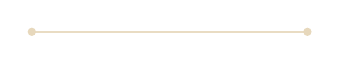
\begin{tikzpicture}
    \draw[GoldMain!40,line width=0.7pt] (0,0) -- (3.5,0);
    \fill[GoldMain!45] (0,0) circle (1.5pt);
    \fill[GoldMain!45] (3.5,0) circle (1.5pt);
  \end{tikzpicture}
  \vspace{0.8cm}
  {\large\color{GoldMain!80} \par}
  \vspace{0.5cm}
  {\small\color{GoldMed!80}
    依据扫描版原书逐页录入的 LaTeX 重排本\par}
\end{minipage}

% ============================================================
%  第七层：右下角 logo
% ============================================================
\begin{tikzpicture}[remember picture, overlay]
  \begin{scope}[shift={([xshift=-5.5cm, yshift=1.5cm]current page.south east)}]
    \draw[BlueMain, line width=0.8pt] (0,0) rectangle (0.9,0.72);
    \draw[BlueMain, line width=0.8pt] (0,0.72) -- (0.45,1.08) -- (0.9,0.72);
    \draw[GoldMain, line width=0.5pt] (0.45,0.72) -- (0.45,1.08);
    \draw[BlueMain, line width=0.4pt] (0.23,0) -- (0.23,0.72);
    \draw[BlueMain, line width=0.4pt] (0.67,0) -- (0.67,0.72);
    \fill[GoldMain] (0.45,1.08) circle (1.5pt);
    \node[anchor=west, BlueMain, font=\footnotesize] at (1.1,0.32)
      {定性理论 · 重排本};
  \end{scope}
\end{tikzpicture}

% ============================================================
%  第八层：底部封面图片
% ============================================================
\ifdefempty{\@coverimage}{}{
	\begin{tikzpicture}[remember picture,overlay]
		\node[anchor=south west,inner sep=0pt,outer sep=0pt]
			at ([xshift=3.3cm,yshift=3.05cm]current page.south west)
		{
			\includegraphics[
				width=\dimexpr\paperwidth-4.8cm\relax
			]{\@coverimage}
		};
	\end{tikzpicture}
}

% ============================================================
%  第九层：散落装饰点
% ============================================================
\begin{tikzpicture}[remember picture,overlay]
  \fill[GoldMain!18] ([xshift=-3.0cm,yshift=-9.5cm]current page.north west) circle (1.0pt);
  \fill[BlueLight!18] ([xshift=-3.8cm,yshift=-9.8cm]current page.north west) circle (0.7pt);
  \fill[GoldMain!16] ([xshift=-2.5cm,yshift=-10.2cm]current page.north west) circle (0.8pt);
  \fill[BlueMain!12] ([xshift=-4.0cm,yshift=3.5cm]current page.south west) circle (1.2pt);
  \fill[GoldMain!13] ([xshift=-5.5cm,yshift=4.0cm]current page.south west) circle (0.9pt);
  \fill[GoldMain!20] ([xshift=14.5cm,yshift=-6.0cm]current page.north west) circle (1.0pt);
  \fill[BlueLight!16] ([xshift=14.0cm,yshift=-5.5cm]current page.north west) circle (0.6pt);
  \fill[GoldMain!18] ([xshift=15.0cm,yshift=-5.8cm]current page.north west) circle (0.8pt);
\end{tikzpicture}

\end{titlepage}
}
\makeatother

\addbibresource{bibliography/references.bib}

% ============================================
%  封面配置
% ============================================
\seriestitle{数学经典 · LaTeX 重排}
\booktitle{微分方程定性理论}
\bookauthor{张芷芬、丁同仁、黄文灶、董镇喜}
\bookdate{\today}
\coverimage{}   % 放入 figure/封面.png 后填写路径即可

\begin{document}

% ── 生成封面 ──
\makecover

% ── 前置部分 ──
\frontmatter

\chapter*{重排说明}
\addcontentsline{toc}{chapter}{重排说明}

本文件是张芷芬、丁同仁、黄文灶、董镇喜著《微分方程定性理论》的
LaTeX 重排本，依据扫描版原书逐页录入，力求在版式、公式与符号上
与原书保持一致。

原书是平面自治系统定性理论的经典教材，系统阐述奇点分析、奇点指数、
极限环、无穷远奇点、周期系统的调和解、环面上的动力系统以及结构稳定性等
核心课题。全书以相平面上的向量场与积分曲线为几何出发点，强调不求解而通过
拓扑与解析方法判断轨线性态的思想。

本重排本按原书八章结构组织，正文分节与原书小节一一对应，章末的习题与
参考文献亦照原书录入。所有定理、定义、引理、示例等沿用统一的绛紫—香槟金
编号环境，以便于阅读与校订。

以下为正文。

\begin{flushright}
	LaTeX 录入重排\\
	\today
\end{flushright}

% ── 目录 ──
\tableofcontents
\newpage

% ============================================
%  正文部分
%  张芷芬《微分方程定性理论》八章结构（忠实转录）
% ============================================
\mainmatter
\setcounter{page}{1}

% 第一章  基本定理
% ============================================================
%  chapter01.tex — 第一章 基本定理
%  对应原书第一章。
%  本章建立全书的基础：解的存在唯一性、延拓、动力系统概念、
%  以及平面动力系统。
% ============================================================

\setchapterimage{}
\setchapterintro{}
\chapter{基本定理}
\renewcommand{\thesection}{\arabic{section}}
\newcommand{\sourceSection}[1]{%
  \refstepcounter{section}%
  \section*{\S\ \arabic{section}.\ #1}%
  \addcontentsline{toc}{section}{\arabic{section}. #1}%
}

本章介绍关于微分方程的解的一些基本定理，这是常微分方程一般理论的基础。

% ============================================================
%  §1  解的存在性、唯一性及对初值(或参数)的依赖性
% ============================================================
\sourceSection{解的存在性、唯一性及对初值(或参数)的依赖性}

\begin{theorem}{}{cauchy-exist}
	考虑 Cauchy 问题 $(E)$：
	\[
		\begin{cases}
			\dfrac{\dd \vect{x}}{\dd t} = \vect{f}(t,\vect{x}), \\[4pt]
			\vect{x}(t_0) = \vect{x}_0,
		\end{cases}
		\tag{1.1}
	\]
	其中 $\vect{x}$ 是 $\R^n$ 中的向量，$\vect{f}(t,\vect{x})$ 是实变量 $t$ 和 $n$ 维向量 $\vect{x}$ 的 $n$ 维向量值函数；又设 $\vect{f}(t,\vect{x})$ 在闭区域 $G$：
	\[
		|t - t_0| \leq a, \qquad \|\vect{x} - \vect{x}_0\| \leq b,
	\]
	上连续，并且对 $\vect{x}$ 适合 Lipschitz 条件：
	\[
		\|\vect{f}(t,\vect{x}_1) - \vect{f}(t,\vect{x}_2)\| 
		\leq L\|\vect{x}_1 - \vect{x}_2\|,
		\quad (t,\vect{x}_i) \in G,\ i = 1,2,
		\tag{1.2}
	\]
	其中 Lipschitz 常数 $L>0$。令
	\[
		M = \max_G \|\vect{f}(t,\vect{x})\|, \qquad 
		h = \min\!\left(a,\ \frac{b}{M}\right).
		\tag{1.3}
	\]
	那末 Cauchy 问题 $(E)$ 在区间 $|t-t_0|\leq h$ 上有一个解 $\vect{x}=\vect{\varphi}(t)$，并且它是唯一的。
\end{theorem}

\begin{proof}
	我们分以下五个步骤证明之。

	\textbf{（一）Cauchy 问题 $(E)$ 等价于积分方程}
	\[
		\vect{x} = \vect{x}_0 + \int_{t_0}^t \vect{f}(t,\vect{x})\,\dd t.
		\tag{1.4}
	\]

	事实上，令 $\vect{x} = \vect{\varphi}(t)$ 是 Cauchy 问题 $(E)$ 的解，于是由 (1.1) 对 $t$ 积分便有
	\[
		\vect{\varphi}(t) = \vect{C} + \int_{t_0}^t \vect{f}(t,\vect{\varphi}(t))\,\dd t,
	\]
	再由初值条件 (1.2) 确定 $\vect{C} = \vect{x}_0$，因此 $\vect{x} = \vect{\varphi}(t)$ 是（E）的解。

	反之，设 $\vect{x} = \vect{\varphi}(t)$ 是积分方程 (1.4) 的解，从 (1.4) 可知 $\vect{\varphi}(t)$ 是连续的，从而 $\vect{f}(t,\vect{\varphi}(t))$ 也是连续的，因此 $\vect{\varphi}(t)$ 是可微的；于是，对积分方程 (1.4) 的两侧对 $t$ 求导数，便得到
	\[
		\vect{\varphi}'(t) = \vect{f}(t,\vect{\varphi}(t)),
	\]
	并且由 (1.4) 可见 $\vect{x} = \vect{\varphi}(t)$ 满足初值条件
	\[
		\vect{\varphi}(t_0) = \vect{x}_0,
	\]
	即 $\vect{\varphi}(t)$ 是 Cauchy 问题 $(E)$ 的解。

	\textbf{（二）作 (1.4) 的 Picard 近似解序列 $\{\vect{\varphi}_n(t)\}$}

	令 $\vect{\varphi}_0(t) \equiv \vect{x}_0$，
	\[
		\vect{\varphi}_1(t) = \vect{x}_0 + \int_{t_0}^t \vect{f}(t,\vect{x}_0)\,\dd t,\quad
		|t - t_0| \leq h.
		\tag{1.5}
	\]
	则
	\[
		\|\vect{\varphi}_1(t) - \vect{\varphi}_0(t)\| 
		\leq \left|\int_{t_0}^t \|\vect{f}(t,\vect{x}_0)\|\,\dd t\right|
		\leq M \cdot |t - t_0| \leq b.
		\tag{1.6}
	\]

	当 $\vect{x}$ 是一维时，图形如下：


\begin{center}
	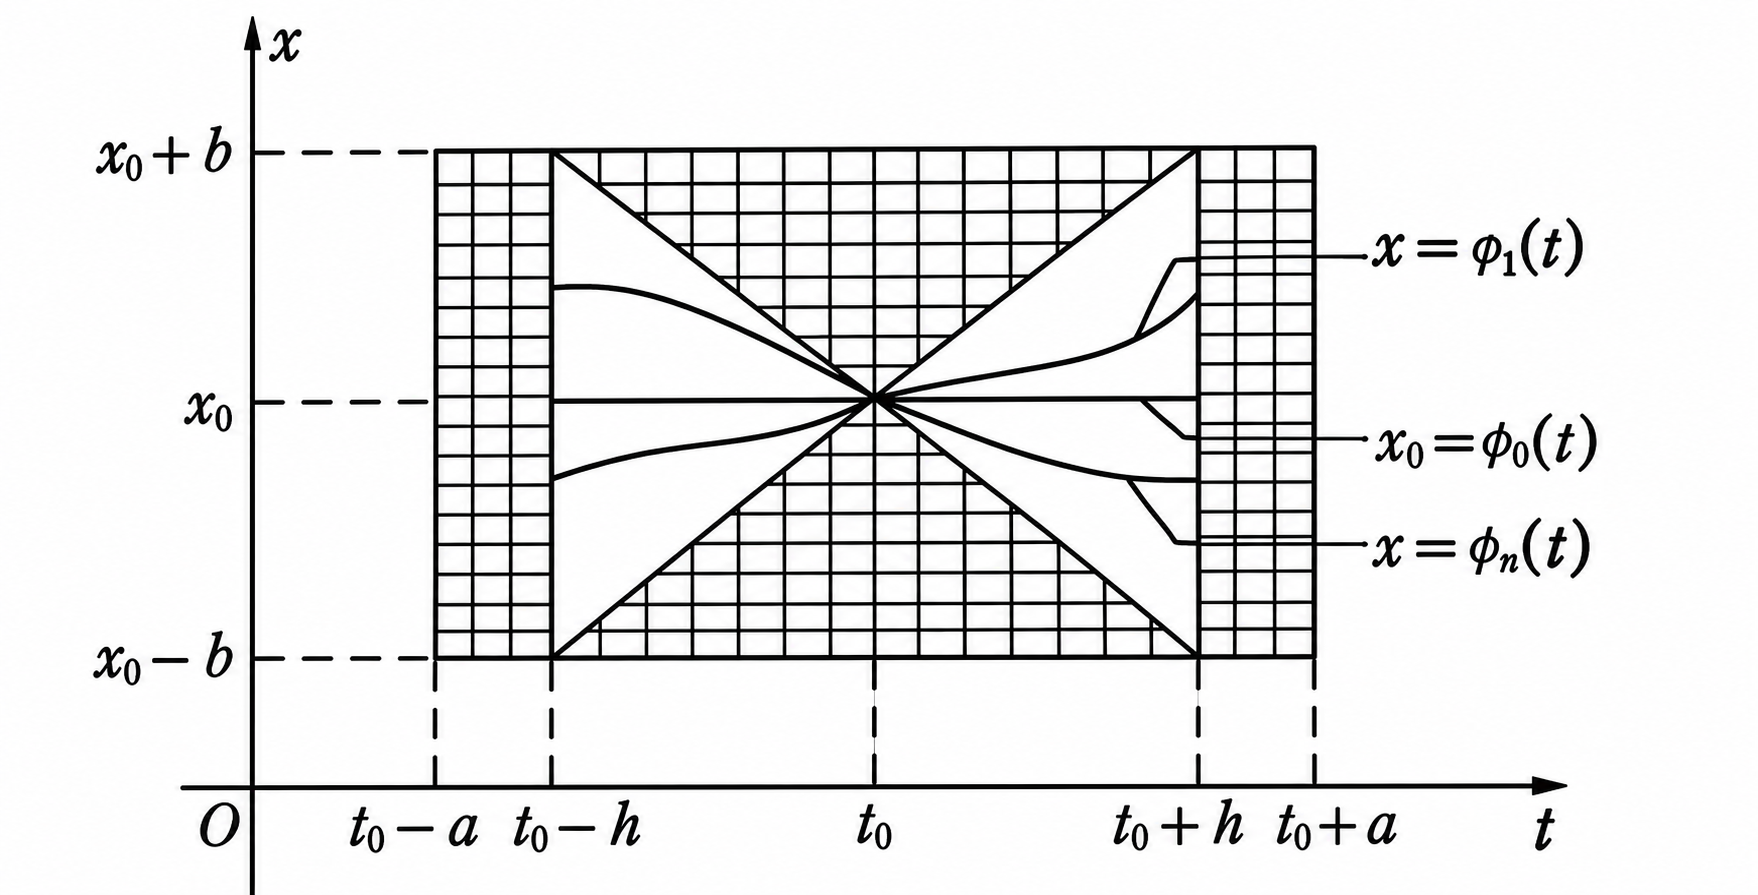
\includegraphics[width=0.7\linewidth]{figure/1}
	\captionof{figure}{}
\end{center}

	我们可以采用归纳的程序：设已得第 $n$ 次近似解为
	\[
		\vect{\varphi}_n(t) = \vect{x}_0 + \int_{t_0}^t \vect{f}(t,\vect{\varphi}_{n-1}(t))\,\dd t,
		\tag{1.7}
	\]
	而且当 $|t - t_0| \leq h$ 时，我们有
	\[
		\|\vect{\varphi}_n(t) - \vect{x}_0\| \leq b.
	\]
	令第 $n + 1$ 次近似解为
	\[
		\vect{\varphi}_{n+1}(t) = \vect{x}_0 + \int_{t_0}^t \vect{f}(t,\vect{\varphi}_n(t))\,\dd t,
		\tag{1.8}
	\]
	则当 $|t - t_0| \leq h$ 时，我们有
	\begin{align*}
		\|\vect{\varphi}_{n+1}(t) - \vect{x}_0\|
		&\leq \left\|\int_{t_0}^t \vect{f}(t,\vect{\varphi}_n(t))\,\dd t\right\| \\
		&\leq M \cdot |t - t_0| \leq Mh \leq b, \quad n = 1, 2, 3,\cdots.
	\end{align*}

	\textbf{（三）序列 $\{\vect{\varphi}_n(t)\}$ 的一致收敛性}

	由于 $\{\vect{\varphi}_n(t)\}$ 的收敛问题等价于级数
	\begin{align*}
		&\vect{\varphi}_0(t) + [\vect{\varphi}_1(t) - \vect{\varphi}_0(t)] 
		+ [\vect{\varphi}_2(t) - \vect{\varphi}_1(t)] \\
		&+ \cdots + [\vect{\varphi}_n(t) - \vect{\varphi}_{n-1}(t)] + \cdots
		\tag{1.9}
	\end{align*}
	的收敛问题，我们只要证明 (1.9) 的一致收敛性即可。

	首先证明 (1.9) 的一般项满足
	\[
		\|\vect{\varphi}_n(t) - \vect{\varphi}_{n-1}(t)\| 
		\leq \frac{M}{L}\,\frac{(L|t - t_0|)^n}{n!}, \quad n = 1, 2, 3,\cdots.
		\tag{1.10}
	\]
	由 (1.6) 可知 (1.10) 对 $n = 1$ 成立。假设不等式 (1.10) 对 $n = m$ 成立，则我们有下述不等式：
	\begin{align*}
		\|\vect{\varphi}_{m+1}(t) - \vect{\varphi}_m(t)\|
		&= \left\|\int_{t_0}^t \bigl(\vect{f}(t,\vect{\varphi}_m(t)) 
			- \vect{f}(t,\vect{\varphi}_{m-1}(t))\bigr)\,\dd t\right\| \\
		&\leq L \cdot \left|\int_{t_0}^t \|\vect{\varphi}_m(s) - \vect{\varphi}_{m-1}(s)\|\,\dd t\right| \\
		&\leq \frac{M}{L}\,\frac{(L|t - t_0|)^{m+1}}{(m+1)!}.
	\end{align*}
	由此可知不等式 (1.10) 对所有正整数 $n$ 都成立。所以当 $|t - t_0| \leq h$ 时，我们得到
	\[
		\|\vect{\varphi}_n(t) - \vect{\varphi}_{n-1}(t)\| 
		\leq \frac{M}{L}\,\frac{(Lh)^n}{n!}.
		\tag{1.11}
	\]
	由 Weierstrass 判别法推出级数 (1.9) 是一致收敛的，从而序列 $\{\vect{\varphi}_n(t)\}$ 一致收敛。令 $\lim_{n \to \infty} \vect{\varphi}_n(t) = \vect{\varphi}(t)$，则 $\vect{x} = \vect{\varphi}(t)$ 连续，且 $\|\vect{\varphi}(t) - \vect{x}_0\| \leq b\ (|t - t_0| \leq h)$。

	\textbf{（四）证明 $\vect{x} = \vect{\varphi}(t)$ 是积分方程 (1.4) 的解}

	令 $n \to +\infty$，由 (1.8) 得
	\[
		\vect{\varphi}(t) = \vect{x}_0 + \lim_{n \to \infty} \int_{t_0}^t 
			\vect{f}(t,\vect{\varphi}_n(t))\,\dd t.
		\tag{1.12}
	\]
	因此，归结于证明
	\[
		\lim_{n \to \infty} \int_{t_0}^t \vect{f}(t,\vect{\varphi}_n(t))\,\dd t 
		= \int_{t_0}^t \vect{f}(t,\vect{\varphi}(t))\,\dd t.
		\tag{1.13}
	\]
	任给 $\varepsilon > 0$，可找到 $N = N(\varepsilon) > 0$，使得当 $|t - t_0| \leq h$，便有不等式
	\[
		\|\vect{\varphi}_n(t) - \vect{\varphi}(t)\| \leq \frac{\varepsilon}{Lh}, 
		\quad \text{只要}\ n \geq N.
	\]
	因此，当 $|t - t_0| \leq h$ 时，我们有
	\begin{align*}
		&\left\|\int_{t_0}^t \vect{f}(t,\vect{\varphi}_n(t))\,\dd t 
			- \int_{t_0}^t \vect{f}(t,\vect{\varphi}(t))\,\dd t\right\| \\
		&\leq L \cdot \left|\int_{t_0}^t \|\vect{\varphi}_n(s) - \vect{\varphi}(s)\|\,\dd s\right| \\
		&\leq L \cdot \frac{\varepsilon}{L \cdot h} \cdot h = \varepsilon,
	\end{align*}
	即 (1.13) 成立。因此由 (1.12) 和 (1.3)，可见 $\vect{x} = \vect{\varphi}(t)$ 是积分方程 (1.4) 的一个解（$|t - t_0| \leq h$）。

	\textbf{（五）最后证明 (1.4) 的解的唯一性}

	事实上，设 $\vect{x} = \vect{\varphi}(t)$ 与 $\vect{x} = \vect{\psi}(t)$ 是 (1.4) 的两个解，即
	\[
		\vect{\varphi}(t) = \vect{x}_0 + \int_{t_0}^t \vect{f}(t,\vect{\varphi}(t))\,\dd s,
	\]
	与
	\[
		\vect{\psi}(t) = \vect{x}_0 + \int_{t_0}^t \vect{f}(t,\vect{\psi}(t))\,\dd t.
	\]
	两式相减，再利用 Lipschitz 条件，我们得到
	\[
		\|\vect{\varphi}(t) - \vect{\psi}(t)\| 
		\leq L \cdot \left|\int_{t_0}^t \|\vect{\varphi}(s) - \vect{\psi}(s)\|\,\dd t\right|.
		\tag{1.14}
	\]
	令
	\[
		g(t) = \int_{t_0}^t \|\vect{\varphi}(s) - \vect{\psi}(s)\|\,\dd t, \quad t \geq t_0.
	\]
	于是当 $t \geq t_0$ 时，$g(t) \geq 0$，而且 (1.14) 转化为
	\[
		g'(t) \leq L \cdot g(t),
		\tag{1.15}
	\]
	于是
	\[
		\bigl(e^{-L(t - t_0)} \cdot g(t)\bigr)' \leq 0,
	\]
	因而
	\[
		e^{-L(t - t_0)} \cdot g(t) \leq g(t_0) = 0.
	\]
	由此推出
	\[
		g(t) \equiv 0, \quad t \geq t_0,
	\]
	即
	\[
		\vect{\varphi}(t) \equiv \vect{\psi}(t), \quad t \geq t_0.
	\]
	同法可证：当 $t \leq t_0$ 时，$\vect{\varphi}(t) \equiv \vect{\psi}(t)$。

	总结以上各步骤，定理证毕。
\end{proof}

\fuzhu{1}{定理(1.1) 的证明是古典的，但可以抽象为泛函分析中的不动点定理。等式
\[
	\vect{\psi}(t) = \vect{x}_0 + \int_{t_0}^t \vect{f}(t,\vect{\varphi}(t))\,\dd t, 
	\quad |t - t_0| \leq h,
\]
定义了一个从连续函数 $\vect{\varphi}(t)$ 到连续函数 $\vect{\psi}(t)$ 的变换，可简写为
\[
	\vect{\psi} = \vect{T}(\vect{\varphi}).
\]
若 $\vect{T}(\vect{\varphi}) = \vect{\varphi}$，则称 $\vect{\varphi}$ 为变换 $\vect{T}$ 的不动点。显然 (1.4) 的解就是变换 $\vect{T}$ 的不动点。近代泛函分析中有各式各样的不动点定理，现介绍其中一个最简单的，称为\textbf{压缩映象原理}。

	设 $D$ 是 Banach 空间 $\mathscr{B}$ 的一个非空闭子集，$\vect{T}$ 是从 $D$ 到 $D$ 自身的映象，即对每一个 $\vect{\varphi} \in D$，有 $\vect{T}(\vect{\varphi}) \in D$。又存在常数 $k$，$0 \leq k < 1$，使对 $D$ 中任何两点 $\vect{\varphi}_1, \vect{\varphi}_2$，都有不等式
\[
	\|\vect{T}(\vect{\varphi}_1) - \vect{T}(\vect{\varphi}_2)\| \leq k\|\vect{\varphi}_1 - \vect{\varphi}_2\|.
\]
则在 $D$ 中存在唯一的一个点 $\vect{\varphi}^*$，使得 $\vect{T}(\vect{\varphi}^*) = \vect{\varphi}^*$。

	现在我们用上述压缩映象原理来证明定理(1.1)。取 $\mathscr{B}$ 为定义在区间 $|t - t_0| \leq a$ 上的一切连续函数所成的空间，取 $D$ 为定义在 $|t - t_0| \leq h^*$ 上 $\bigl(0 < h^* < \min(h, 1/L)\bigr)$ 而图象包含在 $G$ 中（见定理(1.1) 的条件）的一切连续函数所组成的集合。如果 $\vect{\varphi}(t) \in D$，定义
\[
	\vect{T}(\vect{\varphi}) = \vect{x}_0 + \int_{t_0}^t \vect{f}(\xi,\vect{\varphi}(\xi))\,\dd\xi,
\]
则
\[
	\|\vect{T}(\vect{\varphi}) - \vect{x}_0\| 
	\leq \left\|\int_{t_0}^t \vect{f}(\xi,\vect{\varphi}(\xi))\,\dd\xi\right\|
	\leq M|t - t_0| \leq Mh \leq b,
\]
即 $\vect{T}(\vect{\varphi}) \in D$。其次设 $\vect{\varphi}_1, \vect{\varphi}_2 \in D$，于是
\begin{align*}
	\|\vect{T}(\vect{\varphi}_1) - \vect{T}(\vect{\varphi}_2)\| 
	&\leq \left|\int_{t_0}^t \|\vect{f}(t,\vect{\varphi}_1) - \vect{f}(t,\vect{\varphi}_2)\|\,\dd t\right| \\
	&\leq L \cdot h^* \|\vect{\varphi}_1 - \vect{\varphi}_2\| \\
	&= K \|\vect{\varphi}_1 - \vect{\varphi}_2\|, \quad (K = Lh^* < 1).
\end{align*}
故由压缩映象原理，有唯一的不动点 $\vect{\varphi}^*$，使 $\vect{T}(\vect{\varphi}^*) = \vect{\varphi}^*$，即
\[
	\vect{\varphi}^*(t) = \vect{x}_0 + \int_{t_0}^t \vect{f}(t,\vect{\varphi}^*(t))\,\dd t, 
	\quad (|t - t_0| \leq h^*).
	\]
}

\fuzhu{2}{设方程 (1.1) 是线性的，即
\[
	\frac{\dd \vect{x}}{\dd t} = \vect{A}(t)\vect{x} + \vect{f}(t),
	\tag{1.16}
\]
其中 $\vect{A}(t), \vect{f}(t)$ 在区间 $[\alpha, \beta]$ 上是连续的。

这时由初值 $(t_0, \vect{x}_0)\ (t_0 \in [\alpha, \beta])$ 所确定的解在整个区间 $[\alpha, \beta]$ 上都有定义。这是因为所构造的逐次近似解序列 $\{\vect{\varphi}_n(t)\}$ 在整个区间 $[\alpha, \beta]$ 都有定义，并且是一致收敛的。}

\fuzhu{3}{如果 $\vect{f}(t, \vect{x})$ 对 $t, \vect{x}$ 连续，但不一定满足 Lipschitz 条件，则 Cauchy 问题 (1.1) + (1.2) 的解仍是存在的，参见下面的定理（证明从略）。}
\namedthm{Cauchy-Peano}{若 $\vect{f}(t, \vect{x})$ 在区域 $G: |t - t_0| \leq a, \|\vect{x} - \vect{x}_0\| \leq b$ 上连续，则 (1.4) 在区间 $|t - t_0| \leq h$ 上有解 $\vect{x} = \vect{\varphi}(t)$ 且满足初值条件 $\vect{\varphi}(t_0) = \vect{x}_0$，此处
	若 $\vect{f}(t, \vect{x})$ 在区域 $G: |t - t_0| \leq a, \|\vect{x} - \vect{x}_0\| \leq b$ 上连续，则 (1.4) 在区间 $|t - t_0| \leq h$ 上有解 $\vect{x} = \vect{\varphi}(t)$ 且满足初值条件 $\vect{\varphi}(t_0) = \vect{x}_0$，此处
\[
h = \min\!\left(a,\ \frac{b}{M}\right), \qquad 
M = \max_G \|\vect{f}(t,\vect{x})\|.
\]
}


下面讨论解与参数（或初值）的关系。

考虑方程
\[
	\begin{cases}
		\dfrac{\dd \vect{x}}{\dd t} = \vect{f}(t, \vect{x}), \\[4pt]
		\vect{x}(t_0) = \vect{x}_0,
	\end{cases}
\]
的解 $\vect{x} = \vect{\varphi}(t, t_0, \vect{x}_0)$。这个解是 $t, t_0, \vect{x}_0$ 的函数。例如方程
\[
	\begin{cases}
		\dfrac{\dd \vect{x}}{\dd t} = \vect{x}, \\[4pt]
		\vect{x}(t_0) = \vect{x}_0,
	\end{cases}
\]
的解为 $\vect{x} = \vect{x}_0 e^{t - t_0}$，它是 $t, t_0, \vect{x}_0$ 的函数。

这里发生了一个在理论上和应用上都很重要的问题：当初值或参数变动时，对应的解是如何变动的？我们知道，在应用上，微分方程是描述某种物理过程的。而将一个物理问题化成微分方程问题时，不论是初值还是参数，它们的数值都是由实验测定的，因此不可避免地会出现一些微小的误差。如果初值或参数的微小振动会引起方程的解发生剧烈的变化，那么所求解的可靠性就会很小。因此我们要研究 Cauchy 问题的解与初值或参数的关系是自然而必要的。

\begin{theorem}{}{param-cont}
	考虑 Cauchy 问题 $(E_{\vect{\mu}})$：
	\[
		\frac{\dd \vect{x}}{\dd t} = \vect{f}(t, \vect{x}, \vect{\mu}), \qquad 
		\vect{x}(t_0) = \vect{x}_0,
		\tag{1.17}
	\]
	此处 $\vect{x}$ 是 $\R^n$ 中的 $n$ 维向量，$\vect{\mu}$ 是 $\R^m$ 中的 $m$ 维向量。函数 $\vect{f}(t, \vect{x}, \vect{\mu})$ 在区域 $G$：
	\[
		|t - t_0| \leq a,\quad \|\vect{x} - \vect{x}_0\| \leq b,\quad \|\vect{\mu} - \vect{\mu}_0\| \leq c,
	\]
	上连续且对 $\vect{x}$ 适合 Lipschitz 条件：
	\[
		\|\vect{f}(t, \vect{x}_1, \vect{\mu}) - \vect{f}(t, \vect{x}_2, \vect{\mu})\| 
		\leq L\|\vect{x}_1 - \vect{x}_2\|, \quad \forall(t, \vect{x}_i, \vect{\mu}) \in G,\ i = 1,2,
	\]
	其中 Lipschitz 常数 $L > 0$。令
	\[
		M = \max_G \|\vect{f}(t, \vect{x}, \vect{\mu})\|, \qquad 
		h = \min\!\left(a,\ \frac{b}{M}\right),
	\]
	则对于任意 $\vect{\mu}\,(\|\vect{\mu} - \vect{\mu}_0\| \leq c)$，$(E_{\vect{\mu}})$ 的解 $\vect{x} = \vect{x}(t; \vect{\mu})$ 在区间 $|t - t_0| \leq h$ 上存在且唯一，并且 $\vect{x} = \vect{x}(t; \vect{\mu})$ 是 $(t, \vect{\mu})$ 的连续函数。
\end{theorem}

\begin{proof}
	对任意 $\vect{\mu}\,(\|\vect{\mu} - \vect{\mu}_0\| \leq c)$，根据定理~\ref{thm:cauchy-exist}，$(E_{\vect{\mu}})$ 的解 $\vect{x} = \vect{x}(t; \vect{\mu})$ 在 $|t - t_0| \leq h$ 上存在唯一。

	又因为 Cauchy 问题 $(E_{\vect{\mu}})$ 的 $n$ 次近似解 $\vect{x} = \vect{\varphi}_n(t; \vect{\mu})$ 是 $(t, \vect{\mu})$ 的连续函数而且当 $n \to +\infty$ 时，$\vect{\varphi}_n(t; \vect{\mu})$ 在区域 $(|t - t_0| \leq h, \|\vect{\mu} - \vect{\mu}_0\| \leq c)$ 上一致收敛，因而 $\vect{\varphi}(t; \vect{\mu})$ 是 $(t, \vect{\mu})$ 的连续函数。
\end{proof}

\namedlem{Grownwall}{设函数 $g(t), \varphi(t)$ 是区间 $[t_0, t_1]$ 上的连续函数，而且 $g(t) \geq 0, \varphi(t) \geq 0$；又常数 $\lambda > 0, r > 0$。若 $\varphi(t)$ 满足不等式
	设函数 $g(t), \varphi(t)$ 是区间 $[t_0, t_1]$ 上的连续函数，而且 $g(t) \geq 0, \varphi(t) \geq 0$；又常数 $\lambda > 0, r > 0$。若 $\varphi(t)$ 满足不等式
\[
\varphi(t) \leq \lambda + \int_{t_0}^t (g(t)\varphi(t) + r)\,\dd s, \quad t_0 \leq t \leq t_1,
\tag{1.18}
\]
则有
\[
\varphi(t) \leq (\lambda + rT)\,e^{\int_{t_0}^t g(s)\,\dd s}, \quad t_0 \leq t \leq t_1,
\tag{1.19}
\]
其中 $T = t_1 - t_0$。
}

\begin{proof}
	令 $u(t) = \varphi(t)\,e^{-\int_{t_0}^t g(s)\,\dd s}$，$t_0 \leq t \leq t_1$，显然 $u(t)$ 是连续的。设 $\xi = \sup\{u(t)\}_{t_0 \leq t \leq t_1}$，则存在 $t^* \in [t_0, t_1]$，使得 $u(t^*) = \xi$。由 (1.18) 得
	\begin{align*}
		\xi\,e^{\int_{t_0}^{t^*} g(s)\,\dd s} 
		&\leq \lambda + \int_{t_0}^{t^*} (g(s)\varphi(s) + r)\,\dd s \\
		&\leq \lambda + \int_{t_0}^{t^*} \bigl(\xi\,g(s)\,e^{\int_{t_0}^s g(s)\,\dd s} + r\bigr)\,\dd s \\
		&\leq \lambda + rT + \xi\bigl(e^{\int_{t_0}^{t^*} g(s)\,\dd s} - 1\bigr),
	\end{align*}
	即
	\[
		\xi \leq \lambda + rT.
	\]
	由于
	\[
		\varphi(t) \leq \xi\,e^{\int_{t_0}^t g(s)\,\dd s},
	\]
	故
	\[
		\varphi(t) \leq (\lambda + rT)\,e^{\int_{t_0}^t g(s)\,\dd s}.
	\]
\end{proof}

\begin{theorem}{}{param-diff}
	设 Cauchy 问题 $(E_{\vect{\mu}}^*)$：
	\[
		\frac{\dd \vect{x}}{\dd t} = \vect{f}(t, \vect{x}, \vect{\mu}), \qquad 
		\vect{x}(t_0) = \vect{x}_0,
	\]
	其中 $\vect{x}$ 是 $\R^n$ 中的 $n$ 维向量，$\vect{\mu}$ 是 $\R^m$ 中的 $m$ 维向量。又设 $\vect{f}(t, \vect{x}, \vect{\mu}) \in C^0(G, \R^n)$，其中
	\[
		G:\ |t - t_0| \leq a,\ \|\vect{x} - \vect{x}_0\| \leq b,\ \|\vect{\mu} - \vect{\mu}_0\| \leq c,
	\]
	且 $\dfrac{\partial \vect{f}}{\partial x_j}\ (j = 1, 2, \cdots, n)$，$\dfrac{\partial \vect{f}}{\partial \mu_k}\ (k = 1, 2, \cdots, m)$ 连续，则定理~\ref{thm:param-cont} 的结论成立，而且 $\vect{x} = \vect{x}(t, \vect{\mu})$ 对 $\mu_k\ (k = 1, 2, \cdots, m)$ 有连续的偏导数。
\end{theorem}

\begin{proof}
	因为 $\dfrac{\partial \vect{f}}{\partial x_j} \in C^0(G, \R^n)\ (j = 1, 2, \cdots, n)$，所以 $\vect{f}$ 对 $\vect{x}$ 适合 Lipschitz 条件。因此，定理~\ref{thm:param-cont} 蕴含定理~\ref{thm:param-diff}，即 $(E_{\vect{\mu}}^*)$ 的解 $\vect{x} = \vect{\varphi}(t, \vect{\mu})$ 存在唯一且在区域 $B(|t - t_0| \leq h, \|\vect{\mu} - \vect{\mu}_0\| \leq c)$ 上连续。下面证明 $\vect{x} = \vect{\varphi}(t, \vect{\mu})$ 对 $\vect{\mu}$ 是可微的。我们的证明分以下三个步骤进行。

	为了形式地推导 $\dfrac{\partial \vect{x}}{\partial \vect{\mu}}$，首先我们考虑线性方程
	\[
		\begin{cases}
			\dfrac{\dd \vect{z}}{\dd t} 
			= \vect{f}_{\vect{x}}(t, \vect{\varphi}(t, \vect{\mu}), \vect{\mu})\,\vect{z} 
			+ \vect{f}_{\vect{\mu}}(t, \vect{\varphi}(t, \vect{\mu}), \vect{\mu}), \\[4pt]
			\vect{z}(t_0) = \vect{0},
		\end{cases}
	\]
	或与上面等价的积分方程
	\[
		\vect{z}(t, \vect{\mu}) 
		= \int_{t_0}^t \bigl[\vect{f}_{\vect{x}}(t, \vect{\varphi}(t, \vect{\mu}), \vect{\mu})\,\vect{z}(t, \vect{\mu})
		+ \vect{f}_{\vect{\mu}}(t, \vect{\varphi}(t, \vect{\mu}), \vect{\mu})\bigr]\,\dd t,
		\tag{1.20}
	\]
	其中
	\[
		\vect{f}_{\vect{x}}(t, \vect{\varphi}(t, \vect{\mu}), \vect{\mu}) 
		= \left(\frac{\partial f_i(t, \vect{\varphi}(t, \vect{\mu}), \vect{\mu})}{\partial x_j}\right)_{n \times n}
	\]
	是 $n \times n$ 矩阵，
	\[
		\vect{f}_{\vect{\mu}}(t, \vect{\varphi}(t, \vect{\mu}), \vect{\mu}) 
		= \left(\frac{\partial f_i(t, \vect{\varphi}(t, \vect{\mu}), \vect{\mu})}{\partial \mu_k}\right)_{n \times m}
	\]
	是 $n \times m$ 矩阵。

	Cauchy 问题 $(E_0^{\vect{\mu}})$ 等价于积分方程
	\[
		\vect{x} = \vect{x}_0 + \int_{t_0}^t \vect{f}(t, \vect{x}, \vect{\mu})\,\dd t,
		\tag{1.21}
	\]
	从此式形式地计算 $\dfrac{\partial \vect{x}}{\partial \vect{\mu}}$ 得
	\[
		\frac{\partial \vect{x}}{\partial \vect{\mu}} 
		= \int_{t_0}^t \left(\frac{\partial \vect{f}(t, \vect{\varphi}(t, \vect{\mu}), \vect{\mu})}{\partial \vect{x}}\,\frac{\partial \vect{x}}{\partial \vect{\mu}}
		+ \frac{\partial \vect{f}(t, \vect{\varphi}(t, \vect{\mu}), \vect{\mu})}{\partial \vect{\mu}}\right)\dd t.
		\tag{1.22}
	\]
	这就是说，如果 $\dfrac{\partial \vect{x}}{\partial \vect{\mu}}$ 存在，则它应满足方程 (1.20)。

	其次，当参量 $\vect{\mu}$ 有改变量 $\Delta\vect{\mu}$ 时，相应的 $\vect{x}$ 有改变量 $\Delta\vect{x}$，令计算 $\Delta\vect{x}$.
	\begin{align*}
		\Delta\vect{x} 
		&= \vect{x}(t, \vect{\mu} + \Delta\vect{\mu}) - \vect{x}(t, \vect{\mu}) = \vect{\varphi} + \Delta\vect{\varphi} \\
		&= \int_{t_0}^t [\vect{f}(t, \vect{\varphi} + \Delta\vect{\varphi}, \vect{\mu} + \Delta\vect{\mu}) - \vect{f}(t, \vect{\varphi}, \vect{\mu})]\,\dd s \\
		&= \int_{t_0}^t \left(\frac{\partial \vect{f}(t, \vect{\varphi}, \vect{\mu})}{\partial \vect{x}} + \vect{\varepsilon}_1\right)\Delta\vect{x}\,\dd t \\
		&\quad + \int_{t_0}^t \left(\frac{\partial \vect{f}(t, \vect{\varphi}, \vect{\mu})}{\partial \vect{\mu}} + \vect{\varepsilon}_2\right)\Delta\vect{\mu}\,\dd t.
		\tag{1.23}
{\tiny }	\end{align*}
	其中 $\vect{\varepsilon}_1$ 是 $n \times n$ 矩阵，$\vect{\varepsilon}_2$ 是 $n \times m$ 矩阵，而且当 $\|\Delta\vect{\mu}\|$ 趋于零时，$\|\vect{\varepsilon}_1\|, \|\vect{\varepsilon}_2\|$ 一致地趋于零，即
	\[
		\lim_{\|\Delta\vect{\mu}\| \to 0} \|\vect{\varepsilon}_1\| = 0, \qquad 
		\lim_{\|\Delta\vect{\mu}\| \to 0} \|\vect{\varepsilon}_2\| = 0.
		\tag{1.24}
	\]
	把 $\vect{\varepsilon}_1, \vect{\varepsilon}_2$ 代入 (1.23) 便有下式：
	\begin{align*}
		\Delta\vect{x} 
		&= \int_{t_0}^t \left(\frac{\partial \vect{f}(t, \vect{\varphi}(t, \vect{\mu}), \vect{\mu})}{\partial \vect{x}} + \vect{\varepsilon}_1\right)\Delta\vect{x}\,\dd t \\
		&\quad + \int_{t_0}^t \left(\frac{\partial \vect{f}(t, \vect{\varphi}(t, \vect{\mu}), \vect{\mu})}{\partial \vect{\mu}} + \vect{\varepsilon}_2\right)\Delta\vect{\mu}\,\dd t.
		\tag{1.25}
	\end{align*}

	最后来证明
	\[
		\lim_{\|\Delta\vect{\mu}\| \to 0} \frac{\|\Delta\vect{x} - \vect{z}(t, \vect{\mu})\Delta\vect{\mu}\|}{\|\Delta\vect{\mu}\|} = 0.
	\]
	由 (1.20) 和 (1.25) 有
	\begin{align*}
		\Delta\vect{x} - \vect{z}(t, \vect{\mu})\Delta\vect{\mu} 
		= \int_{t_0}^t &\Bigl[\left(\frac{\partial \vect{f}}{\partial \vect{x}} + \vect{\varepsilon}_1\right)(\Delta\vect{x} - \vect{z}\Delta\vect{\mu}) \\
		&+ (\vect{\varepsilon}_1 \vect{z} + \vect{\varepsilon}_2)\Delta\vect{\mu}\Bigr]\dd s.
	\end{align*}
	令 $\Delta\vect{u} = \Delta\vect{x} - \vect{z}(t, \vect{\mu})\Delta\vect{\mu}$，于是上式化为
	\[
		\Delta\vect{u} = \int_{t_0}^t \left[\left(\frac{\partial \vect{f}}{\partial \vect{x}} + \vect{\varepsilon}_1\right)\Delta\vect{u} + (\vect{\varepsilon}_1 \vect{z} + \vect{\varepsilon}_2)\Delta\vect{\mu}\right]\dd t,
	\]
	因而
	\[
		\|\Delta\vect{u}\| \leq \left|\int_{t_0}^t \left[\left\|\frac{\partial \vect{f}}{\partial \vect{x}} + \vect{\varepsilon}_1\right\| \cdot \|\Delta\vect{u}\| + \|\vect{\varepsilon}_1 \vect{z} + \vect{\varepsilon}_2\| \cdot \|\Delta\vect{\mu}\|\right]\dd t\right|.
	\]
	令 $N = \max_G \left\|\dfrac{\partial \vect{f}}{\partial \vect{x}}\right\|$，又取正数 $\delta_1, \delta_2$，使得 $\|\vect{\varepsilon}_1\| \leq \delta_1,\ \|\vect{\varepsilon}_1 \vect{z} + \vect{\varepsilon}_2\| \leq \delta_2$，而且当 $\|\Delta\vect{\mu}\| \to 0$，$\delta_1 \to 0, \delta_2 \to 0$，因而
	\[
		\|\Delta\vect{u}\| \leq \left|\int_{t_0}^t [(N + \delta_1)\|\Delta\vect{u}\| + \delta_2\|\Delta\vect{\mu}\|]\dd t\right|.
	\]
	再由基本引理~\ref{lem:gronwall} 便得
	\[
		\|\Delta\vect{u}\| \leq \delta_2 \|\Delta\vect{\mu}\| \cdot h \cdot e^{\int_{t_0}^t (N + \delta_1)\dd s} 
		\leq \delta_2 \|\Delta\vect{\mu}\| h e^{(N + \delta_1)h}.
	\]
	由此推出，当 $\|\Delta\vect{\mu}\| \to 0$ 时我们有
	\[
		\frac{\|\Delta\vect{u}\|}{\|\Delta\vect{\mu}\|} 
		= \frac{\|\Delta\vect{x} - \vect{z}(t, \vect{\mu})\Delta\vect{\mu}\|}{\|\Delta\vect{\mu}\|} 
		\leq \delta_2 \cdot h \cdot e^{(N + \delta_1)h} \to 0,
	\]
	根据多元函数微分学的定义：我们有
	\[
		\dd\vect{x} = \vect{z}(t, \vect{\mu})\dd\vect{\mu},
	\]
	从而
	\[
		\frac{\partial \vect{x}}{\partial \vect{\mu}} = \vect{z}(t, \vect{\mu}).
	\]
	这样我们证明了 $\dfrac{\partial \vect{x}}{\partial \vect{\mu}}$ 是存在的，再对 (1.20) 利用定理~\ref{thm:param-cont}，可见 $\dfrac{\partial \vect{x}}{\partial \vect{\mu}}$ 对 $(t, \vect{\mu})$ 是连续的。定理证毕。
\end{proof}

\begin{theorem}{}{init-cont}
	考虑 Cauchy 问题 $(E_{\vect{\eta}})$：
	\[
		\begin{cases}
			\dfrac{\dd \vect{x}}{\dd t} = \vect{f}(t, \vect{x}), \\[4pt]
			\vect{x}(t_0) = \vect{\eta}, \qquad (\|\vect{\eta} - \vect{\eta}_0\| \leq b/2),
		\end{cases}
	\]
	其中 $\vect{f}(t, \vect{x})$ 在区域 $D\,(|t - t_0| \leq a, \|\vect{x} - \vect{x}_0\| \leq b)$ 上连续，且对 $\vect{x}$ 适合 Lipschitz 条件
	\[
		\|\vect{f}(t, \vect{x}_1) - \vect{f}(t, \vect{x}_2)\| \leq L \cdot \|\vect{x}_1 - \vect{x}_2\|,
		\quad \forall(t, \vect{x}_i) \in D,\ i = 1,2,
	\]
	其中 Lipschitz 常数 $L > 0$。令
	\[
		M = \max_D \|\vect{f}(t, \vect{x})\|, \qquad 
		h = \min\!\left(a,\ \frac{b}{M}\right),
	\]
	则对所有 $\vect{\eta}\,(\|\vect{\eta} - \vect{\eta}_0\| \leq b/2)$，$(E_{\vect{\eta}})$ 的解 $\vect{x} = \vect{x}(t, \vect{\eta})$ 在区间
	\[
		|t - t_0| \leq \tfrac{1}{2}h
	\]
	上存在，且 $\vect{x} = \vect{x}(t, \vect{\eta})$ 是 $(t, \vect{\eta})$ 的连续函数。
\end{theorem}

\begin{proof}
	令 $\vect{x} = \vect{z} + \vect{\eta}$（$\vect{z}$ 是新的未知 $n$ 维向量函数），则 $(E_{\vect{\eta}})$ 化成 $(\hat{E}_{\vect{\eta}})$：
	\[
		\frac{\dd \vect{z}}{\dd t} = \vect{F}(t, \vect{z}, \vect{\eta}), \qquad \vect{z}(t_0) = 0,
	\]
	其中 $\vect{F}(t, \vect{z}, \vect{\eta}) = \vect{f}(t, \vect{z} + \vect{\eta})$，在区域 $G$：
	\[
		|t - t_0| \leq a,\quad \|\vect{z}\| \leq \frac{b}{2},\quad \|\vect{\eta} - \vect{\eta}_0\| \leq \frac{b}{2},
	\]
	上连续，且
	\begin{align*}
		\|\vect{F}(t, \vect{z}_1, \vect{\eta}) - \vect{F}(t, \vect{z}_2, \vect{\eta})\| 
		&= \|\vect{f}(t, \vect{z}_1 + \vect{\eta}) - \vect{f}(t, \vect{z}_2 + \vect{\eta})\| \\
		&\leq L\|\vect{z}_1 + \vect{\eta} - (\vect{z}_2 + \vect{\eta})\| \\
		&= L\|\vect{z}_1 - \vect{z}_2\|.
	\end{align*}
	注意 $\vect{\eta}$ 对于 $(\hat{E}_{\vect{\eta}})$ 而言作为参数向量出现。因此，由定理~\ref{thm:param-cont} 推出，$(\hat{E}_{\vect{\eta}})$ 的解 $\vect{z} = \vect{\varphi}(t, \vect{\eta})$ 在区间 $|t - t_0| \leq \tfrac{1}{2}h$ 上存在（这里注意 $G$ 中的 $b/2$）；且 $\vect{z} = \vect{\varphi}(t, \vect{\eta})$ 是 $(t, \vect{\eta})$ 的连续函数。由于 $(E_{\vect{\eta}})$ 的解为
	\[
		\vect{x} = \vect{\varphi}(t, \vect{\eta}) = \vect{\psi}(t, \vect{\eta}) + \vect{\eta},
	\]
	所以定理~\ref{thm:init-cont} 证毕。
\end{proof}

\medskip
类似地可以考虑 Cauchy 问题 $(E_\xi)$：
\[
	\begin{cases}
		\dfrac{\dd \vect{x}}{\dd t} = \vect{f}(t, \vect{x}), \\[4pt]
		\vect{x}(\xi) = \vect{x}_0,
	\end{cases}
\]
对 $\xi$ 的依赖关系。

令 $t = \tau + \xi$，此处 $\tau$ 是新的自变量。于是把 Cauchy 问题 $(E_\xi)$ 化为：
\[
	\begin{cases}
		\dfrac{\dd \vect{x}}{\dd \tau} = \vect{f}(\tau + \xi, \vect{x}) = \vect{F}(\tau, \vect{x}, \xi), \\[4pt]
		\vect{x}(0) = \vect{x}_0,
	\end{cases}
\]
此处 $\xi$ 是参数。

\begin{theorem}{}{init-diff}
	若在定理 (1.4) 中的 $\vect{f}(t, \vect{x})$ 及其偏导数 $\dfrac{\partial \vect{f}}{\partial \vect{x}}$ 在 $D$ 上连续，则 $(E_{\vect{\eta}})$ 的解 $\vect{x} = \vect{\varphi}(t, \vect{\eta})$ 对 $\vect{\eta}$ 有连续的偏导数。
\end{theorem}

\begin{proof}
	只要注意，此时 $(\hat{E}_{\vect{\eta}})$ 满足定理~\ref{thm:param-diff} 的条件。
\end{proof}

\begin{theorem}{}{smooth}
	设定理 (1.3) 中方程右侧的函数 $\vect{f}(t, \vect{x}, \vect{\mu})$ 对 $t$ 而言是 $r - 1$ 次连续可微的，对 $\vect{x}$ 和 $\vect{\mu}$ 而言是 $r$ 次连续可微的（包括混合偏导数），则 Cauchy 问题 $(E_{\vect{\mu}}^*)$ 的解 $\vect{x} = \vect{\varphi}(t, t_0, \vect{x}_0, \vect{\mu})$ 对 $t, t_0, \vect{x}_0, \vect{\mu}$ 而言是 $r$ 次连续可微的。
\end{theorem}

\begin{proof}
	其证明办法是作原方程的变分方程，再对变分方程作变分方程，接连不断重复这一过程，并反复应用定理~\ref{thm:param-diff} 的讨论。
\end{proof}

\begin{theorem}{}{analytic}
	设 $\vect{f}(t, \vect{x}, \vect{\mu})$ 在区域 $G$ 内是 $t, \vect{x}, \vect{\mu}$ 的解析函数，则 Cauchy 问题 $(E_{\vect{\mu}}^*)$ 的解 $\vect{x} = \vect{\varphi}(t, t_0, \vect{x}_0, \vect{\mu})$ 是 $t, \vect{x}_0, t_0, \vect{\mu}$ 的解析函数。若 $\vect{f}(t, \vect{x}, \vect{\mu})$ 对 $t$ 只是连续的，则 $(E_{\vect{\mu}}^*)$ 的解只是对 $\vect{x}_0, \vect{\mu}$ 解析。
\end{theorem}

\begin{proof}
	请参考文献[4]第 32--37 页。
\end{proof}

% ============================================================
%  §2  解的延拓
% ============================================================
\sourceSection{解的延拓}

由定理~\ref{thm:cauchy-exist} 可知，在相当广泛的条件下，Cauchy 问题
\begin{equation*}
\left\{
\begin{aligned}
&\frac{\dd\vect{x}}{\dd t} = \vect{f}(t, \vect{x}) && \text{(2.1)}\\
&\vect{x}(t_0) = \vect{x}_0 && \text{(2.2)}
\end{aligned}
\right.
\end{equation*}
的解是存在的，但是值得注意的是，这是一个局部性的定理，因为定理所肯定的只是解在某个区间 $|t - t_0| \leq h$ 上存在。我们自然要问：能否将一个在小区间上有定义的解``延拓到比较大的区间上去呢''？

设 (2.1)+(2.2) 的解 $\vect{x} = \vect{\varphi}(t)$ 在 $[t_0 - h_0, t_0 + h_0]$ 上存在。记 $t_1 = t_0 + h_0$。考虑 Cauchy 问题
\[
\left\{
\begin{aligned}
\frac{\dd\vect{x}}{\dd t} &= \vect{f}(t, \vect{x}),\\
\vect{x}(t_1) &= \vect{x}_1,
\end{aligned}
\right.
\]
根据定理~\ref{thm:cauchy-exist}，上述 Cauchy 问题的解 $\vect{x} = \vect{\varphi}_1(t)$ 存在于区间 $[t_1 - h_1, t_1 + h_1]$。那么根据唯一性可知道，在两区间的重叠部分应有 $\vect{\varphi}_1(t) = \vect{\varphi}(t)$。然后定义
\[
\vect{\varphi}^*(t) = 
\begin{cases}
\vect{\varphi}(t), & \text{当 } t \in [t_0 - h_0, t_0 + h_0],\\
\vect{\varphi}_1(t), & \text{当 } t \in [t_1, t_1 + h_1].
\end{cases}
\]
于是 $\vect{\varphi}^*(t)$ 是 Cauchy 问题 (2.1)+(2.2) 在区间 $[t_0 - h_0, t_1 + h_1]$ 上的唯一解。同理可向左延拓一小段区间。如此继续下去，我们得到一个解 $\vect{x} = \overline{\vect{\varphi}}(t)$，它不能向左右两方再继续延拓了，得到了最大的存在区间 $(\alpha, \beta)$，要注意，它不能包含这个区间的左、右端点，因为否则就还可以延拓，所以总是一个最大的开区间。

$\vect{f}(t, \vect{x})$ 叫做在开区域 $G \subseteq \R \times \R^n$ 上对 $\vect{x}$ 满足\textbf{局部 Lipschitz 条件}，若对任给点 $A(t_0, \vect{x}_0) \in G$，存在实数 $a > 0,\ b > 0$，使得
\[
\{|t - t_0| \leq a,\ \|\vect{x} - \vect{x}_0\| \leq b\} \subset G,
\]
有 $\|\vect{f}(t, \vect{x}_1) - \vect{f}(t, \vect{x}_2)\| \leq L_A \|\vect{x}_1 - \vect{x}_2\|$，当 $|t - t_0| \leq a,\ \|\vect{x}_i - \vect{x}_0\| \leq b,\ i = 1, 2$，其中 $L_A$ 是与 $A$ 有关的常数。

\begin{theorem}{}{endpt-lim}
设 $\vect{f}(t, \vect{x})$ 在区域 $G$ 内有界，且对 $\vect{x}$ 满足局部 Lipschitz 条件。若 (2.1)+(2.2) 的解 $\vect{x} = \vect{\varphi}(t)$ 按照上述方法得到最大的存在区间为 $\alpha < t < \beta$，则极限
\begin{align*}
\vect{\varphi}(\alpha + 0) &= \lim_{t \to \alpha + 0} \vect{\varphi}(t),\\
\vect{\varphi}(\beta - 0) &= \lim_{t \to \beta - 0} \vect{\varphi}(t),
\end{align*}
存在且 $(\alpha, \vect{\varphi}(\alpha + 0))$ 与 $(\beta, \vect{\varphi}(\beta - 0))$ 是 $G$ 的边界点。
\end{theorem}

\begin{proof}
由于
\[
\vect{\varphi}(t) = \vect{x}_0 + \int_{t_0}^t \vect{f}(t, \vect{\varphi}(t))\,\dd t, \quad \alpha < t < \beta,
\]
所以
\begin{align*}
\vect{\varphi}(t_1) - \vect{\varphi}(t_2) &= \int_{t_0}^{t_1} \vect{f}(t, \vect{\varphi}(t))\,\dd t - \int_{t_0}^{t_2} \vect{f}(t, \vect{\varphi}(t))\,\dd t \\
&= \int_{t_2}^{t_1} \vect{f}(t, \vect{\varphi}(t))\,\dd t, \quad \alpha < t_2 < t_1 < \beta,\\[2pt]
\|\vect{\varphi}(t_1) - \vect{\varphi}(t_2)\| &\leq \left|\int_{t_2}^{t_1} \|\vect{f}(t, \vect{\varphi}(t))\|\,\dd t\right| \leq M |t_1 - t_2|,
\end{align*}
其中 $M \geq \sup \|\vect{f}(t, \vect{x})\|$。

令 $t_1, t_2 \to \alpha$，得 $\vect{\varphi}(t_1) - \vect{\varphi}(t_2) \to 0$。由 Cauchy 准则推出极限 $\vect{\varphi}(\alpha + 0)$ 存在。

同理可证 $\vect{\varphi}(\beta - 0)$ 存在。

设 $(\alpha, \vect{\varphi}(\alpha + 0))$ 是 $G$ 的内点，则可用 Picard 定理推出存在 $h^* > 0$，使 $\vect{x} = \vect{\varphi}(t)$ 可延拓到 $\alpha \leq t \leq \alpha + h^*$，与 $(\alpha, \beta)$ 为 $\vect{\varphi}(t)$ 的最大区间相矛盾，故 $(\alpha, \vect{\varphi}(\alpha + 0))$ 是 $G$ 的边界点。同理 $(\beta, \vect{\varphi}(\beta - 0))$ 是 $G$ 的边界点。
\end{proof}

\begin{theorem}{}{extend-bound}
设 $\vect{f}(t, \vect{x})$ 在 $(t, \vect{x})$ 空间的区域 $G$ 上连续，且对 $\vect{x}$ 满足局部 Lipschitz 条件，则 Cauchy 问题 (2.1)+(2.2) 的解可延拓到 $G$ 的边界（也许是 $\infty$）。
\end{theorem}

\begin{proof}
作有界区域 $G_n\ (n = 1, 2, \cdots)$，使得 $(t_0, \vect{x}_0) \in G_1 \subset G_2 \subset \cdots \subset G_n \subset \cdots \subset G$ 且 $\overline{G}_n \subset G_{n+1}\ (n = 1, 2, \cdots)$，$G_n \to G$。

对于区域 $\overline{G}_1$，利用定理~\ref{thm:endpt-lim}，知 (2.1) 的解 $\vect{x} = \vect{\varphi}(t)$ 可延拓到 $\overline{G}_1$ 的边界点 $A_1$ 与 $B_1$。

对于区域 $\overline{G}_2$，利用定理~\ref{thm:endpt-lim}，$\vect{x} = \vect{\varphi}(t)$ 可延拓到 $\overline{G}_2$ 的边界点 $A_2, B_2, \cdots$，类似地对于区域 $\overline{G}_n$ 利用定理~\ref{thm:endpt-lim}，$\vect{x} = \vect{\varphi}(t)$ 可延拓到 $\overline{G}_n$ 的边界点 $A_n, B_n$。如此继续作下去，在 $\vect{x} = \vect{\varphi}(t)$ 上得两点序列 $\{A_n\}$，$\{B_n\} \in G$ 且 $A_n$ 和 $B_n$ 是 $\overline{G}_n$ 的边界点。因为当 $n \to +\infty$ 时，$G_n \to G$，所以 $A_n$ 和 $B_n$ 趋于 $G$ 的边界（注意，这与趋于 $G$ 的边界点不同，$\{A_n\}$，$\{B_n\}$ 可能无极限，但可以与 $G$ 的边界无限接近，它可能在 $G$ 的边界附近异动）。

如果区域 $G$ 无界或是全空间，利用定理~\ref{thm:endpt-lim}，位于 $G$ 中的一积分曲线的一端可能成无界，在这种情况下我们也认为积分曲线趋于 $G$ 的边界点。
\end{proof}

\par\medskip\noindent\textbf{推论}\quad 设 $\vect{f}(t, \vect{x})$ 在 $(t, \vect{x})$ 全空间连续且对 $\vect{x}$ 满足局部 Lipschitz 条件。若 $\vect{x} = \vect{\varphi}(t)$ 是有界的，则积分曲线 $\vect{x} = \vect{\varphi}(t)$ 的存在区间为 $(-\infty, +\infty)$。

\begin{proof}
由上述定理，$\vect{\varphi}(t)$ 可延拓到 $(t, \vect{x})$ 全空间的边界，又因 $\|\vect{\varphi}(t)\|$ 有界，所以 $|t| \to +\infty$。
\end{proof}

\begin{theorem}{}{auton-stay}
考虑 Cauchy 问题
\begin{equation*}
\left\{
\begin{aligned}
&\frac{\dd\vect{x}}{\dd t} = \vect{f}(\vect{x}) && \text{(2.3)}\\
&\vect{x}(t_0) = \vect{x}_0 && \text{(2.4)}
\end{aligned}
\right.
\end{equation*}
设 $\vect{f}(\vect{x})$ 在区域 $D$ 上连续且对 $\vect{x}$ 满足局部 Lipschitz 条件，又设 (2.3)+(2.4) 的解（轨线）$\vect{x} = \vect{\varphi}(t, \vect{x}_0)$ 永远停留在有界区域 $\Gamma \subset D \subset \R^n$ 内，且 $d = \rho(\Gamma, \partial D) \neq 0$，则 $\vect{x} = \vect{\varphi}(t, \vect{x}_0)$ 可延拓到 $(-\infty, +\infty)$。
\end{theorem}

\begin{proof}
函数 $\vect{f}(\vect{x})$ 在 $(t, \vect{x})$ 空间的定义区域是 $G = D \times I$ $(I = (-\infty, +\infty))$，根据定理~\ref{thm:extend-bound}，解 $\vect{x} = \vect{\varphi}(t, \vect{x}_0)$ 可延拓到 $G$ 的边界，即 $\vect{\varphi}(t, \vect{x}_0)$ 趋于 $D$ 的边界 $\partial D$ 或 $|t| \to +\infty$，又由定理的条件，解 $\vect{x} = \vect{\varphi}(t, \vect{x}_0)$ 的存在区间是 $(-\infty, +\infty)$。
\end{proof}

\begin{theorem}{}{linear-grow}
设 $\vect{f}(t, \vect{x})$ 在 $(t, \vect{x})$ 全空间连续且对 $\vect{x}$ 满足局部 Lipschitz 条件，又设 $\|\vect{f}(t, \vect{x})\| \leq N \|\vect{x}\|$，其中常数 $N > 0$，则 (2.1)+(2.2) 的所有解的存在区间为 $(-\infty, +\infty)$。
\end{theorem}

\begin{proof}
设 (2.1)+(2.2) 的解 $\vect{x} = \vect{\varphi}(t)$ 有界，于是由定理~\ref{thm:extend-bound}，$\vect{\varphi}(t)$ 的存在区间为 $(-\infty, +\infty)$。

现在假设 $\vect{\varphi}(t)$ 在 $t_0 \leq t < b$ 上无界。(2.1)+(2.2) 的解的等价的积分方程为
\[
\vect{\varphi}(t) = \vect{\varphi}(t_0) + \int_{t_0}^t \vect{f}(t, \vect{\varphi}(t))\,\dd t, \quad t_0 \leq t < b.
\]
由定理的条件推出
\[
\|\vect{\varphi}(t)\| \leq \|\vect{\varphi}(t_0)\| + N\left|\int_{t_0}^t \|\vect{\varphi}(s)\|\,\dd s\right|, \quad t_0 \leq t < b.
\]
由基本引理（Grownwall 引理），有
\[
\|\vect{\varphi}(t)\| \leq \|\vect{\varphi}(t_0)\| \cdot e^{N|t - t_0|}, \quad t_0 \leq t < b.
\]
这样，如果解的存在区间有限，则解 $\vect{x} = \vect{\varphi}(t)$ 是有界的，与假设矛盾，故若 $\vect{x} = \vect{\varphi}(t)$ 正向无界，则解的正向存在区间必为 $[t_0, +\infty)$。同理可证 $t \leq t_0$ 的情况。
\end{proof}

\begin{corollary}{}{len-infty}
设 (2.3) 中的 $\vect{f}(\vect{x})$ 在 $\R^n$ 的区域 $D$ 上连续有界，又设 Cauchy 问题 (2.3)+(2.4) 有这样的解，它的几何长度无限，则这个解的存在区间为 $(-\infty, +\infty)$。
\end{corollary}

\begin{corollary}{}{auton-global}
设 (2.3) 中的 $\vect{f}(\vect{x})$ 在 $\R^n$ 上连续有界，则 Cauchy 问题 (2.3)+(2.4) 的解的存在区间为 $(-\infty, +\infty)$。
\end{corollary}

\begin{theorem}{(Wintner)}{wintner}
若 $\vect{f}(t, \vect{x})$ 在 $(t, \vect{x})$ 全空间上连续且对 $\vect{x}$ 满足局部 Lipschitz 条件和
\[
\|\vect{f}(t, \vect{x})\| \leq L(r), \quad r = \left(\sum_{i=1}^n x_i^2\right)^{1/2},
\]
其中 $L(r)$ 在 $r > 0$ 时为正，且
\begin{equation}
\int_a^{+\infty} \frac{\dd r}{L(r)} = \infty \quad (\alpha > 0), \tag{2.5}
\end{equation}
则 Cauchy 问题 (2.1)+(2.2) 的解 $\vect{x} = \vect{\varphi}(t)$ 在 $-\infty < t < +\infty$ 上存在。
\end{theorem}

\begin{proof}
设 Cauchy 问题 (2.1)+(2.2) 的解为
\[
\vect{x} = \vect{\varphi}(t) = (\varphi_1(t), \varphi_2(t), \cdots, \varphi_n(t))^T.
\]
如果 $\|\vect{\varphi}(t)\|$ 有界，那么根据推论，$\vect{\varphi}(t)$ 的存在区间为 $(-\infty, +\infty)$。

令 $r(t) = \left(\sum_{i=1}^n \varphi_i^2(t)\right)^{1/2}$。
\[
\frac{\dd \varphi_i}{\dd t} = f_i(t, \varphi_1(t), \cdots, \varphi_n(t)), \quad i = 1, 2, \cdots, n.
\]
于是有
\begin{align*}
	r(t)\frac{\dd r(t)}{\dd t} &= \sum_{i=1}^n \varphi_i(t) f_i(t, \varphi_1(t), \cdots, \varphi_n(t)),\\
	r(t)\frac{\dd r(t)}{\dd t} &\leq \sum_{i=1}^n |\varphi_i(t)| \cdot |f_i(t, \varphi_1(t), \cdots, \varphi_n(t))|.
\end{align*}

现设 $\vect{\varphi}(t)$ 无界，又假设 $\vect{\varphi}(t)$ 的存在区间为 $t_0 \leq t < b < +\infty$，则对任意 $K > r(t_0) + 1$，都有 $t_K,\ t_0 < t_K < b$，使 $r(t_K) \geq K$。根据 $r(t)$ 的连续性，必存在 $\tau_k,\ t_0 < \tau_k < t_k$，使 $r(\tau_k) = r(t_0) + 1$，而且使 $r(t) > 0$ 当 $\tau_k \leq t \leq t_k$ 时，因为当 $\tau_k \leq t \leq t_k$ 时
\begin{align*}
\frac{\dd r(t)}{\dd t} &\leq \sum_{i=1}^n \frac{|\varphi_i(t)|}{r(t)} \cdot |f_i(t, \varphi_1, \cdots, \varphi_n)|\\
&\leq \sum_{i=1}^n |f_i(t, \varphi_1(t), \cdots, \varphi_n(t))|\\
&= \|\vect{f}(t, \varphi_1, \cdots, \varphi_n)\|.
\end{align*}

根据定理的条件推出
\[
\frac{\dd r(t)}{\dd t} \leq L(r(t)), \quad \tau_k \leq t \leq t_k.
\]
以 $L(r(t))$ 除上式两端，然后对 $t$ 从 $\tau_k$ 到 $t_k$ 积分，就得到
\[
\int_{r(\tau_k)}^{r(t_k)} \frac{\dd r}{L(r)} \leq t_k - \tau_k \leq b - t_0 < +\infty.
\]
但因 $r(t_k) \geq k$ 可以任意大，故由定理条件知道上式左端可以任意大，但右端是有限的，这是不可能的。因此解的存在区间为 $(-\infty, +\infty)$。定理证毕。
\end{proof}

\fuzhu{1}{定理~\ref{thm:wintner} 中的函数 $L(r)$ 可以是下列类型的函数：
$Ar,\ Ar \cdot |\ln r|,\ Ar \cdot |\ln r| \cdot |\ln\ln r|,\ \cdots$.}

% --- 原书 §2 末尾：例题 2.1, 2.2 与定理 1.2.5 必要性 ---

\begin{example}{}{blowup}
考察方程
\[
\begin{cases}
\dd x/\dd t = -x^{1+\alpha}, \quad x \geq 0, \quad \alpha > 0, \\
x(0) = x_0 > 0,
\end{cases}
\]
解为
\[
x = \frac{1}{\sqrt{x_0^{-\alpha} - \alpha t}}, \quad 0 \leq t \leq \frac{x_0^{-\alpha}}{\alpha}.
\]
这个例子表明，一个方程的各个解，其存在区间一般来说与解的初值有关。
\end{example}

\begin{example}{}{finite-int}
考察方程
\[
\dd x/\dd t = L(x) > 0, \quad x \geq 0,
\]
其中 $L$ 满足
\[
\int_{x_0}^{+\infty} \frac{\dd x}{L(x)} < +\infty.
\]
解为
\[
t - t_0 = \int_{t_0}^t \dd t = \int_{x_0}^x \frac{\dd x}{L(x)}.
\]
不论 $x = \varphi(t, x_0)$ 有界或无界，解的存在区间有限。
\end{example}

由上面两例可见，如果 $f(t, \vect{x})$ 对 $t$ 一致地有
\[
\|f(t, \vect{x})\| = O(\|\vect{x}\|^{1+\varepsilon}), \quad \|\vect{x}\| \to +\infty,
\]
则不论 $\varepsilon > 0$ 多么小，Cauchy 问题 (2.1) + (2.2) 的解的存在区间半侧有界，故在一定意义下定理~\ref{thm:linear-grow} 的条件也是必要的。

% ============================================================
%  §3  动力系统的一般概念
% ============================================================
\sourceSection{动力系统的一般概念}

考虑微分方程
\[
\frac{\dd \vect{x}}{\dd t} = F(\vect{x}) \tag{3.1}\label{eq:3.1}
\]
或
\[
\frac{\dd \vect{x}}{\dd t} = F(t, \vect{x}) \tag{3.2}\label{eq:3.2}
\]
其中 $F(\vect{x}) \in C(G \subseteq \R^n, \R^n)$，而 $F(t, \vect{x}) \in C(\R \times G, \R^n)$. 当方程 \eqref{eq:3.1} 和 \eqref{eq:3.2} 是描写质点运动时，$t$ 代表时间；$\dd x_i/\dd t$ ($i = 1, 2, \cdots, n$) 代表（广义）速度分量；$\R^n$ 叫做相空间；$\R \times \R^n - \{(t, \vect{x})\}$ 叫做广义相空间（extended phase space）；\eqref{eq:3.1} 或 \eqref{eq:3.2} 的解 $\vect{x} = \vect{x}(t)$ 代表质点的运动；$\vect{x} = \vect{x}(t)$ 在相空间描出的图形叫做质点运动的轨线. 对于一般的方程 \eqref{eq:3.1} 或 \eqref{eq:3.2}，我们也沿用上述这些名词.

以下我们均假设方程 \eqref{eq:3.1} 和 \eqref{eq:3.2} 的右侧函数连续，且满足适当的条件，以保证初值问题解的存在唯一性.

设 $\vect{x} = \vect{x}(t, t_0, \vect{x}_0)$ 是方程 \eqref{eq:3.1} 满足初始条件 $\vect{x}(t_0) = \vect{x}_0$ 的解. 因 \eqref{eq:3.1} 的右侧不显含 $t$，容易验证：对任意常数 $t_0$, $\vect{x} = \vect{x}(t - t_0, 0, \vect{x}_0)$ 仍然是 \eqref{eq:3.1} 满足初始条件 $\vect{x}(t_0) = \vect{x}_0$ 的解. 这就是说，将 \eqref{eq:3.1} 的解沿 $t$ 轴平移 $t_0$ 后仍得到 \eqref{eq:3.1} 的解，而且由唯一性推出 $\vect{x}(t - t_0, 0, \vect{x}_0) = \vect{x}(t, t_0, \vect{x}_0)$. 但方程 \eqref{eq:3.2} 却无此性质. 换句话说，\eqref{eq:3.1} 在相空间 $\R^n$ 上的轨线由初始位置 $\vect{x}_0$ 完全确定，而与初始时刻 $t_0$ 无关.

现证相空间 $\R^n$ 上的每一点，只有 \eqref{eq:3.1} 的唯一轨线通过. 设 \eqref{eq:3.1} 有两个解 $\vect{x} = \vect{x}(t, t_1, \vect{x}_1)$ 和 $\vect{x} = \vect{x}(t, t_2, \vect{x}_2)$ 在相空间有公共的点，即存在时刻 $T_1$ 和 $T_2$ 有
\[
\vect{x}(T_1, t_1, \vect{x}_1) = \vect{x}(T_2, t_2, \vect{x}_2).
\]
因 $\vect{x} = \vect{x}(t + T_1 - T_2, t_1, \vect{x}_1)$ 仍是 \eqref{eq:3.1} 的解，且有
\[
\vect{x}(t + T_1 - T_2, t_1, \vect{x}_1)|_{t = T_1} = \vect{x}(t, t_2, \vect{x}_2)|_{t = T_2}.
\]
由解的唯一性，便有
\[
\vect{x}(t + T_1 - T_2, t_1, \vect{x}_1) = \vect{x}(t, t_2, \vect{x}_2).
\]
这表示 $\vect{x}(t, t_1, \vect{x}_1)$ 和 $\vect{x}(t, t_2, \vect{x}_2)$ 在相空间描出同一条轨线，只是在时间参数上相差一个平移. 但对方程 \eqref{eq:3.2} 而言，可能有无数条轨线通过相空间中同一点. 或者说，从广义相空间 $\R \times \R^n$ 中点 $(t_0, \vect{x}_0)$ 出发的解，当 $t_0$ 变动时，自然得到不同的解；但对方程 \eqref{eq:3.1} 而言，这些不同的解沿着 $t$ 轴在相空间 $\R^n$ 上的投影是重合的，对 \eqref{eq:3.2} 而言却不然.

以上的差别是由于方程 \eqref{eq:3.1} 在相空间 $\R^n$ 上定义的速度场 $F(\vect{x})$ 和 $t$ 无关，它是定常场；而方程 \eqref{eq:3.2} 在相空间 $\R^n$ 上定义的速度场 $F(t, \vect{x})$ 和 $t$ 有关，它是非定常场. 正因如此，\eqref{eq:3.1} 叫做定常系统，\eqref{eq:3.2} 叫做非定常系统.

为简单起见，将定常系统 \eqref{eq:3.1} 的解记为 $\vect{x}(t, \vect{x}_0) = \vect{x}(t, 0, \vect{x}_0)$. 令 $\vect{x}_1 = \vect{x}(t_1, \vect{x}_0)$，因
\[
\vect{x}(t + t_1, \vect{x}_0)|_{t = 0} = \vect{x}(t, \vect{x}_1)|_{t = 0},
\]
故有
\[
\vect{x}(t + t_1, \vect{x}_0) = \vect{x}(t, \vect{x}_1).
\]
特别来说，令 $t = t_2$，得
\[
\vect{x}(t_2 + t_1, \vect{x}_0) = \vect{x}(t_2, \vect{x}_1) = \vect{x}(t_2, \vect{x}(t_1, \vect{x}_0)). \tag{3.3}\label{eq:3.3}
\]
这说明，对定常方程 \eqref{eq:3.1} 而言，当 $t = 0$ 时从 $\vect{x}_0$ 出发的解经过时刻 $t_1$ 到达 $\vect{x}_1$，然后从 $\vect{x}_1$ 出发经过 $t_2$ 到达 $\vect{x}_2$；而当 $t = 0$ 时从 $\vect{x}_0$ 出发的解经过 $t_1 + t_2$ 时刻也到达 $\vect{x}_2$. 而对非定常方程 \eqref{eq:3.2} 却无此性质. (3.3) 的几何意义见图~1.2.

\begin{center}
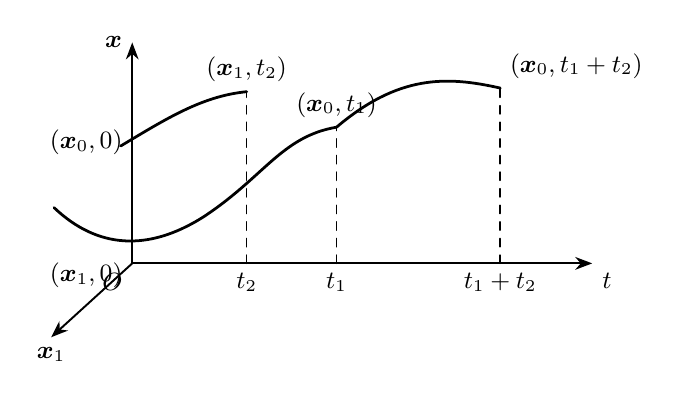
\begin{tikzpicture}[>=Stealth, line cap=round, line join=round,
	font=\small, scale=0.92]
	\coordinate (O) at (0,0);
	\draw[->, line width=0.7pt] (O) -- (6.35,0) node[below right] {$t$};
	\draw[->, line width=0.7pt] (O) -- (0,3.05) node[left] {$\vect{x}$};
	\draw[->, line width=0.7pt] (O) -- (-1.12,-1.02) node[below] {$\vect{x}_1$};
	\node[below left] at (O) {$O$};

	\draw[dashed, line width=0.55pt] (1.58,0) -- (1.58,2.37);
	\draw[dashed, line width=0.55pt] (2.82,0) -- (2.82,1.88);
	\draw[dashed, line width=0.55pt] (5.08,0) -- (5.08,2.42);
	\node[below] at (1.58,0) {$t_2$};
	\node[below] at (2.82,0) {$t_1$};
	\node[below] at (5.08,0) {$t_1+t_2$};

	% 从 $\vect{x}_0$ 出发、在 $t_2$ 时到达 $\vect{x}_1$ 的轨线。
	\draw[line width=1.0pt]
		(-0.16,1.62)
		.. controls (0.46,1.99) and (0.96,2.31) .. (1.58,2.37);
	% 从 $\vect{x}_1$ 出发的轨线；它在 $t_1$ 时到达 $\vect{x}_0$。
	\draw[line width=1.0pt]
		(-1.08,0.77)
		.. controls (-0.48,0.20) and (0.22,0.16) .. (0.98,0.64)
		.. controls (1.82,1.19) and (2.06,1.75) .. (2.82,1.88)
		.. controls (3.67,2.60) and (4.33,2.59) .. (5.08,2.42);

	\node[left] at (0,1.67) {$(\vect{x}_0,0)$};
	\node[below left] at (0,0.14) {$(\vect{x}_1,0)$};
	\node[above] at (1.58,2.37) {$(\vect{x}_1,t_2)$};
	\node[above] at (2.82,1.88) {$(\vect{x}_0,t_1)$};
	\node[above right] at (5.08,2.42) {$(\vect{x}_0,t_1+t_2)$};
\end{tikzpicture}
\captionof{figure}{}
\label{fig:flow-composition}
\end{center}

如今 $f(P, t)$ 表示定常方程 \eqref{eq:3.1} 的当 $t = 0$ 时过点 $P$ 的解. 设 $f(P, t)$ 的定义区间为 $(-\infty, +\infty)$，则对每个固定的 $t$，$f(P, t)$ 定义了开区域 $G \subseteq \R^n$ 到 $G$ 自身的变换，当 $t \in \R$ 时，对 $P \in G$，有 $f(P, t) \in G$. 亦可表示为
\[
f(\cdot, t): G \to G, \quad t \in \R,
\]
或者
\[
f: G \times \R \to G.
\]
而等式 (3.3) 可写成：
\[
f(f(P, t_1), t_2) = f(P, t_1 + t_2).
\]
这说明对单参数变换 $f(\cdot, t)$ 可进行群的运算. 这是定常系统的一个重要性质.

综上所述，如方程 \eqref{eq:3.1} 中的 $F(\vect{x})$ 在 $G \subseteq \R^n$ 上连续，且满足解的唯一性的条件，又设每个解的存在区间为 $(-\infty, +\infty)$，则变换 $f$ 具有下列性质：
\begin{description}
\item[I.] $f(P, 0) = P$;
\item[II.] $f(P, t)$ 对 $P, t$ 一并连续;
\item[III.] $f(f(P, t_1), t_2) = f(P, t_1 + t_2)$.
\end{description}
条件 II 是说，对任何序列 $\{P_n\}, \{t_n\}$，若 $\lim P_n = P$, $\lim t_n = t$，便有 $\lim f(P_n, t_n) = f(P, t)$. 这就是解对初值的连续性和在任何有限的闭的时间区间上对 $t$ 的连续性. 而当 \eqref{eq:3.1} 中的 $F(\vect{x}) \in C^0(G)$ 并满足保证解的唯一性的条件时，便有解对初值与 $t$ 的连续性，故此时性质 II 成立. 性质 I 说 $t = 0$ 对应于恒同变换，它是变换群里的单位元素；由性质 I 和性质 III 立刻推得，对每个变换 $f(\cdot, t_1)$，存在逆变换 $f(\cdot, -t_1)$，满足
\[
f(f(P, t_1), -t_1) = f(P, 0) = P,
\]
因而这些变换组成一个群. 性质 II 说明这些变换对 $(P, t)$ 是连续的，故变换的全体 $\{f(\cdot, t) \mid -\infty < t < +\infty\}$ 组成从 $G$ 到 $G$ 的单参数连续变换群. 这些变换的全体叫做一个动力系统. 有时也把方程 \eqref{eq:3.1} 叫做动力系统.

抽象动力系统是抛开了微分方程，只要 $f$ 是 $G \times \R$ 到 $G$ 的变换，而且满足条件 I, II 和 III，$f$ 就叫做 $G$ 上的一个抽象动力系统，或叫做拓扑动力系统，这是由于对固定的 $t$, $f(\cdot, t)$ 是从 $G$ 到 $G$ 自身的拓扑变换.

在 $G \subseteq \R^n$ 上定义的拓扑动力系统，由条件 II 知道，对固定的 $P \in G$, $\{f(P, t) \mid t \in \R\}$ 是 $G$ 上的一条连续曲线，只是不一定光滑；因此也把 $G$ 上的动力系统叫做 $G$ 上的流. 如果我们还要求 $f$ 是可微的变换，则 $\{f(P, t) \mid t \in \R\}$ 就是 $G$ 上的光滑曲线，在这种情况下 $f$ 就叫做 $G$ 上的微分动力系统，它是近二十年来发展十分活跃的一个新分支. 近年来动力系统的符号和概念被广泛地应用.

\begin{definition}{}{singularity}
若 $\vect{x}_0 \in \R^n$ 满足 $F(\vect{x}_0) = 0$，则 $\vect{x} = \vect{x}_0$ 叫做方程 \eqref{eq:3.1} 的一个奇点.
\end{definition}

由解的唯一性，任何其他解不能在有限时间内到达奇点.

\begin{definition}{}{equivalent}
微分方程组 \eqref{eq:3.1} 与微分方程组
\[
\frac{\dd \vect{x}}{\dd t} = H(\vect{x}) \tag{3.4}\label{eq:3.4}
\]
叫做等价的，如果它们的轨线在相空间 $\R^n$ 的几何图形两两重合（包括奇点），即它们具有相同的轨线.
\end{definition}

\begin{example}{}{equiv1}
方程
\[
\begin{cases}
\dd x/\dd t = y, \\
\dd y/\dd t = -x
\end{cases}
\]
和方程
\[
\begin{cases}
\dd x/\dd t = -y, \\
\dd y/\dd t = x
\end{cases} \tag{3.5}\label{eq:3.5}
\]
在 $\R^2$ 上是等价的.
\end{example}

\begin{example}{}{equiv2}
方程 (3.5) 和方程
\[
\begin{cases}
\dd x/\dd t = y(x^2 + y^2 - 1), \\
\dd y/\dd t = -x(x^2 + y^2 - 1)
\end{cases} \tag{3.6}\label{eq:3.6}
\]
在区域 $x^2 + y^2 \neq 1$ 上是等价的，但在整个 $\R^2$ 上不等价.
\end{example}

\begin{theorem}{}{equiv-system}
设微分方程组 \eqref{eq:3.1} 的右侧函数 $F(\vect{x})$ 在开区域 $D \subseteq \R^n$ 上连续，且满足局部 Lipschitz 条件，则在 $D$ 上存在与 \eqref{eq:3.1} 等价的微分方程组，而它的所有解的存在区间为无限的.
\end{theorem}

\begin{proof}
分两种情形
\begin{enumerate}
\item 若 $D = \R^n$，则取 \eqref{eq:3.1} 的等价系统为
\[
\frac{\dd \vect{x}}{\dd t} = \frac{F(\vect{x})}{\|F(\vect{x})\| + 1}. \tag{3.7}\label{eq:3.7}
\]
因 (3.7) 的右侧函数连续有界，且满足局部 Lipschitz 条件，根据定理~\ref{thm:linear-grow}, (3.7) 的一切解的存在区间均为 $(-\infty, +\infty)$.

\item 若 $D \neq \R^n$，则 $\partial D \neq \emptyset$，且函数 $\rho(\vect{x}, \partial D)$ 在 $D$ 内连续并大于零. 取 \eqref{eq:3.1} 的等价系统为
\[
\frac{\dd \vect{x}}{\dd t} = \frac{\rho(\vect{x}, \partial D) F(\vect{x})}{(\rho(\vect{x}, \partial D) + 1)(\|F(\vect{x})\| + 1)}. \tag{3.8}\label{eq:3.8}
\]
现证 (3.8) 的任一解的存在区间为 $(-\infty, +\infty)$. 用反证法. 若 (3.8) 有解 $\vect{x} = \vect{x}(t, t_0, \vect{x}_0)$，其存在区间右端有界，设为 $[t_0, T]$, $T < +\infty$. 由 (3.8)，
\[
\left\|\frac{\dd \vect{x}(t, t_0, \vect{x}_0)}{\dd t}\right\| < 1,
\]
故轨线弧 $\{\vect{x}(t, t_0, \vect{x}_0) \mid t_0 \leq t < T\}$ 的长度有限，故存在唯一的有极限
\[
\lim_{t \to T-0} \vect{x}(t, t_0, \vect{x}_0) = \vect{y}_0,
\]
显然 $\vect{y}_0 \in \partial D$. 记从 $\vect{x}_0$ 到 $\vect{x}(t, t_0, \vect{x}_0), t_0 \leq t < T$ 的轨线弧的长度为 $s = s(t)$，而从 $\vect{x}_0$ 到 $\vect{y}_0$ 的长度为 $s(T) = s_0$. 由 (3.8) 则有
\[
\frac{\dd s}{\dd t} = \sqrt{\sum_{i=1}^n \left(\frac{\dd x_i}{\dd t}\right)^2} \leq \rho(\vect{x}, \partial D) \leq \rho(\vect{x}, \vect{y}_0) \leq (s_0 - s).
\]
\[
t \geq \int_0^t \frac{\dd s}{s_0 - s} = \ln\frac{s_0}{s_0 - s} \to +\infty, \quad s \to s_0,
\]
从而得矛盾. 因此任一解的存在区间的右端为无界. 同理可证任一解的存在区间的左端也无界.
\end{enumerate}
\end{proof}

以上证明的要点，在于造 \eqref{eq:3.1} 的等价方程 (3.8). (3.8) 可扩充到在 $\bar D$ 上定义，并在其上有界，而在边界 $\partial D$ 上引入奇点. 于是证得 (3.8) 的任何解趋向边界的时间为无限.

为了研究轨线的拓扑结构，由定理~\ref{thm:equiv-system}，我们不妨认为方程 \eqref{eq:3.1} 的解的存在区间无限. 此外，如方程 \eqref{eq:3.1} 的右侧函数 $F(\vect{x})$ 连续，且满足解的唯一性条件，则方程 \eqref{eq:3.1} 的解满足条件 I, II, III，故方程 \eqref{eq:3.1} 是动力系统.

对固定的 $P$, $f(P, t)$ 叫做过 $P$ 点的运动. 集合
\[
f(P, t) = \{f(P, t) \mid -\infty < t < +\infty\}
\]
叫做运动 $f(P, t)$ 的轨线，记成 $L_P$. 集合
\[
f(P, I^+) = \{f(P, t) \mid 0 \leq t < +\infty\}
\]
和集合
\[
f(P, I^-) = \{f(P, t) \mid -\infty < t \leq 0\}
\]
分别叫正半轨线和负半轨线，分别记成 $L_P^+$ 和 $L_P^-$.

\begin{definition}{}{periodic}
若存在 $T > 0$，使得对一切 $t$，有 $f(P, t + T) = f(P, t)$，则 $f(P, t)$ 叫做周期运动.
\end{definition}

由性质 III，这时对一切整数 $n$，有 $f(P, nT + t) = f(P, t)$. 我们称满足等式 $f(P, t + T) = f(P, t)$ 的最小正实数 $T$ 是周期运动 $f(P, t)$ 的周期.

由定义~\ref{def:singularity} 和~\ref{def:periodic}，奇点是周期运动，但它没有最小正周期. 另外，若一周期运动不存在最小正周期，则它必定是奇点. 因这时存在正实数 $T_n \to 0$，使得 $f(P, T_n) = P$. 而对任何实数 $t$，必存在整数 $k_n$，使得 $\lim_{N \to +\infty} \sum_{n=1}^N k_n T_n \to t$. 由性质 II, III，
\[
f(P, t) = \lim_{N \to +\infty} f\left(P, \sum_{n=1}^N k_n T_n\right) = P.
\]
我们把奇点叫做平凡周期运动，非奇点的周期运动叫做非平凡周期运动.

\begin{definition}{}{limit-set}
如果存在时间序列 $t_n \to +\infty (-\infty), n \to +\infty$，使得
\[
\lim_{n \to +\infty} f(P, t_n) = q,
\]
则点 $q$ 叫做 $f(P, t)$ 的 $\omega(\alpha)$ 极限点. $f(P, t)$ 的所有 $\omega(\alpha)$ 极限点的全体记作 $\Omega_P(A_P)$.
\end{definition}

由定义~\ref{def:periodic}，若 $f(P, t)$ 是周期运动，则对任意固定的 $t$, $f(P, nT + t) = f(P, t)$，其中 $T$ 是周期，$n$ 是任何整数. 再令 $n \to +\infty$ 或 $-\infty$，我们便推出 $\Omega_P = A_P = L_P$. 特别来说，若 $P$ 是奇点，则 $\Omega_P = A_P = P$.

\begin{definition}{}{invariant}
如果对一切 $t \in (-\infty, +\infty)$，集合 $A$ 满足 $f(A, t) = A$，其中 $f(A, t) = \{f(P, t) \mid P \in A\}$，则 $A$ 叫做 $f$ 的不变集合.
\end{definition}

易知任何一条轨线是不变集合. 由定义知道不变集合是由整条整条的轨线组成的.

\begin{theorem}{}{omega-invariant}
对一切 $t \in (-\infty, +\infty)$，必有 $f(\Omega_P, t) = \Omega_P$，即 $\Omega_P$ 是不变集合.
\end{theorem}

\begin{proof}
设 $q \in \Omega_P$, $r = f(q, t)$. 要证 $r \in \Omega_P$. 因 $q \in \Omega_P$，根据定义，存在 $t_n \to +\infty$, $n \to +\infty$,
\[
\lim_{n \to +\infty} f(P, t_n) = q.
\]
由动力系统性质 II 和 III，
\[
\lim_{n \to +\infty} f(P, t_n + t) = \lim_{n \to +\infty} f(f(P, t_n), t) = f(q, t) = r,
\]
即 $r \in \Omega_P$，这就证明了 $f(\Omega_P, t) \subset \Omega_P$. 对一切 $t \in (-\infty, +\infty)$，又由性质 II 和 III，对一切 $t \in (-\infty, +\infty)$，有 $f(f(\Omega_P, t), -t) \subset f(\Omega_P, -t)$，即 $\Omega_P \subset f(\Omega_P, -t)$. 这就证明了，对一切 $t \in (-\infty, +\infty)$ 有 $f(\Omega_P, t) = \Omega_P$.
\end{proof}

\begin{theorem}{}{omega-closed}
$\Omega_P$ 是闭集.
\end{theorem}

\begin{proof}
如 $P_n \in \Omega_P$ 和 $\lim_{n \to +\infty} P_n = q$，要证 $q \in \Omega_P$. 任给 $\varepsilon > 0$, $\exists m > 0$, $\rho(P_m, q) < \varepsilon/2$. 因 $P_m \in \Omega_P$，故 $\exists t_m > 0$，使 $\rho(P_m, f(P, t_m)) < \varepsilon/2$. 从而 $\rho(q, f(P, t_m)) < \varepsilon$，故 $q \in \Omega_P$.
\end{proof}

\begin{definition}{}{connected}
如果不存在对集合 $M$ 而言的闭子集 $M_1, M_2 \subset M$，使得 $M_1 \cap M_2 = \emptyset$ 和 $M = M_1 \cup M_2$，则集合 $M$ 叫做连通的，否则叫做不连通.
\end{definition}

设 $M_1, M_2$ 是 $M$ 的闭子集，且 $M = M_1 \cup M_2$ 和 $M_1 \cap M_2 = \emptyset$. 因 $M_2 = M \setminus M_1$，因而 $M_1$ 和 $M_2$ 又是 $M$ 的开子集. $M_1, M_2$ 便足 $M$ 的开闭子集. $M$ 和空集 $\emptyset$ 叫做 $M$ 的平凡开闭子集. 如果 $M$ 无非平凡开闭子集，则 $M$ 是连通的. 如果 $M$ 有非平凡开闭子集，则 $M$ 不连通，它的每个开闭子集是它的一个连通分支.

\fuzhu{2}{定义~\ref{def:connected} 叫区域连通，它与曲线连通有区别. 请读者举出区域连通非曲线连通的例子.}

\begin{theorem}{}{omega-connected}
如果 $f(P, I^+)$ 有界，则 $\Omega_P$ 连通.
\end{theorem}

\begin{proof}
设 $\Omega_P$ 不连通，则 $\exists \Omega_P^{(1)}, \Omega_P^{(2)} \subset \Omega_P$, $\Omega_P = \Omega_P^{(1)} \cup \Omega_P^{(2)}$, $\Omega_P^{(1)} \cap \Omega_P^{(2)} = \emptyset$, $\Omega_P^{(1)}, \Omega_P^{(2)}$ 是对 $\Omega_P$ 而言的闭集. 因 $\Omega_P$ 是对 $\R^n$ 而言的闭集，因而 $\Omega_P^{(1)}, \Omega_P^{(2)}$ 也是对 $\R^n$ 而言的闭集. 故 $\rho(\Omega_P^{(1)}, \Omega_P^{(2)}) = d > 0$. 故存在序列 $t_n^{(i)} \to +\infty$, $f(P, t_n^{(i)}) \in S(\Omega_P^{(i)}, d/3)$, $i = 1, 2$. 并且
\[
0 < t_1^{(1)} < t_1^{(2)} < t_2^{(1)} < t_2^{(2)} < \cdots < t_n^{(1)} < t_n^{(2)} < \cdots.
\]
\[
\rho\left[S\left(\Omega_P^{(1)}, \frac{d}{3}\right), S\left(\Omega_P^{(2)}, \frac{d}{3}\right)\right] > \frac{d}{3}.
\]
可取 $t_n^{(i)} < \xi_n < t_n^{(2)}$, $f(P, \xi_n) \in S(\Omega_P^{(1)}, d/3) \cup S(\Omega_P^{(2)}, d/3)$. 由于 $f(P, I^+)$ 有界，在 $\{f(P, \xi_n)\}$ 中可选出收敛子序列. 为简单起见，就设原序列收敛，即 $\lim_{n \to +\infty} f(P, \xi_n) = q \in \Omega_P$. 导出矛盾，故 $\Omega_P$ 连通.
\end{proof}

定理~\ref{thm:omega-invariant}, \ref{thm:omega-closed}, \ref{thm:omega-connected} 对 $A_P$ 也相应地成立.

按 $\Omega_P(A_P)$ 的性质，可将动力系统 \eqref{eq:3.1} 的轨线分成三大类：
\begin{enumerate}
\item 如果 $\Omega_P(A_P)$ 为空集，则 $f(P, t)$ 叫做正（负）向远离轨线；既正向又负向远离的轨线叫做远离轨线.
\item 如果 $\Omega_P(A_P)$ 非空，但 $\Omega_P \cap f(P, I^+) = \emptyset$ ($A_P \cap f(P, I^-) = \emptyset$)，则 $f(P, t)$ 叫做正（负）向渐近轨线；既正向又负向的渐近轨线叫做渐近轨线.
\item 如果 $\Omega_P \cap f(P, I^+) \neq \emptyset$ ($A_P \cap f(P, I^-) \neq \emptyset$)，则 $f(P, t)$ 叫做正（负）向 Poisson 稳定轨线，简称 $P^+(P^-)$ 稳定轨线；既正向又负向 Poisson 稳定轨道叫做 Poisson 稳定轨线，或简称 $P$ 式稳定轨线.
\end{enumerate}

\begin{example}{}{saddle}
给定微分方程
\[
\frac{\dd x}{\dd t} = x, \quad \frac{\dd y}{\dd t} = -y,
\]
其图形如图~1.3.
\end{example}

\begin{center}
	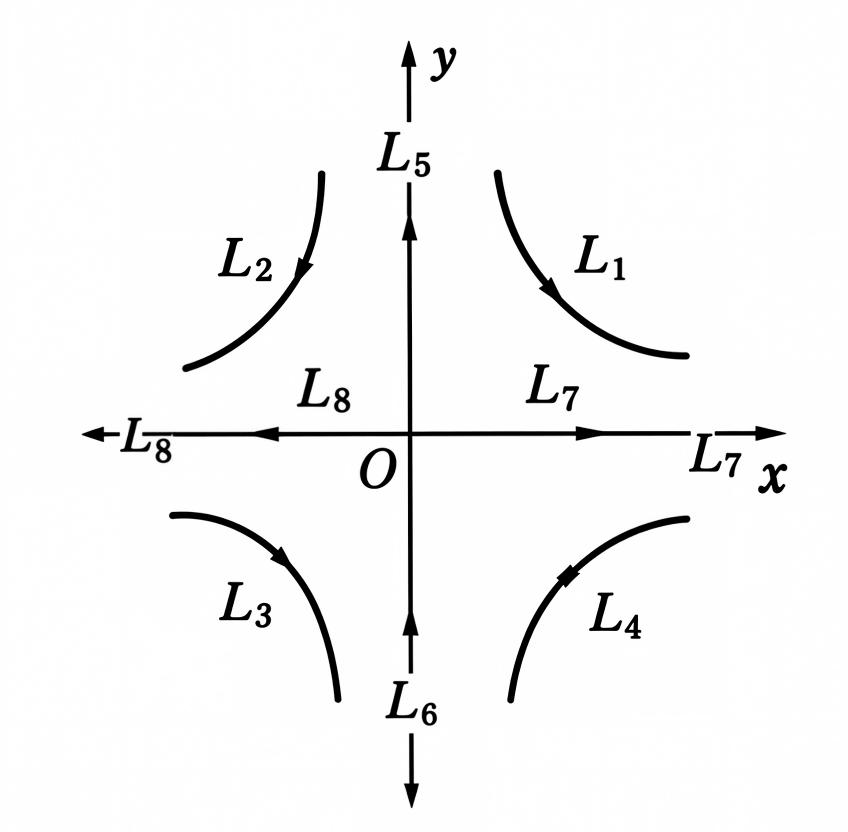
\includegraphics[width=0.5\linewidth]{figure/1.3}
	\captionof{figure}{}
\end{center}
对上图，$L_1, L_2, L_3, L_4$ —— 远离轨线；$L_5, L_6$ —— 正向渐近, 负向远离轨线；$L_7, L_8$ —— 负向渐近, 正向远离轨线；$O$ —— $P$ 稳定轨线.

\begin{center}
	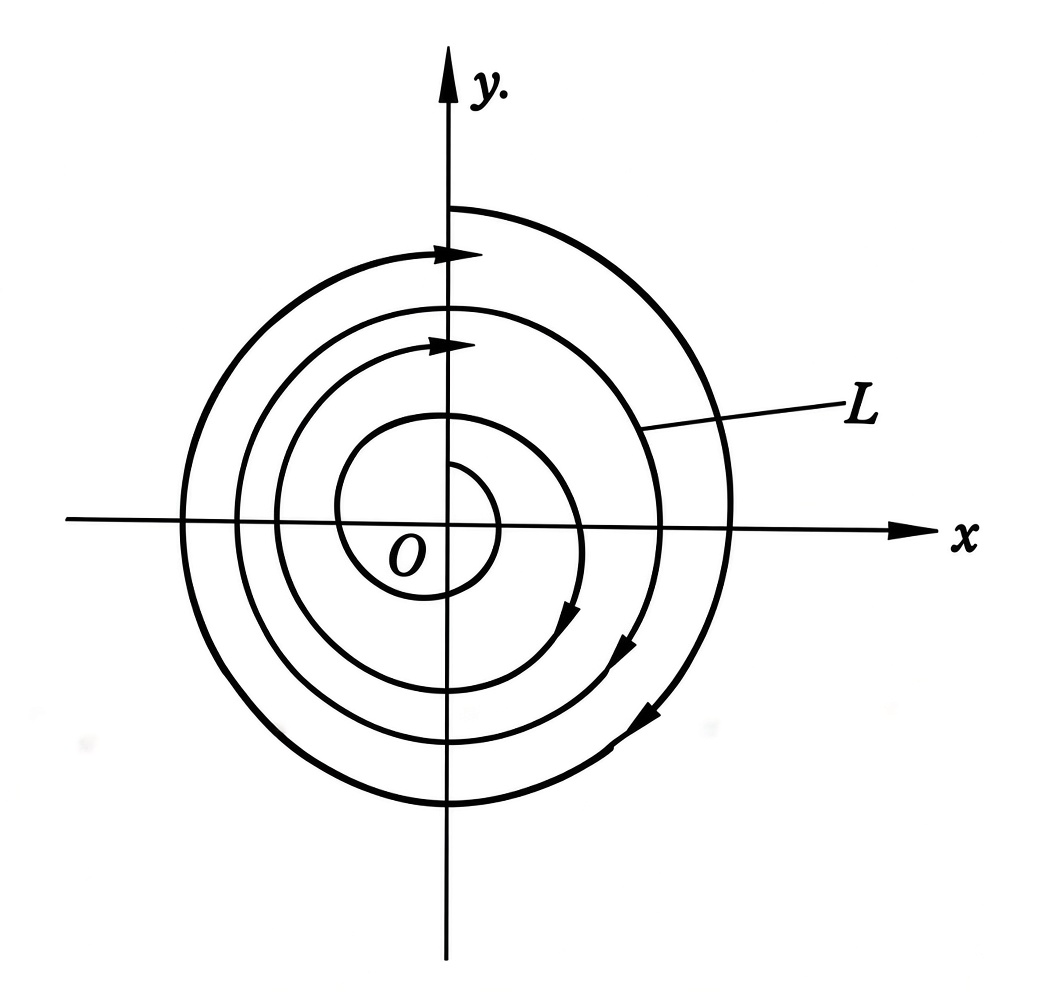
\includegraphics[width=0.5\linewidth]{figure/1.4}
	\captionof{figure}{}
\end{center}
原点 $O$ 和闭轨线 $L$ ($r = 1$) —— $P$ 式稳定轨线；$L_r(0 < r < 1)$ —— 渐近轨线；$L_r(r > 1)$ —— 正向渐近, 负向远离轨线.

\begin{example}{}{lim-cycle}
给定微分方程
\[
\begin{aligned}
\frac{\dd x}{\dd t} &= y + x[1 - (x^2 + y^2)], \\
\frac{\dd y}{\dd t} &= -x + y[1 - (x^2 + y^2)].
\end{aligned}
\]
令 $x = r\cos\theta, y = r\sin\theta$，原方程化为
\[
\frac{\dd r}{\dd t} = r(1 - r^2), \quad \frac{\dd \theta}{\dd t} = -1,
\]
或者
\[
\frac{\dd r}{\dd \theta} = r(r^2 - 1).
\]
易知 $r = 0, r = 1$ 都是轨线，而且 $\dd \theta/\dd t < 0$ 和 $(r - 1) \dd r/\dd \theta > 0$. 故在相平面 $(x, y)$ 上的图形如图~1.4.
\end{example}

% ============================================================
%  §4  平面上的动力系统
% ============================================================
\sourceSection{平面上的动力系统}

给定微分方程组
\[
\begin{cases}
\dd x/\dd t = X(x, y), \\
\dd y/\dd t = Y(x, y),
\end{cases} \tag{4.1}\label{eq:4.1}
\]
其中 $X(x, y), Y(x, y)$ 是定义在 $\R^2$ 上的连续函数，并且满足条件，以保证初值问题的解唯一. 由定理~\ref{thm:equiv-system}，可认为 \eqref{eq:4.1} 的每个解的存在区间为 $(-\infty, +\infty)$，故 \eqref{eq:4.1} 在 $\R^2$ 上定义了一个动力系统.

\textbf{Jordan 定理}\quad 任何 $\R^2$ 上的单闭曲线 $L$ 将 $\R^2$ 分成两部分 $-D_1$ 和 $D_2$，且 $D_1$ 内任何一点到 $D_2$ 内任何一点的连续路径必与 $L$ 相交.

这一节的结果基本是由解的存在唯一性和 Jordan 定理这个简单的几何事实推得的，其中主要结果是由 H. Poincaré 和 I. Bendixson 得到的. 另外必须指出有些结论只是在底空间是欧氏平面 $\R^2$ 或者二维球面 $S^2$ 时才成立，这主要是因为 Jordan 定理的缘故.

\begin{theorem}{}{closed-sing}
方程 \eqref{eq:4.1} 的所有奇点组成闭集.
\end{theorem}

\begin{proof}
要证，如果 $(x_n, y_n)$ 是奇点，且当 $n \to +\infty$ 时 $(x_n, y_n) \to (\bar x, \bar y)$，则 $(\bar x, \bar y)$ 也是奇点. 由 $X^2(x_n, y_n) + Y^2(x_n, y_n) = 0$，便知
\[
\lim_{n \to +\infty} \left[X^2(x_n, y_n) + Y^2(x_n, y_n)\right] = X^2(\bar x, \bar y) + Y^2(\bar x, \bar y) = 0.
\]
\end{proof}

\begin{definition}{}{non-tangent}
$\overline{N_1N_2}$ 为直线. 如果凡是与 $\overline{N_1N_2}$ 相交的轨线，当 $t$ 增加时只能从 $\overline{N_1N_2}$ 的同一侧到另一侧，而且没有轨线与 $\overline{N_1N_2}$ 相切，则 $\overline{N_1N_2}$ 叫做无切线段.
\end{definition}

\begin{lemma}{}{flow-box}
设 $P_0$ 是 \eqref{eq:4.1} 的常点，则存在过 $P_0$ 的无切线段 $\overline{N_1N_2}$，以及曲边长方形 $ABCD$, $AB \parallel \overline{N_1N_2} \parallel DC$, $AD, BC$ 为轨线段，自 $ABCD$ 内任一点出发的轨线，当它向两侧延续时，必分别与 $AB$ 和 $CD$ 各相交一次（从一侧穿过 $\overline{N_1N_2}$）.
\end{lemma}

\begin{proof}
取 $\varepsilon > 0$ 充分小，使 $\overline{S(P_0, \varepsilon)}$ 中不包含奇点. 作过 $P_0(x_0, y_0)$ 点的轨线的法线段 $\overline{N_1N_2}$，其方程为：
\[
Y(x_0, y_0)(y - y_0) + X(x_0, y_0)(x - x_0) = 0.
\]
令
\[
\lambda(x, y) = Y(x_0, y_0)(y - y_0) + X(x_0, y_0)(x - x_0) = C,
\]
它是一组平行于 $\overline{N_1N_2}$ 的直线族. 对这组平行直线族沿着方程组 \eqref{eq:4.1} 所定义的向量场求方向导数，得
\[
\frac{\dd \lambda}{\dd t} = Y(x_0, y_0) Y(x, y) + X(x_0, y_0) X(x, y).
\]
因 $\dd\lambda/\dd t|_{(x_0, y_0)} = Y^2(x_0, y_0) + X^2(x_0, y_0) > 0$，由连续性，存在 $0 < \delta \leq \varepsilon$，使得当 $(x, y) \in S(P_0, \delta)$ 时，也有 $\dd\lambda/\dd t > 0$. 这就是说，\eqref{eq:4.1} 的轨线在 $S(P_0, \delta)$ 中当 $t$ 增加时沿着 $C$ 增加的方向与平行直线族相交. 如图~1.5 所示，取 $\overline{N_1N_2} \subset S(P_0, \delta)$，$\overline{N_1N_2}$ 就是无切线段. 显然，可以作满足引理要求的曲边长方形 $ABCD \subset S(P_0, \delta)$，将它记为 $\square \overline{N_1N_2}$.
\end{proof}

\begin{center}
	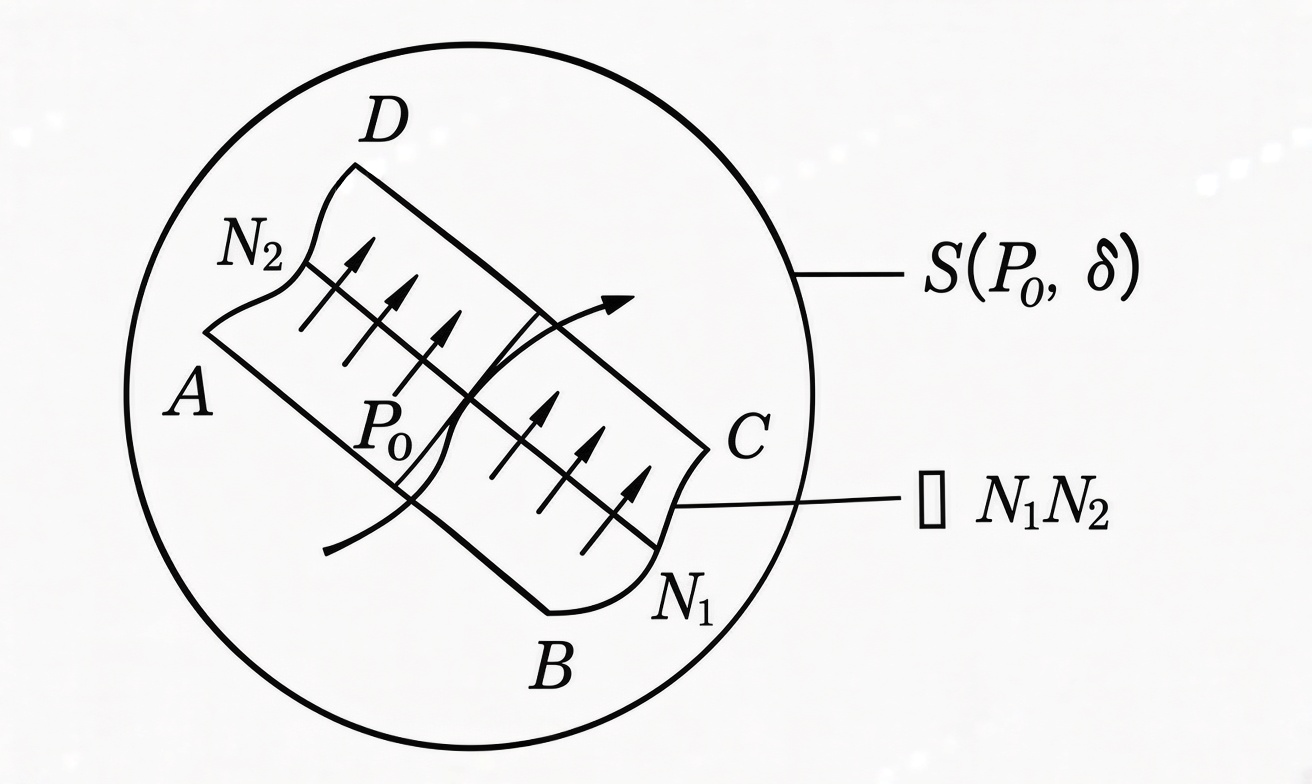
\includegraphics[width=0.5\linewidth]{figure/1.5}
	\captionof{figure}{}
\end{center}


在 $\R^n$ 上定义的一个连续向量场，它在 $\R^n$ 上决定一个连续流；在任何常点 $P$ 附近，也能作出具有类似上述性质的曲边长方体，它叫做过 $P$ 点的流盒. 沿用这个名词，我们也将满足引理~\ref{lem:flow-box} 的曲边长方形叫做过 $P$ 点的流盒.

\begin{lemma}{}{order}
设 $\overline{N_1N_2}$ 为无切线段，$\square \overline{N_1N_2}$ 为满足引理~\ref{lem:flow-box} 的流盒，又设 $f(P, I^+)$（或 $f(P, I^-)$）与 $\overline{N_1N_2}$ 按时间次序相交于 $M_1, M_2, M_3$，则 $M_2$ 必落在 $M_1$ 与 $M_3$ 之间.
\end{lemma}

\begin{proof}
只证括号外的. $f(P, I^+)$ 与 $\overline{N_1N_2}$ 相交于 $M_2$ 之后不能离开（或进入）由轨线段 $M_1SM_2$ 与无切线段 $M_1M_2$ 所围成的区域 $D$，如上图中 (1)（或图 (2)）所示. 因根据解的唯一性，$f(P, I^+)$ 不能与 $M_1SM_2$ 相交，也不能经过 $M_1M_2$ 离开（或进入）$D$. 既然 $f(P, I^+)$ 自 $M_2$ 之后永远停留在 $D$ 内（或外），$M_3$ 就不能落在 $M_1, M_2$ 之间，而 $M_2$ 必落在 $M_1$ 与 $M_3$ 之间. 这时我们简称 $f(P, I^+)$ 按次序与无切线段 $\overline{N_1N_2}$ 相交于 $M_1, M_2, M_3$.
\end{proof}

\begin{theorem}{}{poincare}
设 $f(P, I)$ 是 $P^+$（或 $P^-$）稳定轨线，则 $f(P, I)$ 是奇点或闭轨线.
\end{theorem}
\begin{center}
	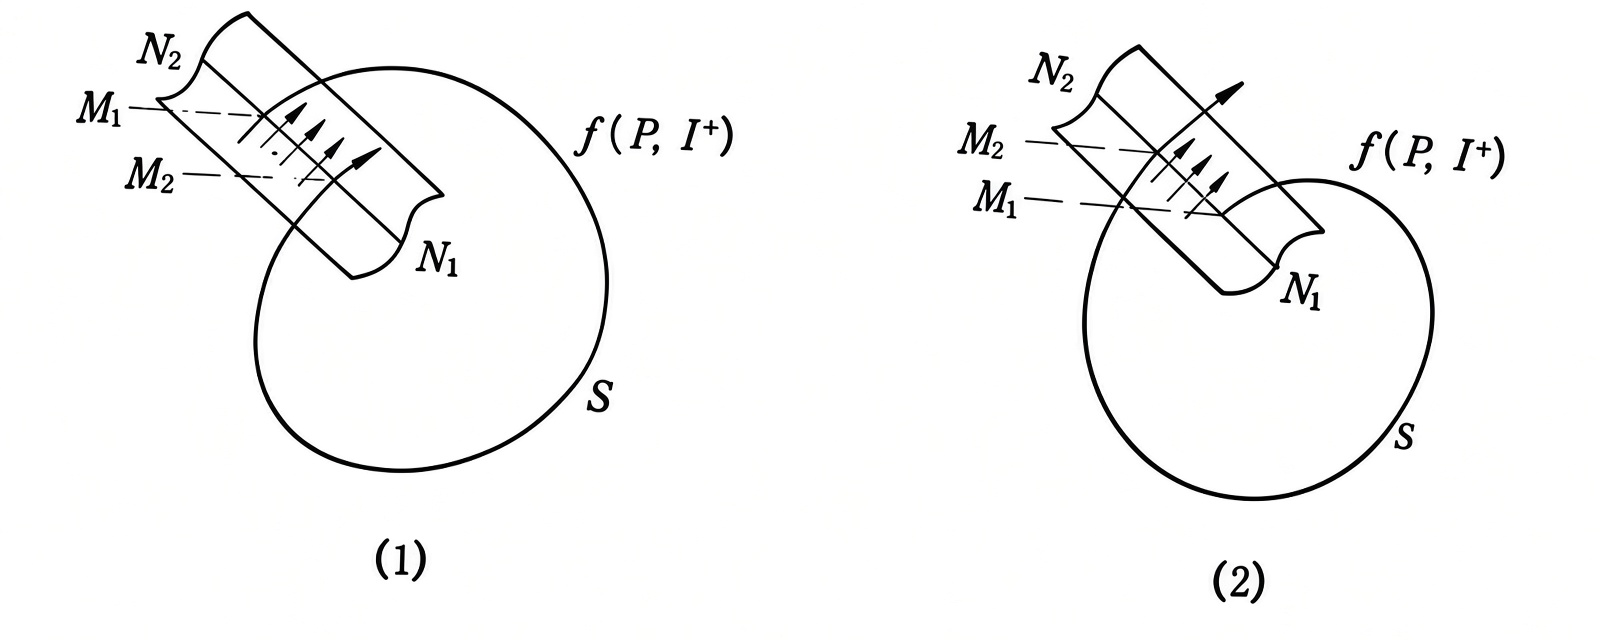
\includegraphics[width=0.7\linewidth]{figure/1.6}
	\captionof{figure}{}
\end{center}

\begin{proof}
只证正向的情形. 因 $\Omega_P \cap f(P, I^+) \neq \emptyset$，取 $M_1 \in \Omega_P \cap f(P, I^+)$. 如 $M_1$ 是奇点，则 $f(P, I^+) = \Omega_P = M_1$，定理得证. 如 $M_1$ 不是奇点，过 $M_1$ 作流盒 $\square \overline{N_1N_2}$. 因 $M_1 \in \Omega_P$，必存在 $T > 0$, $f(P, I^+)$ 离开 $\square \overline{N_1N_2}$ 后，在时刻 $T$ 时，再次进入 $\square \overline{N_1N_2}$，即 $f(P, T) \in \square \overline{N_1N_2}$. 根据 $\square \overline{N_1N_2}$ 的性质，$f(P, I^+)$ 在 $T$ 附近向正向或负向延续时，与 $\overline{N_1N_2}$ 相交于 $M_2$，其图形只能是下列三种情形之一：图~1.6 中的 (1), (2) 或下图~1.7. 如发生图~1.6 中的情形 (1) 或 (2)，由引理~\ref{lem:order}, $f(P, I^+)$ 自 $M_2$ 之后不可能再回到 $M_1$ 的任意小邻域. 故 $M_1 \in \Omega_P$，得矛盾. 故只能是图~1.7 的情形，即 $f(P, I) = L_P$ 是闭轨线.
\end{proof}


\begin{corollary}{}{pplus-pp}
平面上的 $P^+$ 或 $P^-$ 稳定轨线必为 $P$ 式稳定轨线.
\end{corollary}

本定理说明，在 $\R^2$ 上的 $P$ 式稳定轨线只能是奇点或闭轨线. 但当底空间不是 $\R^2$ 时，一般来说，$P$ 式稳定轨线可以是非常复杂的，它不属于本节讨论的范围.
\begin{center}
	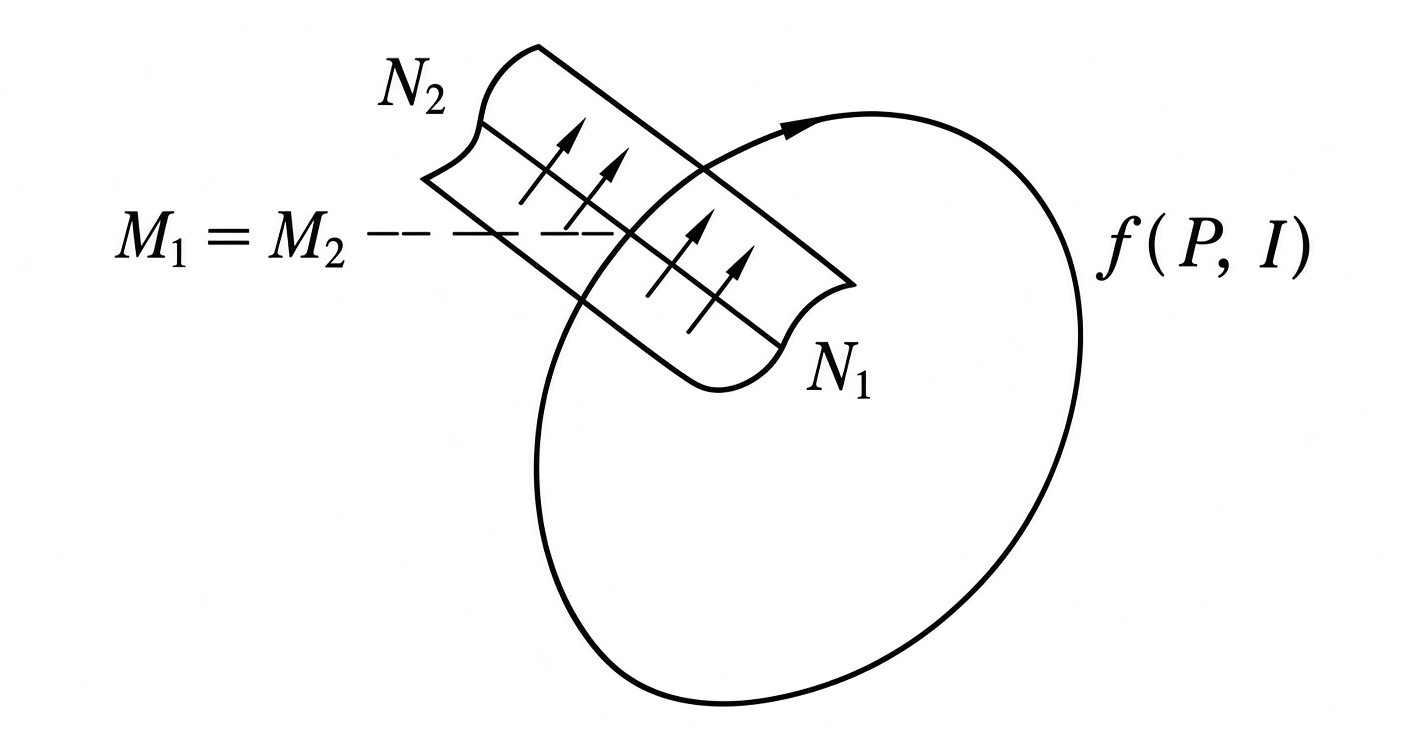
\includegraphics[width=0.7\linewidth]{figure/1.7}
	\captionof{figure}{}
\end{center}

\begin{theorem}{}{omega-L}
如 $L$ 为闭轨线，$L \subset \Omega_P(A_P)$，则 $\Omega_P = L$ ($A_P = L$).
\end{theorem}

\begin{proof}
只证括号外的. 要证，对任意小的 $\varepsilon_1 > 0$，存在充分大的实数 $r > 0$, $f(P, t) \subset S(L, \varepsilon_1)$，当 $t > r$ 时，这就证明了 $\Omega_P = L$. 如图~1.8 所示，在 $L$ 上取一点 $Q$，过 $Q$ 作流盒 $\square \overline{N_1N_2} \subset S(Q, \varepsilon_1)$. 取 $\varepsilon_2$ 充分小，使 $S(Q, \varepsilon_2) \subset \square \overline{N_1N_2}$. 设 $T$ 为 $L$ 的周期. 根据解对初值的连续性，对 $\varepsilon_2$ 与 $T$，存在正数 $\delta(\varepsilon_2, T) < \varepsilon_2$，当 $\rho(Q, R) < \delta$ 和 $0 \leq t \leq T$，就有 $\rho(f(Q, t), f(R, t)) < \varepsilon_2$. 因 $Q \in \Omega_P$，存在 $f(P, t_1) = M_1 \in S(Q, \delta) \cap \overline{N_1N_2}$，故有 $\rho(f(P, t_1 + t), f(Q, t)) < \varepsilon_2$, $0 \leq t \leq T$，即 $\rho(f(P, t_1 + T), Q) < \varepsilon_2$，即 $f(P, t_1 + T) \in S(Q, \varepsilon_2) \subset \square \overline{N_1N_2}$. 由 $\square \overline{N_1N_2}$ 的性质，当 $f(P, t_1 + T)$ 向正向或负向延长时必与 $\overline{N_1N_2}$ 相交，设交点为 $M_2$. 由引理~\ref{lem:order}, $M_2$ 必落在 $M_1$ 与 $Q$ 之间. 否则 $Q$ 将不属于 $\Omega_P$，故 $\rho(M_2, Q) < \delta$. 再由 $\delta$ 的定义及 $\square \overline{N_1N_2}$ 的性质，$f(P, t)$ 自 $M_2$ 之后都落在 $S(L, \varepsilon_2)$ 中. 因 $\varepsilon_1$ 为任给，故 $\Omega_P = L$.
\end{proof}
\begin{center}
	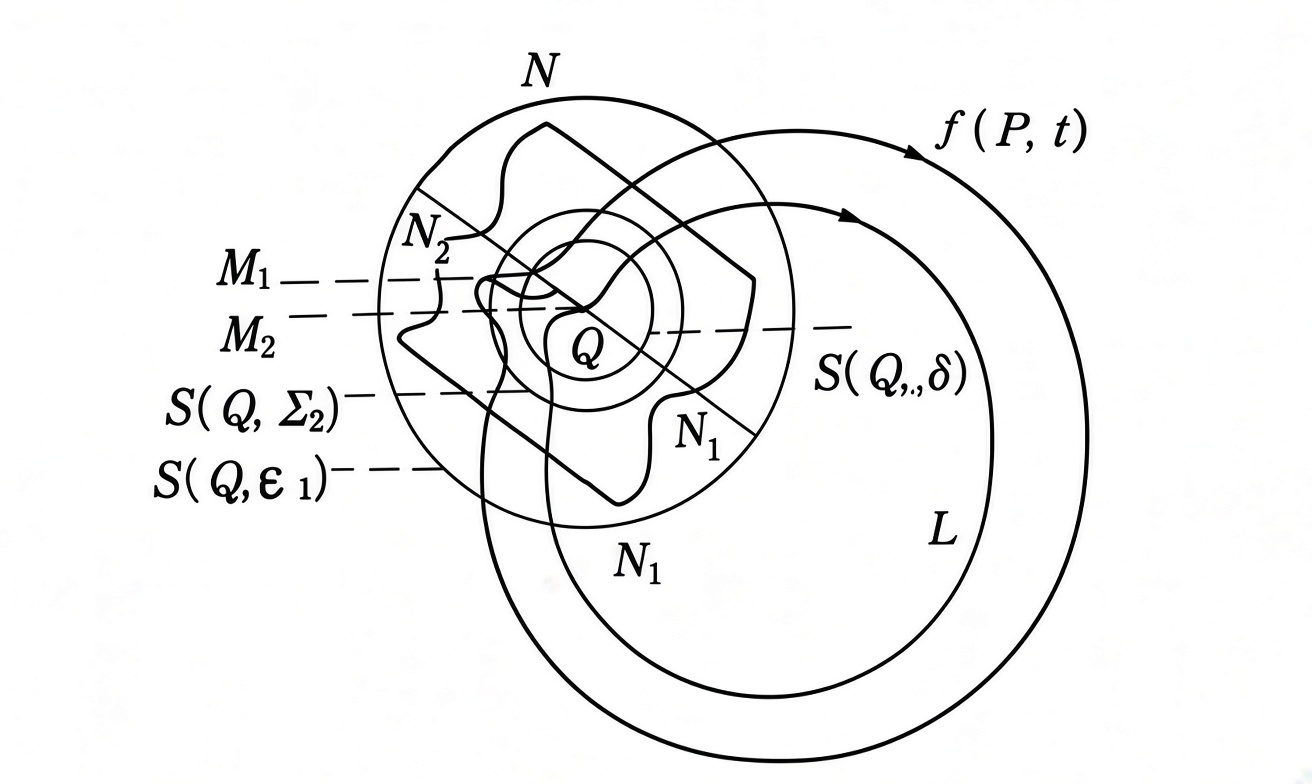
\includegraphics[width=0.7\linewidth]{figure/1.8}
	\captionof{figure}{}
\end{center}



\begin{theorem}{}{omega-bounded}
若 $\Omega_P(A_P)$ 有界非空，且不包含奇点，则 $\Omega_P(A_P)$ 必为闭轨线.
\end{theorem}

\begin{proof}
只证括号外的. 若 $f(P, I)$ 为 $P^+$ 稳定轨线，则由定理~\ref{thm:poincare}, $f(P, I) = \Omega_P$ 为闭轨线，本定理成立. 若 $f(P, I)$ 非 $P^+$ 稳定轨线，即 $f(P, I^+) \cap \Omega_P = \emptyset$. 则可用反证法. 设 $\Omega_P$ 非闭轨线，取 $Q \in \Omega_P$，因 $\Omega_P$ 有界，故 $\Omega_P$ 非空，且 $\Omega_P \subset \Omega_P$，根据定理~\ref{thm:omega-L}, $\Omega_P$ 非闭轨线，否则 $\Omega_P = L$ 将为闭轨线. $\Omega_P$ 非奇点又非闭轨线，由定理~\ref{thm:poincare}, $f(Q, I^+)$ 非 $P^+$ 稳定，即 $f(Q, I^+) \cap \Omega_P = \emptyset$. 取 $B \in \Omega_P$，因 $B$ 非奇点，过 $B$ 作流盒 $\square \overline{N_1N_2}$. 因 $B \in f(Q, I^+)$，故存在时间序列 $t_1 < t_2 < t_3$, $M_i = f(Q, t_i) \in \overline{N_1N_2}$, $i = 1, 2, 3$.
\[
\rho(M_1, B) > \rho(M_2, B) > \rho(M_3, B) > 0.
\]
取 $\delta > 0$ 充分小，使得
\[
S(M_i, \delta) \cap S(M_j, \delta) = \emptyset, \quad i, j = 1, 2, 3, i \neq j.
\]
\[
S(M_i, \delta) \subset \square \overline{N_1N_2}, \quad i = 1, 2, 3.
\]
因 $M_3 \in \Omega_P$，由 $\square \overline{N_1N_2}$ 的性质，存在 $R = f(P, T) \in \overline{N_1N_2} \cap S(M_3, \delta)$. 根据图~1.9 (1)（或 (2)），当 $t > T$, $f(P, t)$ 将不可能进入（或离开）由轨线弧 $M_3SM_3$ 及无切线段 $M_1M_3$ 所围成的区域，因此不可能进入 $S(M_1, \delta)$. 故 $M_1 \in \Omega_P$，得矛盾，这就否定了反证法的前提，定理得证.
\end{proof}
\begin{center}
	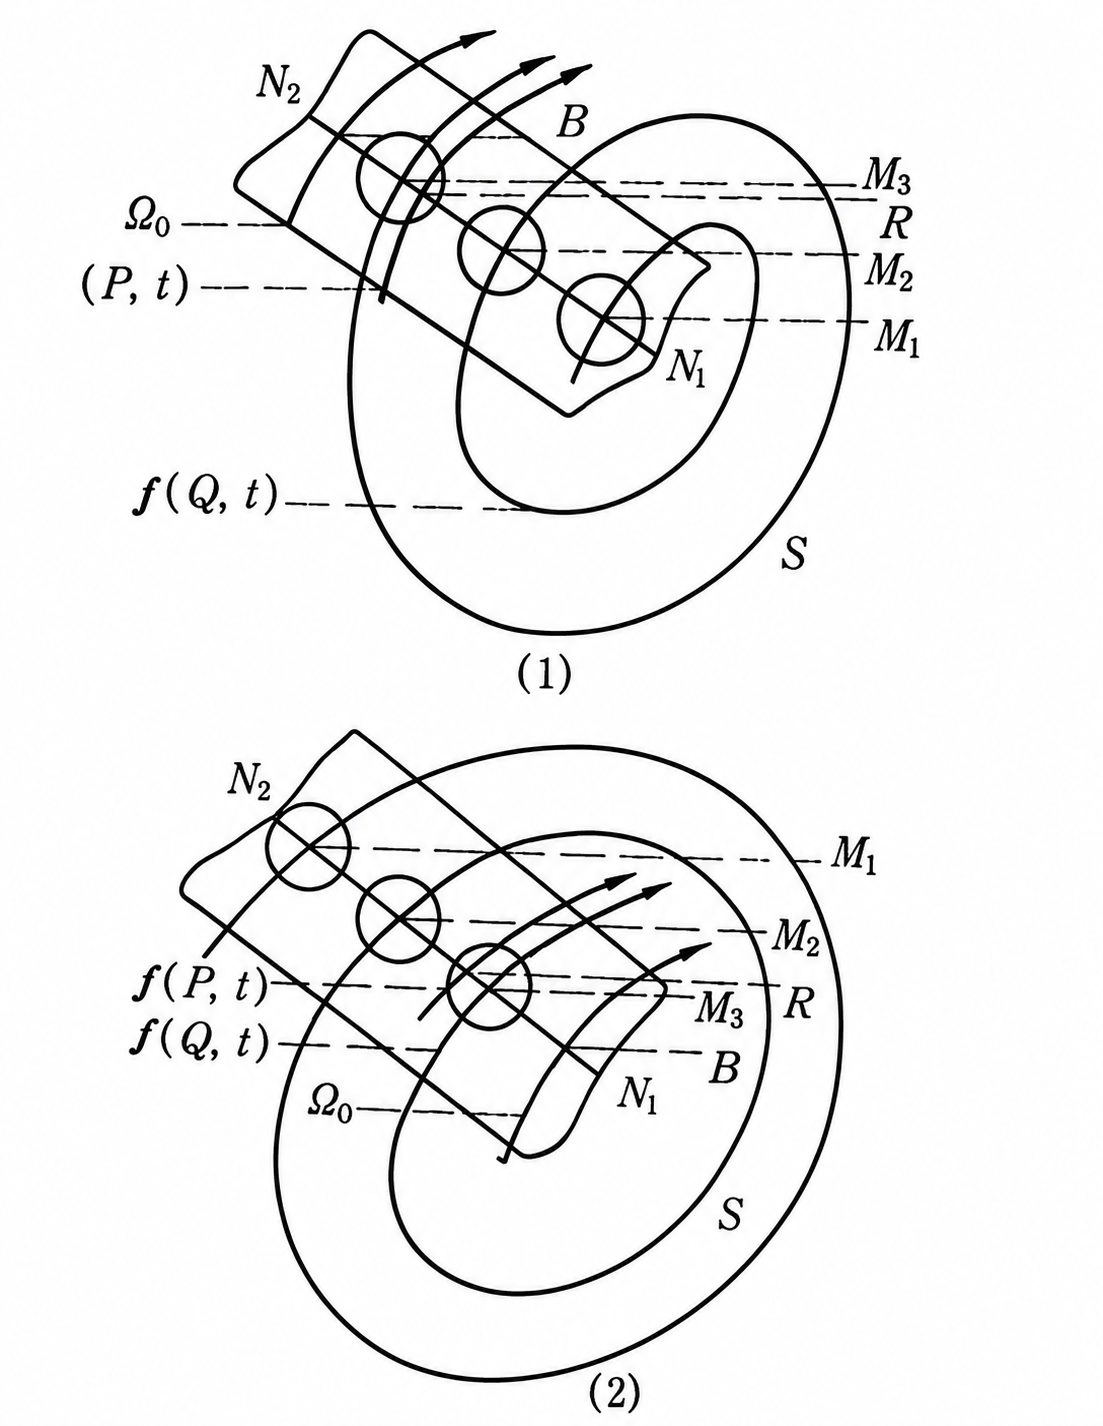
\includegraphics[width=0.5\linewidth]{figure/1.9}
	\captionof{figure}{}
\end{center}


注意，定理中关于 $\Omega_P$ 有界的条件是不可缺少的，否则 $\Omega_P$ 可以既不包含奇点，也非闭轨线. 请看下图.
\begin{center}
	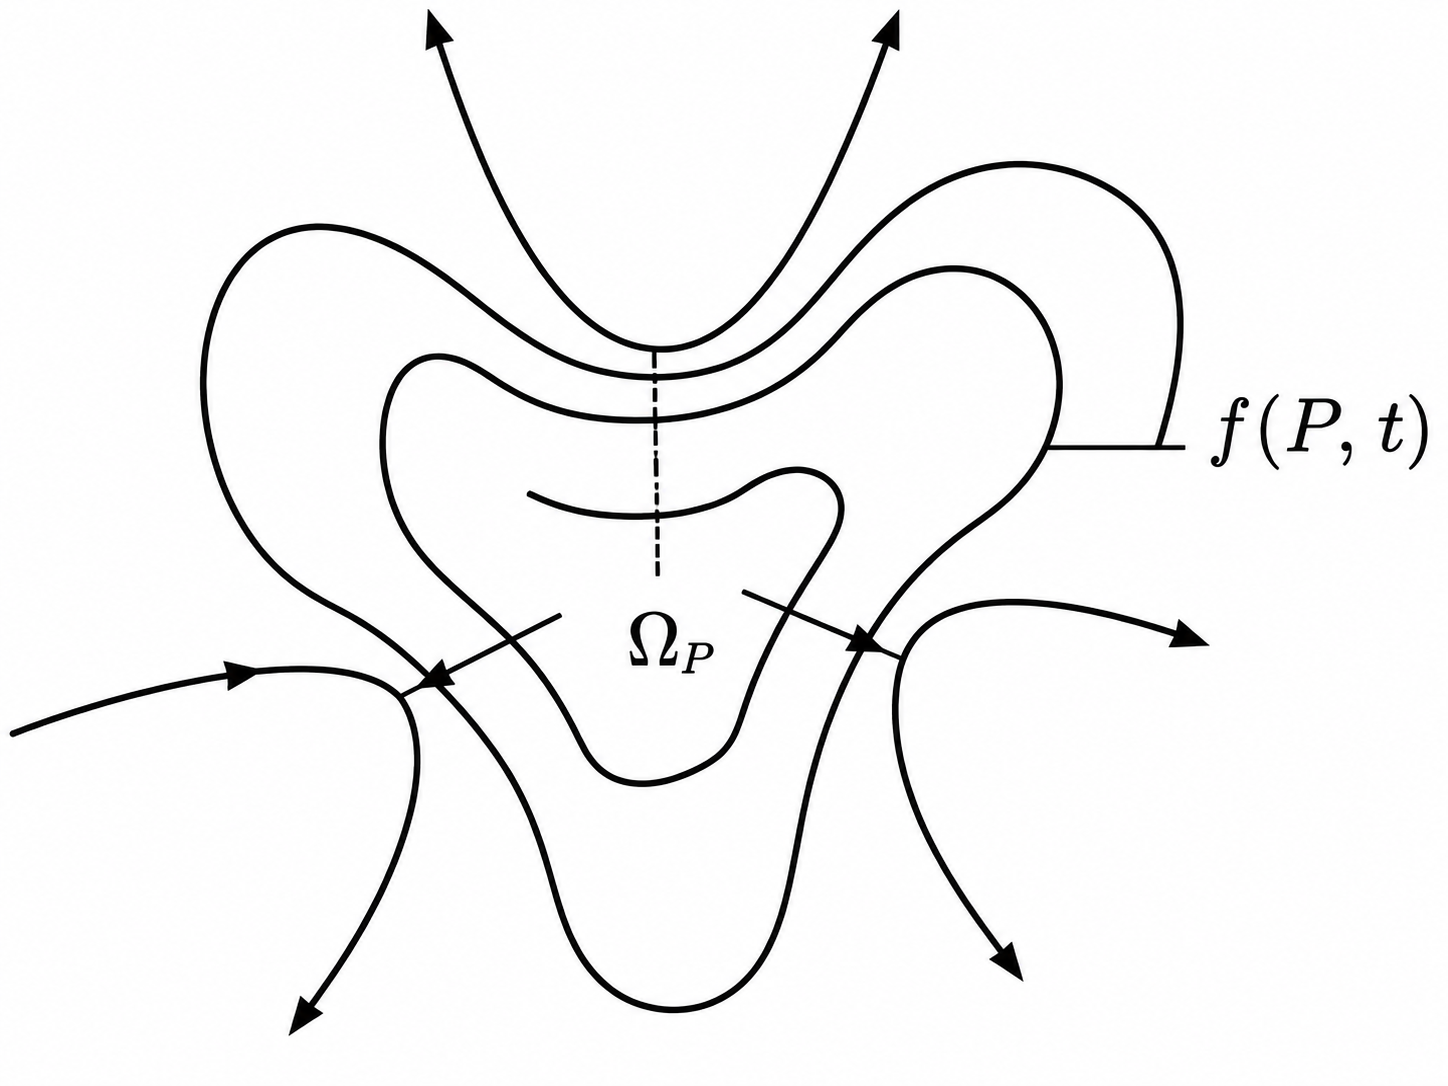
\includegraphics[width=0.5\linewidth]{figure/1.10}
	\captionof{figure}{}
\end{center}
\newpage


\begin{theorem}{}{omega-neighbor}
若 $f(P, I)$ 非闭轨线，$\Omega_P$ 为闭轨线，则存在 $S(P, \varepsilon)$，对任何 $Q \in S(P, \varepsilon)$，必有 $\Omega_Q = \Omega_P$.
\end{theorem}

由定理~\ref{thm:omega-bounded} 及解对初值的连续依赖性便可证明.

\begin{corollary}{}{ap-omega}
若 $f(P, I)$ 非闭轨线，$\Omega_P$ 为闭轨线，则 $A_P \cap \Omega_P = \emptyset$.
\end{corollary}

\begin{theorem}{}{sing-inside}
在平面上任何闭轨线 $L$ 所包围的区域中必有奇点.
\end{theorem}

\begin{proof}
令 $L$ 所包围的区域为 $D$. 假设 $D$ 中无奇点. 任取 $P_1 \in D$，由定理~\ref{thm:omega-bounded}, $\Omega_{P_1}$ 和 $A_{P_1}$ 均为闭轨线. 由定理~\ref{thm:omega-neighbor} 的推论，或者 $L_{P_1} = \Omega_{P_1} = A_{P_1}$ 是闭轨线，或者 $\Omega_{P_1} \neq A_{P_1}$，也即在 $D$ 中必有异于 $L$ 的闭轨线 $L_1 \subset L$（符号 $L_1 \subset L$ 的意思是 $L_1 \subset D$）. 同样可证存在异于 $L_1$ 的闭轨线 $L_2 \subset L_1 \subset L$. 对任意点 $Q(x, y) \in D$，定义函数
\[
F(x, y) = \begin{cases}
d, & \text{当 } f(Q, I) \text{ 非闭轨线}, d \text{ 为 } D \text{ 的面积}, \\
a(x, y), & \text{当 } f(Q, I) \text{ 是闭轨线}, a(x, y) \text{ 是 } f(Q, I) \text{ 所包围的面积}.
\end{cases}
\]
$F(x, y) > 0$ 为 $D$ 上的单值函数，故 $F(x, y)$ 在 $D$ 上有下确界 $C < d$，因 $F(x, y)$ 不一定连续，故 $F(x, y)$ 不一定达到下确界，但必存在 $(x_n, y_n) \in D$，使 $F(x_n, y_n) \to C$. 因 $(x_n, y_n)$ 有界，必有收敛子序列. 为符号简单起见，就设 $(x_n, y_n) \to (x_0, y_0)$, $A(x_0, y_0) \in D$. 考虑轨线 $f(A, I)$. 设 $f(A, I)$ 非闭轨线，由定理~\ref{thm:omega-bounded}, $\Omega_A$ 为闭轨线. 由定理~\ref{thm:omega-neighbor}，存在 $S(A, \varepsilon) \subset D$，对任何 $B \in S(A, \varepsilon)$, $f(B, I)$ 非闭轨线. 且 $\Omega_B = \Omega_A$. 故由定理定义，$F(x, y) = d$，当 $(x, y) \in S(A, \varepsilon)$，得矛盾. 故 $f(A, I) = L_A$ 为闭轨线. 于是存在闭轨线 $L'$ 和 $L''$, $L'' \subset L' \subset L_A$. 对充分小的 $\varepsilon > 0$ 及 $Q(x, y) \in S(A, \varepsilon)$，考虑 $f(Q, I)$. 如果 $f(Q, I)$ 为闭轨线，则 $L'' \subset L' \subset L_Q = f(Q, I)$. 设 $d'$ 和 $d''$ 分别是 $L'$ 和 $L''$ 所包围的区域的面积，则 $F(x, y) > d' > d''$；如果 $L_A$ 非闭轨线，则按定义 $F(x, y) = d$，故对一切 $(x_n, y_n) \in S(A, \varepsilon)$, $F(x_n, y_n) > d' > d''$. $\lim F(x_n, y_n) = C \geq d' > d''$. 这与 $F(x, y)$ 在 $D$ 上的下确界为 $C$ 相矛盾. 因而 $L_A$ 既不能是闭轨线，也不能是非闭轨线. 这就推翻了 $D$ 中无奇点的假设，定理得证.
\end{proof}

本定理也可用超限归纳法来证明，请参看文献~\cite{petrovskii-stepanov-1949} 中第二章.

\begin{theorem}{(Poincaré-Bendixson 环域定理)}{poincare-bendixson}
设 $D$ 是由两条单闭曲线 $L_1$ 和 $L_2$ 所包围成的环域，并且在 $D$ 内无奇点；又设当 $t$ 增加时从 $L_1, L_2$ 上出发的轨线都进入（或都离开）$D$，则在 $D$ 内存在闭轨线 $L$，其相对位置是 $L_1 \subset L \subset L_2$.
\end{theorem}

\begin{proof}
由定理~\ref{thm:omega-bounded}，在 $D$ 内有闭轨线 $L$. 由定理~\ref{thm:sing-inside}，其相对位置必为 $L_1 \subset L \subset L_2$.
\end{proof}

本定理的条件可减弱成：$\bar D$ 上无奇点，从 $L_1$ 和 $L_2$ 上出发的轨线都不能离开（或都不能进入）$\bar D$，但 $L_1$ 和 $L_2$ 上均有奇点，从它出发的轨线进入（或离开）$D$，则 $D$ 内有闭轨线. 换句话说，环域 $D$ 的内外境界线 $L_1$ 和 $L_2$ 都可以包含轨线弧.

以下讨论闭轨线附近轨线的分布情形.

\begin{theorem}{}{closed-nearby}
设 $L$ 为闭轨线，则对充分小 $\varepsilon > 0$，存在相应适当小 $\delta > 0$，对任何 $Q \in S(L, \delta)$，至少 $f(Q, I^+), f(Q, I^-)$ 之一落在 $S(L, \varepsilon)$ 中，并且与过 $L$ 上每一点的无切线段按同一顺序相交（顺时针或逆时针）.
\end{theorem}

\begin{proof}
对任何 $P \in L$，作法线 $\overline{N_1N_2}(P)$. 对任何充分小实数 $\varepsilon_1 > 0$，使 $S(L, \varepsilon_1)$ 中无奇点，并作流盒 $\square \overline{N_1N_2}(P) \subset S(P, \varepsilon_1)$. 令 $\square N_1N_2(P)$ 表示流盒 $\square \overline{N_1N_2}(P)$ 的内点集，它是开集. 由 $L$ 的紧致性，必存在有限个 $\square N_1N_2(P_k)$ 将 $L$ 覆盖住. 即
\[
\bigcup_{k=1}^n \square N_1N_2(P_k) \supset L.
\]
于是便存在充分小 $\varepsilon_2 > 0$，有
\[
S(L, \varepsilon_2) \subset \bigcup_{k=1}^n \square N_1N_2(P_k).
\]
设点 $P_1, P_2, \cdots, P_k, \cdots, P_n, P_1$ 按顺序两两相邻地排列在 $L$ 上. 设 $T$ 为 $L$ 的周期. 由解对初值的连续依赖性，$\exists \delta(\varepsilon_2, T) > 0$，对任何点 $P \in L$，当 $Q \in S(P, \delta)$，与定理~\ref{thm:omega-L} 相类似，可证至少 $f(Q, I^+)$ 和 $f(Q, I^-)$ 之一落在 $S(L, \varepsilon_2)$ 中. 由 $L$ 的紧致性，可使这里的 $\delta$ 与 $P$ 无关. 设 $f(Q, I^+)$ 落在 $S(L, \varepsilon_2)$ 中，由向量场的连续性，$f(Q, I^+)$ 将按顺序与流盒 $\bigcup_{k=1}^n [\square N_1N_2(P_k)]$ 相交. $L_Q$ 可为闭轨线. 若 $L_Q$ 非闭轨线，而 $\Omega_Q = L$ 或 $A_Q = L$，我们就相应地称半轨 $L_Q^+$ 或 $L_Q^-$ 绕 $L$ 盘旋.
\end{proof}

\begin{theorem}{}{annulus}
设 $D$ 是由两条闭轨线 $L_1 \subset L_2$ 所围成的环域，$D$ 中无奇点也无其他闭轨线，则对一切 $Q \in D$，必有 $\Omega_Q = L_1$, $A_Q = L_2$（或者 $\Omega_Q = L_2$, $A_Q = L_1$）.
\end{theorem}

从定理~\ref{thm:omega-bounded} 和~\ref{thm:omega-neighbor} 的推论可立刻推得.

设 $L$ 为闭轨线，$P \in L$，过 $P$ 作无切线段 $\overline{R_1PR_2}$, $\rho(R_1, P) = \rho(P, R_2) = \delta$，其中 $\delta$ 满足定理~\ref{thm:closed-nearby} 的要求，设 $R_1$ 落在 $L$ 之外. 令 $F = \{Q \mid Q \in \overline{R_1P}, f(Q, I) \text{ 为闭轨}\}$，现证 $F$ 为闭集. 用反证法. 设 $F$ 非闭集，则必存在 $Q_n \in F, Q_n \to B \in F$，即 $f(B, I)$ 非闭轨. 由定理~\ref{thm:closed-nearby}, $f(B, I^+)$ 和 $f(B, I^-)$ 之一必停留在 $S(L, \varepsilon_1)$ 中，$\varepsilon_1$ 和 $\delta$ 的取法如定理~\ref{thm:closed-nearby}. 由定理~\ref{thm:omega-bounded}, $\Omega_B$ 或 $A_B$ 是闭轨线. 由定理~\ref{thm:omega-neighbor}, $\exists \eta > 0$，对一切 $R \in S(B, \eta)$, $\Omega_B = \Omega_R$ 或 $A_B = A_R$，但 $f(R, I)$ 非闭轨线. 这与 $Q_n \in F, Q_n \to B$ 相矛盾，故 $F$ 是闭集. 于是下列两种情况必居其一：
\begin{enumerate}
\item $P$ 为 $F$ 的孤立点. 这时存在充分小的 $0 < \xi < \eta$，任何 $R \in \overline{R_1P} \cap S(L, \xi)$, $f(R, I)$ 的正半轨或负半轨落在 $S(L, \varepsilon_1)$ 中，并绕 $L$ 盘旋，相应地有 $\Omega_R = L$ 或 $A_R = L$.
\item $P$ 为 $F$ 的聚点. 这时从 $\overline{R_1P} \cap S(L, \xi)$ 出发的轨线，或者都是闭轨线，或者其中既有异于 $L$ 的闭轨线又有非闭轨线.
\end{enumerate}
对 $\overline{PR_2}$ 上的点也可进行类似的讨论.

\begin{definition}{}{limit-cycle}
设 $L$ 是闭轨线. 如果存在 $S(L, \varepsilon)$，对任何 $Q \in S(L, \varepsilon)$，有 $\Omega_Q = L$（这时 $f(Q, I^+)$ 绕 $L$ 盘旋），或者有 $A_Q = L$（这时 $f(Q, I^-)$ 绕 $L$ 盘旋），则 $L$ 叫做极限环.
\end{definition}

由以上讨论知，闭轨线附近轨线分布必为下列五种情形之一：
\begin{enumerate}
\item 稳定极限环. $\exists S(L, \varepsilon)$，对任何 $Q \in S(L, \varepsilon)$，有 $\Omega_Q = L$.
\item 不稳定极限环. $\exists S(L, \varepsilon)$，对任何 $Q \in S(L, \varepsilon)$，有 $A_Q = L$.
\item 半稳定极限环. $\exists S(L, \varepsilon)$，对任何 $Q \in S(L, \varepsilon)$，当 $Q$ 落在 $L$ 的一侧，$\Omega_Q = L$，当 $Q$ 落在 $L$ 的另一侧，$A_Q = L$.
\item 周期环域. $\exists S(L, \varepsilon)$，对任何 $Q \in S(L, \varepsilon)$, $f(Q, I)$ 是闭轨线.
\item 复型极限环. 对任意 $\varepsilon > 0$, $S(L, \varepsilon)$ 中既有异于 $L$ 的闭轨线，又有非闭轨线.
\end{enumerate}
往后我们将证明，对解析向量场，即 \eqref{eq:4.1} 的右侧是解析函数时，第 5 种情形不可能发生.

以下进一步讨论 $\Omega_P(A_P)$ 的构造.

先讨论 $\Omega_P$ 有界的情形.

设 $\Omega_P = \Omega_P^{(1)} \cup \Omega_P^{(2)}$, $\Omega_P^{(1)}$ 为常点集，$\Omega_P^{(2)}$ 为奇点集，已证 $\Omega_P^{(2)}$ 是闭集. $\Omega_P^{(2)} = \bigcup_\alpha C_\alpha$, $C_\alpha \cap C_\beta = \emptyset$，当 $\alpha \neq \beta$, $C_\alpha$ 是 $\Omega_P^{(2)}$ 的连通分支.

\begin{definition}{}{touch}
对任何点 $Q$，如果 $\Omega_Q \subset C_\alpha$（或 $A_Q \subset C_\alpha$），轨线 $f(Q, I)$ 就叫做正向（或负向）接触 $C_\alpha$.
\end{definition}

\begin{theorem}{}{countable}
考虑轨线 $f(P, I)$，设 $\Omega_P$ 有界，$\Omega_P = \Omega_P^{(1)} \cup \Omega_P^{(2)}$, $\Omega_P^{(1)} \neq \emptyset$, $\Omega_P^{(2)} \neq \emptyset$，则 $\Omega_P^{(1)}$ 中的每一条轨线都正向和负向接触 $\Omega_P^{(2)}$ 中的一个连通分支，同时 $\Omega_P^{(1)}$ 由可列条轨线组成.
\end{theorem}

\begin{proof}
因 $\Omega_P^{(1)} \neq \emptyset$, $\Omega_P^{(2)} \neq \emptyset$，由定理~\ref{thm:omega-L}, $\Omega_P^{(1)}$ 中无闭轨线. 设 $R \in \Omega_P^{(1)}$，因 $\Omega_P$ 是闭集，故 $\Omega_R \subset \Omega_P$, $\Omega_R \neq \emptyset$. 与定理~\ref{thm:omega-bounded} 类似的步骤，可证 $\Omega_R$ 中无奇点（见习题~9）. $\Omega_R$ 有界，由定理~\ref{thm:omega-connected}, $\Omega_R$ 连通，故 $\Omega_R \subset C_\alpha$. 同样可证 $A_R \subset C_\beta$（也可能 $C_\alpha = C_\beta$）. 定理的前半部分已证明了. 再证 $\Omega_P^{(1)}$ 由可列条轨线组成.

取 $A \in \Omega_P^{(1)}$，因 $A$ 为常点，过 $A$ 作流盒 $\square \overline{N_1N_2}$，由 $\square \overline{N_1N_2}$ 的性质，$f(P, I)$ 只能交 $\overline{N_1N_2}$ 于 $A$ 的一侧，设交于 $\overline{AN_2}$，并且 $f(P, I)$ 与 $\overline{AN_2}$ 只能按次序相交于 $M_1, M_2, M_3, \cdots, M_n, \cdots$，且 $M_n \to A$. 因此在 $\square N_1N_2$ 中除了 $A_1AA_2 = f(A, I) \cap \square N_1N_2$ 外，再没有 $\Omega_P$ 的其他的点. 取正整数 $m$ 适当大，使 $S(A, 1/m) \subset \square N_1N_2$. 对 $\Omega_P^{(1)}$ 中每条轨线都作相应的圆 $S(A, 1/m)$，这些圆 $S(A, 1/m)$ 互不包含别的圆的圆心. 因 $\Omega_P$ 有界，可使 $\Omega_P^{(1)} \subset G \subset \R^2$，其中 $G$ 为有界区域. 对固定的整数 $m > 0$, $G$ 上互不包含彼此圆心的圆 $S(A, 1/m)$ 的个数为有限个，不同的半径 $1/m$ 最多是可列个，因而 $G$ 上这样的圆 $S(A, 1/m)$ 的个数最多是可列个. 故 $\Omega_P^{(1)}$ 最多由可列条轨线组成.
\end{proof}

\begin{corollary}{}{cor1-4-10}
如果 $\Omega_P$ 有界，$\Omega_P = \Omega_P^{(1)} \cup \Omega_P^{(2)}$, $\Omega_P^{(1)}$ 非空，$\Omega_P^{(2)}$ 只包含一个奇点 $O$，则 $\Omega_P^{(1)}$ 中最多有可列条轨线，每条轨线都正向和负向接触于 $O$，如图~1.11 所示.
\end{corollary}
\begin{center}
	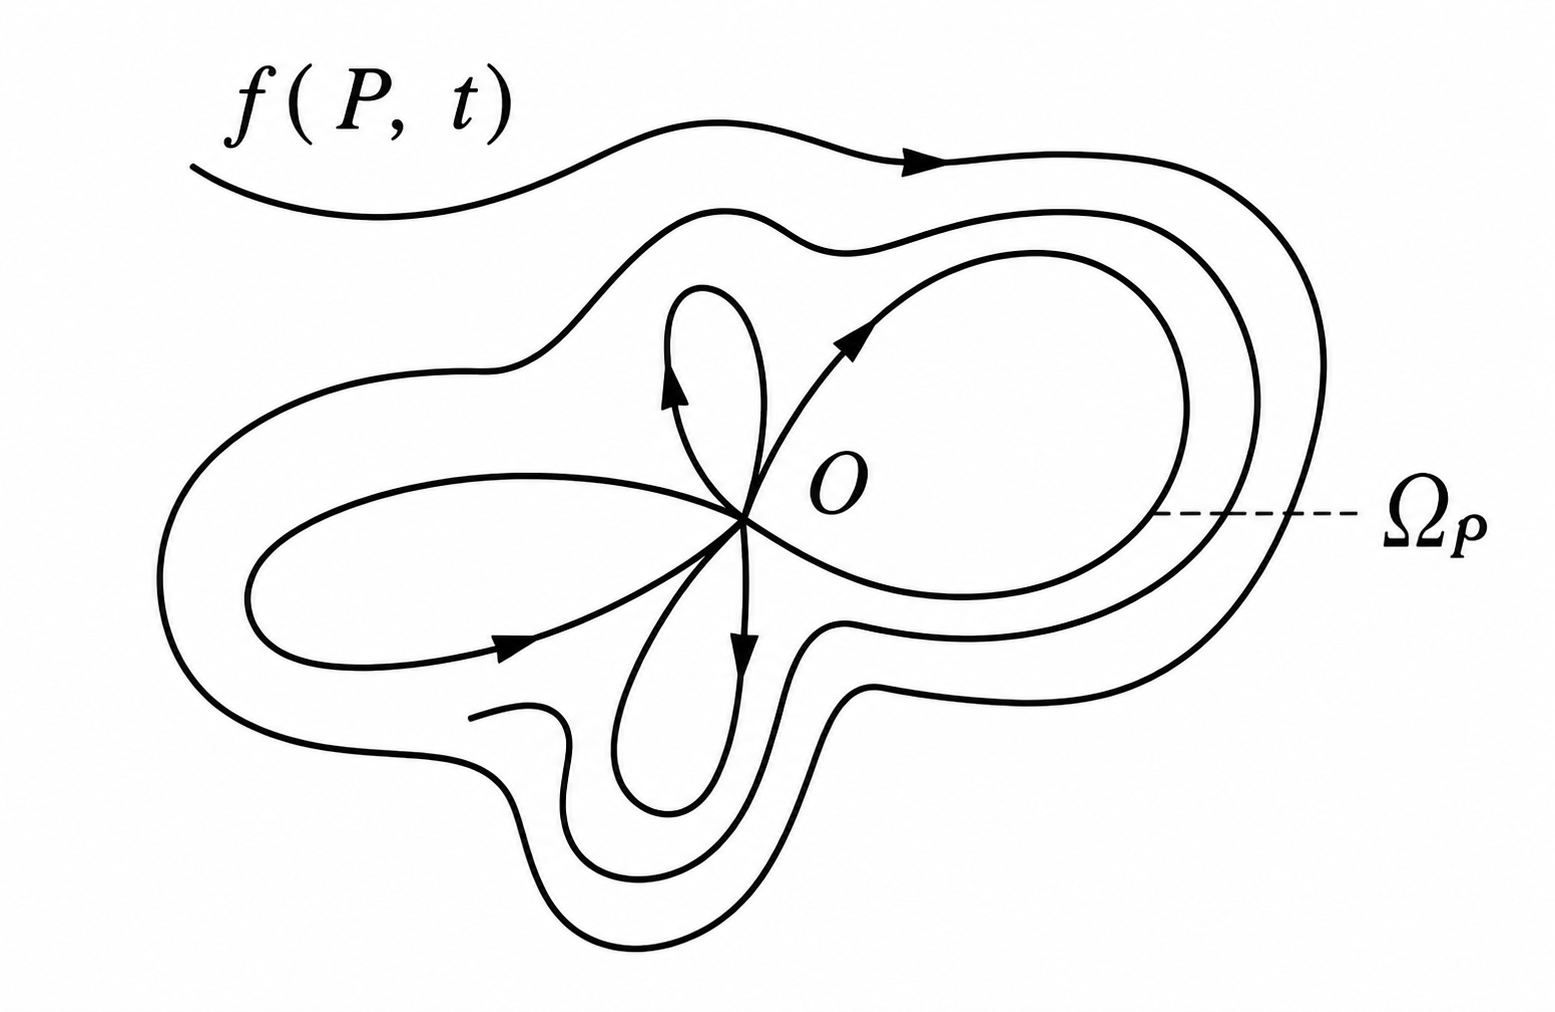
\includegraphics[width=0.5\linewidth]{figure/1.11}
	\captionof{figure}{}
\end{center}


\begin{corollary}{}{cor2-4-10}
$G$ 为有界区域，$G$ 中有唯一的奇点 $O$. 如果 $f(P, I^+) \subset G$，则 $f(P, I^+)$ 必为下列五种情形之一：
\begin{enumerate}
\item[(1)] $P = \{O\}$.
\item[(2)] $\Omega_P = \{O\}, f(P, I^+) \cap \Omega_P = \emptyset$.
\item[(3)] $f(P, I) = \Omega_P$ 为闭轨线，奇点 $O$ 属于 $\Omega_P$ 所包围的区域.
\item[(4)] $\Omega_P$ 为闭轨线，$f(P, I^+) \cap \Omega_P = \emptyset$，奇点 $O$ 属于 $\Omega_P$ 所包围的区域.
\item[(5)] $\Omega_P = \Omega_P^{(1)} \cup \Omega_P^{(2)}, \Omega_P^{(2)} = \{O\}, \Omega_P^{(1)} \neq \emptyset$. 

它们的图形分别如图~1.12 中 (1), (2), (3), (4), (5) 所示. 图形 (4) 中也可能 $f(P, I)$ 落在闭轨线 $\Omega_P$ 所包围的区域中.
\end{enumerate}
\end{corollary}

\begin{center}
	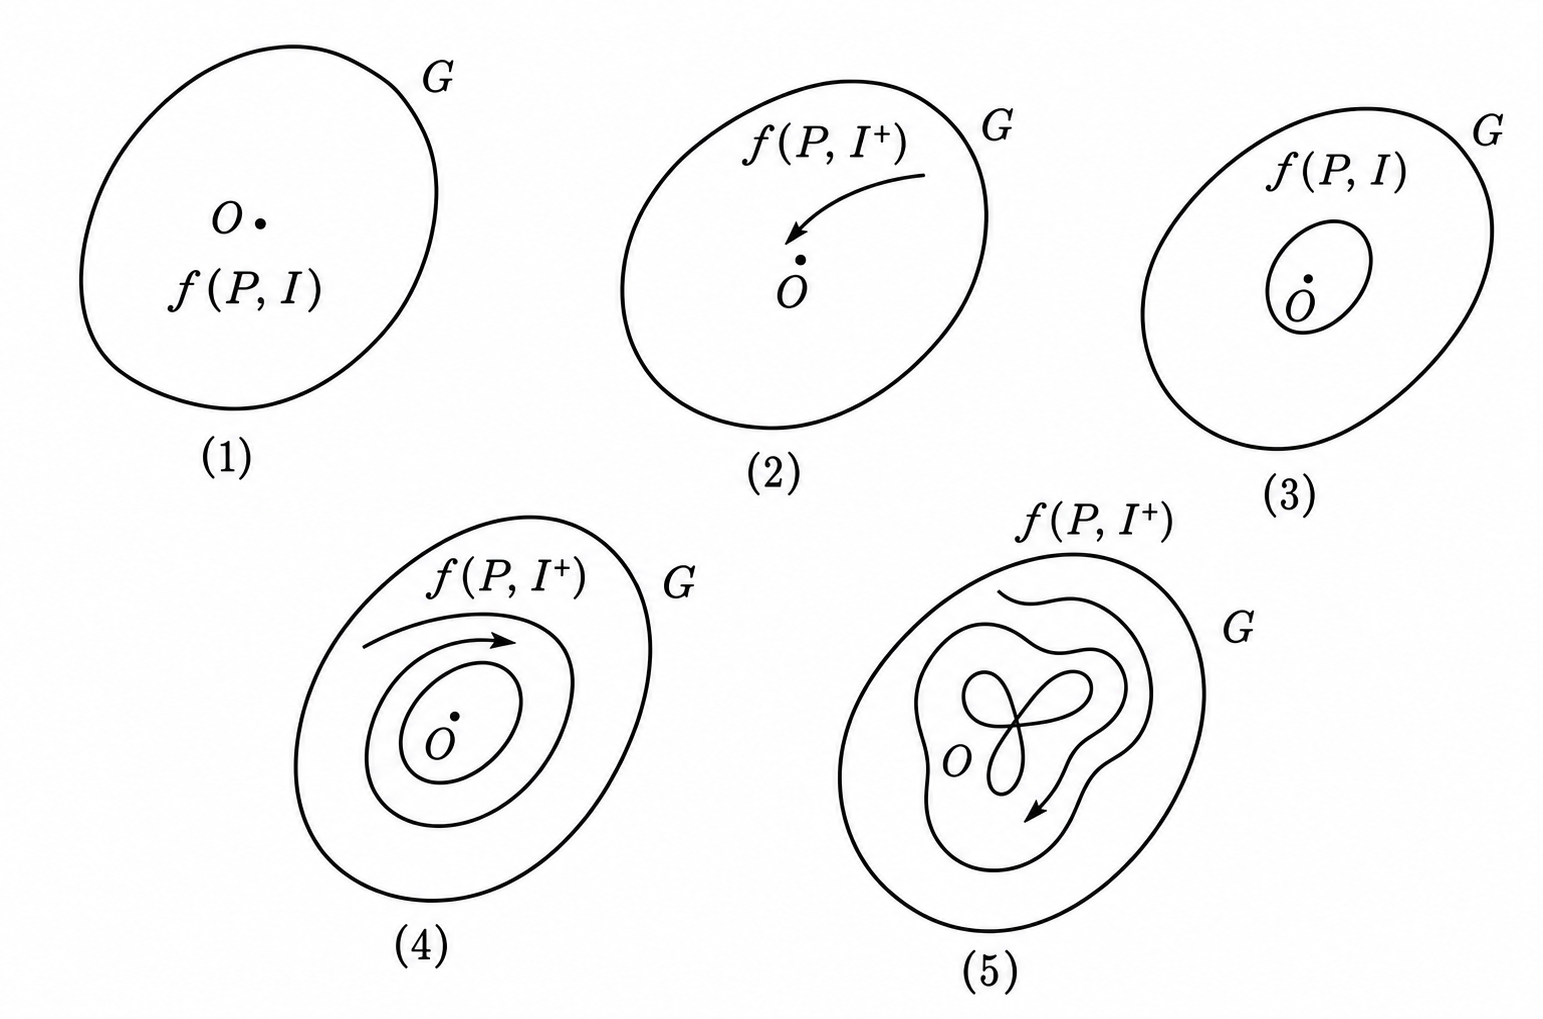
\includegraphics[width=0.7\linewidth]{figure/1.12}
	\captionof{figure}{}
\end{center}
再讨论 $\Omega_P$ 无界的情形.

$S^2$ 是二维球面. $x^*, y^* \in S^2$，定义 $\rho(x^*, y^*)$ 为联接 $x^*$ 和 $y^*$ 的最短球面曲线的长度，于是 $S^2$ 是度量空间. $N$ 是 Euclid 平面的无穷远点. $x^2 + y^2 > r > 0$ 叫做 $N$ 的邻域. $\bar R^2 = \R^2 \cup N$ 叫做将 Euclid 平面封闭化，$\bar R^2$ 是紧致度量空间. 如图所示，$T$ 是测地投影.

\begin{center}
	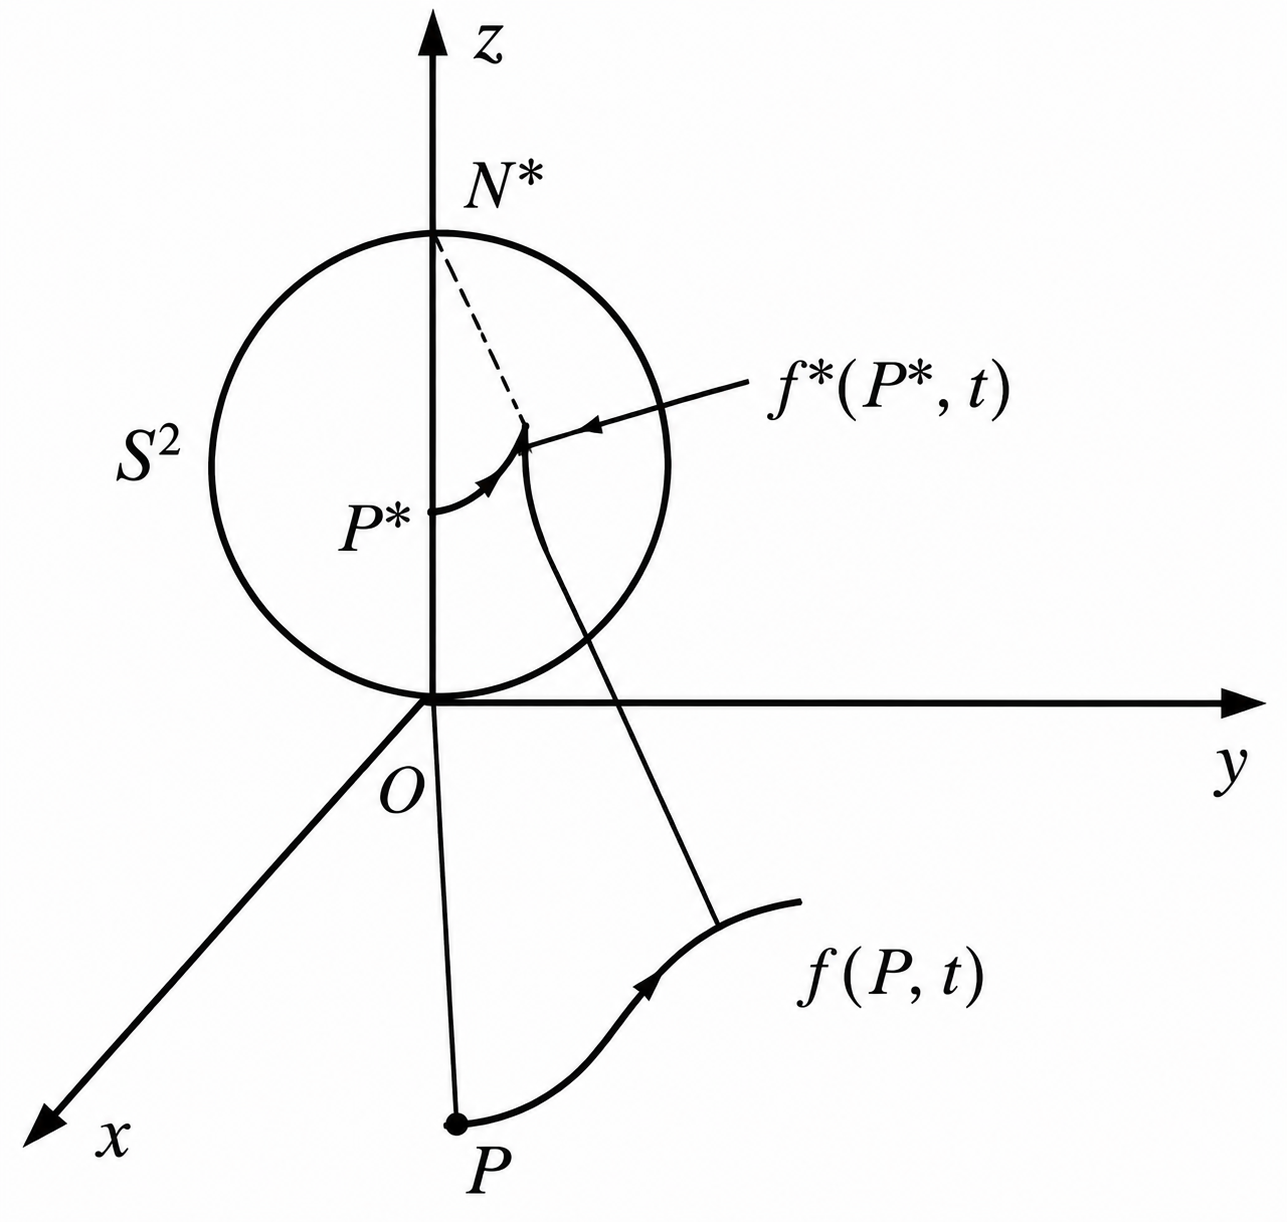
\includegraphics[width=0.5\linewidth]{figure/1.13}
	\captionof{figure}{}
\end{center}

$T: \bar R^2 \to T(\bar R^2) = S^2, N \to T(N) = N^*$. 若 $P \to T(P) = P^*$，定义
\[
f(P, t) \to T(f(P, t)) = f^*(P, t) = \tilde f(P^*, t).
\]
因 $T$ 是拓扑映射，故 $\tilde f(P^*, t)$ 是 $f$ 经过 $T$ 在 $S^2$ 上诱导的动力系统. $\tilde f(N^*, t) = N^*$ 是奇点.

如果 $P_n \to P$，则 $P_n^* \to P^* \neq N^*$；如果 $P_n \to +\infty$，则 $P_n^* \to N^*$. 故若 $\Omega_P$ 有界，则 $\Omega_{P^*} = T(\Omega_P)$；若 $\Omega_P$ 无界，则 $\Omega_{P^*} = T(\Omega_P) \cup N^*$.

\begin{theorem}{}{s2-connected}
$\Omega_{P^*}(A_{P^*})$ 必在 $S^2$ 上连通.
\end{theorem}

\begin{proof}
只证括号外的. 若 $\Omega_P$ 有界，由定理~\ref{thm:omega-connected}, $\Omega_P$ 连通，故 $\Omega_{P^*} = T(\Omega_P)$ 连通. 若 $\Omega_P$ 无界，$\Omega_P \cup N$ 是 $\R^2$ 上的闭集，故 $\Omega_{P^*} = T(\Omega_P) \cup N^*$ 是 $S^2$ 上的闭集. 完全类似定理~\ref{thm:omega-connected} 可证 $S^2$ 上的有界闭集 $\Omega_{P^*}$ 在 $S^2$ 上连通.
\end{proof}

\begin{theorem}{}{unbounded-countable}
如 $\Omega_P$ 无界，$\Omega_P$ 中不包含奇点，则 $\Omega_P$ 至多有可列条无界的轨线组成，而且任何有界区域 $D$ 至多与有限条轨线相交.
\end{theorem}

\begin{proof}
$\Omega_P$ 无界，不包含奇点，故 $\Omega_{P^*} = T(\Omega_P) \cup N^*$, $N^*$ 是 $\Omega_{P^*}$ 中唯一奇点. 类似于定理~\ref{thm:countable} 的推论~1, $\Omega_{P^*}$ 中至多有可列条轨线，每条轨线的正向和负向都接触 $N^*$. 故 $\Omega_P$ 中至多有可列条轨线. 令 $K: x^2 + y^2 \leq r^2$，取 $r$ 充分大，使得 $D \subset K$. 由本节习题 17, $T(\partial K)$ 至多能与 $\Omega_{P^*}$ 中有限条轨线相交，故 $K$ 至多能与 $\Omega_P$ 中有限条轨线相交，故 $D$ 也至多能与 $\Omega_P$ 中有限条轨线相交.
\end{proof}

平面 $\R^2$ 上的区域（连通开集）$D$ 叫做单连通区域，如 $D$ 内任何一条单闭曲线，其内部也属于 $D$.

在平面 $\bar R^2 = \R^2 \cup N$ 上，单连通区域的概念略有不同. $D$ 叫做 $\bar R^2$ 上的单连通区域，如果 $D$ 内任何一条单闭曲线 $l$，或其内部或其外部属于 $D$. 例如平面去掉一点 $P$, $\bar R^2 \setminus \{P\}$ 是 $\bar R^2$ 上的单连通区域，但 $R^2 \setminus \{P\}$ 不是 $R^2$ 上的单连通区域.

$S^2$ 上去掉一点，它是 $S^2$ 上的单连通区域.

在证明下面的定理~\ref{thm:omega-s2-boundary} 之前，我们先举两个例子，来说明单连通区域的边界是连通闭集，它可能是非常复杂的.

\begin{example}{}{sc-region1}
$OBCD$ 是边长为 1 的正方形，正方形内部记成 $K$.
\[
\left.
\begin{aligned}
M_{2k+1}N_{2k+1} &: x = \frac{1}{2^{2k+1}}, \quad 0 \leq y \leq \frac{2}{3}, \\
M_{2(k+1)}M_{2(k+1)} &: x = \frac{1}{2^{2(k+1)}}, \quad \frac{1}{3} \leq y \leq 1,
\end{aligned}
\right\} k = 0, 1, 2, \cdots.
\]
令
\[
G = K \setminus \bigcup_{j=1}^\infty M_jN_j,
\]
$G$ 是单连通区域. 它的边界是
\[
\partial G = \partial K \cup \left(\bigcup_{j=1}^\infty M_jN_j\right).
\]

边界上的点分两类. 一类叫可近边界点，一类叫不可近边界点. $P \in \partial G$ 叫可近边界点，如果存在简单弧段（连续无重点的曲线段）$l \subset G$, $P$ 是 $l$ 的一个端点. $P \in \partial G$ 叫不可近边界点，如果不存在这样的简单弧段. 可近边界点在 $\partial G$ 上处处稠密. 见图~1.14.

在这个例子中，$OD$ 上的点是不可近边界点，其余的边界上的点都是可近边界点. 显然，$\partial G \setminus OD$ 在 $\partial G$ 上处处稠密.
\end{example}
\begin{center}
	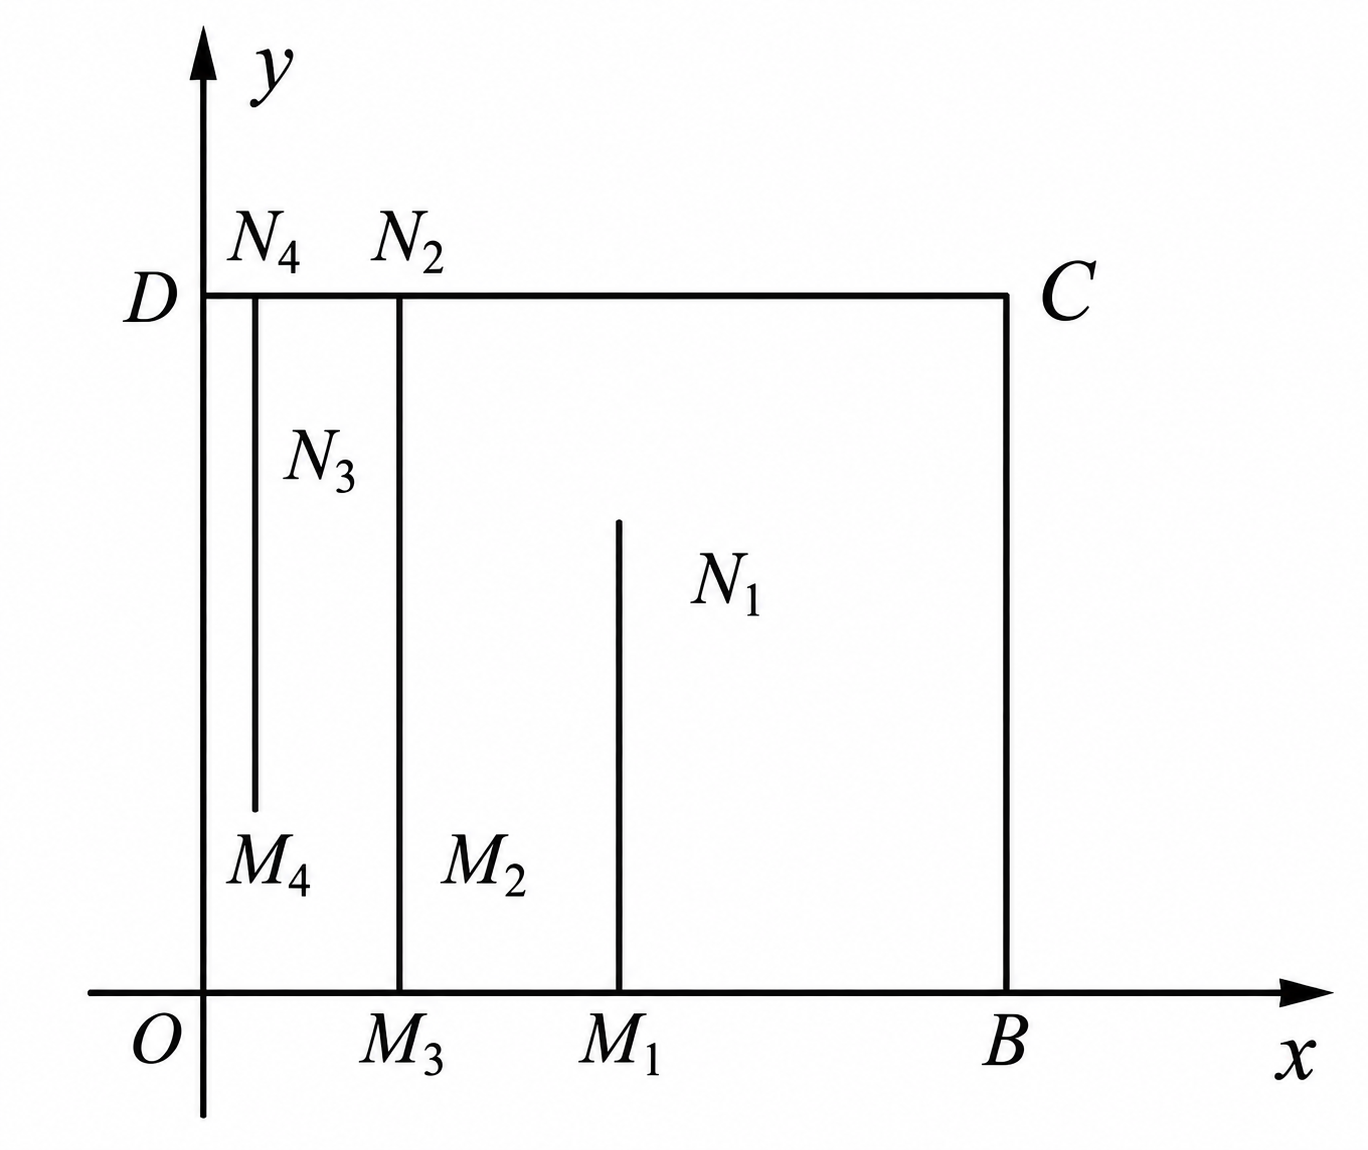
\includegraphics[width=0.4\linewidth]{figure/1.14}
	\captionof{figure}{}
\end{center}


\begin{example}{}{sc-region2}
$K$ 是单位圆的内部. $K$ 内有两个单连通区域 $G_1$ 和 $G_2$，形状都像螺旋线. $G_1$ 是打上阴影的；$G_2$ 是没打阴影的. $G_1$ 和 $G_2$ 有公共的边界.
\[
\partial G_1 = \partial G_2 = L \cup \partial K,
\]
其中 $L$ 是 $G_1$ 和 $G_2$ 的分界.

显然 $L$ 上的点是可近边界点，$\partial K$ 上的点是不可近边界点. $L$ 在 $L \cup \partial K$ 上处处稠密. 见图~1.15.

上例中是两个单连通区域有公共的边界，也可发生更多的单连通区域有公共的边界，这时边界的构造将更加复杂. 请读者参看文献~\cite{aleksandrov-1948} 中的一个有趣的例子.
\end{example}
\begin{center}
	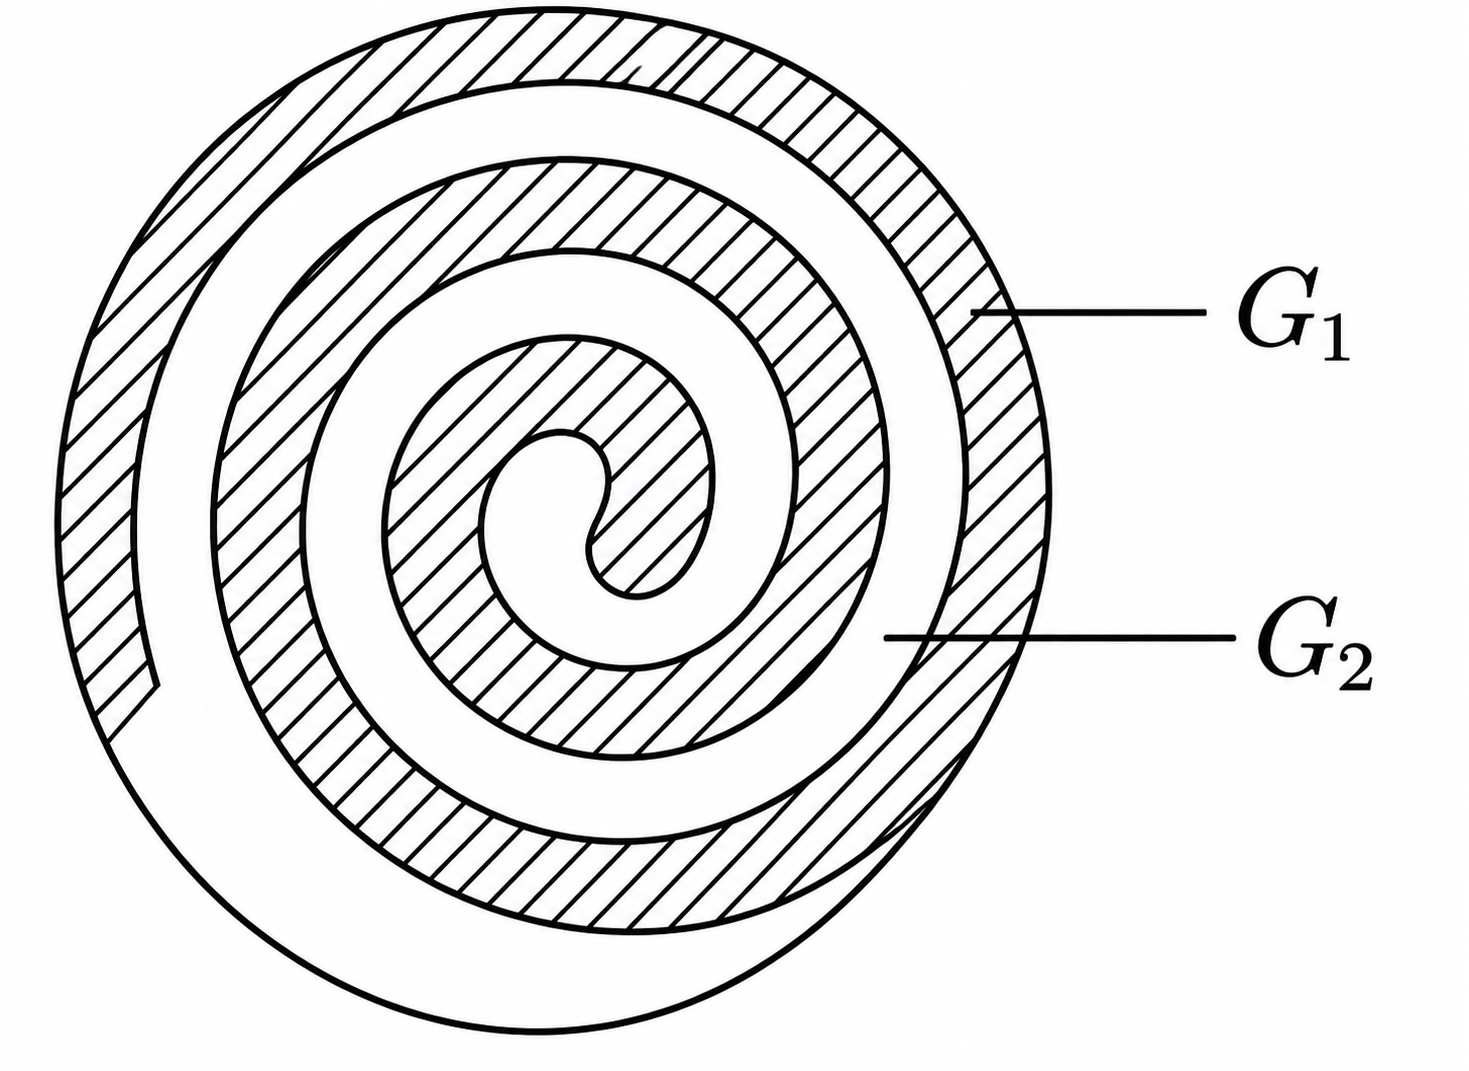
\includegraphics[width=0.4\linewidth]{figure/1.15}
	\captionof{figure}{}
\end{center}

\begin{theorem}{}{omega-s2-boundary}
平面上点集 $E$ 是微分方程所定义的动力系统某一条轨线 $f(P, I)$ 的 $\omega$（或 $\alpha$）极限点集，即 $\Omega_P = E$（或 $A_P = E$），其充要条件为：$T(E) = E^*$ 是 $S^2$ 上单连通区域的边界.
\end{theorem}

\begin{proof}
只证明括号外的情形. 先证必要性.

如果 $\Omega_P \cap f(P, I^+) \neq \emptyset$，则由定理~\ref{thm:poincare}, $E = \Omega_P$ 是奇点或闭轨线，显然 $E^*$ 是 $S^2$ 上单连通区域的边界.

如果 $\Omega_P \cap f(P, I^+) = \emptyset$，则 $\Omega_{P^*} \cap \tilde f(P^*, I^+) = \emptyset$（可能 $N^* \in \Omega_{P^*}$，但 $N^* \notin \tilde f(P^*, I^+)$）. 令 $\Omega_{P^*} = E^*$, $G = S^2 \setminus E^*$. 因 $E^*$ 为闭集，故 $G$ 为开集，$G = \bigcup_\alpha G_\alpha$, $G_\alpha \cap G_\beta = \emptyset$，当 $\alpha \neq \beta$, $G_\alpha$ 为连通分支. 因 $\tilde f(P^*, I^+)$ 连通，$\tilde f(P^*, I) \cap E^* = \emptyset$，故 $\tilde f(P^*, I)$ 必属于其中一个连通分支，设 $\tilde f(P^*, I) \subset G_\alpha$. 于是 $\tilde f(P^*, I)$ 的极限点集 $E^* \subset \bar G_\alpha$，但 $E^* \cap G_\alpha \subset E^* \cap G = \emptyset$，故 $E^* \subset \partial G_\alpha$. 另外 $\partial G_\alpha \subset \partial G = E^*$，故 $E^* = \partial G_\alpha$. 因 $E^*$ 连通，故 $G_\alpha$ 单连通，故 $E^*$ 是单连通区域 $G_\alpha$ 的边界.

现证充分性. 设 $E$ 中只包含一个点，则它为奇点，这时结论自然成立.

设 $E$ 中不只包含一个点，$T(E) = E^*$ 是 $S^2$ 上单连通区域 $G$ 的边界，则 $T^{-1}(G) - D$ 是 $\bar R^2$ 上的单连通区域，$\partial D - E$ 或 $E \cup N$.

可将 $\bar R^2$ 看成完全复平面，即复平面加无穷远点. 令 $K$ 是 $\R^2$ 上以原点为中心的单位圆的内部. 在 $\bar K$ 上考虑微分方程：
\[
\frac{\dd \rho}{\dd t} = \rho(1 - \rho), \quad \frac{\dd \varphi}{\dd t} = 1, \tag{4.2}\label{eq:4.2}
\]
$\rho = 0$ 是奇点，$\rho = 1$ 是闭轨线. 对任何点 $P \in K$，当 $P$ 不是奇点，有 $\Omega_P = \partial K, A_P = \{O\}$. (4.2) 的任一解都在整个实轴上定义.

由 Riemann 映射定理~\cite{ahlfors-1966}，对 $R^2$ 上任何边界多于一个点的单连通区域 $D$ 必存在一个解析函数
\[
w = f(z) = u(x, y) + iv(x, y),
\]
双方单值保角地将单位圆 $K$ 的内部映射到 $D$ 上. 于是
\[
F: u = u(x, y); v = v(x, y)
\]
是拓扑映射，将 $K$ 变到 $D$，并且
\[
\frac{\partial(u, v)}{\partial(x, y)} \neq 0.
\]

故 $F$ 将方程 \eqref{eq:4.2} 变为
\[
\frac{\dd u}{\dd t} = P(u, v), \quad \frac{\dd v}{\dd t} = Q(u, v). \tag{4.3}\label{eq:4.3}
\]
其解为 $u = u(x(t), y(t)), v = v(x(t), y(t)), -\infty < t < +\infty$，故 \eqref{eq:4.3} 是动力系统.

一般来说，在变换 $F$ 下，边界 $\partial K$ 到边界 $\partial D$ 的对应不见得是一对一的，但由 Riemann 定理，端点在 $E = \partial D$ 上的简单弧段 $S$，其原像 $l$ 也是端点在 $\partial K$ 上的简单弧段，设 $S$ 在 $E$ 上的端点是 $B_2$, $l$ 在 $\partial K$ 上的端点是 $B_1$. 对 \eqref{eq:4.2} 而言，若 $P_1 \in K$，但 $P_1$ 不是奇点，则有 $\Omega_{P_1} = \partial K$. 由定理~\ref{thm:closed-nearby}, \eqref{eq:4.2} 的轨线 $f(P_1, I^+)$ 绕 $\partial K$ 盘旋. 设 $f(P_1, I^+) \cap l = f(P_1, t_n) = \{M_n\}$, $M_n \to B_1$，当 $t_n \to +\infty$. 设 $F(P_1) = P_2$，因 $F$ 是保角映射，则对 \eqref{eq:4.3} 的轨线 $f(P_2, I^+)$，有 $f(P_2, I^+) \cap S = f(P_2, \tilde t_n) = \{N_n\}$, $N_n \to B_2$，当 $\tilde t_n \to +\infty$. 故 $B_2 \in \Omega_{P_2}$. 这样 $E$ 上的可近边界点都属于 $\Omega_{P_2}$. 但 $E$ 上的可近边界点在 $E$ 上处处稠密，因 $\Omega_{P_2}$ 是闭集，故 $E \subset \Omega_{P_2}$. 另外 $\Omega_{P_2}$ 中不可能有 $E$ 之外的点，否则 $\Omega_{P_2}$ 中将有 $\partial K$ 之外的点. 故 $E = \Omega_{P_2}$.
\end{proof}

由例题~\ref{ex:sc-region1}, \ref{ex:sc-region2} 可见，在平面 $\R^2$ 上，轨线 $L_P$ 的 $\omega$ 或 $\alpha$ 极限集 $\Omega_P$ 或 $A_P$ 的构造已可能是很复杂的了. 而在 $R^n (n \geq 3)$ 中极限集 $\Omega_P$ 或 $A_P$ 的构造更可能是异常复杂的.

当 $\Omega_P$ 无界时，经过测地投影，$\Omega_{P^*} \to \Omega_{P^*} \in S^2$，因 $\Omega_{P^*}$ 中包含 $N^*$，故 $\Omega_{P^*}$ 是 $S^2$ 上的有界闭集，故 $\Omega_{P^*}$ 是 $S^2$ 上的有界连通集. 这时凡是平面上关于 $\Omega_P$ 有界时的结论都可以相应地搬到 $\Omega_{P^*}$ 上来，然后再返回 $R^2$ 上，这就是为什么要到 $S^2$ 上去研究问题的理由.

% ============================================================
%  习题和参考文献
% ============================================================
\section*{习题}

\begin{enumerate}
\item 设数值函数 $a(t)$ 在 $0<t<t_1$ 上连续且
\[
	\int_{0+}^{t_1} a(t)\,\dd t
\]
收敛，求证方程
\[
	\dfrac{\dd x}{\dd t}=a(t)x
\]
的满足条件 $\lim\limits_{t\to0+}x(t)=0$ 的解只有一个。

\item 设 $f(x)$ 在 $x\in\R$ 上连续，证明
\[
	\dfrac{\dd x}{\dd t}=f^2(x)+\mathrm{e}^{-t}
\]
具有解的唯一性。

\item 设函数 $f(t,x)$ 与 $F(t,x)$ 在区域 $G$ 上连续，满足 Lipschitz 条件，且到处都有
\[
	f(t,x)\leq F(t,x).
\]
设 $x=\varphi(t)$ 与 $x=\Phi(t)$ 分别是方程
\[
	\dfrac{\dd x}{\dd t}=f(t,x)
	\quad\text{与}\quad
	\dfrac{\dd x}{\dd t}=F(t,x)
\]
的满足同一初值条件 $x(t_0)=x_0$ 的解，它们的共同存在区间是 $a\leq t\leq b$，则
\[
	\varphi(t)\leq\Phi(t)\quad\text{当}\quad t_0\leq t\leq b,
\]
\[
	\varphi(t)\geq\Phi(t)\quad\text{当}\quad a\leq t\leq t_0.
\]
提示：\quad(i) 当 $f(t,x)<F(t,x)$ 时，结论成立。\\
\phantom{提示：}\quad(ii) 考虑方程
\[
	\begin{cases}
		\dfrac{\dd x}{\dd t}=f(t,x)+\varepsilon_m,\\
		x(t_0)=x_0,
	\end{cases}
\]
的解，$\varepsilon_m>0$ 且当 $m\to\infty$ 时单调地趋于零。

\item 讨论方程
\[
	\dfrac{\dd x}{\dd t}=(2-x-x^2)\mathrm{e}^{(t-1)x^2}
\]
的每一积分曲线的两端的性状，并画出积分曲线族的大概图形。\\
提示：\quad(i) 当 $t_0\leq1$ 时，每一积分曲线的左侧都有水平渐近线。\\
\phantom{提示：}\quad(ii) 每一条水平直线，都有一积分曲线的左侧以它为渐近线。\\
\phantom{提示：}\quad(iii) 在 $t>1$ 半平面上，每一条垂直于 $x$ 轴的直线都有二条积分曲线分别以它为垂直渐近线。

\item 若 $f(t,x)$ 在 $G$ 上连续，且满足条件
\[
	\|f(t,x_1)-f(t,x_2)\|\leq L(\|x_1-x_2\|),
\]
当 $(t,x_1),(t,x_2)\in G$，其中 $L(r)$ 在 $0\leq r<r_0$ 上连续，$L(r)>0$，且
\[
	\int_0^{r_0}\dfrac{\dd r}{L(r)}=+\infty,
\]
则 Cauchy 问题
\[
	\begin{cases}
		\dfrac{\dd x}{\dd t}=f(t,x),\\
		x(t_0)=x_0
	\end{cases}
\]
的解 $x=x(t,t_0,x_0)$ 对初值是连续的。

\item 设 $f_k(x,y_1,\cdots,y_n)$ 在区域
\[
	D\bigl(|x-x_0|\leq a,\ |y_1|<+\infty,\ \cdots,\ |y_n|<+\infty\bigr)
\]
上连续，且对 $y_1,\cdots,y_n$ 有连续的偏微商。又设在 $D$ 上 $f_k$ 满足不等式
\[
	|f_k|\leq L\sum_{i=1}^n|y_i|+M\qquad(i=1,2,\cdots,n).
\]
其中 $L$ 与 $M$ 是正常数，则相应的 Cauchy 问题
\[
	\dfrac{\dd y_k}{\dd x}=f_k(x,y_1,\cdots,y_n)qquad(i=1,2,\cdots,n),
\]
\[
	y_k(x_0)=y_k^0
\]
在区间 $|x-x_0|\leq a$ 上恰有一解。

\item 设微分方程 $(D)$：
\[
	\dfrac{\dd y}{\dd x}=\lambda(1+\sin^2x+\sin^2y)+x,
\]
其中 $\lambda$ 是参数。又设边界条件 $(E)$：
\[
	y(0)=0,\qquad y(1)=0.
\]
试证，存在 $\lambda=\lambda_0$，问题 $(D)+(E)$ 有解。

\item 设给定方程
\[
	\dfrac{\dd x}{\dd t}=\sin(tx),
\]
试求
\[
	\left[\dfrac{\partial x}{\partial t_0}(t,t_0,x_0)\right]_{\substack{t_0=0\\x_0=0}},
	\qquad
	\left[\dfrac{\partial x}{\partial x_0}(t,t_0,x_0)\right]_{\substack{t_0=0\\x_0=0}}.
\]

\item 设 $f_i(t,\vect{x})$ 连续可微 $(i=1,2,\cdots,n)$，则 Cauchy 问题
\[
	\dfrac{\dd x_i}{\dd t}=f_i(t,\vect{x}),\qquad
	\vect{x}(t_0)=\vect{x}_0\qquad(i=1,2,\cdots,n)
\]
的解 $\vect{x}=\varphi(t,t_0,\vect{x}_0)$ 满足恒等式
\[
	\dfrac{\partial\varphi(t,t_0,\vect{x}_0)}{\partial t_0}
	+\sum_{i=1}^n\dfrac{\partial\varphi(t,t_0,\vect{x}_0)}{\partial x_i^0}
	f_i(t_0,\vect{x}_0)\equiv0.
\]

\item 设 Cauchy 问题
\[
	\begin{cases}
		\dfrac{\dd y}{\dd x}=f(x,y,\mu),\\
		y(x_0)=y_0
	\end{cases}
\]
的解为 $y^*=y^*(x;x_0,y_0,\mu)$。试证，若
\[
	\left(\dfrac{\partial y^*}{\partial x_0}\right)
	\quad\text{与}\quad
	\left(\dfrac{\partial y^*}{\partial\mu}\right)
\]
存在，则
\[
	\left(\dfrac{\partial y^*}{\partial x_0}\right)_{x=x_0}
	=-f(x_0,y_0;\mu),\qquad
	\left(\dfrac{\partial y^*}{\partial\mu}\right)_{x=x_0}=0.
\]

\item 试证在上题中有公式
\[
	\dfrac{\partial y^*}{\partial x_0}
	=-f(x_0,y_0;\mu)
	\exp\!\left\{\int_{x_0}^x f_y'(x,y^*;\mu)\,\dd x\right\}
\]
与
\[
	\dfrac{\partial y^*}{\partial\mu}
	=\exp\!\left\{\int_{x_0}^x f_y'(x,y^*;\mu)\,\dd x\right\}
	\cdot\int_{x_0}^x f_\mu'(x,y^*,\mu)
	\exp\!\left\{-\int_{x_0}^x f_y'(x,y^*;\mu)\,\dd x\right\}\,\dd x.
\]
并同时写出 $\dfrac{\partial y^*}{\partial x_0}$ 与 $\dfrac{\partial y^*}{\partial\mu}$ 所满足的微分方程。

\item 设 $f(t,x,y)$ 在区域 $G(0\leq t\leq1,-\infty<x<+\infty,-\infty<y<+\infty)$ 上有连续的偏微商，$\varphi(t)$ 是边值问题
\[
	\begin{cases}
		x''=f(t,x,x'),\\
		x(0)=a,\qquad x(1)=b
	\end{cases}
\]
的解。又设在区域 $G$ 上 $\dfrac{\partial f}{\partial x}>0$，试证，对充分靠近 $b$ 的 $\beta$，边值问题
\[
	\begin{cases}
		x''=f(t,x,x'),\\
		x(0)=a,\qquad x(1)=\beta
	\end{cases}
\]
有解。\\
提示：设满足条件 $\theta(0,\alpha)=a$，$\theta'(0,\alpha)=\alpha$ 的解为 $\theta(t,\alpha)$。令 $\varphi'(0)=\alpha_0$，于是当 $|\alpha-\alpha_0|$ 充分小时，$\theta$ 在区间 $t\in[0,1]$ 上存在。设
\[
	u(t)=\dfrac{\partial\theta(t,\alpha_0)}{\partial\alpha},
\]
于是
\[
	u''-\dfrac{\partial f}{\partial y}\bigl(t,\varphi(t),\varphi'(t)\bigr)u'
	-\dfrac{\partial f}{\partial x}\bigl(t,\varphi(t),\varphi'(t)\bigr)u=0,
\]
其中 $u(0)=0$，$u'(0)=1$。因为 $\dfrac{\partial f}{\partial x}>0$，所以 $u$ 是单调上升和 $u(1)=\dfrac{\partial\theta}{\partial\alpha}(1,\alpha_0)>0$。这样方程
\[
	\theta(1,\alpha)-\beta=0
\]
在 $(\alpha_0,b)$ 的充分小邻域可解出 $\alpha$ 是 $\beta$ 的函数。

\item 试证明，设 $f(x)$ 在定义区域上对 $x$ 连续，则 Cauchy 问题 (2.3)、(2.4) 的解对初值的连续依赖性与解的唯一性等价。

\item 定理 3.4 中的有界性条件是否可缺少？试举例说明。

\item 如 $f(P,I^+)$ 有界，能否证明 $\Omega_P$ 是曲线连通？

\item 试证明，任何轨线 $f(P,I)$ 在 $\R^2$ 上无处稠密。

\item 试证明，在定理 4.10 的推论 1 中，任何以 $O$ 为圆心的圆周只能与 $\Omega_P^{(1)}$ 中的有限条轨线相交。

\item 试证明，设 $\Omega_P$ 有界，$\Omega_P$ 非闭轨线，则对任何 $R\in\Omega_P$，$\Omega_R$ 和 $A_R$ 必为奇点。

\item 试证明，设 $\Omega_P$ 无界，$\Omega_P$ 中无奇点，则 $\Omega_P$ 中无有界分支。

\item 试举例说明，当 $\Omega_P$ 无界，$\Omega_P$ 中有奇点，则 $\Omega_P$ 中可以有有界分支，而且有界分支必通过奇点与 $\Omega_P$ 中的无界分支相联接。

\item 试由动力系统的性质 II，推证在任何有限时间区间上，解对初值连续依赖。
\end{enumerate}

\section*{参考文献}

\begin{enumerate}
\item Немыцкий，В. В. и Степанов，В. В.，\textit{Качественная теория дифференциальных уравнений}，М.，Л.，Гостехиздат，1949（中译本：В. В. 涅梅茨基、В. В. 斯捷巴诺夫，\textit{微分方程定性理论}，上、下册，科学出版社，1956，1959。）
\item 秦元勋，\textit{微分方程所定义的积分曲线}，上、下册，科学出版社，1959。
\item 叶彦谦，\textit{极限环论}，上海科学技术出版社，1965。
\item Coddington, E. A. and Levinson, N., \textit{Theory of ordinary differential equations}, McGraw-Hill, New York, 1955.
\item Александров，П. С.，\textit{Введение в общую теорию множеств и функций}，Гостехиздат，1948。
\item Ahlfors, L., \textit{Complex Analysis}, McGraw-Hill, New York, 1966.
\end{enumerate}



%
%% 第二章  平面奇点
%% ============================================================
%  chapter02.tex — 第二章 平面奇点
%  对应原书第二章。
%  研究平面自治系统平衡点的分类与判定：线性近似、非线性扰动、
%  中心—焦点判别、几何分类及零特征根情形。
% ============================================================

\setchapterimage{}
\setchapterintro{}
\chapter{平面奇点}

\newcommand{\chTwoFigurePlaceholder}[1]{%
  \begin{center}
    \fbox{\parbox{0.72\textwidth}{\centering\vspace{2.7cm}图~#1\\（图片占位）\vspace{2.7cm}}}
  \end{center}%
}

% ============================================================
%  §1  奇点和常点
% ============================================================
\section{奇点和常点}

给定微分方程组
\[
\left\{
\begin{aligned}
\dfrac{dx}{dt}&=X(x,y),\\
\dfrac{dy}{dt}&=Y(x,y),
\end{aligned}
\right.\tag{1.1}
\]
其中 $X(x,y),Y(x,y)\in C^0(D)$，$D\subseteq\mathbb{R}^2$。方程组(1.1)在奇点及常点有完全不同的性质。

从解析的观点看，若 $P_0(x_0,y_0)\in D$ 满足
\[
X^2(x_0,y_0)+Y^2(x_0,y_0)=0,
\]
则称 $P_0$ 为方程组(1.1)的一个奇点。这时 $x=x_0,y=y_0$ 是方程组(1.1)的一个解。若
\[
X^2(x_0,y_0)+Y^2(x_0,y_0)\ne0,
\]
则称 $P_0$ 为方程组(1.1)的一个常点。从拓扑的观点看，奇点是方程组(1.1)所定义的向量场在 $P_0$ 点的向量 $(X,Y)$ 为零的点；常点则是该向量不为零的点。从力学的观点看，若 $x$ 表示位置，则 $dx/dt$ 表示速度，$dy/dt=d^2x/dt^2$ 表示加速度；奇点是平衡位置，常点不是平衡位置。

\subsection*{常点附近轨线的拓扑结构}

在常点 $P_0$ 的邻域内，经一个非退化的线性坐标变换，可把 $P_0$ 移至原点，并使向量场在原点的方向为 $y$ 轴的方向。为简单起见，设方程组(1.1)满足
\[
x_0=y_0=0,\qquad X(0,0)=0,\qquad Y(0,0)\ne0.
\]
在充分小的圆邻域 $S(O,\varepsilon)$ 内 $Y(x,y)\ne0$，方程组(1.1)等价于
\[
\dfrac{dx}{dy}=\dfrac{X(x,y)}{Y(x,y)}.\tag{1.2}
\]
它的解可写成 $x=x(y,a)$，其中 $x(0,a)=a$。

\begin{center}
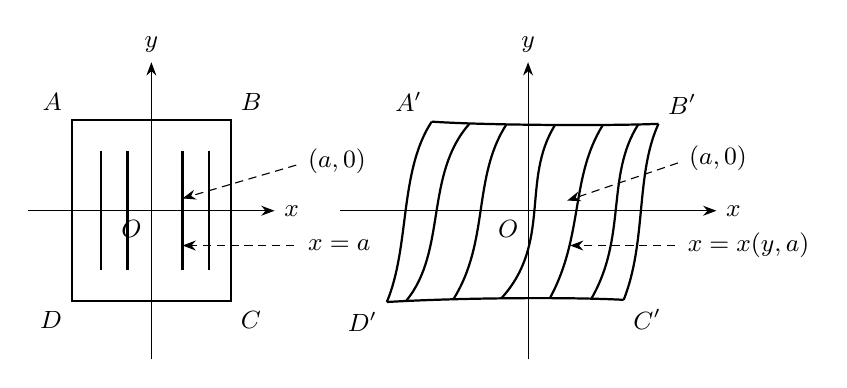
\begin{tikzpicture}[x=0.92cm,y=0.92cm,>=Stealth,font=\small]
  % 左图：参数直线族所在的长方形
  \draw[->] (-3.75,0) -- (-0.35,0) node[right] {$x$};
  \draw[->] (-2.05,-2.05) -- (-2.05,2.05) node[above] {$y$};
  \node[below left] at (-2.05,0) {$O$};
  \draw[thick] (-3.15,1.25) rectangle (-0.95,-1.25);
  \node[above left] at (-3.15,1.25) {$A$};
  \node[above right] at (-0.95,1.25) {$B$};
  \node[below right] at (-0.95,-1.25) {$C$};
  \node[below left] at (-3.15,-1.25) {$D$};
  \foreach \xx in {-2.75,-2.38,-1.62,-1.25}
    \draw[thick] (\xx,-0.82) -- (\xx,0.82);
  \draw[thick] (-1.62,-0.82) -- (-1.62,0.82);
  \draw[densely dashed,->] (-0.05,0.63) -- (-1.62,0.17);
  \node[anchor=west] at (-0.02,0.68) {$(a,0)$};
  \draw[densely dashed,->] (-0.08,-0.48) -- (-1.62,-0.48);
  \node[anchor=west] at (-0.02,-0.48) {$x=a$};

  % 右图：微分同胚下的曲边四边形及积分曲线族
  \draw[->] (0.55,0) -- (5.75,0) node[right] {$x$};
  \draw[->] (3.15,-2.05) -- (3.15,2.05) node[above] {$y$};
  \node[below left] at (3.15,0) {$O$};
  \draw[thick] (1.82,1.23) .. controls (2.55,1.18) and (4.26,1.17) .. (4.95,1.20);
  \draw[thick] (1.20,-1.26) .. controls (2.20,-1.20) and (3.75,-1.19) .. (4.47,-1.23);
  \draw[thick] (1.20,-1.26) .. controls (1.52,-0.50) and (1.37,0.55) .. (1.82,1.23);
  \draw[thick] (4.47,-1.23) .. controls (4.79,-0.42) and (4.63,0.50) .. (4.95,1.20);
  \draw[thick] (1.47,-1.24) .. controls (2.03,-0.56) and (1.72,0.50) .. (2.34,1.20);
  \draw[thick] (2.12,-1.22) .. controls (2.62,-0.42) and (2.38,0.46) .. (2.85,1.19);
  \draw[thick] (2.78,-1.21) .. controls (3.48,-0.44) and (3.05,0.42) .. (3.52,1.18);
  \draw[thick] (3.45,-1.21) .. controls (3.92,-0.34) and (3.73,0.45) .. (4.18,1.18);
  \draw[thick] (4.02,-1.22) .. controls (4.52,-0.36) and (4.22,0.48) .. (4.67,1.19);
  \node[above left] at (1.82,1.23) {$A'$};
  \node[above right] at (4.95,1.20) {$B'$};
  \node[below right] at (4.47,-1.23) {$C'$};
  \node[below left] at (1.20,-1.26) {$D'$};
  \draw[densely dashed,->] (5.22,0.66) -- (3.69,0.14);
  \node[anchor=west] at (5.24,0.72) {$(a,0)$};
  \draw[densely dashed,->] (5.18,-0.48) -- (3.73,-0.48);
  \node[anchor=west] at (5.22,-0.48) {$x=x(y,a)$};
\end{tikzpicture}
\captionof{figure}{常点邻域内平行直线族与积分曲线族的对应}
\end{center}


变换
\[
T:(a,y)\longmapsto (x(y,a),y)
\]
把矩形 $ABCD$ 一一地变为曲边四边形 $A'B'C'D'$，并把平行直线族 $x=a$ 变为积分曲线族 $x=x(y,a)$。若 $X,Y\in C^r(D)$，$r\ge1$，由第一章\S1可知 $T\in C^r(y,a)$。现证明 $T^{-1}\in C^r$。

由(1.2)，
\[
\dfrac{d(\partial x/\partial a)}{dy}
=\dfrac{Y\dfrac{\partial X}{\partial x}-X\dfrac{\partial Y}{\partial x}}{Y^2}
\dfrac{\partial x}{\partial a}.
\]
故
\[
\dfrac{d}{dy}\left\{\dfrac{\partial x}{\partial a}
\exp\left[-\int_0^y
\dfrac{YX_x-XY_x}{Y^2}\,dy\right]\right\}=0.
\]
又因 $x(0,a)=a$，所以
\[
\dfrac{\partial x}{\partial a}
=\exp\left\{\int_0^y\dfrac{YX_x-XY_x}{Y^2}\,dy\right\}\ne0.
\]
因此存在反变换
\[
T^{-1}:(x,y)\longmapsto (a(x,y),y),\qquad a(x,0)=x,
\]
它把积分曲线变为直线 $x=a$；由反函数定理 $T^{-1}\in C^r(x,y)$。所以，当 $X,Y\in C^r(D)$，$r\ge1$ 时，常点 $P_0$ 的充分小邻域内的积分曲线可经一个 $C^r$ 微分同胚变为一族平行直线。常点附近的拓扑结构是简单的；奇点附近的情形则复杂得多。

% ============================================================
%  §2  常系数线性方程组的奇点
% ============================================================
\section{常系数线性方程组的奇点}

考虑常系数线性方程组
\[
\left\{
\begin{aligned}
\dfrac{dx}{dt}&=ax+by,\\
\dfrac{dy}{dt}&=cx+dy.
\end{aligned}
\right.\tag{2.1}
\]
其中 $a,b,c,d$ 均为实数。其特征方程为
\[
D(\lambda)=\begin{vmatrix}a-\lambda&b\\c&d-\lambda\end{vmatrix}
=\lambda^2-(a+d)\lambda+ad-bc=0.
\]
令 $p=-(a+d)$，$q=ad-bc$，则 $D(\lambda)=\lambda^2+p\lambda+q$，
\[
\lambda_{1,2}=\dfrac{-p\pm\sqrt{p^2-4q}}{2}.
\]
以下讨论原点的九种情形。

\textbf{1.}\ $q<0$。特征根为异号实根。若 $c\ne0$，取
\[
x'=-cx+(a-\lambda_1)y,\qquad y'=-cx+(a-\lambda_2)y;\tag{2.2}
\]
若 $b\ne0$，取
\[
x'=(d-\lambda_1)x-by,\qquad y'=(d-\lambda_2)x-by.\tag{2.3}
\]
方程组化为
\[
\dfrac{dx'}{dt}=\lambda_1x',\qquad
\dfrac{dy'}{dt}=\lambda_2y'.\tag{2.4}
\]
解为 $x'=C_1e^{\lambda_1t}$，$y'=C_2e^{\lambda_2t}$，从而
\[
y'=C_3|x'|^{\lambda_2/\lambda_1},\qquad \lambda_2/\lambda_1<0.
\]
除两坐标轴外，轨线在两个方向均趋于无穷远；原点为鞍点。

\begin{center}
	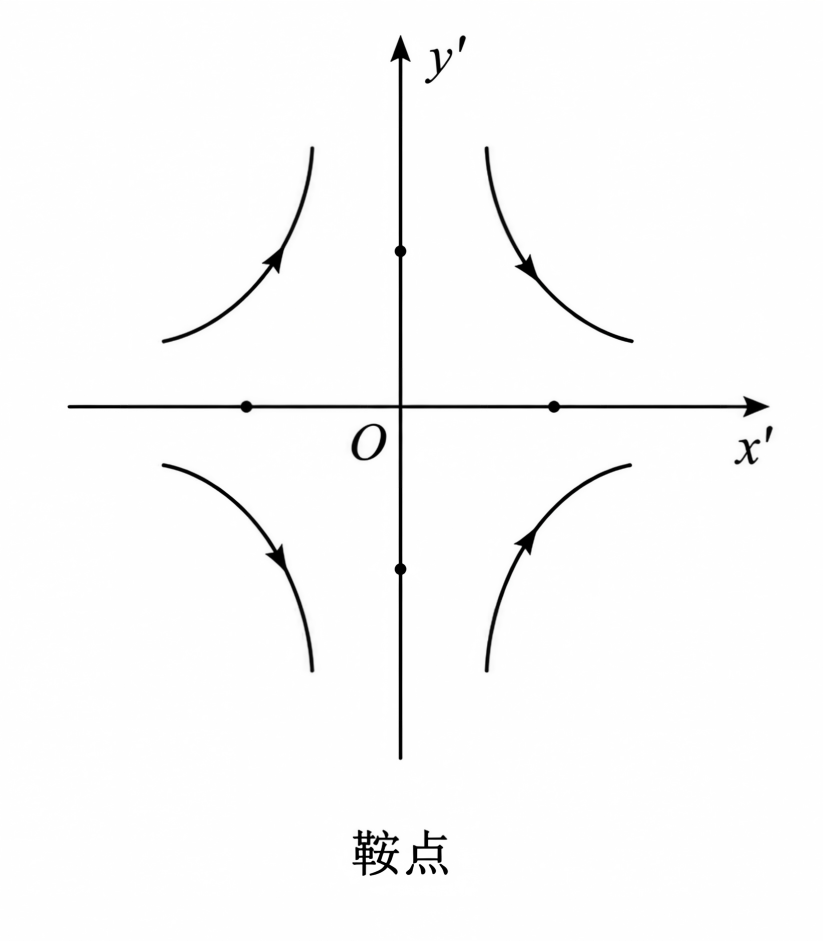
\includegraphics[width=0.4\linewidth]{figure/2.2}
	\captionof{figure}{鞍点}
\end{center}


\textbf{2.}\ $q>0,p>0,p^2-4q>0$。两个特征根均为负实根。由(2.2)或(2.3)化为(2.4)，此时 $\lambda_2/\lambda_1>0$，当 $t\to+\infty$ 时所有轨线均趋于原点。原点为稳定结点。

\begin{center}
	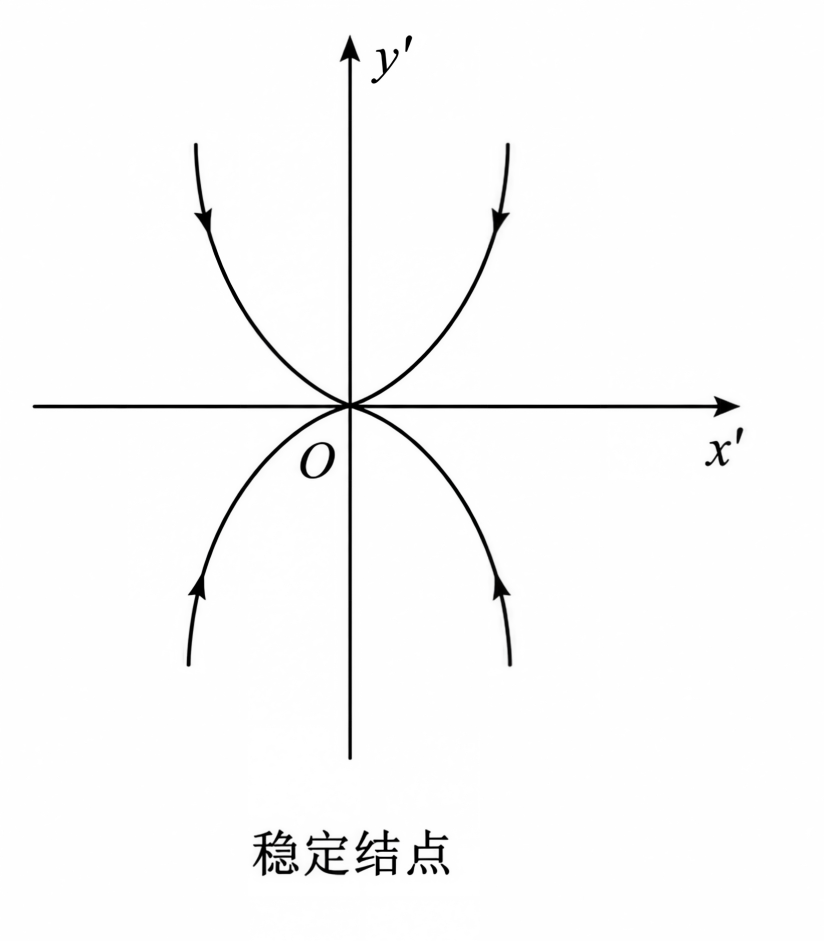
\includegraphics[width=0.4\linewidth]{figure/2.3}
	\captionof{figure}{稳定结点}
\end{center}


\textbf{3.}\ $q>0,p>0,p^2-4q<0$。特征根为
\[
\mu_1\pm i\mu_2,\qquad \mu_1=-\dfrac p2<0,
\]
并可化为
\[
\dfrac{dx'}{dt}=\mu_1x'+\mu_2y',\qquad
\dfrac{dy'}{dt}=-\mu_2x'+\mu_1y'.\tag{2.5}
\]
令 $x'=r\cos\theta,y'=r\sin\theta$，得
\[
\dfrac{dr}{dt}=\mu_1r,\qquad \dfrac{d\theta}{dt}=-\mu_2.\tag{2.6}
\]
故 $r=r(0)e^{\mu_1t}$，$\theta=-\mu_2t+\theta(0)$，所有轨线螺旋形趋于原点；原点为稳定焦点。

\begin{center}
	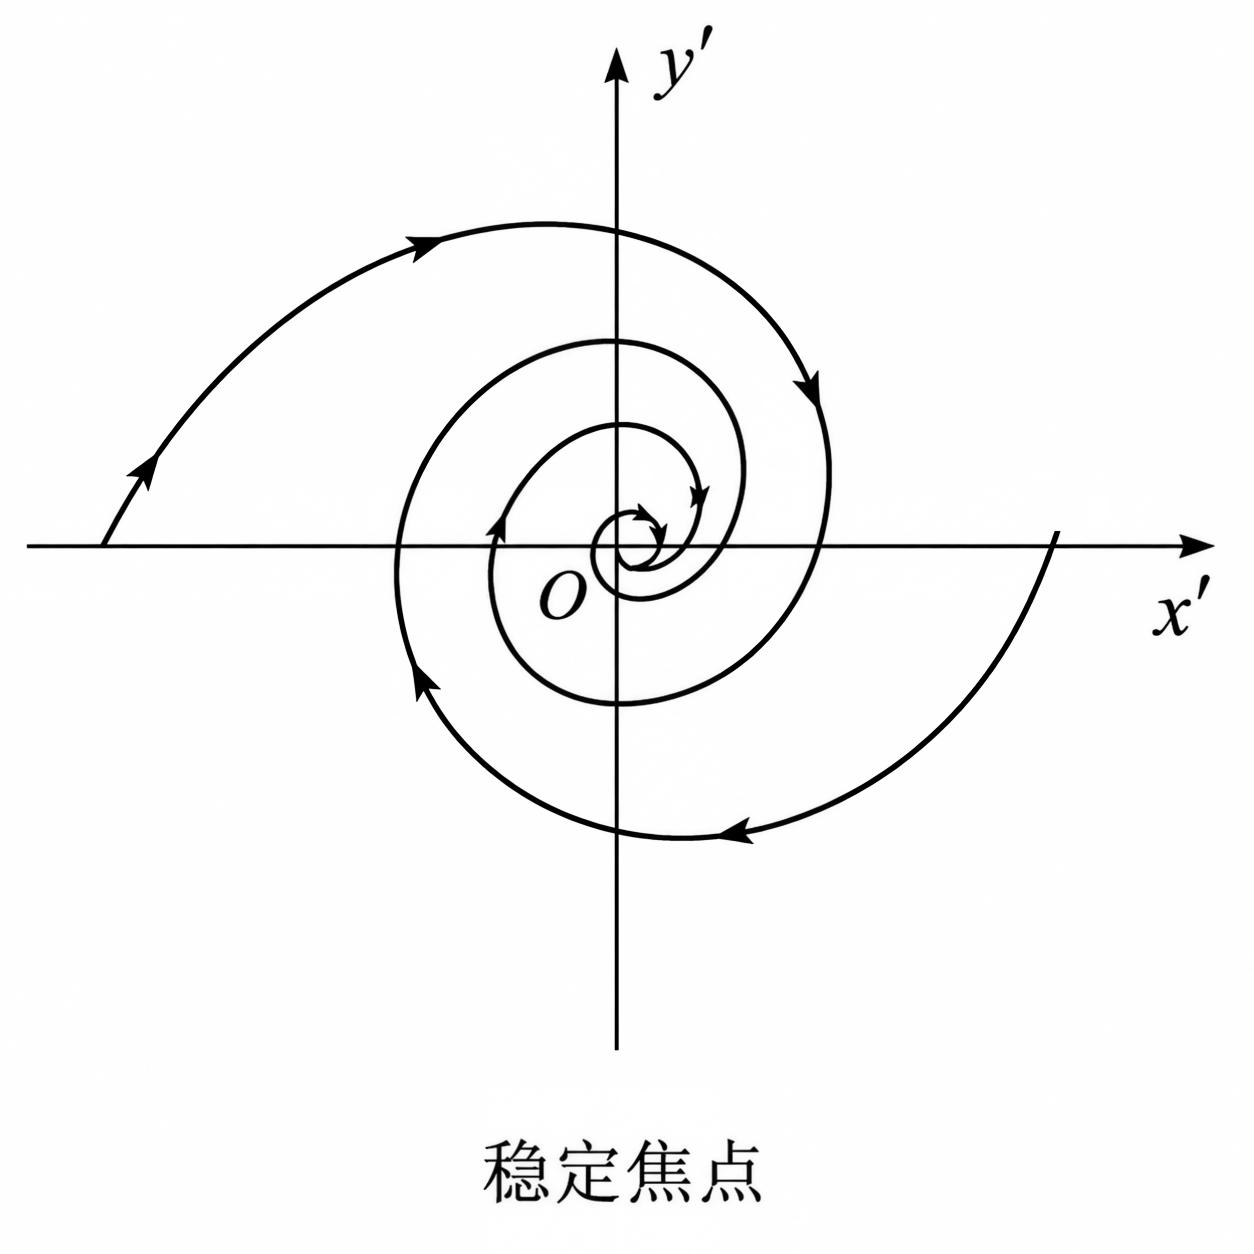
\includegraphics[width=0.4\linewidth]{figure/2.4}
	\captionof{figure}{稳定焦点}
\end{center}

\textbf{4.}\ $q>0,p<0,p^2-4q>0$。经时间反向，得到两个正实根的情形；原点为不稳定结点。

\begin{center}
	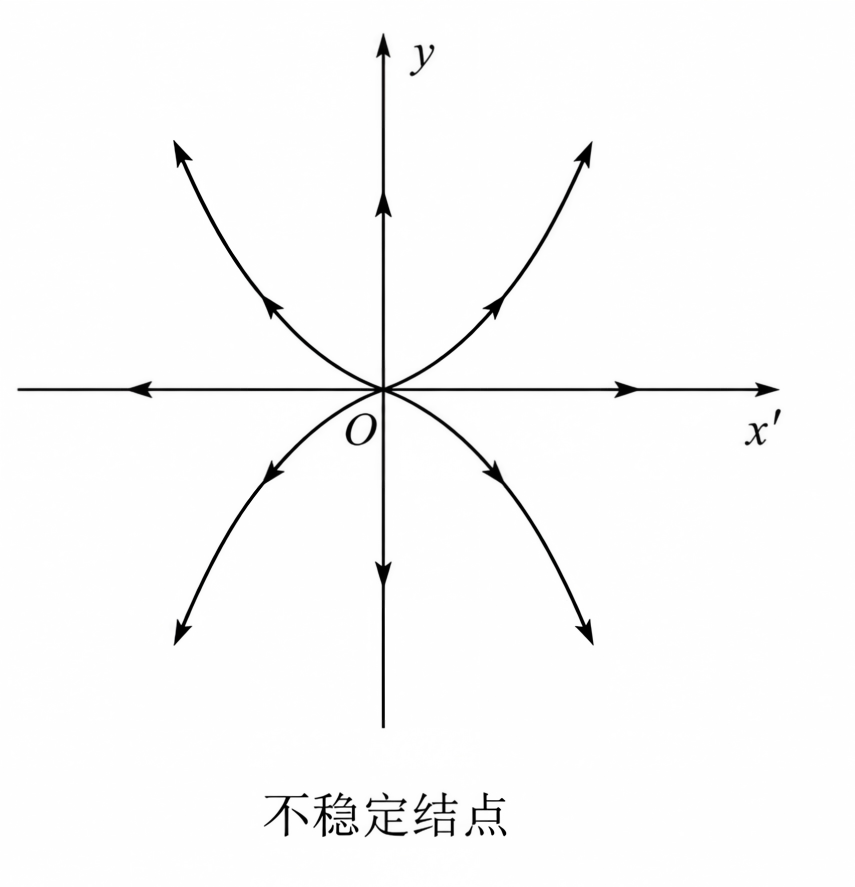
\includegraphics[width=0.4\linewidth]{figure/2.5}
	\captionof{figure}{不稳定结点}
\end{center}
\newpage

\textbf{5.}\ $q>0,p<0,p^2-4q<0$。经时间反向，原点为不稳定焦点。

\begin{center}
	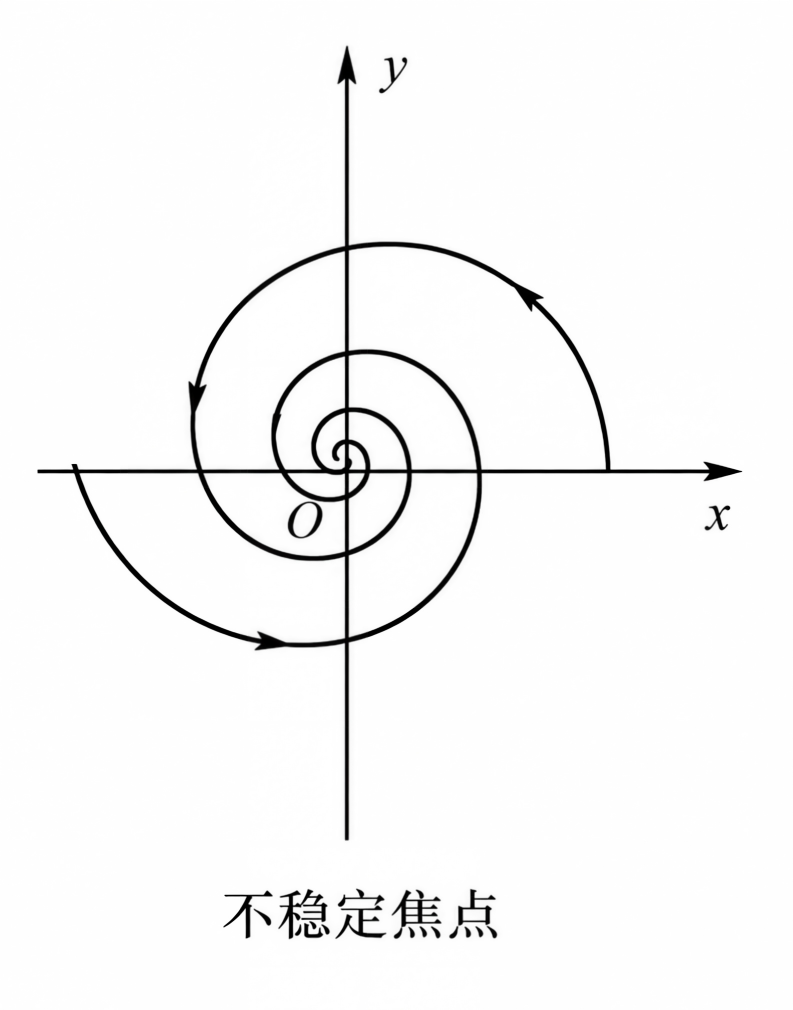
\includegraphics[width=0.4\linewidth]{figure/2.6}
	\captionof{figure}{不稳定焦点}
\end{center}

\textbf{6.}\ $q>0,p=0$。特征根为一对纯虚根；由(2.6)有 $dr/dt=0$，轨线为闭曲线，原点为中心。

\begin{center}
	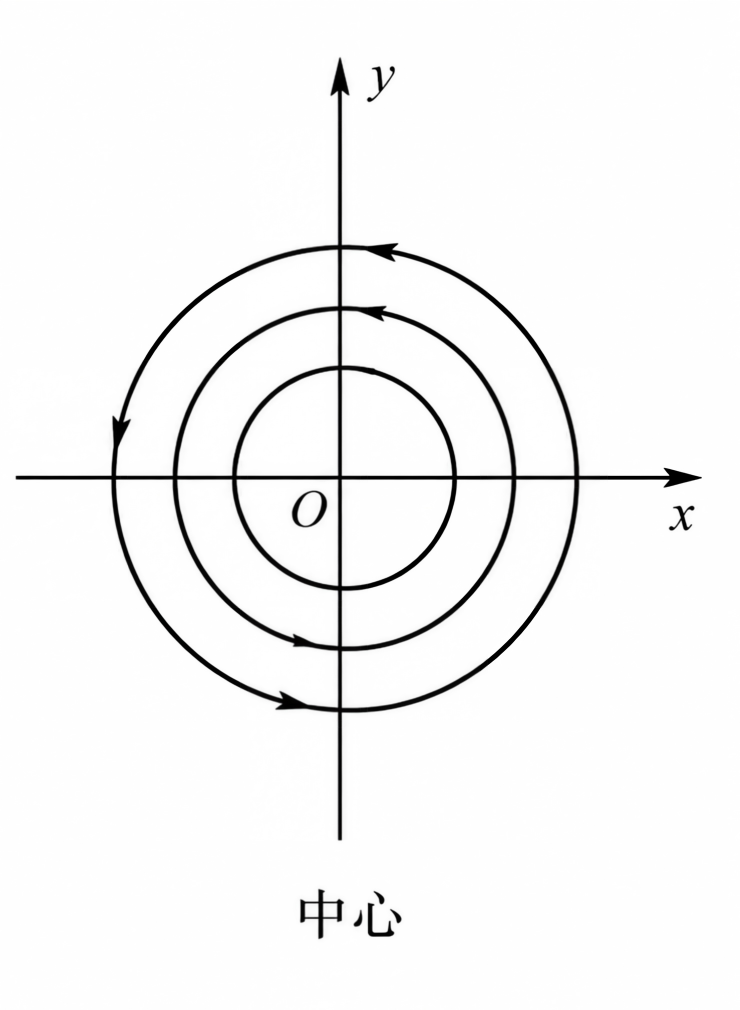
\includegraphics[width=0.4\linewidth]{figure/2.7}
	\captionof{figure}{中心}
\end{center}

\textbf{7.}\ $q>0,p>0,p^2-4q=0$。有负的重根。若最小多项式为一次式，化为 $dx'/dt=\lambda_1x'$，$dy'/dt=\lambda_1y'$，原点为稳定星形结点；若最小多项式为二次式，化为
\[
\dfrac{dx'}{dt}=\lambda_1x',\qquad
\dfrac{dy'}{dt}=\xi x'+\lambda_1y',\tag{2.8}
\]
则为稳定退化结点。
\begin{center}
	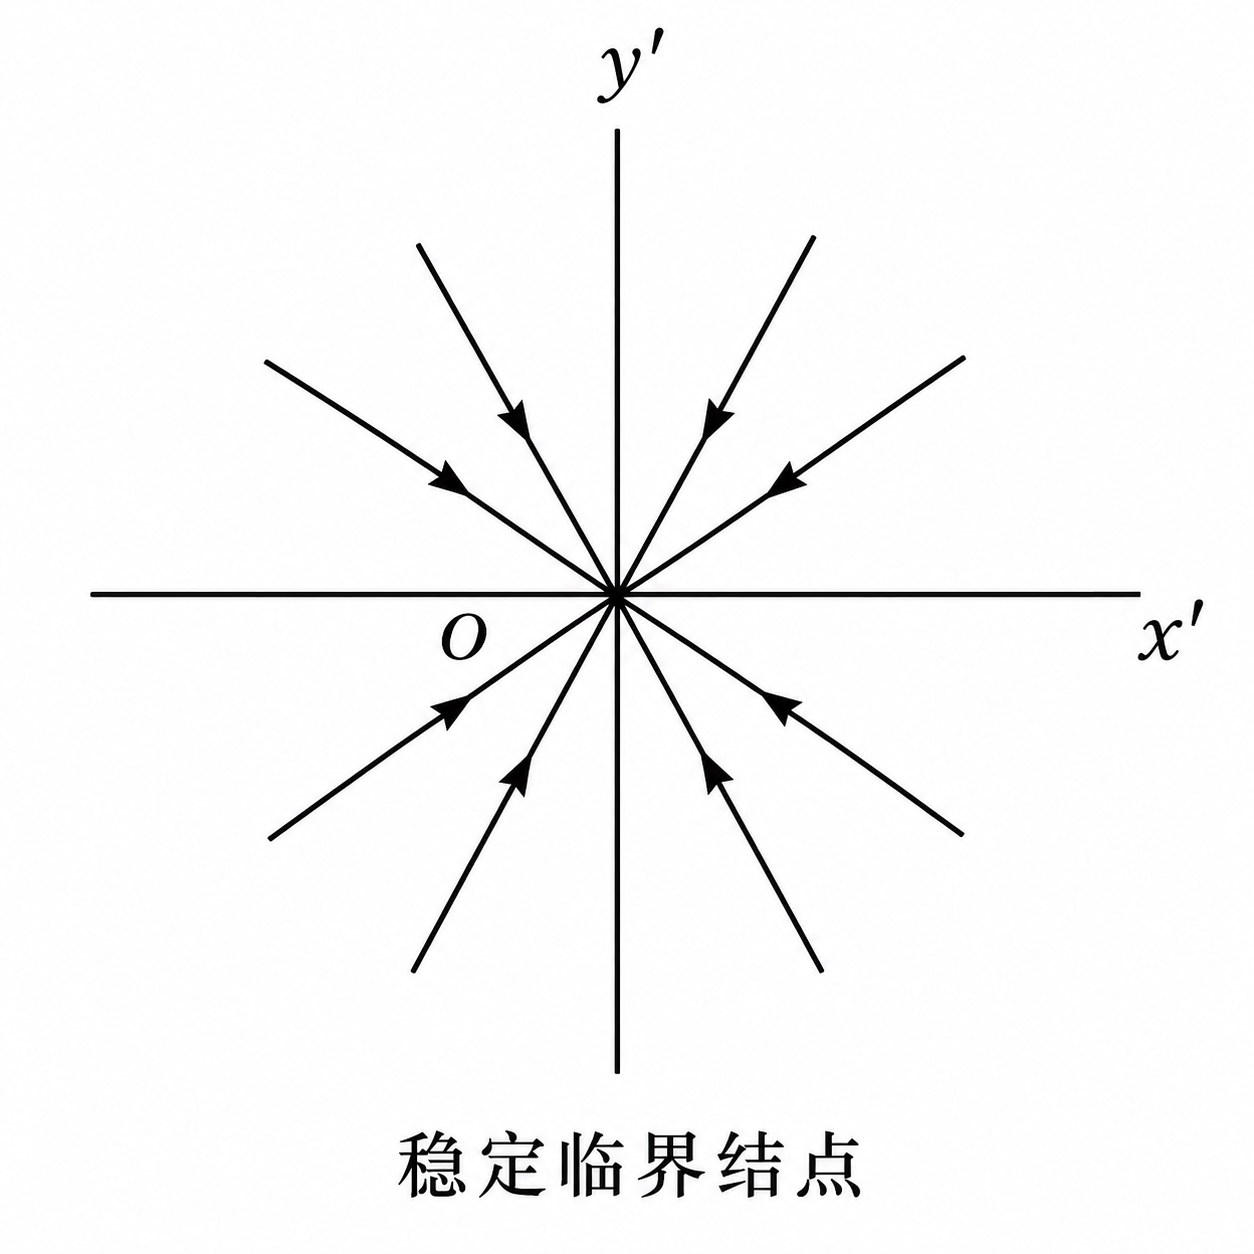
\includegraphics[width=0.4\linewidth]{figure/2.8}
	\captionof{figure}{稳定临界结点}
\end{center}



\textbf{8.}\ $q>0,p<0,p^2-4q=0$。有正的重根，轨线为第7种情形的时间反向；原点为不稳定星形结点或不稳定退化结点。
\begin{center}
	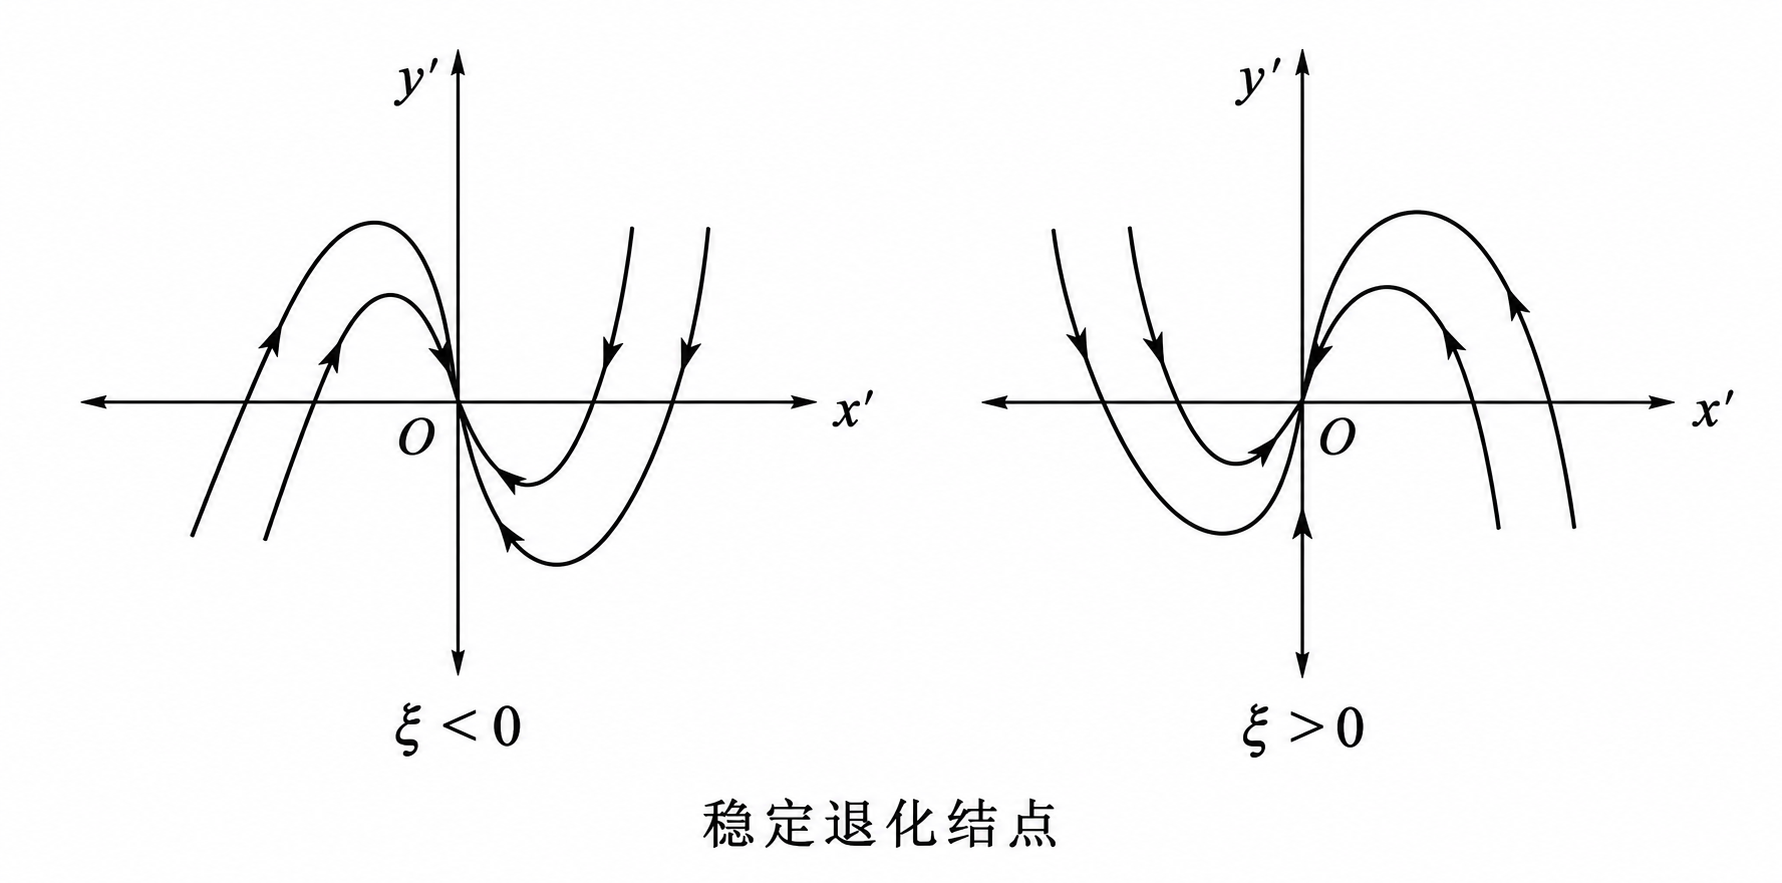
\includegraphics[width=0.47\linewidth]{figure/2.9}
	\captionof{figure}{稳定临界结点}
\end{center}
\textbf{9.}\ $q=0$。若 $a=b=c=d=0$，则平面上每一点均为奇点。若方程组中有一个方程恒为零，另一方程的零直线即为奇点的全体。若两式均不恒为零，则 $ax+by=0$ 与 $cx+dy=0$ 为同一直线，直线上的每一点均为奇点；例如在 $ac\ne0$ 时，
\[
\dfrac{dy}{dx}=\dfrac ca,\qquad ay-cx+k=0.
\]

\begin{center}
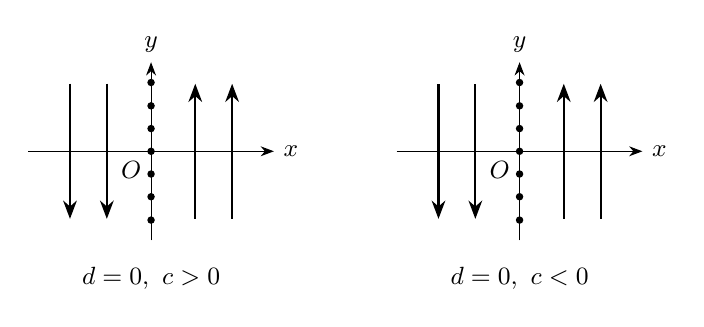
\begin{tikzpicture}[x=0.78cm,y=0.78cm,>=Stealth,font=\small]
  \begin{scope}[shift={(-3.0,0)}]
    \draw[->] (-2.0,0) -- (2.0,0) node[right] {$x$};
    \draw[->] (0,-1.45) -- (0,1.45) node[above] {$y$};
    \node[below left] at (0,0) {$O$};
    \foreach \yy in {-1.12,-.74,-.37,0,.37,.74,1.12} \fill (0,\yy) circle (1.35pt);
    \foreach \xx in {1.32,.72} \draw[->,thick] (\xx,-1.10) -- (\xx,1.10);
    \foreach \xx in {-.72,-1.32} \draw[->,thick] (\xx,1.10) -- (\xx,-1.10);
    \node[below] at (0,-1.73) {$d=0,\ c>0$};
  \end{scope}
  \begin{scope}[shift={(3.0,0)}]
    \draw[->] (-2.0,0) -- (2.0,0) node[right] {$x$};
    \draw[->] (0,-1.45) -- (0,1.45) node[above] {$y$};
    \node[below left] at (0,0) {$O$};
    \foreach \yy in {-1.12,-.74,-.37,0,.37,.74,1.12} \fill (0,\yy) circle (1.35pt);
    \foreach \xx in {-1.32,-.72} \draw[<-,thick] (\xx,-1.10) -- (\xx,1.10);
    \foreach \xx in {.72,1.32} \draw[<-,thick] (\xx,1.10) -- (\xx,-1.10);
    \node[below] at (0,-1.73) {$d=0,\ c<0$};
  \end{scope}
\end{tikzpicture}
\captionof{figure}{非孤立奇点：$d=0$}
\end{center}

\begin{center}
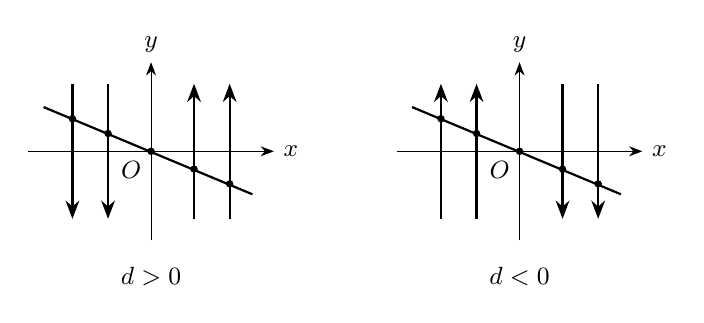
\begin{tikzpicture}[x=0.78cm,y=0.78cm,>=Stealth,font=\small]
  \begin{scope}[shift={(-3.0,0)}]
    \draw[->] (-2.0,0) -- (2.0,0) node[right] {$x$};
    \draw[->] (0,-1.45) -- (0,1.45) node[above] {$y$};
    \node[below left] at (0,0) {$O$};
    \draw[thick] (-1.75,0.72) -- (1.65,-0.70);
    \foreach \xx in {.70,1.28} \draw[->,thick] (\xx,-1.10) -- (\xx,1.10);
    \foreach \xx in {-1.28,-.70} \draw[->,thick] (\xx,1.10) -- (\xx,-1.10);
    \foreach \xx/\yy in {-1.28/.53,-.70/.29,0/0,.70/-.29,1.28/-.53} \fill (\xx,\yy) circle (1.35pt);
    \node[below] at (0,-1.73) {$d>0$};
  \end{scope}
  \begin{scope}[shift={(3.0,0)}]
    \draw[->] (-2.0,0) -- (2.0,0) node[right] {$x$};
    \draw[->] (0,-1.45) -- (0,1.45) node[above] {$y$};
    \node[below left] at (0,0) {$O$};
    \draw[thick] (-1.75,0.72) -- (1.65,-0.70);
    \foreach \xx in {-1.28,-.70} \draw[<-,thick] (\xx,1.10) -- (\xx,-1.10);
    \foreach \xx in {.70,1.28} \draw[<-,thick] (\xx,-1.10) -- (\xx,1.10);
    \foreach \xx/\yy in {-1.28/.53,-.70/.29,0/0,.70/-.29,1.28/-.53} \fill (\xx,\yy) circle (1.35pt);
    \node[below] at (0,-1.73) {$d<0$};
  \end{scope}
\end{tikzpicture}
\captionof{figure}{非孤立奇点：$d\ne0$}
\end{center}

上述图形是在 $(x',y')$ 平面画出的。回到 $(x,y)$ 平面，$x'=0,y'=0$ 是两条过原点的斜线，轨线的几何形状可能不同，但拓扑性质不变。将 $y=kx$ 代入(2.1)，可由
\[
bk^2+(a-d)k-c=0
\]
求得这两条直线的斜率。综合九种情形，可在 $(p,q)$ 平面画出分类图。

\begin{center}
\begin{tikzpicture}[x=1.0cm,y=0.86cm,>=Stealth,font=\scriptsize]
  \draw[->] (-3.2,0) -- (3.25,0) node[right] {$p$};
  \draw[->] (0,-1.85) -- (0,3.15) node[above] {$q$};
  \node[below left] at (0,0) {$O$};
  \draw[thick,domain=-3:3,smooth] plot (\x,{0.25*\x*\x});
  \node[anchor=west] at (2.06,2.38) {$p^2-4q=0$};
  \node[anchor=west] at (2.06,1.83) {稳定退化结点};
  \node at (1.38,0.83) {稳定焦点};
  \node at (1.67,0.22) {稳定结点};
  \node at (-1.42,0.83) {不稳定焦点};
  \node at (-1.75,0.22) {不稳定结点};
  \node[anchor=east] at (-2.25,1.66) {临界不稳定退化结点};
  \node[above] at (0,2.48) {中心};
  \node[below] at (0,-1.14) {鞍点};
  \node[below] at (1.92,0) {情形 9};
\end{tikzpicture}
\captionof{figure}{$(p,q)$ 平面上的奇点分类}
\end{center}

% ============================================================
%  §3  非线性方程组的奇点
% ============================================================
\section{非线性方程组的奇点}

给定微分方程组
\[
\left\{\begin{aligned}
\dfrac{dx}{dt}&=X(x,y),\\
\dfrac{dy}{dt}&=Y(x,y).
\end{aligned}\right.\tag{3.1}
\]
设 $O(0,0)$ 是其孤立奇点，且 $X,Y$ 在原点附近有足够高阶的连续偏导数。可写为
\[
\left\{\begin{aligned}
\dfrac{dx}{dt}&=X_m(x,y)+\Phi(x,y),\\
\dfrac{dy}{dt}&=Y_n(x,y)+\Psi(x,y),
\end{aligned}\right.\tag{3.2}
\]
其中 $X_m,Y_n$ 分别为 $x,y$ 的 $m,n$ 次齐次多项式，$m,n\ge1$，而
\[
\Phi=o(r^m),\qquad\Psi=o(r^n),\qquad r\to0.
\]
当 $m=n=1$ 且 $\Phi\equiv\Psi\equiv0$ 时，称为线性奇点；其余情形称为非线性奇点。焦点、结点、中心、鞍点称为初等奇点或简单奇点，其余的孤立奇点称为复杂奇点。

\begin{definition}{}{}
设 $L$ 是方程的轨线，点 $A(r,\theta)$ 是 $L$ 上的动点。若当 $r\to0$ 时有 $\theta\to\theta_0$，则称轨线 $L$ 沿固定方向 $\theta=\theta_0$ 进入奇点 $O$。
\end{definition}

\begin{definition}{}{}
设原点 $O$ 为方程组(3.1)的孤立奇点。若存在点列 $A_n=A(r_n,\theta_n)$，当 $n\to+\infty$ 时，$r_n\to0$，$\theta_n\to\theta_0$，且场向量的方向 $\alpha_n\to0$，则称 $\theta=\theta_0$ 为方程组(3.1)的特殊方向。
\end{definition}

若轨线沿方向 $\theta=\theta_0$ 进入奇点，则 $\theta=\theta_0$ 必为特殊方向；但沿特殊方向不一定有轨线进入奇点。对于鞍点和结点，相应的变换后方程有四个特殊方向；对于退化结点有两个特殊方向；对于临界结点，每个方向均为特殊方向；对中心和焦点没有特殊方向。

\begin{example}{}{nonlinear-special-direction}
讨论方程组
\[
\dfrac{dx}{dt}=-x,\qquad
\dfrac{dy}{dt}=-y+
\dfrac{x\cos\left|\ln\dfrac1{|x|}\right|}{\ln\dfrac1{|x|}}
\]
在奇点 $O$ 邻域内的轨线结构。
\end{example}
由第一个方程得 $x(t)=x(0)e^{-t}$。代入第二式可得
\[
y(t)=x(t)\left[C_2+\sin\left|\ln\dfrac1{|x(t)|}\right|\right].
\]
于是可适当选取 $t_n\to+\infty$，使 $dy/dx=y/x=C_2+1$。因而每一方向均为特殊方向；但除 $x=0$ 外，其余轨线均不沿固定方向进入奇点。

\chTwoFigurePlaceholder{2.13}

在极坐标下，设轨线与向量半径 $\theta=\theta_0$ 相交于点 $P$。若在点 $P$ 坐标向量与场向量的夹角 $\alpha_P<\pi$（$>\pi$），则称轨线与该半径正（负）侧相交。

\chTwoFigurePlaceholder{2.14}

由两条向量半径 $OA,OB$ 和弧 $\overset{\frown}{AB}$ 围成的扇形区域 $\overset{\frown}{OAB}$，若除 $O$ 外无其他奇点，$OA,OB$ 为无切线段，区域内至多有一个特殊方向，且边界方向不是特殊方向，则称为正常区域。轨线在两条边界上同向进入或同向离开该区域。

\chTwoFigurePlaceholder{2.15}
\chTwoFigurePlaceholder{2.16}

\begin{proposition}{}{}
若 $\overset{\frown}{OAB}$ 是第一类正常区域，则当 $t\to+\infty$ 时，由 $OA,OB$ 上每一点出发的轨线均进入奇点 $O$。
\end{proposition}

\begin{proposition}{}{}
若 $\overset{\frown}{OAB}$ 是第二类正常区域，则弧 $\overset{\frown}{AB}$ 上存在一点或一闭弧段，从其上出发的轨线当 $t\to+\infty$ 时均进入奇点 $O$。
\end{proposition}

研究非线性奇点附近轨线的定性结构，主要是找出所有特殊方向，再讨论沿这些方向是否有轨线进入奇点以及有多少条。令 $\alpha$ 为 $P(r,\theta)$ 处坐标向量与场向量的夹角，则
\[
\tan\alpha=\lim_{\Delta r\to0}r\dfrac{\Delta\theta}{\Delta r}
=r\dfrac{d\theta}{dr}.\tag{3.4}
\]
令 $x=r\cos\theta,y=r\sin\theta$，则
\[
\dfrac1r\dfrac{dr}{d\theta}=\dfrac{M(r,\theta)}{I(r,\theta)},\tag{3.5}
\]
其中，若 $m>n$、$m<n$、$m=n$，分别令
\[
G(\theta)=\cos\theta Y_n(\cos\theta,\sin\theta),\quad
G(\theta)=-\sin\theta X_m(\cos\theta,\sin\theta),
\]
或
\[
G(\theta)=\cos\theta Y_n(\cos\theta,\sin\theta)-\sin\theta X_m(\cos\theta,\sin\theta).\tag{3.6}
\]
由附加项的条件，在充分小的 $r$ 下，上式右端的分母除以相应的 $r^m$ 或 $r^n$ 后为 $G(\theta)+o(1)$。故特殊方向必须是示性方程 $G(\theta)=0$ 的根。

\begin{theorem}{}{}
若原点为方程组(3.1)的孤立奇点，且 $X,Y$ 在原点邻域内解析，则若有轨线进入原点，它只能螺旋形地进入或沿固定方向进入。
\end{theorem}

\section{特征根实部不为0时附加非线性项的情形}

本节研究在线性方程组的右端附加非线性项后，当特征根实部不为零时奇点附近轨线的拓扑结构和定性结构是否保持不变。给定线性方程组
\[
\left\{\begin{aligned}
\dfrac{dx}{dt}&=ax+by,\\
\dfrac{dy}{dt}&=cx+dy,
\end{aligned}\right.\tag{4.1}
\]
及方程组
\[
\left\{\begin{aligned}
\dfrac{dx}{dt}&=ax+by+\Phi(x,y),\\
\dfrac{dy}{dt}&=cx+dy+\Psi(x,y),
\end{aligned}\right.\tag{4.2}
\]
其中 $a,b,c,d$ 为实数，$\Phi(0,0)=\Psi(0,0)=0$，并引入条件：
\[
\Phi(x,y),\Psi(x,y)=o(r),\qquad r\to0,\tag{4.3}
\]
以及 $\Phi,\Psi$ 在原点小邻域内对 $x,y$ 连续可微。第二个条件还保证了解的存在唯一性。

\begin{definition}{}{}
若存在 $\delta>0$，使任一满足 $x^2(t_0)+y^2(t_0)<\delta$ 的解在 $t\to+\infty$ 时满足 $x^2(t)+y^2(t)\to0$，则称 $O(0,0)$ 为稳定吸引子；时间反向时称为不稳定吸引子。
\end{definition}

\begin{theorem}{}{}
若 $O(0,0)$ 是方程组(4.1)的稳定（不稳定）吸引子，且方程组(4.2)的附加项满足(4.3)，则 $O(0,0)$ 也是方程组(4.2)的稳定（不稳定）吸引子。
\end{theorem}

证明中可取
\[
V(x,y)=(ad-bc)(x^2+y^2)+(ay-cx)^2+(by-dx)^2.
\]
当 $ad-bc>0$ 且 $-(a+d)>0$（或小于零）时，$V(0,0)=0$，在原点外 $V(x,y)>0$，并且沿(4.1)、(4.2)的导数分别具有相应符号，故结论成立。

\begin{theorem}{}{}
若 $O(0,0)$ 是方程组(4.1)的稳定（不稳定）焦点，且条件(4.3)成立，则 $O(0,0)$ 也是方程组(4.2)的稳定（不稳定）焦点。
\end{theorem}

经非退化线性变换，若线性部分有共轭复特征根，可化为
\[
\left\{\begin{aligned}
\dfrac{dx'}{dt}&=\mu_1x'+\mu_2y'+\Phi'(x',y'),\\
\dfrac{dy'}{dt}&=-\mu_2x'+\mu_1y'+\Psi'(x',y').
\end{aligned}\right.\tag{4.4}
\]
其示性方程无实根，故原点只能为中心或焦点；再由前一结论，原点为同稳定性的焦点。

若线性部分有两个非零实特征根，经非退化线性变换可化为
\[
\left\{\begin{aligned}
\dfrac{dx'}{dt}&=\lambda_1x'+\Phi'(x',y'),\\
\dfrac{dy'}{dt}&=\lambda_2y'+\Psi'(x',y').
\end{aligned}\right.\tag{4.5}
\]
其中 $\Phi',\Psi'$ 仍满足相应的条件。

\begin{theorem}{}{}
设 $O(0,0)$ 是方程组(4.1)的正常结点，$|\lambda_2|>|\lambda_1|$。

\noindent (i) 若条件(4.3)成立，则方程组(4.5)在奇点附近的轨线都沿特殊方向 $\theta=0,\pi/2,\pi,3\pi/2$ 进入奇点；

\noindent (ii) 若附加项连续可微，则沿 $\theta=\pi/2,3\pi/2$ 各只有一条轨线进入奇点。
\end{theorem}

\begin{theorem}{}{}
设 $O(0,0)$ 是方程组(4.1)的鞍点，$\lambda_1>0>\lambda_2$。

\noindent (i) 若条件(4.3)成立，则方程组(4.5)有轨线当 $t\to+\infty$ 时沿 $\theta=\pi/2,3\pi/2$ 进入奇点；有轨线当 $t\to-\infty$ 时沿 $\theta=0,\pi$ 进入奇点，其余轨线双侧离开充分小的邻域；

\noindent (ii) 若附加项连续可微，则沿四个特殊方向各只有一条轨线进入奇点。
\end{theorem}

\begin{theorem}{}{}
设 $O(0,0)$ 是方程组(4.1)的临界结点。若方程组(4.2)中的附加项满足
\[
\Phi(x,y),\Psi(x,y)=o\bigl(r^{1+\varepsilon}\bigr),\qquad r\to0,
\]
其中 $\varepsilon>0$ 为任意小的正数，则方程组(4.2)沿任意方向 $\theta=\theta_0$ 有唯一的轨线进入奇点 $O$。
\end{theorem}

\begin{theorem}{}{}
设 $O(0,0)$ 是方程组(4.1)的退化结点。若方程组(4.2)的附加项满足上述条件，则 $O(0,0)$ 也是方程组(4.2)的退化结点。
\end{theorem}

\begin{example}{}{critical-node-counterexample}
讨论方程组
\[
\left\{\begin{aligned}
\dfrac{dx}{dt}&=-x-\dfrac{2y}{\ln(x^2+y^2)},\\
\dfrac{dy}{dt}&=-y-\dfrac{2x}{\ln(x^2+y^2)}.
\end{aligned}\right.\tag{4.6}
\]
的原点附近轨线结构。
\end{example}
令 $x=r\cos\theta,y=r\sin\theta$，则
\[
\dfrac{d\theta}{dt}=-\dfrac1{\ln r},\qquad
\dfrac{dr}{dt}=-r.\tag{4.7}
\]
于是 $r(t)=r(0)e^{-t}$，且
\[
\theta(t)-\theta(0)=\ln\ln\dfrac1{r(t)}-\ln\ln\dfrac1{r(0)}.
\]
故 $r(t)\to0$、$\theta(t)\to+\infty$；原点为焦点，而相应的线性方程的原点为临界结点。该例的附加项满足条件1、2，但不满足上述较强条件。

\begin{example}{}{degenerate-node-counterexample}
讨论方程组
\[
\left\{\begin{aligned}
\dfrac{dx}{dt}&=-x,\\
\dfrac{dy}{dt}&=-y+\dfrac{x}{\ln\dfrac1{|x|}}.
\end{aligned}\right.\tag{4.8}
\]
由 $x(t)=x(0)e^{-t}$ 得
\[
y(t)=x(t)\left[C_2+\ln\ln\dfrac1{|x(t)|}\right].
\]
所以 $x(t),y(t)\to0$，但 $y(t)/x(t)\to+\infty$。因此原点为稳定吸引子，且轨线均沿 $y$ 轴进入原点，即为退化结点；相应线性方程的原点则为临界结点。
\end{example}

% ============================================================
%  §5  特征根是一对纯虚根时附加非线性项的情形(中心和焦点判别)
% ============================================================
\section{特征根是一对纯虚根时附加非线性项的情形(中心和焦点判别)}
设线性部分的特征根为 $\pm\mu i$，$\mu>0$。经线性变换后，线性方程组及附加非线性项的方程组分别为
\[
\dfrac{dx'}{dt}=\mu y',\qquad \dfrac{dy'}{dt}=-\mu x',
\tag{5.1}
\]
\[
\dfrac{dx'}{dt}=\mu y'+\Phi'(x',y'),\qquad
\dfrac{dy'}{dt}=-\mu x'+\Psi'(x',y').
\tag{5.2}
\]
其中 $\Phi',\Psi'$ 仍满足本章第4节的附加项条件。

\begin{theorem}{}{pure-imaginary}
在上述条件下，原点 $O$ 或为中心，或为焦点，或为中心焦点。
\end{theorem}

\begin{example}{}{focus-example}
讨论方程组
\[
\dfrac{dx}{dt}=-y-x(x^2+y^2),\qquad
\dfrac{dy}{dt}=x-y(x^2+y^2).
\tag{5.3}
\]
令 $x=r\cos\theta,\ y=r\sin\theta$，得
\[
\dfrac{d\theta}{dt}=1,\qquad \dfrac{dr}{dt}=-r^3.
\]
故
\[
\theta=\theta_0+t,\qquad
r=\left(2t+\dfrac1{r^2(0)}\right)^{-\frac12}.
\]
原点为稳定焦点。
\end{example}

\begin{example}{}{centre-focus-example}
讨论方程组
\[
\begin{aligned}
\dfrac{dx}{dt}&=-y+x(x^2+y^2)^k
 \sin\dfrac{\pi}{\sqrt{x^2+y^2}},\\
\dfrac{dy}{dt}&=x+y(x^2+y^2)^k
 \sin\dfrac{\pi}{\sqrt{x^2+y^2}}.
\end{aligned}
\tag{5.4}
\]
极坐标方程为
\[
\dfrac{d\theta}{dt}=1,\qquad
\dfrac{dr}{dt}=r^{2k+1}\sin\dfrac{\pi}{r}.
\]
圆周 $r=1/n\ (n=1,2,\ldots)$ 都是闭轨线；相邻圆周之间又有非闭轨线。因此原点为中心焦点。
\end{example}

\subsection*{中心和焦点的判别法一}

\begin{lemma}{}{periodic-integral}
若连续函数 $h(x)$ 以 $l$ 为周期，则
\[
\int_0^x h(\xi)\,d\xi=gx+\varphi(x),\qquad
g=\dfrac1l\int_0^l h(\xi)\,d\xi,
\]
其中 $\varphi(x+l)=\varphi(x)$。
\end{lemma}

在极坐标中，方程组可写为
\[
\dfrac{d\theta}{dt}=-\mu+Q(r,\theta),\qquad
\dfrac{dr}{dt}=rR(r,\theta),
\tag{5.5}
\]
从而
\[
\dfrac{dr}{d\theta}
 =R_2(\theta)r^2+R_3(\theta)r^3+\cdots .
\tag{5.6}
\]
这里 $R_i(\theta)$ 都以 $2\pi$ 为周期。取初值 $r(0,c)=c$，其解析解为
\[
r(\theta,c)=r_1(\theta)c+r_2(\theta)c^2+\cdots ,
\tag{5.8}
\]
其中
\[
r_1=1,\qquad r_2=\int_0^\theta R_2(s)\,ds,\qquad
r_3=\int_0^\theta\bigl[R_3(s)+2R_2(s)r_2(s)\bigr]\,ds .
\]
依引理可写成 $r_i=g_i\theta+\varphi_i(\theta)$。若所有 $g_i=0$，则原点为中心；若 $g_m$ 是第一个非零数，则原点为焦点，且其稳定性由 $g_m$ 的符号决定。

\subsection*{中心和焦点的判别法二}

设
\[
\dfrac{dx}{dt}=y+\sum_{k=2}^{\infty}\Phi_k,\qquad
\dfrac{dy}{dt}=-x+\sum_{k=2}^{\infty}\Psi_k.
\tag{5.16}
\]
寻求形式幂级数
\[
F=x^2+y^2+\sum_{k=3}^{\infty}F_k
\]
使得沿轨线 $dF/dt=0$。比较齐次项可得递推关系
\[
\begin{aligned}
xF_{n,y}-yF_{n,x}
={}&2(x\Phi_{n-1}+y\Psi_{n-1})\\
&+\sum_{k=3}^{n-1}
 \bigl(\Phi_{n-k+1}F_{k,x}+\Psi_{n-k+1}F_{k,y}\bigr).
\end{aligned}
\tag{5.18}
\]
若各级方程均可解，则原点为中心；否则，设第一次出现不相容条件时得到
\[
\dfrac{d}{dt}(x^2+y^2+F_3+\cdots+F_{2m})
 =-\lambda r^{2m}+O(r^{2m+1}),
\tag{5.26}
\]
则 $\lambda>0$ 时原点为稳定焦点，$\lambda<0$ 时为不稳定焦点。

若方程组关于一条坐标轴具有镜像对称性，例如
\[
Y(-x,y)=Y(x,y),\qquad X(-x,y)=-X(x,y),
\]
则原点为中心。

对于二次系统
\[
\begin{aligned}
\dfrac{dx}{dt}&=-y+a_{20}x^2+a_{11}xy+a_{02}y^2,\\
\dfrac{dy}{dt}&=x+b_{20}x^2+b_{11}xy+b_{02}y^2,
\end{aligned}
\tag{5.28}
\]
令
\[
\begin{gathered}
A=a_{20}+a_{02},\quad B=b_{20}+b_{02},\\
\alpha=a_{11}+2b_{02},\quad \beta=b_{11}+2a_{20},\\
\gamma=b_{20}A^3-(a_{20}-b_{11})A^2B
 +(b_{02}-a_{11})AB^2-a_{02}B^3,\\
\delta=a_{02}^2+b_{20}^2+a_{02}A+b_{20}B.
\end{gathered}
\tag{5.30}
\]
则相应的焦点量为
\[
\begin{aligned}
W_1&=A\alpha-B\beta,\\
W_2&=[\beta(5A-\beta)+\alpha(5B-\alpha)]\gamma,\\
W_3&=(A\beta+B\alpha)\gamma\delta.
\end{aligned}
\tag{5.29}
\]
原点为 $k$ 阶细焦点 $(k=1,2,3)$，当且仅当此前的焦点量为零而 $W_k\ne0$；$W_k<0$ 时稳定，$W_k>0$ 时不稳定。原点为中心当且仅当下列三组条件之一成立：
\[
\begin{array}{ll}
(1)&A\alpha-B\beta=\gamma=0;\\
(2)&\alpha=\beta=0;\\
(3)&5A-\beta=5B-\alpha=\delta=0.
\end{array}
\]

% ============================================================
%  §6  奇点的几何分类
% ============================================================
\section{奇点的几何分类}
本节讨论非中心孤立奇点邻域内轨线的几何形状。

\begin{theorem}{}{no-closed-orbit}
设 $O$ 为非中心孤立奇点，则存在充分小的圆盘 $S_\delta$，使其中除 $O$ 外没有奇点，也没有包围 $O$ 的整条闭轨线。
\end{theorem}

\chTwoFigurePlaceholder{2.28}

\begin{theorem}{}{semi-orbits}
在奇点 $O$ 的任一充分小邻域中，至少有两条半轨线在 $t\to+\infty$ 或 $t\to-\infty$ 时趋于 $O$。
\end{theorem}

\begin{theorem}{}{local-orbits}
可取充分小的 $S_\delta$，使其中每一条正、负半轨线或者趋于 $O$，或者离开 $S_\delta$。
\end{theorem}

\chTwoFigurePlaceholder{2.29}

一条经过邻域内点的轨线按两端的性状分为三种：一端进入而另一端离开 $O$ 的称为双曲型；两端均离开 $O$ 的称为双曲扇形型；两端均进入 $O$ 的称为椭圆型。由两条趋于 $O$ 的半轨线及其间的弧段所围成的区域称为曲边扇形。

\chTwoFigurePlaceholder{2.30}

\begin{theorem}{}{sector-finiteness}
在充分小的邻域内，双曲扇形、双曲椭圆扇形及椭圆扇形的数目均为有限。
\end{theorem}

因此，孤立奇点邻域内的曲边扇形只有五种：椭圆扇形、双曲扇形、双曲椭圆扇形、双曲型扇形和双曲椭圆型扇形。

\chTwoFigurePlaceholder{2.31}

设 $e$ 为椭圆扇形数，$h$ 为双曲扇形和双曲椭圆扇形的总数，奇点的指数为 $I$，则 Bendixson 公式为
\[
I=1+\dfrac{e-h}{2}.
\]

\begin{definition}{}{separatrix}
若趋于奇点的半轨线的任何充分小邻域内都含有不趋于该奇点的轨线，则称此半轨线为分界线。
\end{definition}

\begin{example}{}{geometric-classification}
讨论方程组
\[
\dfrac{dx}{dt}=-x^2+2xy,\qquad
\dfrac{dy}{dt}=\dfrac32y^2-\dfrac12x^2
\]
在原点邻域内的轨线结构。
\end{example}

% ============================================================
%  §7  有零特征根时附加非线性项的情形
% ============================================================
\section{有零特征根时附加非线性项的情形}
+本节设线性部分至少有一个零特征根，且线性项不全为零。

先设一个特征根为零，另一个不为零。经线性变换后可写为
\[
\dfrac{dx}{dt}=P_2(x,y),\qquad
\dfrac{dy}{dt}=y+Q_2(x,y),
\tag{7.1}
\]
其中 $P_2,Q_2$ 的展开式从二次项开始。由
\[
y+Q_2(x,y)=0
\]
可解得 $y=\varphi(x)$，且 $\varphi(0)=\varphi'(0)=0$。设
\[
\varphi(x)=a_mx^m+\cdots,\qquad a_m\ne0.
\]

\begin{theorem}{}{one-zero-eigenvalue}
对于方程组(7.1)，有：

\noindent (i) 当 $m$ 为奇数、$a_m>0$ 时，原点为不稳定结点；

\noindent (ii) 当 $m$ 为奇数、$a_m<0$ 时，原点为鞍点，具有四条分界线；

\noindent (iii) 当 $m$ 为偶数时，原点为鞍结点；它有两条切于非零特征方向的分界线和一个抛物扇形，另有两个双曲扇形。
\end{theorem}

\chTwoFigurePlaceholder{2.32}
\chTwoFigurePlaceholder{2.33}
\chTwoFigurePlaceholder{2.34}
\chTwoFigurePlaceholder{2.35}

现设两个特征根均为零，但线性部分不为零。经过可逆变换，方程组可化为
\[
\dfrac{dx}{dt}=y,\qquad \dfrac{dy}{dt}=\overline Q_2(x,y).
\tag{7.6}
\]
其右端可写为
\[
\dfrac{dx}{dt}=y,\qquad
\dfrac{dy}{dt}=a_kx^k[1+h(x)]
+b_nx^ny[1+g(x)]+y^2p(x,y),
\tag{7.7}
\]
其中 $h(0)=g(0)=0$，$a_k\ne0$。

令 $k=2m+1$。若 $b_n=0$ 或 $n>m$，则
\[
a_{2m+1}<0\ \Longrightarrow\ \text{中心或焦点},\qquad
a_{2m+1}>0\ \Longrightarrow\ \text{鞍点}.
\]
当 $b_n\ne0,\ n<m$ 时，$a_{2m+1}>0$ 仍为鞍点；当 $a_{2m+1}<0$ 时，$n$ 为偶数对应结点，$n$ 为奇数对应一个椭圆扇形和一个双曲扇形。

\chTwoFigurePlaceholder{2.36}
\chTwoFigurePlaceholder{2.37}
\chTwoFigurePlaceholder{2.38}
\chTwoFigurePlaceholder{2.39}
\chTwoFigurePlaceholder{2.40}
\chTwoFigurePlaceholder{2.41}
\chTwoFigurePlaceholder{2.42}
\chTwoFigurePlaceholder{2.43}
\chTwoFigurePlaceholder{2.44}
\chTwoFigurePlaceholder{2.45}

若 $n=m$，令
\[
\lambda=b_n^2+4(m+1)a_{2m+1}.
\]
上述分类中相应条件改为由 $\lambda$ 的符号判定。综上可得：当 $a_{2m+1}>0$ 时为鞍点；当 $a_{2m+1}<0$ 且 $b_n=0$，或 $n>m$，或 $n=m,\lambda<0$ 时为中心或焦点；当 $a_{2m+1}<0$ 且 $n\le m,\lambda\ge0$ 时，按 $n$ 的奇偶分别为结点或由一个椭圆扇形和一个双曲扇形组成的奇点。

\chTwoFigurePlaceholder{2.46}
\chTwoFigurePlaceholder{2.47}
\chTwoFigurePlaceholder{2.48}
\chTwoFigurePlaceholder{2.49}

\begin{theorem}{}{even-k}
当 $k=2m$ 时，若 $b_n=0$，则原点为退化奇点；若 $b_n\ne0$ 且 $n\ge m$，则原点为鞍结点。
\end{theorem}

\chTwoFigurePlaceholder{2.50}
\chTwoFigurePlaceholder{2.51}

实际计算时，先由 $y+P_2(x,y)=0$ 求出 $y=\varphi(x)$，再计算
\[
\psi(x)=Q_2(x,\varphi(x)),\qquad
\delta(x)=P_{2x}(x,\varphi(x))+Q_{2y}(x,\varphi(x)).
\]
由 $\psi,\delta$ 展开式中的最低次非零项，即可确定上述判别中的 $k,m,a_k,n,b_n$。

\begin{example}{}{zero-eigenvalue-example1}
讨论方程组
\[
\dfrac{dx}{dt}=x(-y+y^2+3xy),\qquad
\dfrac{dy}{dt}=3x+y-x^2+y^3+3xy^2.
\]
原点可化为(7.1)的类型，并由定理 \ref{thm:one-zero-eigenvalue} 判定其局部轨线结构。
\end{example}

\begin{example}{}{zero-eigenvalue-example2}
讨论方程组
\[
\dfrac{dx}{dt}=y-\dfrac12xy-3x^3,\qquad
\dfrac{dy}{dt}=-y\left(x+\dfrac32y\right).
\]
它在原点邻域内的图形为图2.52所示的类型。
\end{example}

\chTwoFigurePlaceholder{2.52}

\begin{example}{}{zero-eigenvalue-example3}
讨论方程组
\[
\dfrac{dx}{dt}=y+y^2-x^3,\qquad
\dfrac{dy}{dt}=3x^2y+y^3-3x^5.
\]
其原点邻域的轨线结构如图2.53所示。
\end{example}

\chTwoFigurePlaceholder{2.53}
\chTwoFigurePlaceholder{2.54}

% ============================================================
%  习题和参考文献
% ============================================================
\section*{习题和参考文献}
\subsection*{习题}

\begin{enumerate}
\item 试画出第2节情形9(iii)的草图。
\item 试讨论下列非线性方程组在奇点 $O(0,0)$ 邻域轨线的结构，并画出草图：
\[
\begin{array}{ll}
\text{(i)}&
\dfrac{dx}{dt}=-x+e^{-y}-1,\qquad
\dfrac{dy}{dt}=1-e^{x+y};\\[4pt]
\text{(ii)}&
\dfrac{dx}{dt}=xy,\qquad
\dfrac{dy}{dt}=y^2+x^4;\\[4pt]
\text{(iii)}&
\dfrac{dx}{dt}=-x^6,\qquad
\dfrac{dy}{dt}=y^3-x^4y.
\end{array}
\]
\item 试证例题3.1，4.1，4.2，4.3中的附加项满足条件1和条件2，但不满足条件 $1^\ast$。
\item 试证定理4.5仍真，若将条件 $1^\ast$ 换成条件 $1^{\ast\ast}$：
\[
|\Phi(x,y)|,\ |\Psi(x,y)|<\eta(r),\qquad r\le r_1,
\]
其中 $\eta(r)\in C^0(0\le r\le r_1)$，$\eta(r)=o(r)$ $(r\to0)$，且
\[
\int_0^{r_1}\dfrac{\eta(r)}{r^2}\,dr<+\infty.
\]
\item 试讨论，若将条件 $1^\ast$ 换成条件 $1^{\ast\ast}$，定理4.6是否仍真。
\item 试用第一判别法和第二判别法来判定方程组
\[
\dfrac{dx}{dt}=-y+xy+2y^2,\qquad
\dfrac{dy}{dt}=x+3x^2+y^3
\]
的奇点 $O(0,0)$ 是中心或焦点。
\item 试证若 $O(0,0)$ 是方程组(5.16)的焦点，则第一判别法中使 $g_n\ne0$ 的最小正整数 $n$ 与第二判别法中使(5.19)无解的最小偶数 $2m$ 之间有关系 $2m=n+1$。
\item 试讨论下列非线性方程组在奇点 $O(0,0)$ 邻域轨线的结构，并画出草图：
\[
\begin{array}{ll}
\text{(i)}&
\dfrac{dx}{dt}=-4x^2+2xy,\qquad
\dfrac{dy}{dt}=y^3-2x^3+x^4;\\[4pt]
\text{(ii)}&
\dfrac{dx}{dt}=2x^3+x^2y+x^2,\qquad
\dfrac{dy}{dt}=2xy^2-x^3+2y^2.
\end{array}
\]
\item 试讨论下列非线性方程组在奇点 $O(0,0)$ 邻域轨线的结构，并画出草图：
\[
\dfrac{dx}{dt}=x(2y+x),\qquad
\dfrac{dy}{dt}=x+2xy+y^2.
\]
\end{enumerate}

\subsection*{参考文献}

\begin{enumerate}
\item Вайсборд, С.\ М., Об эквивалентности систем дифференциальных уравнений в окрестности особой точки, \textit{Научные Доклады Высшей Школы, Физ-Матем. Науки}, 1958, 1, 37--42.
\item Lohn, R., Über singuläre Punkte gewöhnlicher Differentialgleichungen, \textit{Math. Ztscher.}, 44(1939), 4, 507--535.
\item 张锦炎，常微分方程几何理论和分支问题，北京大学出版社，1981。
\item 胡钦训，陆毓勋，高次奇点在不定号情形下的定性分析，\textit{北京工业学院学报}，1981，2，1--16。
\item Гробман, Д., О гомеоморфизме систем дифференциальных уравнений, \textit{ДАН СССР}, 128(1959), 880--881.
\item Hartman, P., On the local linearization of differential equations, \textit{Proc. A. M. S.}, 14(1963), 568--573.
\item Sternberg, S., Lectures on differential geometry, Prentice-Hall, 1964.
\item Ляпунов, А.\ М., Исследование одного из особенных случаев задачи об устойчивости движения, \textit{Мат. Сб.}, 17(1893), 2.
\item Альмухамедов, М.\ И., О числе возможных типов особых точек для систем обыкновенных дифференциальных уравнений с $n$-переменными, \textit{Казань, Изв. Физматем. общества}(3), 8(1936--1937), 23--29.
\item ---，О проблеме центра，---，8(1936--1937)，29--37。
\item 廖山涛，常微系统的结构稳定性及一些相关的问题，\textit{计算机应用与应用数学}，7(1978)，52--64。
\item Dulac, H., Détermination et intégration d'une certaine classe d'équations différentielles ayant pour point singulier un centre, \textit{Bull. Sc. Math.} (2), 32(1908), 230--252.
\item Kapteyn, W., Over de middelpunten de integraalkrommen van differentiaalvergelijkingen van de eerste orde en den eersten graad, \textit{Koninkl. Nederland. Akad.}, 19(1911), 1446--1457.
\item ---，Nieuw onderzoek omtrent de middelpunten der integralen van differentiaalvergelijkingen van de eerste orde en den eersten graad，\textit{Koninkl. Nederland. Akad.}, 20(1912), 1354--1365; 21(1912), 27--33.
\item Сахарников, Н.\ А., Об условиях фроммера существования центра, \textit{ПММ}, 12:5(1948), 669--670.
\item Сибирский, К.\ С., Алгебраические инварианты дифференциальных уравнений и матриц, Кишинев, Штиинца, 1976, 131--140.
\item Баутин, Н.\ Н., О числе предельных циклов, появляющихся при изменении коэффициентов из состояния равновесия типа фокуса или центра, \textit{Мат. Сб.}, 30(72), 1952, 1, 181--196.
\item 葉元勋，刘海全，微分方程公式的机器推导(III)，\textit{科学通报}，7(1981)，388--391。
\item 李承治，关于平面二次系统的两个问题，\textit{中国科学，A辑}，12(1982)，1087--1096。
\item 叶澄谦，В.\ И.\ Зубов著“A.\ М.\ Ляпунов方法及其应用”一书中两个错误定理的修正，\textit{南京大学学报}，1(1963)，67--70。
\item 黄文灿，Cauchy 运动和极小集合，\textit{数学学报}，22(1979)，249--252。
\item 丁同仁，关于 Ляпунов 第一临界情形积分曲线的拓扑分布，见第一章文献[3]，138--146。
\item Андронов, А.\ А., Леонтович, Е.\ А., Гордон, И.\ И., Майер, А.\ Г., Качественная теория динамических систем второго порядка, Изд. Наука, 1966, 241--249, 377--410.
\item Frömmer, M., Die Integralkurven einer gewöhnlichen Differentialgleichung erster Ordnung in der Umgebung rationaler Unbestimmtheitsstellen, \textit{Math. Annulen}, 99(1928), 222--272.
\item Андреев, А.\ Ф., Особые точки дифференциальных уравнений, Минск, Высшая школа, 1979.
\end{enumerate}

\endinput

%
%% 第三章  平面奇点指数
%% ============================================================
%  chapter03.tex — 第三章 平面奇点指数
%  对应原书第三章。
%  引入向量场旋转数与奇点指数的拓扑不变量，并给出指数计算的
%  代数公式（Cauchy 指标、Bendixson 公式等）。
% ============================================================

\newcommand{\chThreeFigurePlaceholder}[1]{%
  \begin{center}
    \fbox{\parbox{0.72\textwidth}{\centering\vspace{2.7cm}图~#1\\（图片占位）\vspace{2.7cm}}}
  \end{center}%
}

\setchapterimage{}
\setchapterintro{}
\chapter{平面奇点指数}

% ============================================================
%  §1  连续向量场的旋转数
% ============================================================
\section{连续向量场的旋转数}

给定平面 $\mathbb{R}^2$ 上的连续向量场
\[
  A(x,y)=\bigl(X(x,y),Y(x,y)\bigr),\qquad (x,y)\in\mathbb{R}^2.
\]
设 $\mathscr{L}\subset\mathbb{R}^2$ 是一条有向的闭分段光滑曲线，且
$A(x,y)$ 在 $\mathscr{L}$ 上非退化，即
\[
  X^2(x,y)+Y^2(x,y)\ne0,\qquad (x,y)\in\mathscr{L}.
\]
作单位化映射
\[
  T(x,y)=\dfrac{A(x,y)}{\lVert A(x,y)\rVert}
  =\left(
    \dfrac{X(x,y)}{\sqrt{X^2(x,y)+Y^2(x,y)}},
    \dfrac{Y(x,y)}{\sqrt{X^2(x,y)+Y^2(x,y)}}
  \right).
\]
它将 $\mathscr{L}$ 映入单位圆周。映射 $T$ 的度 $\mu(T,\mathscr{L})$
称为向量场 $A$ 沿 $\mathscr{L}$ 的\emph{旋转数}，记为
\[
  \gamma(A,\mathscr{L})=\mu(T,\mathscr{L}). \tag{1.1}
\]

若 $A(x,y)$ 光滑，则
\[
  \gamma(A,\mathscr{L})
  =\dfrac{1}{2\pi}\oint_{\mathscr{L}}
  \mathrm{d}\arctan\dfrac{Y}{X}. \tag{1.2}
\]

设 $D\subset\mathbb{R}^2$ 是有界闭区域，其边界为
\[
  \partial D=\bigcup_{i=1}^n\partial D_i,
\]
并取 $\partial D_i$ 的正向，使区域在行进方向的左侧。定义
\[
  \gamma(A,\partial D)=\sum_{i=1}^n\gamma(A,\partial D_i).
\]

\chThreeFigurePlaceholder{3.1}
\chThreeFigurePlaceholder{3.2}
\chThreeFigurePlaceholder{3.3}

\noindent\textbf{性质~1}\quad
设 $D_1,D_2$ 是两个内部没有公共点的有界闭区域，且 $A$ 在
$\partial D_1\cup\partial D_2$ 上非退化，则
\[
  \gamma(A,\partial(D_1\cup D_2))
  =\gamma(A,\partial D_1)+\gamma(A,\partial D_2). \tag{1.3}
\]

\noindent\textbf{性质~2}\quad
若 $A$ 在有界闭区域 $D$ 上连续且非退化，则
\[
  \gamma(A,\partial D)=0.
\]
事实上，当 $D$ 单连通时，上式由连续向量场的光滑逼近即得。一般地，
设 $\partial D=\bigcup_{i=1}^n\partial D_i$，将 $D$ 分成
$n-1$ 个单连通区域 $G_i$，如图~3.4 所示。由单连通情形和性质~1，
便有
\[
  \gamma(A,\partial D)=\sum_{i=1}^{n-1}\gamma(A,\partial G_i)=0.
\]

\chThreeFigurePlaceholder{3.4}

\begin{definition}{}{homotopy-vector-field}
设 $D\subset\mathbb{R}^2$ 是有界闭区域，$A_0(x,y),A_1(x,y)$
是 $\partial D$ 上的连续、非退化向量场。若存在依赖于参数
$\lambda$ 的连续向量场，也可看成连续映射
\[
  A(x,y,\lambda):\partial D\times[0,1]\longrightarrow\mathbb{R}^2,
\]
且
\[
  A(x,y,0)=A_0(x,y),\qquad A(x,y,1)=A_1(x,y),
\]
并且当 $(x,y)\in\partial D$、$\lambda\in[0,1]$ 时
$A(x,y,\lambda)$ 恒不为零，则称 $A(x,y,\lambda)$ 为从
$A_0(x,y)$ 到 $A_1(x,y)$ 的连续形变；此时称 $A_0(x,y)$ 与
$A_1(x,y)$ 同伦。
\end{definition}

\begin{theorem}{}{homotopy-transitivity}
若 $A_0(x,y),A_1(x,y)$ 都与 $A_*(x,y)$ 同伦，则
$A_0(x,y)$ 与 $A_1(x,y)$ 也同伦。
\end{theorem}

\begin{proof}
设从 $A_i(x,y)$ 到 $A_*(x,y)$ 的连续、非退化形变分别为
$\overline{A}_i(x,y,\lambda)$，$i=0,1$。令
\[
  A(x,y,\lambda)=
  \begin{cases}
    \overline{A}_0(x,y,2\lambda),&0\leq\lambda\leq\dfrac12,\\
    \overline{A}_1(x,y,2-2\lambda),&\dfrac12<\lambda\leq1,
  \end{cases}
\]
则 $A(x,y,\lambda)$ 即为从 $A_0(x,y)$ 到 $A_1(x,y)$ 的连续、
非退化形变。
\end{proof}

\noindent\textbf{性质~3}\quad
设 $D\subset\mathbb{R}^2$ 是有界闭区域，则 $\partial D$ 上的同伦
向量场有相同的旋转数。事实上，$\gamma(A(x,y,\lambda),\partial D)$
一方面为整数，另一方面关于 $\lambda$ 连续，故只能为常数。

\begin{theorem}{}{same-rotation-nonopposite}
设 $D\subset\mathbb{R}^2$ 是有界闭区域，在 $\partial D$ 上有两个
非退化、连续向量场 $A_0(x,y)$ 和 $A_1(x,y)$。若对一切
$(x,y)\in\partial D$，$A_0(x,y)$ 和 $A_1(x,y)$ 的方向恒不相反，即
\[
  \dfrac{A_0(x,y)}{\lVert A_0(x,y)\rVert}
  \ne-\dfrac{A_1(x,y)}{\lVert A_1(x,y)\rVert},
  \qquad (x,y)\in\partial D,
\]
则
\[
  \gamma(A_0,\partial D)=\gamma(A_1,\partial D). \tag{1.5}
\]
\end{theorem}

\begin{proof}
构造连续形变
\[
  A(x,y,\lambda)=(1-\lambda)A_0(x,y)+\lambda A_1(x,y),
  \qquad (x,y)\in\partial D,\quad 0\leq\lambda\leq1.
\]
若它在某点退化，则
\[
  (1-\lambda_0)A_0(x_0,y_0)=-\lambda_0A_1(x_0,y_0),
\]
从而 $A_0(x_0,y_0)$ 和 $A_1(x_0,y_0)$ 的方向相反，矛盾。因此该形变
非退化，结论由性质~3 得证。
\end{proof}

\begin{definition}{}{continuous-perturbation}
设 $D\subset\mathbb{R}^2$ 是有界闭区域，设 $A_0(x,y)$ 是
$\partial D$ 上的连续、非退化向量场。向量场
$\Delta A_0(x,y)$ 称作 $A_0(x,y)$ 的连续微小扰动，若
$\Delta A_0(x,y)$ 在 $\partial D$ 上连续，且
\[
  \lVert\Delta A_0(x,y)\rVert<\lVert A_0(x,y)\rVert,
  \qquad (x,y)\in\partial D.
\]
\end{definition}

\begin{theorem}{}{small-perturbation-rotation}
设 $D\subset\mathbb{R}^2$ 是有界闭区域。若 $A_0(x,y)$ 是
$\partial D$ 上的连续、非退化向量场，$\Delta A_0(x,y)$ 是
$A_0(x,y)$ 的连续微小扰动，令
\[
  A_1(x,y)=A_0(x,y)+\Delta A_0(x,y),
\]
则 $A_1(x,y)$ 在 $\partial D$ 上也非退化，且
\[
  \gamma(A_0,\partial D)=\gamma(A_1,\partial D). \tag{1.6}
\]
\end{theorem}

\begin{proof}
构造从 $A_0(x,y)$ 到 $A_1(x,y)$ 的连续形变
\[
  A(x,y,\lambda)=A_0(x,y)+\lambda\Delta A_0(x,y),
  \qquad (x,y)\in\partial D,\quad0\leq\lambda\leq1.
\]
由微小扰动的定义，
\[
  \lVert A(x,y,\lambda)\rVert
  \geq\lVert A_0(x,y)\rVert-\lambda\lVert\Delta A_0(x,y)\rVert
  >(1-\lambda)\lVert\Delta A_0(x,y)\rVert\geq0.
\]
故 $A_0(x,y)$ 与 $A_1(x,y)$ 同伦，由性质~3 即得式~(1.6)。
\end{proof}

% ============================================================
%  §2  平面奇点指数
% ============================================================
\section{平面奇点指数}

对于由连续向量场
\[
  A(x,y)=\bigl(X(x,y),Y(x,y)\bigr)
\]
所确定的平面微分方程
\[
  \dfrac{\mathrm{d}x}{\mathrm{d}t}=X(x,y),\qquad
  \dfrac{\mathrm{d}y}{\mathrm{d}t}=Y(x,y), \tag{2.1}
\]
如果 $M_0(x_0,y_0)$ 为方程~(2.1) 的孤立奇点
\[
  A(x_0,y_0)=0,
\]
则存在充分小的正数 $R$，使圆盘 $S_R=S(M_0,R)$ 内部无异于
$M_0$ 的奇点。对任意 $0<r_1<r_2<R$，环域
$S_{r_2}\setminus S_{r_1}$ 内无奇点，因而
\[
  \gamma(A,\partial S_{r_2})
  =\gamma\bigl(A,\partial(S_{r_2}\setminus S_{r_1})\bigr)
  +\gamma(A,\partial S_{r_1})
  =\gamma(A,\partial S_{r_1}).
\]
可见，对任意 $0<r<R$，$\gamma(A,\partial S_r)$ 是不依赖于
$r$ 的整数。

\begin{definition}{}{index-of-singularity}
考虑微分方程~(2.1)，设 $X(x,y),Y(x,y)\in C^0$，又设
$M_0(x_0,y_0)$ 是其孤立奇点。对一切 $0<r<R$，
$\gamma(A,\partial S_r)$ 是常数，称它为方程~(2.1) 的奇点
$M_0(x_0,y_0)$ 的\emph{指数}，记作
\[
  J_{M_0}(A)\quad\text{或}\quad J_{M_0}(X,Y).
\]
当方程~(2.1) 只有唯一奇点时，简记为 $J(A)$ 或 $J(X,Y)$。
\end{definition}

连续向量场的奇点有下列几个性质。

\noindent\textbf{性质~1}\quad
若有界单连通或多连通区域 $D$ 的内部仅包含方程~(2.1) 的有限个奇点
$M_1,M_2,\ldots,M_k$，且在 $\partial D$ 上无奇点，则
\[
  \gamma(A,\partial D)=\sum_{i=1}^kJ_{M_i}(A). \tag{2.2}
\]

\begin{proof}
取 $r_i>0$ 充分小，使
\[
  S_{r_i}=S(M_i,r_i)\subset D,\qquad
  S_{r_i}\cap S_{r_j}=\varnothing\quad(i\ne j).
\]
由第一节的性质~1、2，
\[
  \gamma(A,\partial D)
  =\gamma\left(A,\partial\left(D\setminus\bigcup_{i=1}^kS_{r_i}\right)\right)
   +\sum_{i=1}^k\gamma(A,\partial S_{r_i})
  =\sum_{i=1}^kJ_{M_i}(A).
\]
\end{proof}

\noindent\textbf{性质~2}\quad
若方程~(2.1) 只有孤立奇点，则方程的任何闭轨线 $\mathscr L$ 所围成的
区域 $D$ 内部所有奇点的指数和为 $1$。

\noindent\textbf{性质~3}\quad
方程~(2.1) 的闭轨线 $\mathscr L$ 所围成的区域 $D$ 内部一定包含奇点。

\noindent\textbf{性质~4}\quad
\[
  J_{M_0}(aX,Y)=\operatorname{sgn}a\cdot J_{M_0}(X,Y),
  \qquad a\ne0.
\]

\noindent\textbf{性质~5}\quad
\[
  J_{M_0}(X,Y)=-J_{M_0}(Y,X).
\]

\noindent\textbf{性质~6}\quad
\[
  J_{M_0}(X+Y,Y)=J_{M_0}(X,Y).
\]

为了说明性质~4、5、6 在计算奇点指数时的用处，下面应用公式~(1.2)
及这些性质来求线性奇点的指数。虽然下面的例题~1--5 都是习题~4 的特例，
仍将它们单独加以讨论。

\begin{example}{}{index-node}
方程
\[
  \dfrac{\mathrm{d}x}{\mathrm{d}t}=x,\qquad
  \dfrac{\mathrm{d}y}{\mathrm{d}t}=y
\]
的奇点 $O(0,0)$ 是临界结点，求它的指数。

\begin{solution}
由公式~(1.2)，取 $\mathscr L:x^2+y^2=1$，则
\[
  J(x,y)=\dfrac{1}{2\pi}\oint_{\mathscr L}
  \mathrm{d}\tan^{-1}\dfrac{y}{x}
  =\dfrac{1}{2\pi}\int_0^{2\pi}\mathrm{d}\theta=1.
\]
\end{solution}
\end{example}

\begin{example}{}{index-center}
方程
\[
  \dfrac{\mathrm{d}x}{\mathrm{d}t}=-y,\qquad
  \dfrac{\mathrm{d}y}{\mathrm{d}t}=x
\]
的奇点 $O(0,0)$ 是中心，求它的指数。

\begin{solution}
由例~2.1 及奇点指数的性质~4、5，
\[
  J(-y,x)=-J(y,x)=J(x,y)=1.
\]
\end{solution}
\end{example}

\begin{example}{}{index-saddle-node}
求方程
\[
  \dfrac{\mathrm{d}x}{\mathrm{d}t}=\lambda_1x,\qquad
  \dfrac{\mathrm{d}y}{\mathrm{d}t}=\lambda_2y,\qquad
  \lambda_1\lambda_2\ne0
\]
的奇点 $O(0,0)$ 的指数。

\begin{solution}
由例~2.1 及性质~4、5，
\[
  J(\lambda_1x,\lambda_2y)
  =\operatorname{sgn}(\lambda_1\lambda_2)J(x,y)
  =\operatorname{sgn}(\lambda_1\lambda_2).
\]
当 $\lambda_1\lambda_2<0$ 时，$O(0,0)$ 为鞍点，指数为 $-1$；
当 $\lambda_1\lambda_2>0$ 时，$O(0,0)$ 为结点，指数为 $+1$。
\end{solution}
\end{example}

\begin{example}{}{index-focus}
方程
\[
  \dfrac{\mathrm{d}x}{\mathrm{d}t}=\mu_1x-\mu_2y,\qquad
  \dfrac{\mathrm{d}y}{\mathrm{d}t}=\mu_2x+\mu_1y,\qquad
  \mu_1\mu_2\ne0
\]
的奇点 $O(0,0)$ 是焦点，求它的指数。

\begin{solution}
由例~2.1 及性质~4、5、6，
\begin{align*}
  J(\mu_1x-\mu_2y,\mu_2x+\mu_1y)
  &=\operatorname{sgn}(\mu_1\mu_2)
    J(\mu_1^2x-\mu_1\mu_2y,\mu_2^2x+\mu_1\mu_2y)\\
  &=J(y,-x)=J(x,y)=1.
\end{align*}
\end{solution}
\end{example}

\begin{example}{}{index-degenerate-node}
方程
\[
  \dfrac{\mathrm{d}x}{\mathrm{d}t}=\lambda_1x,\qquad
  \dfrac{\mathrm{d}y}{\mathrm{d}t}=\xi x+\lambda_1y,\qquad
  \xi\lambda_1\ne0
\]
的奇点 $O(0,0)$ 是退化结点，求它的指数。

\begin{solution}
由例~2.1 及性质~4、5、6，
\[
  J(\lambda_1x,\xi x+\lambda_1y)=J(y,-x)=J(x,y)=1.
\]
\end{solution}
\end{example}

如果 $X(x,y)$ 和 $Y(x,y)$ 是 $x,y$ 的解析函数，则称
$A(x,y)$ 为解析向量场。对于由解析向量场所确定的方程组~(2.1) 的奇点
$M_0$，可将 $X,Y$ 在 $M_0$ 上作 Taylor 展开：
\[
  X(x,y)=P_m(x-x_0,y-y_0)+\widetilde X(x-x_0,y-y_0),
\]
\[
  Y(x,y)=Q_n(x-x_0,y-y_0)+\widetilde Y(x-x_0,y-y_0).
\]
这里 $m$ 次齐次多项式 $P_m$ 和 $n$ 次齐次多项式 $Q_n$ 分别是
$X(x,y)$ 和 $Y(x,y)$ 的展开式中的最低次项之和；
$\widetilde X,\widetilde Y$ 分别是所有次数高于 $m,n$ 的各项之和。此时
\[
  \dfrac{\mathrm{d}x}{\mathrm{d}t}=P_m(x,y),\qquad
  \dfrac{\mathrm{d}y}{\mathrm{d}t}=Q_n(x,y) \tag{2.3}
\]
称作方程组~(2.1) 在奇点 $M_0=(x_0,y_0)$ 上的主方程。方程~(2.3) 的
奇点 $x=y=0$ 对应于方程组~(2.1) 的奇点 $M_0$。通常 $m=n$ 时称为
齐次奇点；当 $m$ 和 $n$ 不都为 $1$ 时，方程组~(2.1) 的奇点 $M_0$
称作高次奇点。

\begin{theorem}{}{principal-system-index}
设方程组~(2.1) 中 $X(x,y),Y(x,y)$ 在奇点 $M_0=(x_0,y_0)$ 上解析。
若主方程~(2.3) 的奇点 $x=y=0$ 孤立，那么方程组~(2.1) 的奇点 $M_0$
也孤立，并且
\[
  J_{M_0}(X,Y)=J(P_m,Q_n).
\]
\end{theorem}

\begin{proof}
构造从向量场
\[
  \bigl(P_m(x-x_0,y-y_0),Q_n(x-x_0,y-y_0)\bigr)
\]
到 $(X(x,y),Y(x,y))$ 的连续形变
\[
  A_\lambda(x,y)=\bigl(X_\lambda(x,y),Y_\lambda(x,y)\bigr),
\]
其中
\[
  X_\lambda=P_m(x-x_0,y-y_0)+\lambda\widetilde X(x-x_0,y-y_0),
\]
\[
  Y_\lambda=Q_n(x-x_0,y-y_0)+\lambda\widetilde Y(x-x_0,y-y_0),
  \qquad 0\leq\lambda\leq1.
\]
若结论不成立，则存在异于 $M_0$ 且以 $M_0$ 为极限的点列
$(x_k,y_k)$ 和数列 $\lambda_k\in[0,1]$，使
$A_{\lambda_k}(x_k,y_k)=0$。令
\[
  x_k-x_0=r_k\cos\theta_k,\qquad
  y_k-y_0=r_k\sin\theta_k,
\]
则 $r_k\to0$。取收敛子列，令
\[
  (\cos\theta_k,\sin\theta_k)\to
  (\cos\bar\theta,\sin\bar\theta),\qquad
  \lambda_k\to\bar\lambda.
\]
将等式除以适当的 $r_k^m,r_k^n$ 后令 $k\to\infty$，得到
\[
  P_m(\cos\bar\theta,\sin\bar\theta)
  =Q_n(\cos\bar\theta,\sin\bar\theta)=0.
\]
于是直线
\[
  \dfrac{x}{\cos\bar\theta}=\dfrac{y}{\sin\bar\theta}
\]
上的所有点都是主方程~(2.3) 的奇点，这与其原点为孤立奇点的假设矛盾。
故对充分小的圆 $S(M_0,R)$，$A_\lambda$ 在其边界上恒非退化。由同伦不变性，
即得
\[
  J_{M_0}(X,Y)=J(P_m,Q_n).
\]
\end{proof}

% ============================================================
%  §3  Cauchy指标
% ============================================================
\section{Cauchy指标}

给定两个 $t$ 的实系数多项式
\[
  u(t)=\sum_{i=0}^k a_it^{k-i},\qquad
  v(t)=\sum_{i=0}^l b_it^{l-i}. \tag{3.1}
\]
设分式函数 $v(t)/u(t)$ 的所有变号间断点为
\[
  t_1,t_2,\ldots,t_r,t'_1,t'_2,\ldots,t'_{r'},
\]
其中
\[
  \lim_{t\to t_i-0}\dfrac{v(t)}{u(t)}=-\infty,\qquad
  \lim_{t\to t_i+0}\dfrac{v(t)}{u(t)}=+\infty
  \quad(i=1,2,\ldots,r),
\]
\[
  \lim_{t\to t'_i-0}\dfrac{v(t)}{u(t)}=+\infty,\qquad
  \lim_{t\to t'_i+0}\dfrac{v(t)}{u(t)}=-\infty
  \quad(i=1,2,\ldots,r').
\]
则称整数 $r-r'$ 为分式函数 $v(t)/u(t)$ 的 Cauchy 指标，表示为
\[
  N\bigl(u(t),v(t)\bigr)\quad\text{或}\quad N(u,v).
\]

\begin{example}{}{cauchy-index-example}
设
\[
  v(t)=t^2,\qquad
  u(t)=(t-2)^2(t-4)^3(t-5)(t-6),
\]
求 $N(u,v)$。

\begin{solution}
$v(t)/u(t)$ 的变号间断点为 $t=4,5,6$。在 $t=4,5,6$ 的左右极限
依次为
\[
  -\infty,+\infty;\qquad +\infty,-\infty;\qquad -\infty,+\infty.
\]
故
\[
  N(u,v)=2-1=1.
\]
\end{solution}
\end{example}

下面证明 Cauchy 指标 $N(u,v)$ 的几个性质。

\noindent\textbf{性质~1}\quad
如果式~(3.1) 中 $a_0\ne0$，且 $u,v$ 无公共实根，那么
$N(u,v)-k$ 为偶数，即 $N(u,v)$ 与整数 $k$ 奇偶性相同。

事实上，此时 $u$ 是 $v/u$ 的变号间断点的单根（或奇重根），
变号间断点的总个数 $r+r'$ 与 $N(u,v)=r-r'$ 奇偶性相同；而
$u(t)$ 的单根（或奇重根）总个数与其次数 $k$ 奇偶性相同。

\noindent\textbf{性质~2}\quad
设式~(3.1) 中 $a_0b_0\ne0$，则
\[
  \dfrac{1}{\pi}\int_{-\infty}^{+\infty}
  \mathrm{d}\tan^{-1}\dfrac{v(t)}{u(t)}
  =
  \begin{cases}
    \operatorname{sgn}(a_0b_0)-N(u,v),&l-k\text{ 为正奇数},\\
    -N(u,v),&l-k\text{ 不为正奇数}.
  \end{cases} \tag{3.2}
\]

\begin{proof}
设 $v(t)/u(t)$ 的所有间断点为 $\lambda_i$ $(i=1,2,\ldots,s)$，
并记 $t\to\lambda_i-0$ 和 $t\to\lambda_i+0$ 时的符号分别为
$\varepsilon_i^-$、$\varepsilon_i^+$；又以
$\varepsilon^+,\varepsilon^-$ 分别表示 $t\to+\infty,t\to-\infty$
时的符号。如图~3.5 所示，在相邻间断点之间，
\[
  \dfrac{1}{\pi}\int_{\lambda_i}^{\lambda_{i+1}}
  \mathrm{d}\tan^{-1}\dfrac{v(t)}{u(t)}
  =\dfrac12(\varepsilon_{i+1}^--\varepsilon_i^+),
  \qquad i=1,2,\ldots,s-1. \tag{3.3}
\]
当 $l\leq k$ 时，两端有有限且相等的极限。若
$\lim_{t\to\pm\infty}\tan^{-1}(v/u)=\theta$，则
\[
  \dfrac{1}{\pi}\left(
    \int_{-\infty}^{\lambda_1}+\int_{\lambda_s}^{+\infty}
  \right)\mathrm{d}\tan^{-1}\dfrac{v(t)}{u(t)}
  =\dfrac12(\varepsilon_1^--\varepsilon_s^+). \tag{3.4}
\]
若 $l>k$，则相应的两段积分为
\[
  \dfrac{1}{\pi}\int_{-\infty}^{\lambda_1}
  \mathrm{d}\tan^{-1}\dfrac{v(t)}{u(t)}
  =\dfrac12(\varepsilon_1^--\varepsilon^-),
\]
\[
  \dfrac{1}{\pi}\int_{\lambda_s}^{+\infty}
  \mathrm{d}\tan^{-1}\dfrac{v(t)}{u(t)}
  =\dfrac12(\varepsilon^+-\varepsilon_s^+). \tag{3.5}
\]
当 $l-k$ 为正偶数时 $\varepsilon^+=\varepsilon^-$；当 $l-k$
为正奇数时，
\[
  \varepsilon^+=\operatorname{sgn}(a_0b_0),\qquad
  \varepsilon^-=-\operatorname{sgn}(a_0b_0).
\]
将上述各式相加，并注意
\[
  N(u,v)=\dfrac12\sum_{i=1}^s(\varepsilon_i^--\varepsilon_i^+),
\]
即得式~(3.2)。
\end{proof}

\chThreeFigurePlaceholder{3.5}

\noindent\textbf{性质~3}\quad
设式~(3.1) 中 $a_0b_0\ne0$，则
\[
  N(u,v)+N(v,u)
  =\operatorname{sgn}\bigl[(1-(-1)^{l-k})a_0b_0\bigr].
\]

\noindent\textbf{性质~4}\quad
\[
  \lvert N(u,v)\rvert\leq\min(k,l+1).
\]
事实上，$v(t)/u(t)$ 的变号间断点为 $u(t)$ 的根，其总个数不超过
$u(t)$ 的最大次数 $k$，故 $|N(u,v)|\leq k$；再利用性质~3 即得结论。

下面推导两个计算 Cauchy 指标的常用公式。

\noindent\textbf{公式~1}\quad
如果 $u,v$ 无公共实根，且 $u(t)$ 无实重根。令
$\lambda_i$ $(i=1,2,\ldots,s)$ 是 $u(t)$ 的所有实根，那么
\[
  N(u,v)=\sum_{i=1}^s
  \operatorname{sgn}\bigl(u'(\lambda_i)v(\lambda_i)\bigr).
\]

对于式~(3.1) 中给定的多项式 $u$ 与 $v$ 辗转相除（余式改变符号），即
\[
  v=w_0u-u_1,\qquad u=w_1u_1-u_2,
\]
\[
  u_{i-1}=w_iu_i-u_{i+1}\quad(i=2,3,\ldots,r),\qquad
  u_{r+1}=0.
\]
令多项式 $u_i$ 的首项为
$\alpha_it^{m_i}$ $(\alpha_i\ne0,\ 1\leq i\leq r)$，则有

\noindent\textbf{公式~2}\quad
\[
  N(u,v)=\sum_{i=1}^r
  \dfrac{(-1)^{m_i}-1}{2}\operatorname{sgn}\alpha_i.
\]

\begin{proof}
因为
\[
  \dfrac{v(t)}{u(t)}=w_0(t)-\dfrac{u_1(t)}{u(t)},
\]
故
\[
  N(u,v)=-N(u,u_1).
\]
又 $u$ 与 $u_1$ 的次数差为 $m_1$，首项系数比为 $\alpha_1$。由性质~3，
\[
  N(u,u_1)-N(u_1,u)
  =\dfrac{(-1)^{m_1}-1}{2}\operatorname{sgn}\alpha_1.
\]
同理，
\[
  N(u_1,u)-N(u_2,u_1)
  =\dfrac{(-1)^{m_2}-1}{2}\operatorname{sgn}\alpha_2,
\]
\[
  N(u_i,u_{i-1})-N(u_{i+1},u_i)
  =\dfrac{(-1)^{m_{i+1}}-1}{2}\operatorname{sgn}\alpha_{i+1}.
\]
又 $u_{r+1}=0$，故 $N(u_r,u_{r-1})=0$。将各式相加即得公式~2。
\end{proof}

\begin{example}{}{cauchy-index-euclidean}
设
\[
  u(t)=t^3+t^2+t-1,\qquad v(t)=t^2+2t+3,
\]
求 $N(u,v)$ 及 $N(v,u)$，并验证性质~1、3、4。

\begin{solution}
辗转相除得
\[
  v=w_0u-u_1,\qquad w_0=0,
\]
\[
  u=w_1u_1-u_2,\qquad w_1=-t+1,
\]
\[
  u_1=w_2u_2,\qquad
  w_2=\dfrac12t^2+t+\dfrac32.
\]
因此
\[
  N(u,v)
  =\dfrac{(-1)^1-1}{2}\operatorname{sgn}(-1)
   +\dfrac{(-1)^2-1}{2}\operatorname{sgn}\left(\dfrac12\right)
  =1.
\]
同样可得
\[
  N(v,u)=0.
\]
\end{solution}
\end{example}

% ============================================================
%  §4  齐次方程孤立奇点指数的有理计算
% ============================================================
\section{齐次方程孤立奇点指数的有理计算}

对于型如式~(2.3) 的微分方程，其中
$P_m,Q_n$ 分别为 $x,y$ 的 $m$ 次齐次多项式和 $n$ 次齐次多项式。
当奇点 $x=y=0$ 孤立时，即 $P_m,Q_n$ 无公因子时，
$P_m(1,0),Q_n(1,0)$ 不全为零。此时关于奇点指数有下列定理。

\begin{theorem}{}{homogeneous-index}
设 $x=y=0$ 为式~(2.3) 的孤立奇点，则
\[
J(P_m,Q_n)=
\begin{cases}
0, & m+n\text{ 为奇数};\\[4pt]
N\bigl(P_m(t,1),Q_n(t,1)\bigr),
& m+n\text{ 为偶数，且 }P_m(1,0)\ne0;\\[4pt]
-N\bigl(Q_n(t,1),P_m(t,1)\bigr),
& m+n\text{ 为偶数，且 }Q_n(1,0)\ne0.
\end{cases}
\]
\end{theorem}

\begin{proof}
奇点的指数等于向量场 $(P_m,Q_n)$ 沿单位圆周旋转一周的旋转数，故
\[
\begin{aligned}
J(P_m,Q_n)
&=\dfrac{1}{2\pi}\int_{-\pi}^{\pi}
\mathrm{d}\arctan\dfrac{Q_n(\cos\theta,\sin\theta)}
{P_m(\cos\theta,\sin\theta)}\\
&=\dfrac{1}{2\pi}\left(\int_{-\pi}^{0}+\int_{0}^{\pi}\right)
\mathrm{d}\arctan\dfrac{Q_n(\cos\theta,\sin\theta)}
{P_m(\cos\theta,\sin\theta)}.
\end{aligned}
\]

当 $m+n$ 为奇数时，在第一个积分中令 $\tau=\theta+\pi$，便有
\[
\begin{aligned}
J(P_m,Q_n)
&=-\dfrac{1}{2\pi}\int_{0}^{\pi}
\mathrm{d}\arctan\dfrac{Q_n(\cos\theta,\sin\theta)}
{P_m(\cos\theta,\sin\theta)}\\
&\quad+\dfrac{1}{2\pi}\int_{0}^{\pi}
\mathrm{d}\arctan\dfrac{Q_n(\cos\theta,\sin\theta)}
{P_m(\cos\theta,\sin\theta)}=0.
\end{aligned}
\]

当 $m+n$ 为偶数时，
\[
J(P_m,Q_n)=\dfrac{1}{\pi}\int_{0}^{\pi}
\mathrm{d}\arctan\dfrac{Q_n(\cos\theta,\sin\theta)}
{P_m(\cos\theta,\sin\theta)}.
\]
令 $r=\dfrac{m-n}{2}$，并令 $t=\dfrac{\cos\theta}{\sin\theta}$，则
\[
\begin{aligned}
J(P_m,Q_n)
&=-\dfrac{1}{\pi}\int_{-\infty}^{+\infty}
\mathrm{d}\arctan\left[
\sin^{n-m}\theta\,
\dfrac{Q_n\left(\dfrac{\cos\theta}{\sin\theta},1\right)}
{P_m\left(\dfrac{\cos\theta}{\sin\theta},1\right)}
\right]\\
&=-\dfrac{1}{\pi}\int_{-\infty}^{+\infty}
\mathrm{d}\arctan\left[
(t^2+1)^r\dfrac{Q_n(t,1)}{P_m(t,1)}
\right].
\end{aligned}
\]

若 $P_m(1,0)\ne0$，则 $P_m(t,1)$ 的次数为 $m$，而
$(t^2+1)^rQ_n(t,1)$ 的次数不超过 $2r+n=m$。由第3节的式
~(3.2)，并注意到 $(t^2+1)^r$ 不改变符号，
得
\[
J(P_m,Q_n)=N\bigl(P_m(t,1),Q_n(t,1)\bigr).
\]
若 $Q_n(1,0)\ne0$，由对称性以及
$J(P_m,Q_n)=-J(Q_n,P_m)$，可得
\[
J(P_m,Q_n)=-N\bigl(Q_n(t,1),P_m(t,1)\bigr).\qedhere
\]
\end{proof}

当式~(2.1) 在奇点 $M_0$ 的主方程~(2.3) 具有孤立原点时，利用定理
\ref{thm:principal-system-index}和定理\ref{thm:homogeneous-index}，
便可求得 $M_0$ 的指数。

\begin{theorem}{}{index-bound}
当 $m+n$ 为偶数且 $x=y=0$ 为式~(2.3) 的孤立奇点时，
$J(P_m,Q_n)$ 与 $m$ 或 $n$ 同奇偶，并且
\[
\left|J(P_m,Q_n)\right|\leq\min\{m,n\}. \tag{4.1}
\]
\end{theorem}

\begin{proof}
若 $P_m(1,0)\ne0$，则 $P_m(t,1)$ 的次数为 $m$。由定理
\ref{thm:homogeneous-index}及第3节 Cauchy 指标的性质，
$J(P_m,Q_n)$ 与 $m$ 或 $n$ 同奇偶，并且
\[
\left|J(P_m,Q_n)\right|\leq\min\{m,n+1\}.
\]
又 $J(P_m,Q_n)$ 与 $n+1$ 奇偶性不同，故
\[
\left|J(P_m,Q_n)\right|\leq\min\{m,n\}.
\]
当 $Q_n(1,0)\ne0$ 时，同理可证。
\end{proof}

\begin{example}{}{homogeneous-index}
求平面微分方程
\[
\begin{cases}
\dfrac{\mathrm{d}x}{\mathrm{d}t}
=(x^2+xy+y^2)^k\displaystyle\prod_{i=1}^{s}(x-2iy)
=P_{2k+s}(x,y),\\[6pt]
\dfrac{\mathrm{d}y}{\mathrm{d}t}
=\pm(x^2-xy+y^2)^l\displaystyle\prod_{i=1}^{s}
\bigl[x-(2i-1)y\bigr]
=Q_{2l+s}(x,y)
\end{cases}
\]
的奇点 $x=y=0$ 的指数。
\end{example}

\begin{solution}
由于 $P_{2k+s}(1,0)=1\ne0$，由定理
\ref{thm:homogeneous-index}，
\[
J(P_{2k+s},Q_{2l+s})
=N\bigl(P_{2k+s}(t,1),Q_{2l+s}(t,1)\bigr).
\]
其中
\[
\begin{aligned}
P_{2k+s}(t,1)
&=(t-2)(t-4)\cdots(t-2s)(t^2+t+1)^k,\\
Q_{2l+s}(t,1)
&=\pm(t-1)(t-3)\cdots\bigl(t-(2s-1)\bigr)(t^2-t+1)^l.
\end{aligned}
\]
函数 $Q_{2l+s}(t,1)/P_{2k+s}(t,1)$ 的无穷间断点为
$t=2,4,\ldots,2s$，并且
\[
\varepsilon_{2i}^{-}=(-1)^{1+2(s-i)},\qquad
\varepsilon_{2i}^{+}=(-1)^{2(s-i)},\qquad i=1,\ldots,s.
\]
因此
\[
J(P_{2k+s},Q_{2l+s})
=\dfrac{1}{2}\sum_{i=1}^{s}
\left(\varepsilon_{2i}^{+}-\varepsilon_{2i}^{-}\right)=s.
\]
\end{solution}

由此可见，对于任意给定的自然数 $m,n$，当 $m+n$ 为偶数时，任取与
$m$ 或 $n$ 同奇偶且满足 $|J|\leq\min\{m,n\}$ 的整数 $J$，总可构造
齐次多项式 $P_m,Q_n$，使式~(2.3) 的指数为 $J$。

% ============================================================
%  §5  临界奇点指数的有理计算
% ============================================================
+\section{临界奇点指数的有理计算}

如果方程组~(2.1) 在奇点 $M_0=(x_0,y_0)$ 上的主方程~(2.3) 不具有孤立奇点
$x=y=0$，那么方程组~(2.1) 的奇点 $M_0$ 叫临界奇点。

\begin{example}{}{critical-point-linear}
给定微分方程组
\[
\begin{cases}
\dfrac{\mathrm{d}x}{\mathrm{d}t}=ax+by+X_2(x,y),\\
\dfrac{\mathrm{d}y}{\mathrm{d}t}=cx+dy+Y_2(x,y),
\end{cases} \tag{5.1}
\]
其中 $X_2,Y_2$ 包含二次以上的项。当 $ad-bc=0$ 时，式~(5.1) 在奇点
$M_0=(0,0)$ 上的主方程不具有孤立奇点 $M_0$，这时奇点 $M_0=(0,0)$
叫做式~(5.1) 的临界奇点。
\end{example}

\begin{example}{}{critical-point-example}
给定微分方程
\[
\begin{cases}
\dfrac{\mathrm{d}x}{\mathrm{d}t}=(x-1)(y-1),\\
\dfrac{\mathrm{d}y}{\mathrm{d}t}=(y-1)^2-(x-1)^4.
\end{cases} \tag{5.2}
\]
式~(5.2) 的奇点 $M_0=(1,1)$ 上的主方程为
\[
\dfrac{\mathrm{d}x}{\mathrm{d}t}=xy,\qquad
\dfrac{\mathrm{d}y}{\mathrm{d}t}=y^2,
\]
不具有孤立奇点 $x=y=0$，这时奇点 $M_0=(1,1)$ 叫做式~(5.2) 的临界奇点。
\end{example}

对于临界奇点，定理~4.1 不再成立。如何计算临界奇点的指数，过去还没有人讨论过。
下面也是高维新提供的关于临界奇点指数的有理计算方法。

给定 $x,y$ 的 $i$ 次齐次多项式 $P_i(x,y)$ $(i=m,m+1,\ldots,N_1)$ 与
$Q_i(x,y)$ $(i=n,n+1,\ldots,N_2)$。如果平面微分方程组
\[
\begin{cases}
\dfrac{\mathrm{d}x}{\mathrm{d}t}=P(x,y)=\displaystyle\sum_{i=m}^{N_1}P_i(x,y),\\[4pt]
\dfrac{\mathrm{d}y}{\mathrm{d}t}=Q(x,y)=\displaystyle\sum_{i=n}^{N_2}Q_i(x,y)
\end{cases} \tag{5.3}
\]
在圆周 $x^2+y^2=\rho^2$ $(\rho>0)$ 上无奇点，而在圆 $x^2+y^2<\rho^2$
内的所有奇点都是孤立的，此时 $P(0,\rho)$ 与 $Q(0,\rho)$ 不全为零，
不失一般性可假定 $P(0,\rho)\ne0$。

\begin{theorem}{}{critical-index-rational}
方程组~(5.3) 在圆 $x^2+y^2<\rho^2$ 内的所有奇点的指数和为
\[
-\dfrac12N\left[
\sum_{i=m}^{N_1}\rho^i(t^2+1)^{N_1-i}P_i(2t,t^2-1),
\sum_{i=n}^{N_2}\rho^i(t^2+1)^{N_2-i}Q_i(2t,t^2-1)
\right].
\]
\end{theorem}

\begin{proof}
事实上，上述所有奇点的指数和为 $I$，它等于由式~(5.3) 所确定的向量场
沿圆周 $x^2+y^2=\rho^2$ 的旋转数。在圆周上令
\[
x=\rho\sin\varphi,\qquad y=-\rho\cos\varphi,\qquad -\pi<\varphi<\pi,
\]
并作代换 $t=\tan\dfrac{\varphi}{2}$，于是
\[
\cos\varphi=\dfrac{1-t^2}{t^2+1},\qquad
\sin\varphi=\dfrac{2t}{t^2+1}.
\]
由计算旋转数的公式~(1.2)，得
\[
\begin{aligned}
I
&=-\dfrac{1}{2\pi}\int_{-\infty}^{+\infty}
\mathrm{d}\tan^{-1}
\dfrac{
Q\left(\dfrac{2t\rho}{t^2+1},\dfrac{t^2-1}{t^2+1}\rho\right)}
{
P\left(\dfrac{2t\rho}{t^2+1},\dfrac{t^2-1}{t^2+1}\rho\right)
}\\
&=-\dfrac{1}{2\pi}\int_{-\infty}^{+\infty}
\mathrm{d}\tan^{-1}
\dfrac{
\sum_{i=n}^{N_2}\rho^i(t^2+1)^{N_2-i}Q_i(2t,t^2-1)}
{
\sum_{i=m}^{N_1}\rho^i(t^2+1)^{N_1-i}P_i(2t,t^2-1)}.
\end{aligned}
\]
由于 $P(0,\rho)\ne0$，分母中不含 $t$ 而只含 $\rho$ 的项非零。将分子、
分母同乘适当的 $(t^2+1)$ 的幂后，分母与分子的次数之差不为正数。
由第3节性质~2 中公式~(3.2)，即得定理结论。
\end{proof}

\begin{theorem}{}{critical-index-homogeneous}
如果方程
\[
\begin{cases}
\dfrac{\mathrm{d}x}{\mathrm{d}t}=P_{N_1}(x,y),\\
\dfrac{\mathrm{d}y}{\mathrm{d}t}=Q_{N_2}(x,y)
\end{cases} \tag{5.4}
\]
与方程~(5.3) 的所有奇点都孤立，那么式~(5.3) 在全平面上的所有奇点的
指数和等于式~(5.4) 的唯一奇点 $x=y=0$ 的指数
$J(P_{N_1}(x,y),Q_{N_2}(x,y))$。
\end{theorem}

\begin{proof}
既然 $x=y=0$ 是式~(5.4) 的孤立奇点，式~(5.4) 不可能有其他奇点。
若式~(5.4) 还有奇点 $(x_0,y_0)\ne(0,0)$，则对任何实数 $k$ 有
\[
P_{N_1}(kx_0,ky_0)^2+Q_{N_2}(kx_0,ky_0)^2=0,
\]
这样奇点 $x=y=0$ 就不是孤立的。故式~(5.4) 只有唯一奇点。

式~(5.3) 在有界区域内只有有限个奇点，设为 $M_i$ $(i=1,2,\ldots,s)$。
构造从 $(P_{N_1},Q_{N_2})$ 到
$\left(\sum_{i=m}^{N_1}P_i,\sum_{i=n}^{N_2}Q_i\right)$ 的连续形变
\[
\left(
P_{N_1}+\lambda\sum_{i=m}^{N_1-1}P_i,\quad
Q_{N_2}+\lambda\sum_{i=n}^{N_2-1}Q_i
\right),\qquad 0\leq\lambda\leq1.
\]
取充分大的 $k$，使式~(5.3) 的奇点都在圆 $x^2+y^2<k^2$ 内，并使得当
$x^2+y^2=k^2$、$0\leq\lambda\leq1$ 时，上式两分量不同时为零。由同伦不变性，
\[
\gamma\bigl((P_{N_1},Q_{N_2}),x^2+y^2=k^2\bigr)
=\gamma\bigl((P,Q),x^2+y^2=k^2\bigr).
\]
再由第2节性质~1，左端为 $J(P_{N_1},Q_{N_2})$，右端为
$\sum_{i=1}^sJ_{M_i}(P,Q)$，定理得证。
\end{proof}

通常临界奇点的指数可借助定理~5.1 或定理~5.2 来计算。

\begin{example}{}{critical-index-zero}
求微分方程
\[
\dfrac{\mathrm{d}x}{\mathrm{d}t}=xy=P(x,y),\qquad
\dfrac{\mathrm{d}y}{\mathrm{d}t}=y^2+x^4=Q(x,y) \tag{5.5}
\]
的奇点 $M_0(0,0)$ 的指数。
\end{example}

\begin{solution}
上方程在奇点 $M_0(0,0)$ 上的主方程为
\[
\dfrac{\mathrm{d}x}{\mathrm{d}t}=xy,\qquad
\dfrac{\mathrm{d}y}{\mathrm{d}t}=y^2.
\]
它的奇点 $x=y=0$ 不是孤立的，故 $M_0$ 是式~(5.5) 的临界奇点。这时
计算 $M_0$ 的指数不能应用定理~2.1 或定理~4.1。

由于式~(5.5) 只有孤立奇点 $M_0$，故可应用定理~5.1。因 $Q(0,1)\ne0$，
\[
\begin{aligned}
J_{M_0}
&=\dfrac12N\left(
\sum_{i=2}^{4}(t^2+1)^{4-i}Q_i(2t,t^2-1),P_2(2t,t^2-1)
\right)\\
&=\dfrac12N(t^8+14t^4+1,2t^3-2t)=0.
\end{aligned}
\]
请读者画出方程~(5.5) 在 $M_0(0,0)$ 附近的相图来验证结论 $J_{M_0}=0$。
\end{solution}

\begin{example}{}{critical-index-two}
求微分方程
\[
\dfrac{\mathrm{d}x}{\mathrm{d}t}=xy=P(x,y),\qquad
\dfrac{\mathrm{d}y}{\mathrm{d}t}=y^2-x^4=Q(x,y) \tag{5.6}
\]
的奇点 $M_0(0,0)$ 的指数。
\end{example}

\begin{solution}
$M_0$ 是式~(5.6) 的临界奇点，也是式~(5.6) 的孤立奇点，故可应用定理~5.1
来计算 $M_0$ 的指数。因 $Q(0,1)\ne0$，由定理~5.1，
\[
\begin{aligned}
J_{M_0}
&=\dfrac12N\left(
\sum_{i=2}^{4}(t^2+1)^{4-i}Q_i(2t,t^2-1),P_2(2t,t^2-1)
\right)\\
&=\dfrac12N\left((t^2+1)^2(t^2-1)^2-(2t)^4,2t(t^2-1)\right)\\
&=\dfrac12N(t^8-18t^4+1,2t^3-2t)=2.
\end{aligned}
\]
请读者以第二章第3节中图~2.20 来验证 $J_{M_0}=2$。
\end{solution}

% ============================================================
%  §6  Bendixson公式
% ============================================================
\section{Bendixson公式}

给定微分方程
\[
\dfrac{\mathrm{d}x}{\mathrm{d}t}=X(x,y),\qquad
\dfrac{\mathrm{d}y}{\mathrm{d}t}=Y(x,y). \tag{6.1}
\]
设 $X(x,y),Y(x,y)$ 在原点 $O$ 的邻域中是 $x,y$ 的解析函数，原点 $O$
是式~(6.1) 的孤立奇点，$h,c,p$ 分别是原点 $O$ 的充分小邻域中双曲扇形、
椭圆扇形和抛物扇形的个数，又设奇点 $O$ 的指数是 $J$，则有
Bendixson 公式：
\[
J=1+\dfrac{c-h}{2}. \tag{6.2}
\]

\begin{proof}
证明 Bendixson 公式。

1. 设 $\{O\}$ 是中心型奇点，即 $\{O\}$ 的任意小邻域内部都有闭轨。
这时显然有 $J=1$，$c=h=0$，公式~(6.2) 自然成立。

2. 设 $\{O\}$ 是结点或焦点，即 $\{O\}$ 的充分小邻域内的每条轨线当
$t\to+\infty$（或 $-\infty$）时都进入奇点 $O$。对充分小 $\delta>0$，
可作在 $\partial S_\delta(O)$ 上与式~(6.1) 同伦的向量场，使得
$\partial S_\delta(O)$ 无切。于是其旋转数为 $1$，且 $c=h=0$。

3. 设 $O$ 为非中心型和非结点、焦点型奇点。作 $S_\delta(O)$ 满足第二章
第6节中的定理~6.1 和~6.3。于是由第二章第6节中的定理~6.2，
$S_\delta(O)$ 中必有轨线进入奇点 $O$。由于 $O$ 不是结点和焦点，
$S_\delta(O)$ 中至少有一个双曲扇形或椭圆扇形，又由于 $X(x,y),Y(x,y)$
解析，它们的个数有限。取 $\delta$ 充分小，使 $\partial S_\delta(O)$
与所有椭圆扇形相交。令 $L_1,L_2,\ldots,L_n$ 是不同扇形的边界，且逆时针
方向排列。设 $L_r$ 与圆周 $\partial S_\delta(O)$ 的最后一个交点为 $P_r$。
图~3.6 是 $h=2,c=2,p=2,n=6$ 时的示意图。
\end{proof}

\chThreeFigurePlaceholder{3.6}

对抛物扇形 $\widehat{OP_kP_{k+1}}$，将圆弧
$\widehat{P_kP_{k+1}}$ 叫做抛物弧段；对双曲扇形
$\widehat{OP_iP_{i+1}}$，取轨线段 $\widehat{P'_iT_iP'_{i+1}}$
叫做双曲弧段；对椭圆扇形 $\widehat{OP_jP_{j+1}}$，取轨线段
$\widehat{P'_jT_jP'_{j+1}}$ 叫做椭圆弧段。将这些弧段与圆弧段顺次连接
成一条光滑闭曲线 $l$，并在 $l$ 上把向量场连续形变为与相应弧段相切或法向一致
的向量场 $A_1(x,y)$。由同伦不变性，$A_1$ 与原向量场在 $l$ 上有相同的旋转数。

对双曲扇形，若两边与 $O$ 的连线夹角为 $\alpha_i$，则 $A_1$ 沿相应弧段的
旋转角为 $\alpha_i-\pi$；对椭圆扇形，夹角为 $\beta_i$，旋转角为
$\beta_i+\pi$；对抛物扇形，夹角为 $\gamma_k$，旋转角为 $\gamma_k$。
又
\[
\sum_{i=1}^{h}\alpha_i+\sum_{j=1}^{c}\beta_j+
\sum_{k=1}^{p}\gamma_k=2\pi. \tag{6.3}
\]
故
\[
\gamma(A_1,l)
=\dfrac{1}{2\pi}\left[
\sum_{i=1}^{h}(\alpha_i-\pi)+
\sum_{j=1}^{c}(\beta_j+\pi)+
\sum_{k=1}^{p}\gamma_k\right]
=1+\dfrac{c-h}{2}.
\]
另一方面，向量场 $A_0(x,y)=(X(x,y),Y(x,y))$ 沿闭曲线 $l$ 的旋转数就是
奇点 $O$ 的指数。因 $A_0$ 与 $A_1$ 在 $l$ 上同伦，
\[
J(A_0)=\gamma(A_0,l)=\gamma(A_1,l)
=1+\dfrac{c-h}{2}.
\]
Bendixson 公式证毕。

\noindent\textbf{附注}\quad
Bendixson 公式对于连续向量场也是成立的。只是要将 $c$ 换成与边界
$\partial S_\delta(O)$ 至少有两个公共点（不是切点）的椭圆扇形的个数，
要将 $h$ 换成双曲扇形及双曲椭圆扇形个数的和。

% ============================================================
%  习题和参考文献
% ============================================================
\section*{习题和参考文献}
\subsection*{习题}

\begin{enumerate}
\item 试证经坐标轴的移动和旋转，连续向量场的旋转数不变。
\item 试证经反射变换 $(x,y)\mapsto(-x,y)$ 或 $(x,y)\mapsto(x,-y)$，
连续向量场的旋转数相差一个符号。
\item 设连续向量场 $A(x,y)=(X(x,y),Y(x,y))$ 在区域 $D$ 的边界
$\partial D$ 上非退化，试证
\[
\gamma((X,Y),\partial D)=-\gamma((-X,Y),\partial D).
\]
\item 考虑微分方程
\[
\dfrac{\mathrm{d}x}{\mathrm{d}t}=ax+by,\qquad
\dfrac{\mathrm{d}y}{\mathrm{d}t}=cx+dy.
\]
试证当行列式
\[
\left|\begin{matrix}a&b\\c&d\end{matrix}\right|\ne0
\]
时，有
\[
J(ax+by,cx+dy)
=\operatorname{sgn}\left|\begin{matrix}a&b\\c&d\end{matrix}\right|J(x,y)
=\operatorname{sgn}\left|\begin{matrix}a&b\\c&d\end{matrix}\right|.
\]
由此推得，当 $O(0,0)$ 是鞍点时，奇点指数为 $-1$；当 $O(0,0)$ 是结点、
中心、焦点时，奇点指数为 $1$。
\item 给定平面微分方程
\[
\dfrac{\mathrm{d}x}{\mathrm{d}t}=ax+by+h(x,y),\qquad
\dfrac{\mathrm{d}y}{\mathrm{d}t}=cx+dy+g(x,y),
\]
其中 $ad\ne bc$，又 $h(x,y),g(x,y)$ 在 $x=y=0$ 附近有连续偏导数，并设
\[
\lim_{x^2+y^2\to0}\dfrac{h(x,y)}{\sqrt{x^2+y^2}}
=\lim_{x^2+y^2\to0}\dfrac{g(x,y)}{\sqrt{x^2+y^2}}=0.
\]
证明此方程的奇点 $x=y=0$ 的指数为 $\operatorname{sgn}(ad-bc)$。由此推得，
当
\[
\left|\begin{matrix}a&b\\c&d\end{matrix}\right|=ad-bc\ne0
\]
时，非线性方程的奇点指数等于相应的线性方程的奇点指数。
\item $u(t)=t^4+3t^3+2t^2-2t+1$，$v(t)=t^2-t+1$，求 $N(u,v)$ 及
$N(v,u)$，并验证 Cauchy 指标的性质~1、3、4。
\item 叫多项式 $f(t)$ 为正定（或负定）的，如果存在正数 $\varepsilon>0$，
使得 $f(t)\geq\varepsilon$（或 $f(t)\leq-\varepsilon$）。正定的或负定的多项式
叫做定号多项式。试证若 $g_1(t),g_2(t)$ 为定号多项式，则
\[
N(g_1(t)u(t),g_2(t)v(t))
=\begin{cases}
N(u,v),&\text{当 }g_1,g_2\text{ 同为正定或负定时},\\
-N(u,v),&\text{当 }g_1,g_2\text{ 一为正定另一为负定时}.
\end{cases}
\]
\item 对于两个无公共间断点的分式函数来说，它们的 Cauchy 指标的和等于它们和的
Cauchy 指标。
\item 求平面微分方程
\[
\begin{cases}
\dfrac{\mathrm{d}x}{\mathrm{d}t}=x^3+x^2y-xy^2+y^3+x^4,\\
\dfrac{\mathrm{d}y}{\mathrm{d}t}=x^5+x^3y^2-x^2y^3+y^5+y^6
\end{cases}
\]
的奇点 $O(0,0)$ 的指数。
\item 求平面微分方程
\[
\dfrac{\mathrm{d}x}{\mathrm{d}t}=xy-3x^3,\qquad
\dfrac{\mathrm{d}y}{\mathrm{d}t}=y^2-6x^2y+x^4
\]
的奇点 $O(0,0)$ 的指数。
\item 求平面微分方程
\[
\dfrac{\mathrm{d}x}{\mathrm{d}t}=2x^3-y,\qquad
\dfrac{\mathrm{d}y}{\mathrm{d}t}=y^2+x^s\quad(s\geq3)
\]
的奇点 $O(0,0)$ 的指数。
\item 试证在结点附近可作包围结点的无切单闭光滑曲线。
\item 对例题~5.3、5.4 和习题~10、11 验证 Bendixson 公式。
\end{enumerate}

\subsection*{参考文献}

\begin{enumerate}
\item 高维新，平面奇点的指数，微分方程论文集，北京大学数学力学系，1963 年，189--198。
\item 李正元、钱敏，向量场的旋转度理论及其应用，北京大学出版社，1982。
\item 刘品善，关于微分方程高次奇点的指数，北京大学学报，4(1957)，395--401。
\item Коренцкий, П.\ Т., Общий метод вычисления индекса особой точки
дифференциального уравнения, \textit{Научн. Зап. Одес. Политехн. Ин-та},
23(1960), 56--62.
\end{enumerate}

\endinput

%
%% 第四章  极限环
%% ============================================================
%  chapter04.tex --- 第四章 极限环
%  对应原书第四章；图均暂以方框占位。
% ============================================================

\newcommand{\chFourFigurePlaceholder}[1]{%
  \begin{center}
    \fbox{\parbox{0.72\textwidth}{\centering\vspace{2.7cm}图~#1\\（图片占位）\vspace{2.7cm}}}
  \end{center}%
}

\setchapterimage{}
\setchapterintro{}
\chapter{极限环}

\section{极限环的存在性}

% 原书第197页
关于极限环理论，国内很多同志做了大量的工作，特别在平面二次系统极限环的
存在性、唯一性、个数和相对位置等方面，秦元勋、蒲富全\cite{79} 利用
Bautin 的结果（第三章\cite{17}）对二次系统提供了在奇点附近构造出具有
三个极限环的具体例子的方法。最近史松龄\cite{4} 和陈兰荪、王明淑\cite{5}
举出了平面二次系统至少存在四个极限环的例子，破除了平面二次系统极限环个数
的上界是 $3$ 的传统猜测，对 $n=2$ 时的 Hilbert 第十六问题是一个大的推进。
这方面前期的工作已收集在叶彦谦的专著（第一章文献\cite{3}）中，在秦元勋
的著作（第一章文献\cite{2}）中也有总结，本章限于篇幅，着重介绍 Lienard 型
方程极限环的存在性、唯一性和个数等问题。只在第 6 节中介绍一点关于平面二次
系统极限环的唯一性和个数等问题。关于二次系统极限环的相对位置问题，除
\cite{4,5} 以外，还可参考叶彦谦的工作\cite{76,77} 和董金柱的工作\cite{6,7}，
这些结果在上述两本专著中已有介绍，在本书中就不再作介绍了。

关于极限环随系统中参数变化而变化的情形，本书只对一种特殊的平面向量场，
叫做旋转向量场，介绍有关结果。

\subsection*{\S 1.\quad 极限环的存在性}

给定微分方程
\[
  \ddot{x}+f(x,\dot{x})\dot{x}+g(x)=0, \tag{1.1}
\]
在实际问题中，$g(x)$ 代表弹性力，$f(x,\dot{x})\dot{x}$ 代表阻尼力，
式~(1.1) 等价于下列方程组：
\[
  \dfrac{\mathrm{d}x}{\mathrm{d}t}=v,\qquad
  \dfrac{\mathrm{d}v}{\mathrm{d}t}=-g(x)-f(x,v)v. \tag{1.2}
\]
当 $g(x)=kx$，$f(x,\dot{x})=c$ 时，式~(1.2) 变成常系数线性方程组，
它可能有闭轨线，但没有极限环，即没有孤立闭轨线。

\noindent\textbf{（一）关于方程 $\ddot{x}+g(x)=0$}

% 原书第198页
给定微分方程
\[
  \ddot{x}+g(x)=0. \tag{1.3}
\]
令 $v=\dfrac{\mathrm{d}x}{\mathrm{d}t}$，则有
\[
  \ddot{x}=\dfrac{\mathrm{d}v}{\mathrm{d}t}
  =\dfrac{\mathrm{d}v}{\mathrm{d}x}\dfrac{\mathrm{d}x}{\mathrm{d}t}
  =v\dfrac{\mathrm{d}v}{\mathrm{d}x},
\]
和
\[
  v\dfrac{\mathrm{d}v}{\mathrm{d}x}+g(x)=0, \tag{1.4}
\]
从而
\[
  \dfrac{v^2}{2}+G(x)=C, \tag{1.5}
\]
其中
\[
  G(x)=\int_0^xg(x)\,\mathrm{d}x.
\]
亦即式~(1.5) 是式~(1.3) 的一个第一积分。

由于式~(1.3) 中无阻尼项，它在运动过程中不消耗能量，通常叫做保守系统。
在式~(1.5) 中，各项乘以 $m$，则 $\dfrac{mv^2}{2}$ 代表动能，$mG(x)$
代表势能，等式~(1.5) 也说明运动的能量守恒。

式~(1.3) 在相平面 $(x,v)$ 上的轨线可以通过简单的作图法得到（图 4.1）。
$(x_i,0)$ 是方程~(1.4) 的奇点的充要条件是 $g(x_i)=0$。$G(x)$ 的极小点
$x_2,x_4$ 对应于相平面上的中心点 $(x_2,0),(x_4,0)$；$G(x)$ 的极大点
$x_3,x_5$ 对应于相平面上的鞍点 $(x_3,0),(x_5,0)$；$G(x)$ 的拐点 $x_1$
对应相平面上的非初等奇点 $(x_1,0)$。

这类方程可能有周期解，但是没有极限环。有人研究这样的问题：当
$g(x)\ne kx$ 时，一般来说，中心附近不同周期解的周期是不同的。当 $g(x)$
满足什么条件时，在中心的一个适当小邻域里，不同周期解的周期相同。

\chFourFigurePlaceholder{4.1}

\noindent\textbf{（二）关于 Lienard 型方程
$\ddot{x}+f(x)\dot{x}+g(x)=0$}

% 原书第199页
首先介绍 Lienard 作图法。当 $f(x,\dot{x})=f(x)$ 时，方程~(1.1) 还等价于
下列方程组：
\[
  \dfrac{\mathrm{d}x}{\mathrm{d}t}=y-F(x),\qquad
  \dfrac{\mathrm{d}y}{\mathrm{d}t}=-g(x), \tag{1.6}
\]
其中
\[
  F(x)=\int_0^xf(x)\,\mathrm{d}x.
\]
当 $g(x)=x$ 时，用简单作图法可以画出相平面 $(x,y)$ 上任一点
$P(x,y)$ 的由式~(1.6) 确定的方向场 $(y-F(x),-g(x))$ 的方向。其作法如下：
过 $P$ 作 $PR\parallel y$ 轴，交曲线 $y=F(x)$ 于点 $R(x,F(x))$，过 $R$
作 $RQ\parallel x$ 轴，交 $y$ 轴于点 $Q(0,F(x))$，连接 $P,Q$，过 $P$ 作
直线 $PQ$ 的垂直线 $PN$，如图 4.2 所示，这个垂直线就是过 $P$ 点的方向场的
方向，这是因为
\[
  \tan\varphi=\dfrac{y-F(x)}{x},\qquad
  \tan\theta=-\dfrac{x}{y-F(x)}.
\]
箭头根据式~(1.6) 来判定。这种作图法虽然简单，但很有用，可以用来作环域的
境界线。

\chFourFigurePlaceholder{4.2}

% 原书第200页
1926 年 Van der Pol 在研究二极管等幅振荡时，研究了方程
\[
  \ddot{x}+\mu(x^2-1)\dot{x}+x=0,
\]
其中 $\mu$ 是正常数，他用图解法证明了相平面上孤立闭轨线的存在性；
1928 年 A.~A.~Andronov 将 Van der Pol 的工作与 H.~Poincar\'e 的极限环理论
联系起来，进行了一系列工作。因而上述方程对极限环理论的发展起了很大的
推动作用，后来这个方程就命名为 Van der Pol 方程。

\noindent\textbf{定理 1.1}\quad 给定 Van der Pol 方程
\[
  \ddot{x}+(x^2-1)\dot{x}+x=0, \tag{1.7}
\]
或它的等价方程组
\[
  \dfrac{\mathrm{d}y}{\mathrm{d}t}=-x,\qquad
  \dfrac{\mathrm{d}x}{\mathrm{d}t}=y-\left(\dfrac{x^3}{3}-x\right), \tag{1.8}
\]
则在相平面 $(x,y)$ 上式~(1.8) 存在极限环。

\begin{proof}
我们将用 Lienard 作图法来作 Poincar\'e--Bendixson 环域的外境界线 $L_2$。
先作内境界 $L_1$。令
\[
  \lambda(x,y)=\dfrac{x^2}{2}+\dfrac{y^2}{2}.
\]
% 原书第201页
使有
\[
\begin{aligned}
  \left.\dfrac{\mathrm{d}\lambda}{\mathrm{d}t}\right|_{(1.8)}
  &=x\dot{x}+y\dot{y}\\
  &=x\left[y-\left(\dfrac{x^3}{3}-x\right)\right]-yx\\
  &=x^2\left(1-\dfrac{x^2}{3}\right)>0,\qquad 0<|x|<1.
\end{aligned}
\]
故可取充分小 $C_1>0$，使式~(1.8) 的轨线除了在点
$(0,C_1),(0,-C_1)$ 上与 $L_1$ 相切，当 $t$ 增加时只能从
\[
  L_1:\quad \dfrac{x^2}{2}+\dfrac{y^2}{2}=C_1^2
\]
的内部走到 $L_1$ 的外部。$L_1$ 可作为内境界线。

$L_2$ 的作法见下图。

\chFourFigurePlaceholder{4.3}

% 原书第202页
\[
  L_2=\widehat{AB}\cup\overline{BC}\cup\widehat{CD}
  \cup\overline{DE}\cup\widehat{EF}\cup\widehat{FA},
\]
其中 $\widehat{AB}$ 和 $\widehat{CD}$ 是以 $O,(0,-\dfrac23)$ 为中心的圆弧，
它们的半径分别为 $x_1+\dfrac43$ 和 $x_1$（$x_1>0$）；而
$P_1(1,-\dfrac23)$ 是曲线 $y=\dfrac{x^3}{3}-x$ 的极小值点；直线 $BC$ 的
方程是 $x=x_1$；$\widehat{DE},\widehat{EF},\widehat{FA}$ 分别与
$\widehat{AB},\widehat{BC},\widehat{CD}$ 关于原点对称。因当 $x_1$ 充分大时，
\[
  y_A=-x_1+\dfrac23<\dfrac{x_1^3}{3}-x_1,
\]
又 $y_B<y_A$，于是 $B$ 点落在曲线 $y=\dfrac{x^3}{3}-x$ 的下方，由 Lienard
作图法易知式~(1.8) 的轨线当 $t$ 增加时只能从 $L_2$ 的外部走到 $L_2$ 的
内部。$L_2$ 可作为外境界线。在 $L_1$ 与 $L_2$ 所围成的环域内无奇点，由
环域定理，在其间存在方程组~(1.8) 的极限环。\qedhere
\end{proof}

\iffalse
由不等式 (5.17) 可继续完成定理 5.1 的证明。事实上，若 $|x|\leqslant\alpha_2$ 之内存在唯一极限环 $L_1$，它是不稳定的，则最靠近 $L_1$ 的外侧极限环必为内侧稳定；借助严格旋转向量场的扰动，比较发散量积分即排除更多闭轨线。若 $|x|\leqslant\alpha_2$ 内无极限环，则由奇点 $O$ 的稳定性及同样的比较，至多出现两个极限环。综合上述情形，按重次计算，方程组 (5.2) 的极限环如存在，其个数恰为二。

令
\[
m_1=\max_{0\leqslant x\leqslant\beta_1}F(x),\qquad
m_2=\max_{\beta_1\leqslant x\leqslant\alpha_2}|F(x)|.
\]
用 Lienard 作图法估算出，当 $m_2>m_1$ 并且
\[
\alpha_2<\dfrac{(m_2-m_1)(m_2+3m_1)}{4m_1}
\]
时，方程组 (5.2) 确实有两个极限环。

\begin{proposition}{ }{ch4-proposition-5-1}
若 $f(x)\in C^0(-d,d)$，$f(-x)=f(x)$；$f(x)$ 只有两个正零点 $\alpha_2>\alpha_1>0$，即 $f(\alpha_2)=f(\alpha_1)=0$；当 $x\geqslant\alpha_2$ 时 $f(x)$ 单调，则方程组 (5.2) 至多有两个极限环。
\end{proposition}

Г. С. Петров在[43]中要求 $f(x)\in C^1(-d,d)$，当 $x\geqslant\alpha_2$ 时 $\bigl(f(x)/x\bigr)'\geqslant0$。这些要求可以减弱；而条件 $f(0)>0$、$f'(\alpha_2)\ne0$ 是多余的。事实上由定理 5.1 的条件可推得 $f(0)\geqslant0$；[43]中还要求 $f(x)$ 只有两个正零点，由定理 5.1 看，$f(x)$ 可以有无穷多个正零点在区间 $(0,\beta_1)$ 上。

\begin{theorem}{ }{ch4-theorem-5-2}
考虑方程 (5.1) 或其等价方程组 (5.7)。假设除满足定理 5.1 中的条件 (1) 和 (2) 外，另还满足条件：
\begin{enumerate}
  \item $g(x)$ 在 $(-d,d)$ 上满足 Lipschitz 条件；$xg(x)>0$，$x\ne0$；$g(-x)=-g(x)$；$G(-\infty)=G(\infty)=\infty$，其中 $G(x)=\int_0^xg(x)\,dx$；
  \item 当 $x$ 增加、$x\in[\alpha_2,d]$ 时，$\dfrac{f(x)\sqrt{2G(x)}\operatorname{sgn}x}{g(x)}$ 不下降。
\end{enumerate}
则方程组 (5.7) 至多有两个极限环（若存在，则或者是两个单重环，或者是一个二重环）。
\end{theorem}

作变换
\[
u=\sqrt{2G(x)}\operatorname{sgn}x,
\]
方程组 (5.7) 化为
\[
\dfrac{dy}{dt}=-u,\qquad \dfrac{du}{dt}=y-F(x(u)).
\]
其中 $x=x(u)$ 是 $u=\sqrt{2G(x)}\operatorname{sgn}x$ 的反函数。因 $g(-x)=-g(x)$，有
\[
F(x(-u))=F(-x(u))=-F(x(u)),\qquad F'_u=\dfrac{f(x(u))u}{g(x(u))},
\]
问题遂化为定理 5.1 的情形。

推论：若将定理 5.2 中的条件 (4) 换成当 $x$ 增加、$x\in[\alpha_2,d]$ 时 $f(x)/g(x)$ 不下降，则定理 5.2 自然成立。

下面我们用 \S4 中 G. F. Duff 和 N. Levinson 的方法来构造例子，用以说明定理 5.1 中的条件 (2) 和 (3) 为了保极限环的唯一性一般来说是不能无条件去掉的。

考虑微分方程
\begin{equation}
\ddot{x}+\varepsilon f(x)\dot{x}+x=0,\tag{5.24}
\end{equation}
或其等价方程组
\begin{equation}
\dfrac{dx}{dt}=v,\qquad \dfrac{dv}{dt}=-x-\varepsilon f(x)v,\tag{5.25}
\end{equation}
其中 $\varepsilon$ 是小参数，令 $F(x)=\int_0^xf(x)\,dx$。

\begin{example}{ }{ch4-example-5-1}
设方程组 (5.25) 中的
\[
f(x)=\dfrac17x^8-\dfrac3{10}x^6+\dfrac{307}{1600}x^4-\dfrac{579}{16000}x^2+\dfrac{11}{16000}.
\]
令 $I_{2k}=\int_0^{2\pi}\cos^{2k}\theta\sin^2\theta\,d\theta$，则
\[
I_0=\pi,\quad I_2=\dfrac14\pi,\quad I_4=\dfrac18\pi,\quad I_6=\dfrac5{64}\pi,\quad I_8=\dfrac7{128}\pi.
\]
于是
\[
\overline F(\rho)=\int_0^{2\pi}\rho f(\rho\cos\theta)\sin^2\theta\,d\theta
=\dfrac\pi{128}\rho\left(\rho^2-\dfrac1{10}\right)\left(\rho^2-\dfrac8{10}\right)(\rho^2-1)\left(\rho^2-\dfrac{11}{10}\right).
\]
故当 $\varepsilon$ 充分小时，方程组 (5.25) 至少有四条闭轨线，分别落在圆 $\rho=\sqrt{1/10}$、$\sqrt{8/10}$、$1$、$\sqrt{11/10}$ 的近旁。
\end{example}

\fi

关于式~(1.8) 的极限环的唯一性留待第 4 节中讨论。

在上述定理的证明中，内外境界线都是简单的代数曲线设成的。也可用其他曲线，
例如用
\[
  \lambda(x,y)=\dfrac12y^2+G(x)=C>0
\]
来作境界线，其中 $G(x)=\int_0^xg(x)\,\mathrm{d}x$，见黄克成的工作\cite{9}。
有时也用轨线弧来作境界线的一部分。为此就要知道方程组~(1.6) 的轨线的一些
几何性质。这些性质我们在下面用引理的形式给出。

\noindent\textbf{引理 1.1}\quad 设方程组~(1.6) 的右侧函数满足
\begin{enumerate}
  \item $f(x),g(x)\in C^0(|x|<+\infty)$；
  \item $xg(x)>0$，$x\ne0$，
\end{enumerate}
则方程组~(1.6) 在整个相平面 $(x,y)$ 上关于初值问题有解的存在唯一性。

\begin{proof}
作 Filippov 变换。当 $x>0$ 时，令
\[
  z=z_1(x)=\int_0^xg(\xi)\,\mathrm{d}\xi\quad(z>0),
\]
其反函数为 $x=x_1(z)$，又
\[
  \int_0^xf(\xi)\,\mathrm{d}\xi=F(x)=F(x_1(z))=F_1(z).
\]
当 $x<0$ 时，令
\[
  z=z_2(x)=\int_0^xg(\xi)\,\mathrm{d}\xi\quad(z>0),
\]
其反函数为 $x=x_2(z)$，又
\[
  \int_0^xf(\xi)\,\mathrm{d}\xi=F(x)=F(x_2(z))=F_2(z).
\]
% 原书第203页
方程组~(1.6) 当 $x$ 大于 $0$ 和小于 $0$ 时，分别等价于下列两个方程：
\[
  \dfrac{\mathrm{d}z}{\mathrm{d}y}=F_i(z)-y,\qquad z>0,\quad i=1,2. \tag{1.9}
\]
当 $x\ne0$ 时，式~(1.9) 的右侧对 $z$ 连续可微，即
\[
  \dfrac{\mathrm{d}F_i(z)}{\mathrm{d}z}
  =\dfrac{\mathrm{d}F_i(x)}{\mathrm{d}x}\dfrac{\mathrm{d}x}{\mathrm{d}z}
  =\dfrac{f(x)}{g(x)}
\]
连续。在 $y$ 轴上，除原点外，方程
\[
  \dfrac{\mathrm{d}y}{\mathrm{d}x}=-\dfrac{g(x)}{y-F(x)}
\]
的右侧对 $y$ 连续可微。故在整个相平面 $(x,y)$ 上式~(1.6) 的解存在唯一。
\end{proof}

\noindent\textbf{引理 1.2}\quad 设方程组~(1.6) 的右侧函数满足
\begin{enumerate}
  \item $f(x),F(x)\in C^0(|x|<+\infty)$；
  \item $xg(x)>0$，$x\ne0$，
\end{enumerate}
则式~(1.6) 的过任何点 $C(x,F(x))$（$x\ne0$）的正半轨和负半轨必分别与
$y$ 轴相交，或趋于原点 $O$。

\begin{proof}
我们只证明在区域 $G:x>0,y<F(x)$ 上正半轨 $L_C^+$ 必与 $y$ 负半轴相交。
用反证法，假设不然，因在区域 $G$ 上，当 $t$ 增加时，式~(1.6) 的解
$x(t),y(t)$ 都单调下降。设 $L_C^+$ 有界，$L_C^+$ 必有唯一的极限点 $D$，且
$D$ 必为奇点。由反证法的假设，$D\ne O$，而区域 $G$ 内无其他奇点，得矛盾。
设 $L_C^+$ 无界，于是 $L_C^+$ 必有垂直渐近线 $x-a\geq0$。但因当
$x\to a,\ |y|\to+\infty$ 时，
\[
  \dfrac{\mathrm{d}y}{\mathrm{d}x}=-\dfrac{g(x)}{y-F(x)}
\]
趋于零，又得矛盾。这就证明了在区域 $G$ 上 $L_C^+$ 必与 $y$ 负半轴相交。
同理可证 $L_C^-$ 必在区域 $x>0,y>F(x)$ 上与 $y$ 正半轴相交。$x<0$ 时的
证明也是类似的。引理证毕。
\end{proof}

% 原书第204页
\noindent\textbf{引理 1.3}\quad 设方程组~(1.6) 的右侧函数满足
\begin{enumerate}
  \item $f(x),g(x)\in C^0(|x|<+\infty)$；
  \item $xg(x)>0$，$x\ne0$；
  \item 或者
  \[
    \lim_{x\to+\infty}F(x)=+\infty,\qquad
    \lim_{x\to-\infty}F(x)=-\infty, \tag{1.10}
  \]
  或者
  \[
    \int_0^{\pm\infty}g(\xi)\,\mathrm{d}\xi
    =G(\pm\infty)=+\infty, \tag{1.11}
  \]
  \[
    F(x)>k_1\quad(x>0),\qquad F(x)<k_2\quad(x<0). \tag{1.12}
  \]
\end{enumerate}
则从任何点 $P(0,y_P)$（$y_P\ne0$）出发的式~(1.6) 的正半轨线 $L_P^+$
必与 $y=F(x)$ 相交。

\begin{proof}
只证明 $y_P>0$ 的情形。由条件 (2) 知，沿着 $L_P^+$，$y$ 单调下降。若条件
(3) 中式~(1.10) 成立，因为
\[
  y_P<\lim_{x\to+\infty}F(x)，
\]
自然 $L_P^+$ 必与 $y=F(x)$ 相交。若条件 (3) 中式~(1.11)、(1.12) 成立，
且 $y_P>k_1$，我们用反证法来证明定理结论也成立。设 $L_P^+$ 永远不与
$y=F(x)$ 相交，即永远停留在曲线 $y=F(x)$ 之上。于是沿着 $L_P^+$ 恒有
\[
  0<y-F(x)<y_P-F(x)<y_P-k_1,
\]
\[
  \dfrac{\mathrm{d}y}{\mathrm{d}x}
  =-\dfrac{g(x)}{y-F(x)}<-\dfrac{g(x)}{y_P-k_1}.
\]
从而
\[
\begin{aligned}
  k_1-y_P&<y-y_P
  <\int_0^x\left[-\dfrac{g(x)}{y_P-k_1}\right]\,\mathrm{d}x\\
  &=-\dfrac{1}{y_P-k_1}G(x)\longrightarrow-\infty,
  \qquad x\longrightarrow+\infty,
\end{aligned}
\]
得矛盾。这就证明了 $L_P^+$ 必与 $y=F(x)$ 相交。$y_P<0$ 时的证明类似。
\end{proof}

% 原书第205页
下面我们证明 A.~B.~Драгилёв 存在性定理。由于有了前面的几个引理，我们将
原来的证明简化了。另外为了增加直观性，还对证明作了一点更动。

\noindent\textbf{定理 1.2（A.~B.~Драгилёв\cite{10}）}\quad 给定微分方程
\[
  \ddot{x}+f(x)\dot{x}+g(x)=0, \tag{1.13}
\]
或其等价方程组
\[
  \dfrac{\mathrm{d}y}{\mathrm{d}t}=-g(x),\qquad
  \dfrac{\mathrm{d}x}{\mathrm{d}t}=y-F(x). \tag{1.14}
\]
若
\begin{enumerate}
  \item 当 $|x|<A$ 时 $F(x)$ 和 $g(x)$ 满足 Lipschitz 条件，其中 $A$ 充分大；
  \item $xg(x)>0$，当 $x\ne0$ 时，
  \[
    G(x)=\int_0^xg(x)\,\mathrm{d}x,\qquad G(\pm\infty)=+\infty,
  \]
  \item
  \[
    F(x)<0\quad\text{当 }0<x<x_1\text{ 时；}\qquad
    F(x)>0\quad\text{当 }x_2<x<0\text{ 时；}
  \]
  \item 存在 $M>\max(x_1,|x_2|)$，$k_2<k_1$，使得
  \[
    F(x)\geq k_1\quad\text{当 }x>M\text{ 时；}\qquad
    F(x)\leq k_2\quad\text{当 }x<-M\text{ 时，}
  \]
\end{enumerate}
则式~(1.14) 至少有一条闭轨线。

\begin{proof}
由条件 (1)，在 $|x|<A$ 中式~(1.14) 的初值问题的解存在唯一。不妨设
$k_1>0$；如果 $k_2<k_1\leq0$，可作变换 $x'=-x,y'=-y$，方程组~(1.14)
的类型不变，条件 (1)--(3) 仍满足，而对应于 $k_1,k_2$ 的分别是
$-k_2>-k_1\geq0$。

\noindent 1.~先作 $L_1$。

令
\[
  \lambda(x,y)=\dfrac{y^2}{2}+G(x)，
\]
则 $\lambda(x,y)=C>0$ 为 $(x,y)$ 平面上围绕式~(1.14) 的唯一奇点 $O$ 的
闭曲线族。又
\[
\begin{aligned}
  \left.\dfrac{\mathrm{d}\lambda}{\mathrm{d}t}\right|_{(1.14)}
  &=-y g(x)+g(x)[y-F(x)]\\
  &=-g(x)F(x)\geq0,\qquad |x|\ll1.
\end{aligned}
\]
故存在充分小的 $C_1>0$，沿着闭曲线
\[
  L_1:\ \lambda(x,y)=C_1,\qquad
  \left.\dfrac{\mathrm{d}\lambda}{\mathrm{d}t}\right|_{(1.14)}\geq0,
\]
$L_1$ 可作为内境界线。

\noindent 2.~再作 $L_2$。

设当 $|x|\leq M$ 时，$|F(x)|<\varepsilon$，于是当 $d$ 充分大时便有
\[
  \dfrac{\mathrm{d}x}{\mathrm{d}t}=y-F(x)>a=d-\varepsilon>0,
  \qquad |x|\leq M,\quad y>d;
\]
\[
  0\leq-g(x)=\dfrac{\mathrm{d}y}{\mathrm{d}t}<b,
  \qquad -M<x<0;
\]
\[
  -b<-g(x)=\dfrac{\mathrm{d}y}{\mathrm{d}t}<0,
  \qquad 0<x<M.
\]

% 原书第207页，图4.4
\chFourFigurePlaceholder{4.4}

故
\[
  0<\dfrac{\mathrm{d}y}{\mathrm{d}x}<\dfrac{b}{a},
  \qquad -M<x<0,\quad y>d;
\]
\[
  -\dfrac{b}{a}<\dfrac{\mathrm{d}y}{\mathrm{d}x}<0,
  \qquad 0<x<M,\quad y>d.
\]
在 $x=-M$ 上取点 $U$，使 $y_U>2d$。只要 $d$ 充分大，$\dfrac ba$ 可任意小，
故 $f(U,I^+)$ 必与 $y$ 正半轴相交于 $P$，与 $x=M$ 相交于 $Q$，且沿着轨线弧
$\widehat{UPQ}$，$y$ 的值 $y_{UPQ}>d$，又 $|y_Q-y_U|$ 可任意小。由引理 1.3，
再向正向延续，$f(U,I^+)$ 必与 $y=F(x)$ 相交，设交点为 $R$。由引理 1.2，再
向正向延续，$f(U,I^+)$ 必再次与直线 $x=M$ 相交，设交点为 $S$。

再在 $x=M$ 上取点 $T$，使 $y_T<\min(-2d,y_S)$，与上面同样的讨论，可证只要
$d$ 充分大，$f(T,I^+)$ 必交 $y$ 负半轴于 $V$，交 $x=-M$ 于 $W$，且沿着轨线弧
$\widehat{TVW}$，$y$ 的值 $y_{TVW}<-d$，又 $|y_T-y_W|$ 可任意小。由引理 1.3，
再向正向延续，$f(T,I^+)$ 将与 $y=F(x)$ 相交于 $Z$，将与 $x=-M$ 相交于 $H$，
$y_H>0$。

令 $\widehat{UPQRS}$ 和 $\widehat{TVWZH}$ 分别代表过点 $U,P,Q,R,S$ 和点
$T,V,W,Z,H$ 的轨线弧。如果 $y_H\leq y_U$，令
\[
  L_2=\widehat{UPQRS}\cup\overline{ST}\cup\widehat{TVWZH}
  \cup\overline{HU},
\]
因在 $\overline{ST}$ 上 $\dfrac{\mathrm{d}x}{\mathrm{d}t}<0$；在
$\overline{HU}$ 上 $\dfrac{\mathrm{d}x}{\mathrm{d}t}>0$，故单闭曲线 $L_2$ 便可
作为环域的外境界线。到此定理得证。

如果 $y_H>y_U$，再将轨线向正向延续，$f(T,I^+)$ 将与 $y$ 正半轴相交于 $P'$，
与 $x=M$ 相交于 $Q'$，与 $y=F(x)$ 相交于 $R'$，与 $x=M$ 再次相交于 $S'$。
我们要证：当 $d$ 充分大时，必有 $y_{S'}>y_T$。

令
\[
  \lambda(x,y)=\dfrac12(y-k_2)^2+G(x).
\]
下面我们考察 $\lambda(x,y)$ 沿着轨线弧 $\widehat{TVWHQ'S'}$ 的改变量。
\[
\begin{aligned}
  \bar\lambda_{Q'}-\bar\lambda_{S'}
  &=\int_{y_{S'}}^{y_{Q'}}[F(x)-k_2],\mathrm{d}y
  >(k_1-k_2)(y_{Q'}-y_{S'})>0,\\
  \bar\lambda_W-\bar\lambda_H
  &=\int_{y_W}^{y_H}[k_2-F(x)],\mathrm{d}y\geq0.
\end{aligned}
\]
又
\[
  \left.\dfrac{\mathrm{d}\lambda}{\mathrm{d}x}\right|_{(1.14)}
  =\dfrac{g(x)[k_2-F(x)]}{y-F(x)}.
\]
在 $|x|\leq M$ 内，当 $d$ 充分大时，
$\left|\dfrac{\mathrm{d}\lambda}{\mathrm{d}x}\right|$ 可任意小，故当 $d$ 充分大时，
$|\bar\lambda_T-\bar\lambda_W|$ 和 $|\bar\lambda_H-\bar\lambda_{Q'}|$ 可任意小，
故有
\[
  \bar\lambda_T-\bar\lambda_{S'}>
  \dfrac12(k_1-k_2)(y_{Q'}-y_{S'})>0.
\]
这就证明了，当 $d$ 充分大时，$y_{S'}>y_T$。令
\[
  L_2=\widehat{TVWZHP'Q'R'S'}\cup\overline{S'T},
\]
$L_2$ 可作为环域的外境界线。定理证毕。
\end{proof}

Драгилёв 定理的本质是：首先在定理的条件下，引理 1.2 和引理 1.3 的条件
成立，故方程组~(1.14) 的正半轨线都绕原点 $O$ 盘旋；其次，由条件 (1)，在
带域 $|x|\leq M$ 上，在长方形 $K:|x|=M,|y|=d$ 之外，其中 $d$ 充分大，所有
轨线弧都几乎与 $x$ 轴平行，沿着这些轨线弧，$\lambda(x,y)$ 的改变量可任意小；
再则，由条件 (4)，在带域 $|x|\leq M$ 之外，沿着轨线弧 $\widehat{WH}$ 和
$\widehat{Q'S'}$，$\lambda(x,y)$ 下降，且
\[
  \bar\lambda_{Q'}-\bar\lambda_{S'}+\bar\lambda_W-\bar\lambda_H>\xi>0,
\]
即有正的下界。于是当 $d$ 充分大时，在长方形 $K$ 之外从 $x=M$（或
$x=-M$）出发的轨线如绕 $K$ 一周又回到 $x=M$（或 $x=-M$），则沿着这段轨线弧，
$\lambda(x,y)$ 的值下降。于是就可用它来作外境界线的一部分。这里关键的一步是
由条件 (4) 来推证不等式~(1.15)。但为了证明 $\lambda(x,y)$ 下降，条件 (4)
可以减弱。黄启昌首先减弱了条件 (4)，对 Драгилёв 定理作了推广\cite{11}。丁大正又
作了一点改进\cite{12}，将条件 (4) 改成条件 $(4)^*$。

\noindent\textbf{附注 1}\quad 在定理 1.2 中若将条件 (4) 换成下列条件 $(4)^*$，则
定理仍真。

\[
\begin{gathered}
  (4)^*\quad\text{存在常数 }M>\max(x_1,|x_2|)，\ \text{当 }x\geq M\text{ 时，}
  F(x)\geq k；\quad\text{当 }x\leq-M\text{ 时，}\ F(x)\leq k，\\
  \limsup_{x\to+\infty}F(x)>k
  \quad\text{或}\quad
  \liminf_{x\to-\infty}F(x)<k。
\end{gathered}
\]
显然定理的前半部分证明都能通过。将后半部分证明作如下变动。

如果 $y_H>y_U$，又设
\[
  \limsup_{x\to+\infty}F(x)>k
\]
成立。这就是说存在 $x_n\to+\infty$，$F(x_n)\geq k+\eta$，其中 $\eta>0$。
如图 4.4 所示，取点 $B(x_n,F(x_n))$，使 $x_n>x_R$，负半轨 $f(B,I^-)$
必与 $x=M$ 相交，设交点为 $A$；正半轨 $f(B,I^+)$ 必与直线 $y=k$ 相交，
设交点为 $\bar B$；正半轨 $f(\bar B,I^+)$ 还将与 $x=M$ 和 $x=-M$ 相交，
设交点分别为 $C$ 和 $D$，$y_C,y_D<0$。再向正向延续，$f(\bar B,I^+)$ 还将与
$x=-M$ 和 $x=M$ 相交，设交点分别为 $E$ 和 $F$，$y_E,y_F>0$。

如图 4.4 所示，如果 $y_C\geq y_T$，则显然 $y_F<y_A$。如果 $y_C<y_T$，便有
$|y_C|,|y_D|,y_E,y_F>d$。下面我们沿着轨线弧 $\widehat{ABC}$、
$\widehat{DE}$ 来计算 $\lambda(x,y)$ 的改变量。这时
\[
  \lambda(x,y)=\dfrac12(y-k)^2+G(x).
\]
因为 $x_n>x_B$，故 $G(x_n)>G(x_B)$，于是便有
\[
\begin{aligned}
  \lambda(B)&=\dfrac12[F(x_n)-k]^2+G(x_n)\\
  &>\dfrac12\eta^2+G(x_B)
   =\dfrac12\eta^2+\lambda(\bar B).
\end{aligned}
\]
又因
\[
  \left.\dfrac{\mathrm{d}\lambda}{\mathrm{d}t}\right|_{(1.14)}
  =g(x)[k-F(x)]\leq0,\qquad |x|>M,
\]
故
\[
  \lambda(A)\geq\lambda(B),\qquad
  \lambda(\bar B)\geq\lambda(C),\qquad
  \lambda(D)\geq\lambda(E).
\]
而当 $d$ 充分大时，$|\lambda(C)-\lambda(D)|$ 和
$|\lambda(F)-\lambda(E)|$ 可任意小。故有
\[
  \lambda(A)>\lambda(F),
\]
即
\[
  y_F<y_A.
\]
这就是说，只要 $d$ 充分大，不论 $y_C\geq y_T$ 或 $y_C<y_T$，都将有
$y_F<y_A$。因在 $\overline{AF}$ 上 $\dfrac{\mathrm{d}x}{\mathrm{d}t}>0$，于是便可用轨线弧
$\widehat{AB\bar BCDEF}$ 和线段 $\overline{FA}$ 所围成的单闭曲线来作外境界线。
当
\[
  \liminf_{x\to-\infty}F(x)<k
\]
成立时，证明完全类同。

\noindent\textbf{附注 2}\quad 为了保证解的存在唯一性，由引理 1.1，定理 1.2 中的
条件 (1) 还可以减弱。

\noindent\textbf{定理 1.3（A.~Ф.~Филиппов\cite{8}）}\quad 给定微分方程~(1.13)，
或其等价方程组~(1.14)。若
\begin{enumerate}
  \item $f(x),F(x),g(x)$ 连续，$xg(x)>0$，$x\ne0$，
  \[
    \int_0^{\pm\infty}g(x)\,\mathrm{d}x=+\infty;
  \]
  \item 如同引理 1.1，作 Филиппов 变换，方程组~(1.14) 等价于
  \[
    \dfrac{\mathrm{d}z}{\mathrm{d}y}=F_1(z)-y,\quad z>0, \tag{1.16}
  \]
  \[
    \dfrac{\mathrm{d}z}{\mathrm{d}y}=F_2(z)-y,\quad z>0； \tag{1.17}
  \]
  存在 $\delta>0$，当 $0<z<\delta$ 时，
  \[
    F_2(z)\geq(\not\equiv)F_1(z),\qquad
    F_1(z)<a\sqrt z,\qquad F_2(z)>-a\sqrt z,
  \]
  其中正数 $a<\sqrt8$；
  \item 存在 $z_0>\delta$，有
  \[
    \int_0^{z_0}[F_1(z)-F_2(z)]\,\mathrm{d}z>0；
  \]
  当 $z>z_0$ 时，有
  \[
    F_1(z)\geq F_2(z),\qquad
    F_1(z)>-a\sqrt z,\qquad F_2(z)<a\sqrt z,
  \]
  其中正数 $a<\sqrt8$，
\end{enumerate}
则方程组~(1.14) 在 $(x,y)$ 平面上至少有一条闭轨线。

由引理 1.1，知方程组~(1.14) 在整个相平面 $(x,y)$ 上除原点外有解的
存在唯一性。为证定理我们先证几个引理。

\noindent\textbf{引理 1.4}\quad 考虑方程
\[
  \dfrac{\mathrm{d}z}{\mathrm{d}y}=F(z)-y. \tag{1.18}
\]
若 $F(z)$ 连续，$F(0)=0$，且当 $0<z<\delta$ 时，
\[
  F(z)<a\sqrt z\quad(F(z)>-a\sqrt z)，
\]
其中 $a<\sqrt8$，则通过点 $B(F(z),z)$ 的式~(1.18) 的解曲线必交 $y$ 轴于
点 $A$ 和 $C$，且 $y_A\geq0,y_C<0$（$y_A>0,y_C\leq0$），其中 $z>0$ 是任意的。

\begin{proof}
只证明括号外的情形。由引理 1.2 知，通过 $B$ 的解曲线必与 $y$ 正、负半轴
分别相交于点 $A$ 和 $C$，且 $y_A\geq0,y_C\leq0$。我们只要证明，在引理的
假设下，有 $y_C<0$。

考虑辅助方程
\[
  \dfrac{\mathrm{d}z}{\mathrm{d}y}=a\sqrt z-y. \tag{1.19}
\]
令 $z=u^2$，式~(1.19) 变为
\[
  \dfrac{\mathrm{d}u}{\mathrm{d}t}=au-y,\qquad
  \dfrac{\mathrm{d}y}{\mathrm{d}t}=2u, \tag{1.20}
\]
它的特征方程为
\[
  \begin{vmatrix}a-\lambda&-1\\2&-\lambda\end{vmatrix}
  =\lambda^2-a\lambda+2=0，
\]
特征根为
\[
  \lambda_1,\lambda_2=\dfrac{a\pm\sqrt{a^2-8}}2。
\]
因正数 $a<\sqrt8$，$\lambda_1,\lambda_2$ 为复根，故奇点 $O$ 是式~(1.20) 的
焦点，故式~(1.20) 的从 $B$ 出发的解曲线必与 $y$ 正、负半轴分别相交于
$A'$ 和 $C'$，$y_{A'}>0,y_{C'}<0$。自然方程~(1.19) 也有这样的性质。现在比较
式~(1.18) 与式~(1.19) 的方向场。

如 $z_B>\delta$，方程~(1.18) 的过点 $B$ 的解曲线必交直线 $z=\delta$ 于点
$B'$，$y_{B'}<F(\delta)$。因当 $0\leq z\leq\delta$ 时，$F(z)<a\sqrt z$，故有
\[
  \left.\dfrac{\mathrm{d}z}{\mathrm{d}y}\right|_{(1.18)}
  <\left.\dfrac{\mathrm{d}z}{\mathrm{d}y}\right|_{(1.19)},
  \qquad0\leq z\leq\delta.
\]
由比较定理，$y_C\leq y_{C'}<0$。引理括号内的部分可同样证明。
\end{proof}

注意，当 $a\geq\sqrt8$ 时，式~(1.20) 的特征根 $\lambda_1$ 和 $\lambda_2$
是同号实数，这时奇点 $O$ 是式~(1.20) 的结点，每条轨线都进入奇点 $O$，因而
$y_{C'}=0$。如图 4.6 所示，这时可能发生 $0=y_C\leq y_{C'}$。为简单起见，图中
不考虑变换 $z=u^2$ 引起的变化。

\chFourFigurePlaceholder{4.5}
\chFourFigurePlaceholder{4.6}

由此可见，为了保证 $y_C<0$，从一定意义上讲，引理的条件是最佳的。

\noindent\textbf{引理 1.5}\quad 考虑方程~(1.18)。设 $F(z)$ 连续，$F(0)=0$，且当
$z>z_0$ 时，$F(z)<a\sqrt z$（$F(z)>-a\sqrt z$），其中 $a<\sqrt8$，则从任何点
$K(y_K,0)$，$y_K<0$（$y_M,0$，$y_M>0$）出发的解曲线 $f(K,I^+)$
（$f(M,I^-)$），必交 $y$ 轴于 $R$，$y_R\geq0$（$N$，$y_N\leq0$）。

\begin{proof}
只证括号外的情形。如果 $f(K,I^+)$ 不与 $z=z_0$ 相交，则它必与
$y=F(z)$ 相交，还将与 $y$ 正半轴相交于 $R$，且 $y_R\geq0$。

如果 $f(K,I^+)$ 与 $z=z_0$ 相交于 $P$，则方程~(1.19) 的过点 $P$ 的解曲线
$f(P,I)|_{(1.19)}$ 必与 $z=z_0$ 再次相交于 $P'$，并且 $P'$ 落在
$y=F(z)$ 之上，这是因为当 $(z,y)$ 落在 $y=F(z)$ 之下时，
\[
  \left.\dfrac{\mathrm{d}z}{\mathrm{d}y}\right|_{(1.19)}>0.
\]
又当 $z>z_0$ 时，
\[
  \left.\dfrac{\mathrm{d}z}{\mathrm{d}y}\right|_{(1.19)}
  >\left.\dfrac{\mathrm{d}z}{\mathrm{d}y}\right|_{(1.18)}.
\]
故 $f(P,I)|_{(1.19)}$ 必落在弧 $\widehat{PP'}$ 的左边，不可能再与
$\widehat{PP'}$ 相交，故 $f(P,I)|_{(1.19)}$ 必与 $z=z_0$ 相交于 $Q$，且
$y_Q>F(z_0)$。而当 $y>F(z)$ 时，
\[
  \left.\dfrac{\mathrm{d}z}{\mathrm{d}y}\right|_{(1.18)}<0,
\]
故 $f(P,I)|_{(1.18)}$ 还将与 $y$ 正半轴相交于点 $R$，$y_R\geq0$。引理证毕。
\end{proof}

请读者注意，引理 1.5 的条件比引理 1.3 的条件 (1.12) 弱。那么引理 1.5 的
条件是否还可进一步减弱呢？把它作为思考题，留给读者。

\chFourFigurePlaceholder{4.7}

\noindent\textbf{定理的证明}

\noindent 1.~作内境界线 $L_1$。

由定理的条件 (2)，对于方程~(1.16) 和~(1.17) 而言，引理 1.4 中括号外和内的
条件分别成立。取 $0<z<\delta$，$B(F_1(z),z)$，$E(F_2(z),z)$。由引理 1.4，
解曲线 $f(B,I)|_{(1.16)}$ 和 $f(E,I)|_{(1.17)}$ 都分别与 $y$ 轴相交于
$A,C$ 和 $F,D$，且有 $y_A\geq0,y_C<0;y_F>0,y_D\leq0$。考虑方程
\[
  \dfrac{\mathrm{d}y}{\mathrm{d}z}=\dfrac1{F_1(z)-y}, \tag{1.21}
\]
\[
  \dfrac{\mathrm{d}y}{\mathrm{d}z}=\dfrac1{F_2(z)-y}. \tag{1.22}
\]
由条件 (2) 知，当 $0\leq z\leq\delta$ 时，
$F_2(z)-y\geq F_1(z)-y$，且 $F_2(z)-y\not\equiv F_1(z)-y$，故在
$\widehat{EF}$ 上有
\[
  0>\left.\dfrac{\mathrm{d}y}{\mathrm{d}z}\right|_{(1.21)}
  \geq\left.\dfrac{\mathrm{d}y}{\mathrm{d}z}\right|_{(1.22)}.
\]
因而 $\widehat{BA}$ 整个落在 $\widehat{EF}$ 之下，$y_A<y_F$。同样可证
$y_C<y_D$。将 $(z,y)$ 半平面上的图形回到 $(x,y)$ 平面。

\chFourFigurePlaceholder{4.8}

如上图所示，令
\[
  L_1=\widehat{E'FG}\cup\overline{GB'}\cup\widehat{B'CH}
  \cup\overline{HE'}.
\]
由于在 $\overline{GB'}$ 上，$\dfrac{\mathrm{d}x}{\mathrm{d}t}>0$，在
$\overline{HE'}$ 上，$\dfrac{\mathrm{d}x}{\mathrm{d}t}<0$，$L_1$ 可作为内境界线。

\noindent 2.~作外境界线 $L_2$。

由定理的条件 (3)，对于方程~(1.16) 和~(1.17) 而言，引理 1.5 成立。方程
式~(1.17) 满足引理 1.5 括号外的情形。方程~(1.16) 满足括号内的情形。

取点 $K(y_K,0)$，$y_K<0$，$f(K,I)|_{(1.17)}$ 与 $y$ 轴相交于 $R$，
$y_R\geq0$。因方程~(1.17) 还满足引理 1.4 括号内的情形，故 $y_R>0$。令
$y_K\to-\infty$。下面分情况讨论。

对于 $y_M<+\infty$ 的情况，由引理 1.4、1.5，$f(M,I)|_{(1.16)}$ 交 $y$ 轴于
$N$，且 $y_N<0$。再由引理 1.4、1.5，$f(N,I)|_{(1.17)}$ 交 $y$ 轴于 $P$，且
$y_P>0$。显然 $y_P<y_M$。回到 $(x,y)$ 平面，如图 4.9 所示，令
\[
  L_2=\widehat{MNP}\cup\overline{PM}.
\]
因在 $\overline{PM}$ 上 $\dfrac{\mathrm{d}x}{\mathrm{d}t}>0$，外境界线 $L_2$
作成。

\chFourFigurePlaceholder{4.9}

对于 $y_M=+\infty$ 的情况，先证一个引理。

设 $y_1(z),y_2(z)$ 分别是方程~(1.16) 和~(1.17) 的解，且满足初始条件：
$y_1(0)=y_2(0)=y_0$。在定理 1.2 中已讨论过，对于任何固定的 $z_0>0$ 和
任意小的 $\varepsilon>0$，存在充分大的 $d>0$，使得当 $|y_0|>d$ 时，
\[
  |y_i(z_1)-y_i(z_2)|<\varepsilon,
  \qquad0\leq z_1,z_2\leq z_0,\quad i=1,2. \tag{1.23}
\]
于是当 $|y_0|\to+\infty$ 时，便有
\[
  \dfrac{y_0^2}{[F_1(z)-y_1(z)][F_2(z)-y_2(z)]}\longrightarrow1,
  \qquad0\leq z\leq z_0.
\]

\noindent\textbf{引理 1.6}\quad 设 $y_1(z)$ 和 $y_2(z)$ 分别是方程~(1.16) 和
~(1.17) 的解，且满足初始条件 $y_1(0)=y_2(0)=y_0$，则存在 $d>0$，使得当
$|y_0|>d$ 时，有 $y_1(z_0)<y_2(z_0)$。

\begin{proof}
由 $y_1(0)=y_2(0)$，从方程~(1.21)、(1.22) 立刻得出等式
\[
\begin{aligned}
y_0^2[y_2(z_0)-y_1(z_0)]
={}&\int_0^{z_0}[y_2(z)-y_1(z)]
\dfrac{y_0^2\,\mathrm{d}z}
{[F_1(z)-y_1(z)][F_2(z)-y_2(z)]}\\
&+\int_0^{z_0}[F_1(z)-F_2(z)]\,\mathrm{d}z\\
&+\int_0^{z_0}[F_1(z)-F_2(z)]
\left[\dfrac{y_0^2}{[F_1(z)-y_1(z)][F_2(z)-y_2(z)]}-1\right]\mathrm{d}z\\
={}&I_1+I_2+I_3.
\end{aligned}
\]
当 $|y_0|\to+\infty$ 时，$I_1\to0$；因当 $0\leq z\leq z_0$ 时
$F_1(z)-F_2(z)$ 有界，故 $I_3\to0$；由定理中的条件 (3)，$I_2>0$。故当
$|y_0|$ 充分大时，必有 $y_2(z_0)>y_1(z_0)$。
\end{proof}

现在讨论当 $y_M=+\infty$ 时如何作外境界线 $L_2$。取点
$K(y_0,0)$，$y_0<0$，$f(K,I)|_{(1.17)}$ 交 $y$ 轴于 $R(y_1,0)$，$y_1>0$。
设 $y_1(z)$ 和 $\bar y_1(z)$，$y_2(z)$ 和 $\bar y_2(z)$ 分别是方程~(1.16) 和
~(1.17) 的解，满足 $y_1(0)=y_2(0)=y_0$，$\bar y_1(0)=\bar y_2(0)=y_1$。
由引理 1.6，当 $|y_0|$ 充分大时，有 $y_1(z_0)<y_2(z_0)$，
$\bar y_1(z_0)<\bar y_2(z_0)$。如图 4.10 所示，
$S(y_1(z_0),z_0)$ 落在 $D(y_2(z_0),z_0)$ 的下面，
$V(\bar y_1(z_0),z_0)$ 落在 $U(\bar y_2(z_0),z_0)$ 的下面。

由定理中条件 (3)，当 $z>z_0$ 时，$F_2(z)\leq F_1(z)$。比较方程
~(1.16)、(1.17) 的方向场，便知方程~(1.16) 的轨线段 $\widehat{SQ}$ 将整个落在
方程~(1.17) 的轨线段 $\widehat{DU}$ 的左侧，不与 $\widehat{DU}$ 相交。回到
$(x,y)$ 平面，

\chFourFigurePlaceholder{4.10}

令
\[
  L_2=\widehat{V'KU'D'RS'Q'}\cup\overline{Q'V'}，
\]
因在 $\overline{Q'V'}$ 上，$\dfrac{\mathrm{d}x}{\mathrm{d}t}<0$，外境界 $L_2$ 作成。
至此，环域的内外境界线 $L_1,L_2$ 作成，定理证毕。

关于 Lienard 方程的极限环的存在性问题，迄今为止 Филиппов 的结果是较好的，
他总结了以往的成果，他的条件几乎是最少的。定理 1.3 中的条件 (1) 一般来说
是需要的，它是为了保证系统有唯一的奇点 $O$；从力学背景看，弹性恢复力也应
与 $x$ 异号。为了产生极限环，在他以前的一些定理都要求当 $|x|<\delta$ 时，
阻尼项 $f(x)<0$，当 $|x|>\eta>\delta$ 时，$f(x)>a>0$。由于阻尼项变号时吸收
能量而释放能量，在这过程中产生了周期振荡。Филиппов 的定理不要求 $f(x)$
变号，也不要求当 $|x|<\delta$ 时 $xF(x)<0$，当 $|x|>\eta>\delta$ 时
$xF(x)>b>0$，而只要求当 $0\leq z\leq\delta$ 时 $F_1(z)<F_2(z)$，存在
$z_0>\delta$，
\[
  \int_0^{z_0}[F_1(z)-F_2(z)]\,\mathrm{d}z>0，
\]
而当 $z>z_0$ 时 $F_1(z)>F_2(z)$，以保证在原点的充分小邻域内系统吸收能量，
而在充分大的区域外，系统的轨线绕原点盘旋一周后释放能量。另外为了保证在
$(x,y)$ 平面上轨线都绕原点盘旋，他所加的条件在当时也是最少的（请比较
引理 1.3 和引理 1.5）。

用 Филиппов 定理的思想，不断改变 $F_1(z)-F_2(z)$ 的符号，不难在相平面上
构造存在至少 $n$ 个极限环的例子。

在 Филиппов 以后，这方面的工作又有了一些推进。例如定理 1.3 和黄启昌等的
工作\cite{11}，以及定理 1.2 的附注，它们是互不包含的，因在后两者并不要求
\[
  \int_0^{+\infty}[F_1(z)-F_2(z)]\,\mathrm{d}z>0，
\]
而这个条件在定理 1.3 的证明中为了构造外境界线是必不可少的。

在 Филиппов 定理的证明中，当
\[
  \lim_{y_K\to-\infty}y_R=y_M<+\infty
\]
时，不需要比较 $F_1(z)$ 与 $F_2(z)$，外境界线的作法便十分容易了。这时
方程~(1.17) 的过点 $M$ 的解曲线 $f(M,I)$ 必不与 $y=F_2(z)$ 相交，否则
$f(M,I)$ 还将与 $y$ 负半轴相交，这将导出矛盾。回到 $(x,y)$ 平面上，方程组
~(1.14) 的过 $M$ 点的负半轨线 $f(M,I^-)|_{(1.14)}$ 将不与曲线 $y=F(x)$ 相交，
再加上 $f(M,I^+)|_{(1.14)}$ 绕原点盘旋，外境界线作成。同理，如果在 $y$ 负半轴
上有点 $N$，$f(N,I^-)|_{(1.14)}$ 不与 $y=F(x)$ 相交，再加上 $f(N,I^+)$ 绕原点
盘旋，外境界线也作成。这是构造外境界线的又一种方法。在这方面可参考伍卓群
\cite{13}、E.~И.~Железнов\cite{14}、余树祥\cite{15,16} 等的工作。这里的关键是
要判定，什么情形下方程组~(1.14) 才存在从 $y$ 轴出发的不与 $y=F(x)$ 相交的
负半轨。下面的引理将给出存在这样的负半轨的充分条件。

\noindent\textbf{引理 1.7}\quad 考虑微分方程
\[
  \dfrac{\mathrm{d}z}{\mathrm{d}y}=kz-y,\qquad k>0. \tag{1.24}
\]
从点 $N(0,-\dfrac1k)$ 出发的解曲线 $f(N,I)$，当 $z>0$ 时，将不与直线
$y=kz$ 相交；而从点 $\bar N(0,y_0)$（$-\dfrac1k<y_0<0$）出发的解曲线
$f(\bar N,I)$，当 $z>0$ 时，将与直线 $y=kz$ 相交。

\begin{proof}
初值问题
\[
  \begin{cases}
    \dfrac{\mathrm{d}z}{\mathrm{d}y}=kz-y,\quad k>0,\\
    z(y_0)=0
  \end{cases}
\]
的解为
\[
  z=\left(\dfrac1ky+\dfrac1{k^2}\right)
  -\left(\dfrac1ky_0+\dfrac1{k^2}\right)e^{k(y-y_0)}.
\]
当 $y_0=-\dfrac1k$ 时，
\[
  z=\dfrac1ky+\dfrac1{k^2}，
\]
它不与直线 $y=kz$ 相交。当 $-\dfrac1k<y_0<0$ 时，由解的表达式知，当
$z>0$ 时，它必将与 $y=kz$ 相交。引理证毕。
\end{proof}

在引理 1.7 的基础上再附加条件使 $f(N,I^+)$ 绕原点盘旋，外境界线便作成。
下面是余树祥的定理\cite{16}，我们对原证明做了一点改动。

\noindent\textbf{定理 1.4}\quad 考虑微分方程~(1.13)，或其等价方程组~(1.14)。
若它满足
\begin{enumerate}
  \item $xg(x)>0$，$x\ne0$；$G(-\infty)=+\infty$；
  \[
    xF(x)<0，\qquad0<|x|<\delta；
  \]
  \item 存在正数 $C$ 及 $M$，使
  \[
    CG(x)-F(x)\leq M，\qquad0<x<+\infty；
  \]
  \item 存在正数 $x_0$ 及 $k$，当 $x<-x_0$ 时，
  \[
    \dfrac{f(x)}{g(x)}\leq k，\qquad
    M+\dfrac1C+F(-x_0)\leq\dfrac1k；
  \]
  \item
  \[
    \lim_{x\to+\infty}F(x)=+\infty，
  \]
\end{enumerate}
则方程组~(1.14) 存在闭轨线。

\begin{proof}
内境界线的作法同定理 1.2。方程组~(1.14) 等价于方程~(1.16)、(1.17)。
由引理 1.8，方程~(1.16) 的过点
\[
  N\left(0,-\left(M+\dfrac1C\right)\right)
\]
的解曲线不与 $F_1(z)$ 相交。回到 $(x,y)$ 平面上，方程组~(1.14) 的过点
$N$ 的负半轨线不与曲线 $y=F(x)$ 相交。

下面证明方程~(1.17) 的过点 $N$ 的解曲线同 $F_2(z)$ 相交，并且同 $y$ 正半轴
相交。令
\[
  z_0=G(-x_0),\qquad \bar M=kz_0-F(-x_0).
\]
由条件 (3) 知，当 $z>z_0$ 时，
\[
  F_2'(z)=\dfrac{f(x(z))}{g(x(z))}\leq k,
\]
从而
\[
  F_2(z)\leq kz-\bar M. \tag{1.26}
\]
将方程~(1.17) 的解曲线同方程
\[
  \dfrac{\mathrm{d}z}{\mathrm{d}y}=kz-\bar M-y
\]
的解曲线比较，再由条件
\[
  M+\dfrac1C+F(-x_0)\leq\dfrac1k,
\]
以及引理 1.7 可知，方程~(1.17) 的过点 $N$ 的解曲线必同 $F_2(z)$ 相交，并且
同 $y$ 正半轴相交于一点 $E$。回到 $(x,y)$ 平面，方程组~(1.14) 的相应轨线段
同曲线弧 $NA'EF$ 及线段 $FN$ 一起构成外境界线。由庞加莱--本迪克松定理，
方程组~(1.14) 存在闭轨线。
\end{proof}

\chFourFigurePlaceholder{4.11}

在定理 1.4 中，条件
\[
  \dfrac{f(x)}{g(x)}\leq k
\]
可以减弱为
\[
  F_2(z)\leq k(z-z_0).
\]
为了保证方程组~(1.14) 的正半轨线绕原点盘旋，通常还附加
\[
  xg(x)>0,quad
  \lim_{x\to+\infty}F(x)=+\infty,quad
  \lim_{x\to-\infty}F(x)=-\infty,
\]
以及
\[
  \int_0^{+\infty}g(x)\,\mathrm{d}x=G(+\infty)=+\infty,qquad
  \int_0^{-\infty}g(x)\,\mathrm{d}x=G(-\infty)=+\infty.
\]

最近周毓荣\cite{17} 在以上四式至少有两个不成立的条件下给出了一些闭轨线存在的
充分条件。丁大正取消了上述四条限制，得到了一组判定方程组~(1.14) 闭轨线存在的
充分条件\cite{12}；下面引用其中的一个定理。这个定理对文献~\cite{15} 中的相应
结果作了一点改进。

\noindent\textbf{引理 1.9}\quad 设 $g(x),F(x)\in C^0$，且当 $x\ne0$、
$a<x<b$ 时 $xg(x)>0$，其中 $-\infty\leq a<0<b\leq+\infty$。方程组~(1.14)
的过点 $D(\bar x,F(\bar x))$ 的轨线同 $y$ 轴交于 $A,B$ 两点，$y_A\geq0\geq y_B$。
则
\[
  y_A-y_B\geq\sqrt{8G(\bar x)},\qquad
  G(x)=\int_0^xg(\xi)\,\mathrm{d}\xi.
\]

\begin{proof}
只证 $0<\bar x<b$ 的情形。设该轨线在曲线 $y=F(x)$ 上方、下方的两段分别为
$L_1,L_2$，其方程为 $y_1(x),y_2(x)$，$0\leq x\leq\bar x$。令
\[
  Y_i(x)=(-1)^i[F(x)-y_i(x)],\qquad i=1,2.
\]
由方程~(1.14) 得
\[
  \dfrac{\mathrm{d}(Y_1+Y_2)}{\mathrm{d}x}
  =-\left(\dfrac1{Y_1}+\dfrac1{Y_2}\right)g(x)
  \leq-\dfrac{4g(x)}{Y_1+Y_2}.
\]
积分并注意 $Y_1(\bar x)+Y_2(\bar x)=0$，即得
\[
  [Y_1(0)+Y_2(0)]^2\geq8G(\bar x).
\]
而 $Y_1(0)+Y_2(0)=y_A-y_B$，故结论成立。当 $g(x)=x,F(x)=0$ 时，轨线为圆，
上式取等号。\qedhere
\end{proof}

\noindent\textbf{定理 1.5}\quad 考虑方程~(1.13)，或等价方程组~(1.14)。设
\begin{enumerate}
  \item $g,f\in C^0$，当 $a<x<b$ 且 $x\ne0$ 时 $xg(x)>0$，其中
  $-\infty\leq a<0<b\leq+\infty$；当 $0<|x|<\delta\ll1$ 时
  \[
    xF(x)<0;
  \]
  \item 存在正数 $C,M$，使当 $0<x<b$ 时
  \[
    C+F(x)\geq0,qquad
    \int_0^b\dfrac{g(x)\,\mathrm{d}x}{C+F(x)}\leq M;
  \]
  \item 令 $y_0=C+M$。若
  \[
    \inf_{a<x<0}F(x)>-y_0,
  \]
  且
  \[
    \sup_{a<x<0}\left\{
      \dfrac{\displaystyle\int_0^xg(\xi)\,\mathrm{d}\xi}{y_0+F(x)}
      -[y_0+F(x)]
    \right\}>0;
  \]
  \item 令
  \[
    \sup_{a<x<0}F(x)=A\leq+\infty,qquad
    G(a)\leq+\infty,qquad y_1=A+\sqrt{2G(a)}.
  \]
  若
  \[
    G(b)\geq\dfrac{(y_0+y_1)^2}{8},\qquad
    \sup_{0<x<b}F(x)\geq y_1,
  \]
\end{enumerate}
则方程组~(1.14) 存在闭轨线。

\begin{proof}
1. 记 $f(N,I^-)$ 在曲线 $y=F(x)$ 之下的部分为 $y(x)$。假设
$f(N,I^-)$ 在 $0<x<b$ 内与曲线 $y=F(x)$ 相交，则 $F(x)>-C$，必有
$y(\bar x)=-C$，其中 $0<\bar x<b$，且当 $0\leq x<\bar x$ 时
$y(x)<-C$。于是
\[
  y(\bar x)=-y_0+\int_0^{\bar x}\dfrac{g(x)\,\mathrm{d}x}{F(x)-y(x)}
  <-y_0+\int_0^{\bar x}\dfrac{g(x)\,\mathrm{d}x}{C+F(x)}
  \leq-y_0+\int_0^b\dfrac{g(x)\,\mathrm{d}x}{C+F(x)}
  \leq-y_0+M=-C,
\]
这与假设相矛盾。

2. 证明 $f(N,I^+)$ 在 $a<x<0$ 内必与曲线 $y=F(x)$ 相交。当
\[
  \inf_{a<x<0}F(x)\leq-y_0
\]
时，由于在区域 $y<F(x),x<0$ 上沿轨线 $f(N,I^+)$，$y$ 值单调递增，结论显然
成立。当
\[
  \inf_{a<x<0}F(x)>-y_0
\]
时，如果 $f(N,I^+)$ 在 $a<x<0$ 内不与 $y=F(x)$ 相交，则当 $a<x<0$ 时
$y(x)-F(x)<0$，于是
\[
\begin{aligned}
  0&>y(x)-F(x)\\
   &=-y_0-F(x)-\int_0^x\dfrac{g(\xi)\,\mathrm{d}\xi}{y(\xi)-F(\xi)}\\
   &\geq\int_0^x\dfrac{g(\xi)\,\mathrm{d}\xi}{y_0+F(\xi)}-[y_0+F(x)],
   \qquad a<x<0.
\end{aligned}
\]
这便与条件 (3) 相矛盾。因此 $f(N,I^+)$ 必与曲线 $y=F(x)$ 相交于
$(x_1,F(x_1))$，其中 $a<x_1<0$。

3. 证明 $f(N,I^+)$ 与 $y$ 正半轴相交于点 $N_2(0,y_2)$，其中
\[
  y_2<y_1=A+\sqrt{2G(a)}.
\]
由条件 (1) 知 $y_2>0$。当 $y_1=+\infty$ 时，$y_2<y_1$ 显然成立。当
$y_1<+\infty$ 时，也必有 $A<+\infty$。在区域 $a<x<0,A<y<+\infty$ 内，有
\[
  -\dfrac{g(x)}{y-A}\geq-\dfrac{g(x)}{y-F(x)}. \tag{1.27}
\]
考虑方程
\[
  \dfrac{\mathrm{d}y}{\mathrm{d}x}=-\dfrac{g(x)}{y-A}. \tag{1.28}
\]
它的过点 $E(x_1,A)$ 的解曲线必交 $y$ 正半轴于 $E(0,\bar y_2)$，其中
\[
  0<\bar y_2=A+\sqrt{2G(x_1)}<y_1.
\]
比较方程组~(1.14) 与方程~(1.28)，由不等式~(1.27) 及 $F(x_1)\leq A$，易见
$y_2\leq\bar y_2<y_1$。

4. 证明 $f(N,I^+)$ 在 $0<x<b$ 内再与曲线 $y=F(x)$ 交于点
$(x_2,F(x_2))$，并再交 $y$ 负半轴于点 $N_3(0,y_3)$。当条件 (4)(b) 成立时，
结论显然。当条件 (4)(a) 成立时，因为 $0<y_2<y_1$，故必存在 $0<\bar x<b$，
使得
\[
  G(\bar x)>\dfrac{(y_0+y_2)^2}{8}.
\]
过点 $D(\bar x,F(\bar x))$ 的轨线 $f(D,I)|_{(1.14)}$ 必交 $y$ 正、负半轴，
分别于点 $\bar N_2(0,\bar y_2)$ 和 $\bar N_3(0,\bar y_3)$。由条件 (1)
\[
  -y_0<\bar y_3<0<\bar y_2,
\]
由引理 1.9 有
\[
  \bar y_2-\bar y_3\geq\sqrt{8G(\bar x)}>y_0+y_2,
\]
即
\[
  \bar y_2-y_2>y_0+\bar y_3>0.
\]
上式说明点 $N_2$ 落在点 $\bar N_2$ 的下方，故 $f(N,I^+)$ 必与曲线 $y=F(x)$
相交，并再次与 $y$ 负半轴相交于点 $N_3(0,y_3)$，其中
\[
  -y_0<y_3<\bar y_3<0.
\]
令
\[
  L_2=\widehat{N_0N_2N_3}\cup\overline{N_3N_0}.
\]
由于在 $\overline{N_3N_0}$ 上 $\dfrac{\mathrm{d}x}{\mathrm{d}t}<0$，外境界线
$L_2$ 作成。内境界线 $L_1$ 的作法与定理 1.2 相同，定理证毕。\qedhere
\end{proof}

定理 1.2--1.4 的条件都加在整个相平面上，定理 1.5 的条件可以只加在有界区域上。
因而定理 1.5 不但去掉了当 $x\to+\infty$ 或 $x\to-\infty$ 时 $F(x)$ 的上下极限无界
和 $G(\pm\infty)=+\infty$ 的限制，而且得到了关于极限环存在区域的估计。定理 1.5
的条件还可以用其它条件代替，可参看文献~\cite{12}。

比较以上各定理，关于构造内境界线，定理 1.3 所加的条件是最少的。关于构造外境界线，
定理 1.2 的附注、定理 1.3、定理 1.4 和定理 1.5 所加的条件是互相独立的。这些都首先
要求相平面上的正半轨线绕原点盘旋，并使轨线弧的始点和终点都落在 $y$ 轴或平行于
$y$ 轴的直线上。定理 1.2 及其附注中是用计算广义状态函数
\[
  \pi(x,y)=\dfrac12(y-k)^2+G(x)
\]
沿着绕原点一周的轨线弧的改变量来确定始点和终点的几何位置；定理 1.3 是用比较
特征函数 $y=F(x)$ 在 $x>0$ 与 $x<0$ 两半平面上的大小来确定绕原点一周的轨线弧的
始点和终点的几何位置；定理 1.4 和定理 1.5 都是用证明 $y$ 负半轴上存在点
$N(0,-y_0)$，使 $f(N,I^-)$ 不与特征曲线 $y=F(x)$ 相交，再加上 $f(N,I^+)$ 绕原点
盘旋来确定绕原点一周的轨线弧的始点和终点的几何位置。这是讨论极限环存在性常用的
几种方法。

陈秀东对 Lienard 方程引入了特征区间的概念\cite{18}，使现有的各种存在性定理的本质
显得更加清楚。关于方程
\[
  \ddot x+f(x,\dot x)\dot x+g(x)=0
\]
或其等价方程组
\[
  \begin{cases}
    \dfrac{\mathrm{d}x}{\mathrm{d}t}=y,\\
    \dfrac{\mathrm{d}y}{\mathrm{d}t}=-g(x)-f(x,y)y
  \end{cases}
\]
的极限环的存在性问题，还有一些很好的工作，例如 N.~Levinson 和 O.~K.~Smith\cite{19}
和 А.~В.~Драгилёв\cite{20} 的工作；由于证明的思想是类似的，就不再细讲了。

下面是关于判别极限环不存在的几个定理。

给定微分方程组
\[
  \dfrac{\mathrm{d}x}{\mathrm{d}t}=X(x,y),\qquad
  \dfrac{\mathrm{d}y}{\mathrm{d}t}=Y(x,y), \tag{1.29}
\]
其中 $X(x,y),Y(x,y)$ 在 $R^2$ 上定义。

\noindent\textbf{定理 1.6}\quad （Poincaré 的切性曲线法）设 $F(x,y)=C$ 为一曲线族，
$F(x,y)\in C^1(G)$，并且
\[
  \left.\dfrac{\mathrm{d}F}{\mathrm{d}t}\right|_{(1.29)}
  =\dfrac{\partial F}{\partial x}\dfrac{\mathrm{d}x}{\mathrm{d}t}
  +\dfrac{\partial F}{\partial y}\dfrac{\mathrm{d}y}{\mathrm{d}t}
  =X\dfrac{\partial F}{\partial x}+Y\dfrac{\partial F}{\partial y}
\]
在 $G$ 上保持常号（即 $\geq0$ 或 $\leq0$），设有
\[
  X\dfrac{\partial F}{\partial x}+Y\dfrac{\partial F}{\partial y}=0
\]
不包含~(1.29) 的整条轨线，则方程~(1.29) 在 $G$ 中不存在闭轨线。

\begin{proof}
用反证法。假设方程~(1.29) 有闭轨线 $\Gamma\subset G$。对函数
$X\dfrac{\partial F}{\partial x}+Y\dfrac{\partial F}{\partial y}$ 按 $t$ 增加的方向沿着
$\Gamma$ 一周求积，得
\[
  \oint_\Gamma\left(X\dfrac{\partial F}{\partial x}
  +Y\dfrac{\partial F}{\partial y}\right)\,\mathrm{d}t
  =\oint_\Gamma\dfrac{\mathrm{d}F}{\mathrm{d}t}\,\mathrm{d}t.
\]
由函数 $F(x,y)$ 的单值性，上式右端为零；但左端不为零，矛盾。
\end{proof}

本定理的思想在定性理论中是常用的；在前面几个定理的证明中也已用过，即对一曲线族
沿着给定的微分方程组求导，用导数的符号来刻划轨线的走向。

\noindent\textbf{定理 1.7}\quad （Bendixson--Dulac）设在单连通区域 $G$ 中方程~(1.29)
右端的函数 $X(x,y),Y(x,y)\in C^1(G)$，且存在 $B(x,y)\in C^1(G)$，使得
\[
  \dfrac{\partial(BX)}{\partial x}+\dfrac{\partial(BY)}{\partial y}
\]
保持常号，且不在任何子区域中恒为零，则~(1.29) 在 $G$ 中不存在闭轨线。

\begin{proof}
用反证法。假设~(1.29) 有闭轨线 $\Gamma\subset G$，设 $D$ 是由 $\Gamma$ 所包围的
区域。由 Green 公式，
\[
  \oint_\Gamma BX\,\mathrm{d}y-BY\,\mathrm{d}x
  =\iint_D\left(\dfrac{\partial(BX)}{\partial x}
  +\dfrac{\partial(BY)}{\partial y}\right)\,\mathrm{d}x\mathrm{d}y. \tag{1.30}
\]
因沿 $\Gamma$ 恒有 $X\,\mathrm{d}y-Y\,\mathrm{d}x=0$，故等式~(1.30) 左侧为零；但
右侧不为零，矛盾。
\end{proof}

当 $B(x,y)=1$ 时这个定理有很明确的物理含义。如果~(1.29) 代表不可压缩平面流体的
速度场，而发散量
\[
  \operatorname{div}(X,Y)=\dfrac{\partial X}{\partial x}
  +\dfrac{\partial Y}{\partial y}
\]
在任一点 $P\in G$ 的正或负号代表在 $P$ 的一个充分小的邻域 $S(P)$ 上沿着边界
$\partial S(P)$ 流体是流出或流入。因等式~(1.30) 的另一形式是
\[
  \iint_D\left(\dfrac{\partial X}{\partial x}
  +\dfrac{\partial Y}{\partial y}\right)\,\mathrm{d}x\mathrm{d}y
  =\oint_\Gamma[X\cos(n,X)+Y\cos(n,Y)]\,\mathrm{d}s,
\]
其中 $n$ 代表在 $\Gamma$ 上任一点的外法线方向，等式右侧代表流体经过 $\Gamma$ 的流量。
如果 $\Gamma$ 是闭轨线，则经过 $\Gamma$ 流体的流量显然为零；这样在 $\Gamma$ 所包围的
区域内，$\operatorname{div}(X,Y)$ 应该变号，即必须在有的地方流入，在有的地方流出。
换句话说，如果 $\operatorname{div}(X,Y)$ 在区域 $G$ 上保持常号，且不在任何子区域中
恒为零，则 $G$ 中必无闭轨。

对于 Lienard 型方程的等价方程组~(1.14) 而言，
\[
  \operatorname{div}(X,Y)=-f(x).
\]
故若 $f(x)$ 在带域 $|x|\leq a$ 上定号（即 $\geq0$ 或 $\leq0$），则~(1.14) 没有闭轨线
整条落在带域 $|x|\leq a$ 上。因而在定理 1.1--1.5 中，为了保证极限环的存在，对
$f(x)$ 变号的要求是自然的。

\noindent\textbf{推论 1}\quad 如果曲线
\[
  \operatorname{div}(X,Y)=\dfrac{\partial X}{\partial x}
  +\dfrac{\partial Y}{\partial y}=0
\]
不通过~(1.29) 的某一奇点，则这个奇点不可能是中心。

\noindent\textbf{定理 1.8}\quad （В.~Ф.~Ткачёв 与 Вг.~Ф.~Ткачёв\cite{21}）若在单连通区域
$G$ 中存在 $B(x,y),F(x,y)\in C^1(G)$，并使得
\[
  \dfrac{\partial(BX)}{\partial x}+\dfrac{\partial(BY)}{\partial y}
  +B\left[X\dfrac{\partial F}{\partial x}+Y\dfrac{\partial F}{\partial y}\right]
\]
在 $G$ 中保持常号，且不在任何子区域中恒为零，则方程~(1.29) 在 $G$ 中不存在闭轨线。

\begin{proof}
令
\[
  H(x,y)=B(x,y)e^{F(x,y)},
\]
则
\[
\begin{aligned}
  \dfrac{\partial(HX)}{\partial x}+\dfrac{\partial(HY)}{\partial y}
  =e^{F(x,y)}\bigg[&\dfrac{\partial(BX)}{\partial x}
  +\dfrac{\partial(BY)}{\partial y}\\
  &+BX\dfrac{\partial F}{\partial x}
  +BY\dfrac{\partial F}{\partial y}\bigg].
\end{aligned}
\]
然后在定理 1.7 的证明中分别以 $HX$ 和 $HY$ 代替 $BX$ 和 $BY$ 即可。
\end{proof}

当 $F(x,y)\equiv0$ 时就是定理 1.7。

\noindent\textbf{定理 1.9}\quad （陈翘炎\cite{22}，В.~Ф.~Ткачёв 与 Вг.~Ф.~Ткачёв\cite{20}）若
在单连通区域 $G$ 上存在函数 $M(x,y),N(x,y)\in C^1(G)$，使得在区域 $G$ 上，
$MX+NY$ 和
\[
  \dfrac{\partial M}{\partial y}-\dfrac{\partial N}{\partial x}
\]
都保持常号，于是有下列结论：
\begin{enumerate}
  \item 若 $\dfrac{\partial M}{\partial y}-\dfrac{\partial N}{\partial x}$ 在 $G$ 的任何
  子区域上不恒为 $0$，$MX+NY$ 与 $\dfrac{\partial M}{\partial y}-\dfrac{\partial N}{\partial x}$
  同号（异号），则方程组~(1.29) 在 $G$ 内不存在正（负）定向的闭轨线；又若在 $G$ 上
  $MX+NY\equiv0$，则~(1.29) 在 $G$ 内不存在闭轨线。
  \item 若在 $G$ 上 $\dfrac{\partial M}{\partial y}-\dfrac{\partial N}{\partial x}\equiv0$，且使
  $MX+NY=0$ 的点集的闭分支不是~(1.29) 的轨线，则~(1.29) 在 $G$ 内不存在闭轨线。
\end{enumerate}

\begin{proof}
设 $\Gamma$ 是~(1.29) 的闭轨线，$x=x(t),y=y(t)$ 是 $\Gamma$ 的参数方程，周期为
$T>0$。记 $D$ 为 $\Gamma$ 所包围的区域，记
\[
  \delta(\Gamma)=\begin{cases}
    1,&\text{当 $\Gamma$ 为正定向时，}\\
    -1,&\text{当 $\Gamma$ 为负定向时。}
  \end{cases}
\]
由 Green 公式，
\[
\begin{aligned}
  \iint_D\left(\dfrac{\partial N}{\partial x}
  -\dfrac{\partial M}{\partial y}\right)\,\mathrm{d}x\mathrm{d}y
  &=\oint_\Gamma M\,\mathrm{d}x+N\,\mathrm{d}y\\
  &=\delta(\Gamma)\int_0^T[M(x(t),y(t))X(x(t),y(t))\\
  &\qquad+N(x(t),y(t))Y(x(t),y(t))],\mathrm{d}t.
\end{aligned}
\]
由 (i) 中的条件，等式~(1.31) 的左侧定号，且不为 $0$。如 (1.31) 右侧的积分号下
函数 $MX+NY\equiv0$，便导出矛盾；如 $MX+NY\ne0$，且 $MX+NY$ 与
$\dfrac{\partial M}{\partial y}-\dfrac{\partial N}{\partial x}$ 同号（异号），则只有当
$\delta(\Gamma)=-1$（$=1$）时才不出现矛盾，故~(1.29) 不存在正（负）定向的闭轨线。
结论 (ii) 是显然的。
\end{proof}

取 $M=BY,N=-BX$，便得定理 1.7；取
$M=\dfrac{\partial F}{\partial x},N=\dfrac{\partial F}{\partial y}$，其中
$F\in C^2(G)$，便得定理 1.6。

方程组~(1.29) 的由若干个奇点及两端进人奇点的轨线所构成的单闭曲线叫作方程组
~(1.29) 的奇异闭轨线。

\noindent\textbf{附注}\quad 在定理 1.7、1.8、1.9 中将闭轨线换成奇异闭轨线，在定理
1.6 中将闭轨线换成带一个奇点的奇异闭轨线，定理的结论仍真。也就是说，定理
1.6、1.7、1.8、1.9 也给出了不存在奇异闭轨线的充分条件。至于证明，定理 1.6 的可
不加修改；定理 1.7、1.8、1.9 的只要略加修改就行了。现以定理 1.7 为例来证明它对
奇异闭轨线也真。

也用反证法。设存在奇异闭轨线 $\Gamma$，不妨设 $\Gamma$ 上只有一个奇点 $P$，$D$ 为
由 $\Gamma$ 所围成的区域。

\chFourFigurePlaceholder{4.13}

如上图所示，取 $P_1,P_2\in\Gamma$，以光滑弧段 $\gamma$ 联接 $P_1$ 和 $P_2$，且在
$P_1$ 和 $P_2$ 处 $\gamma$ 与 $\Gamma$ 相切。令
\[
  \Gamma'=\widehat{P_1P_2}\cup\gamma,
\]
$D'$ 是由 $\Gamma'$ 所围成的区域。由 Green 公式，有
\[
\begin{aligned}
  \iint_{D'}\left(\dfrac{\partial(BX)}{\partial x}
  +\dfrac{\partial(BY)}{\partial y}\right)\,\mathrm{d}x\mathrm{d}y
  &=\oint_{\Gamma'}BX\,\mathrm{d}y-BY\,\mathrm{d}x\\
  &=\iint_{D'}\left(\dfrac{\partial(BX)}{\partial x}
  +\dfrac{\partial(BY)}{\partial y}\right)\,\mathrm{d}x\mathrm{d}y.
\end{aligned}
\]
因在点 $P$ 上 $X=Y=0$，由连续性当 $P_1,P_2$ 与 $P$ 充分接近时，上式左侧可任意小；
但上式右侧将与异于零的数
\[
  \iint_D\left(\dfrac{\partial(BX)}{\partial x}
  +\dfrac{\partial(BY)}{\partial y}\right)\,\mathrm{d}x\mathrm{d}y
\]
任意接近，得矛盾。定理 1.7 对奇异闭轨线便得证。

\iffalse

给定微分方程
\[
  \ddot{x}+f(x,\dot{x})\dot{x}+g(x)=0. \tag{1.1}
\]
它等价于方程组
\[
  \dfrac{\mathrm{d}x}{\mathrm{d}t}=y,\qquad
  \dfrac{\mathrm{d}y}{\mathrm{d}t}=-g(x)-f(x,y)y. \tag{1.2}
\]
当 $f(x,\dot{x})=0$ 时，方程有第一积分
\[
  \dfrac{y^2}{2}+G(x)=C,\qquad G(x)=\int_0^xg(s)\,\mathrm{d}s. \tag{1.3}
\]
因此可能有闭轨线，却没有孤立闭轨线。讨论极限环的存在性，关键在于作出一个
不含奇点的环域，使系统在其两条边界上分别指向环域的内、外；由
Poincar\'e--Bendixson 环域定理，环域中存在闭轨线。

\chFourFigurePlaceholder{4.1}

对 Lienard 型方程
\[
  \ddot{x}+f(x)\dot{x}+g(x)=0,
\]
令
\[
  F(x)=\int_0^xf(s)\,\mathrm{d}s,
\]
则其平面形式为
\[
  \dfrac{\mathrm{d}x}{\mathrm{d}t}=y-F(x),\qquad
  \dfrac{\mathrm{d}y}{\mathrm{d}t}=-g(x). \tag{1.4}
\]
这就是 Lienard 作图法的基本系统。

\chFourFigurePlaceholder{4.2}

1926 年 Van der Pol 在研究二极管等幅振荡时得到
\[
  \ddot{x}+\mu(x^2-1)\dot{x}+x=0,\qquad \mu>0. \tag{1.5}
\]
它是极限环存在性的基本例子。

\begin{theorem}{}{lienard-existence}
设 $f(x)$ 为偶函数，$g(x)$ 为奇函数，且 $g(x)>0$（$x>0$）。设
$F(x)=\int_0^xf(s)\,\mathrm{d}s$ 除原点外恰有一个正零点 $a$，并且
$F(x)<0$（$0<x<a$），$F(x)>0$ 且在 $x>a$ 时单调不减。则系统~(1.4)
至少有一个围绕原点的极限环。
\end{theorem}

\begin{proof}
利用曲线 $y=F(x)$ 与坐标轴作出闭的陷域；边界上向量场方向由系统~(1.4)
直接判定。陷域中除原点外无奇点，故由环域定理存在闭轨线。
\end{proof}

\fi

\section{后继函数和极限环的重次及稳定性}

\subsection*{\S 2. 后继函数和极限环的重次及稳定性}

给定微分方程组
\[
  \dfrac{\mathrm{d}x}{\mathrm{d}t}=X(x,y),\qquad
  \dfrac{\mathrm{d}y}{\mathrm{d}t}=Y(x,y). \tag{2.1}
\]
设 $X(x,y),Y(x,y)\in C^0(G\subseteq R^2)$，且满足保证~(2.1) 的解唯一性的条件，
其中 $G$ 是开区域。

设 $L\subset G$ 是~(2.1) 的闭轨线。任取点 $P\in L$，过 $P$ 作光滑无切弧段或无切线段，
譬如可取过 $P$ 点的外法线 $PN$。任取 $P_0\in PN$，由于闭轨线邻近的轨线或者也是闭轨线，
或者是绕 $L$ 盘旋的轨线，故当距离 $\rho(P,P_0)=n_0$ 充分小时，轨线 $f(P_0,I^+)$
必将再次与 $PN$ 相交于点 $P_1$。设 $P_1$ 是继 $P_0$ 之后的第一个交点，令
$n=\rho(P_1,P)$。这样就定义了 $P_1$ 与 $P_0$ 之间的一一对应关系，即定义了函数
\[
  n=g(n_0).
\]

\chFourFigurePlaceholder{4.14}

自然也可能发生 $g(n_0)=n_0$ 的情形，这时相应的 $f(P_0,I)$ 便是闭轨线。当
$g(n_0)\ne n_0$ 时，因按时间次序点 $P_1$ 在点 $P_0$ 之后，故称点 $P_1$ 为点 $P_0$
的后继点，点 $P_0$ 为点 $P_1$ 的先行点，而称 $n=g(n_0)$ 为后继函数。特别 $P$ 的后继点
就是 $P$ 自己，故有 $g(0)=0$。

如果在外法线 $PN$ 上，对充分小的实数 $\delta>0$，当 $0<n_0<\delta$ 时，恒有
\[
  g(n_0)>n_0\quad(<n_0),
\]
则 $L$ 就是外不稳定（稳定）极限环。如果不论 $\delta>0$ 多么小，总存在
$n_0,n'_0\in(0,\delta)$，使得
\[
  g(n_0)=n_0,\qquad g(n'_0)\ne n'_0,
\]
则 $L$ 就是外侧复型极限环。如果存在实数 $\delta>0$，对一切 $0\leq n_0\leq\delta$，
恒有
\[
  g(n_0)=n_0,
\]
则 $L$ 的外侧是周期环域。在内法线方向也有类似的情形。由此可见，后继函数对研究闭轨线
邻域中轨线的性态是十分重要的。但只有知道了后继函数 $g(n_0)$ 时才能对它进行研究。下面
引进曲线坐标，以便将 $g(n_0)$ 与~(2.1) 右侧的已知函数联系起来。

设 $L$ 为负定向的（即当 $t$ 增加时，朝顺时针方向盘旋），其方程为
\[
  x=\varphi(s),\qquad y=\psi(s),
\]
其中参数 $s$ 是从某固定点算起的 $L$ 的弧长，顺时针方向为正。当 $X(x,y),Y(x,y)$ 充分
光滑时，存在适当小的 $\xi>0$，使对任何点 $P_0\in S(L,\xi)\setminus L$，存在唯一的点
$P\in L$，$P_0$ 落在过 $P$ 的法线上。设 $s$ 是 $P$ 点到 $L$ 上固定点的弧长，
$n=\rho(P,P_0)$，便可建立 $P_0$ 点的直角坐标 $(x,y)$ 与它的曲线坐标 $(s,n)$ 之间的
对应关系如下：
\[
  x=\varphi(s)-n\psi'(s),\qquad
  y=\psi(s)+n\varphi'(s),
\]
其中
\[
  \varphi'(s)=\dfrac{\mathrm{d}x}{\mathrm{d}s}
  =\dfrac{X_0}{\sqrt{X_0^2+Y_0^2}},\qquad
  \psi'(s)=\dfrac{\mathrm{d}y}{\mathrm{d}s}
  =\dfrac{Y_0}{\sqrt{X_0^2+Y_0^2}},
\]
而
\[
  X_0=X(\varphi(s),\psi(s)),\qquad Y_0=Y(\varphi(s),\psi(s)).
\]
代入原方程得
\[
  \dfrac{\mathrm{d}y}{\mathrm{d}x}
  =\dfrac{\psi'(s)+\dfrac{\mathrm{d}n}{\mathrm{d}s}\varphi'(s)+n\varphi''(s)}
  {\varphi'(s)-\dfrac{\mathrm{d}n}{\mathrm{d}s}\psi'(s)-n\psi''(s)}
  =\dfrac{Y(\varphi(s)-n\psi'(s),\psi(s)+n\varphi'(s))}
  {X(\varphi(s)-n\psi'(s),\psi(s)+n\varphi'(s))}.
\]
由此可解出
\[
  \dfrac{\mathrm{d}n}{\mathrm{d}s}
  =\dfrac{Y\varphi'-X\psi'-n(X\varphi''+Y\psi'')}{X\varphi'+Y\psi'}
  =F(s,n). \tag{2.2}
\]
其中
\[
\begin{aligned}
  \varphi''(s)&=-\dfrac{Y_0}{(X_0^2+Y_0^2)^2}
  [X_0^2Y_{x_0}+X_0Y_0(Y_{y_0}-X_{x_0})-Y_0^2X_{y_0}],\\
  \psi''(s)&=\dfrac{X_0}{(X_0^2+Y_0^2)^2}
  [X_0^2Y_{x_0}+X_0Y_0(Y_{y_0}-X_{x_0})-Y_0^2X_{y_0}],
\end{aligned}
\]
而
\[
  X_{x_0}=\left.\dfrac{\partial X}{\partial x}\right|_{n=0},\quad
  X_{y_0}=\left.\dfrac{\partial X}{\partial y}\right|_{n=0},\quad
  Y_{x_0}=\left.\dfrac{\partial Y}{\partial x}\right|_{n=0},\quad
  Y_{y_0}=\left.\dfrac{\partial Y}{\partial y}\right|_{n=0}.
\]
由~(2.2) 知后继函数
\[
  g(n_0)=n(l,n_0)=n_0+\int_0^lF(s,n(s,n_0))\,\mathrm{d}s, \tag{2.4}
\]
其中 $l$ 为 $L$ 的总弧长；且当 $X(x,y),Y(x,y)\in C^r$ 时，有
$g(n_0)\in C^r(|n_0|<\xi)$，其中 $\xi$ 为充分小正数。特别有下列定理。

\noindent\textbf{定理 2.1}\quad 设 $X(x,y),Y(x,y)\in C^\infty(G\subseteq R^2)$，且~(2.1)
是解析向量场，则~(2.1) 不可能有复型极限环。

\begin{proof}
由于 $X^2(\varphi(s),\psi(s))+Y^2(\varphi(s),\psi(s))\ne0$，故当 $\xi>0$ 充分小时，
在 $S(L,\xi)$ 中~(2.2) 右侧分式中的分母恒不为零，故当 $\xi>0$ 充分小时，
$g(n_0)\in C^\infty(|n_0|<\xi)$。故若有
\[
  g(n_k)-n_k=0,\qquad n_k\to0,
\]
则当 $|n|<\xi'<\xi$ 时，便有 $g(n)\equiv n$。定理证毕。
\end{proof}

\noindent\textbf{推论}\quad 在定理的假设下，~(2.1) 的奇点不可能是中心、焦点；即对解析向量场来说，
奇点不可能是中心焦点。

令
\[
  h(n_0)=g(n_0)-n_0=\int_0^lF(s,n(s,n_0))\,\mathrm{d}s.
\]
有时也称 $h(n_0)$ 为后继函数。显然 $h(0)=0$。由微分学理论下列事实是明显的：若
\[
  h(0)=h'(0)=\cdots=h^{(k-1)}(0)=0,\qquad h^{(k)}(0)<0\quad(>0),
\]
其中 $k$ 是奇数，则 $L$ 为稳定（不稳定）极限环；若
\[
  h(0)=h'(0)=\cdots=h^{(k-1)}(0)=0,\qquad h^{(k)}(0)\ne0,
\]
其中 $k$ 是偶数，则 $L$ 为半稳定极限环。

\noindent\textbf{定义 2.1}\quad 当 $n_0=0$ 是 $h(n_0)=0$ 的单根时，称 $L$ 为单重极限环；
当 $n_0=0$ 是 $h(n_0)=0$ 的 $k(\geq2)$ 重根时，称 $L$ 为 $k$ 重环，或多重环。

由于 $n=n(s,n_0)$ 为闭轨线的充要条件是后继函数 $h(n_0)=0$，而由~(2.2) 显见后继函数
连续依赖于方程组~(2.1) 右侧函数中可能出现的参数。因此当方程组~(2.1) 右侧函数中的参数
作微小变动时，单重极限环（对应于后继函数的单重根）比较稳定，也就是说，它不会增加也不会
消失，也不会改变原来的稳定性；而多重极限环（对应于后继函数的多重根）很不稳定，当方程组
~(2.1) 的参数有微小的变动时，就会使极限环消失或分解成几个极限环。故单重极限环是结构
稳定的，多重极限环是结构不稳定的。

那么究竟如何利用后继函数来判别极限环的重数和稳定性呢？由于~(2.2) 的右侧函数 $F(s,n)$
比较复杂，且依赖于未知函数 $\varphi(s)$ 和 $\psi(s)$，因而不易进行研究，为此先求出~(2.2)
的一次近似方程。由~(2.2)、(2.3) 知
\[
  F(s,0)=0,
\]
\[
  F_n'(s,0)=\dfrac{X_0^2Y_{y_0}-X_0Y_0(X_{y_0}+Y_{x_0})+Y_0^2X_{x_0}}
  {(X_0^2+Y_0^2)^{3/2}}=H(s). \tag{2.5}
\]
于是方程~(2.2) 可写成
\[
  \dfrac{\mathrm{d}n}{\mathrm{d}s}=H(s)n+o(n). \tag{2.6}
\]
其一次近似方程为
\[
  \dfrac{\mathrm{d}n}{\mathrm{d}s}=H(s)n. \tag{2.7}
\]
设 $T$ 为 $L$ 的时间周期，于是沿 $L$ 求积，便有
\[
\begin{aligned}
  \int_0^lH(s)\,\mathrm{d}s
  &=\int_0^T\left[X_{x_0}+Y_{y_0}
  -\dfrac{X_0^2X_{x_0}+X_0Y_0(X_{y_0}+Y_{x_0})+Y_0^2Y_{y_0}}
  {X_0^2+Y_0^2}\right],\mathrm{d}t\\
  &=\int_0^T(X_{x_0}+Y_{y_0})\,\mathrm{d}t
  -\dfrac12\oint_L\dfrac{\mathrm{d}(X_0^2+Y_0^2)}{X_0^2+Y_0^2}\\
  &=\int_0^T\operatorname{div}(X,Y)\,\mathrm{d}t.
\end{aligned}
\]

\noindent\textbf{定理 2.2}\quad 若沿着 $L$ 有
\[
  \int_0^T\operatorname{div}(X,Y)\,\mathrm{d}t<0\quad(>0), \tag{2.9}
\]
则 $L$ 为稳定（不稳定）极限环。

\begin{proof}
由~(2.6) 和~(2.8) 知，沿 $L$ 邻近的轨线求积分，有
\[
  \int_0^l\dfrac{\mathrm{d}n}{n}
  =\int_0^lH(s)\,\mathrm{d}s+\int_0^l\dfrac{o(n)}{n}\,\mathrm{d}s.
\]
故
\[
  h(n_0)=n(l,n_0)-n_0
  =n_0\left[\exp\left\{\int_0^lH(s)\,\mathrm{d}s
  +\int_0^l\dfrac{o(n)}{n}\,\mathrm{d}s\right\}-1\right],
\]
从而
\[
  h'(0)=\lim_{n_0\to0}\dfrac{h(n_0)-h(0)}{n_0}
  =e^{\int_0^T\operatorname{div}(X,Y)\,\mathrm{d}t}-1.
\]
定理得证。\qedhere
\end{proof}

显见 $\int_0^T\operatorname{div}(X,Y)\,\mathrm{d}t\ne0$ 是 $L$ 为单重环的充分条件。但
条件~(2.9) 是判定极限环稳定性的充分条件，而不是必要条件。我们有下列推论。

\noindent\textbf{推论 1}\quad $L$ 是方程组~(2.1) 的半稳定极限环或复型极限环，或 $L$
包含在周期环域中，其必要条件是
\[
  \int_0^T\operatorname{div}(X,Y)\,\mathrm{d}t=0. \tag{2.10}
\]

\iffalse

设 $L$ 是一条闭轨线，取横截线 $l$，以 $s$ 为其局部坐标。邻近轨线从 $l$
出发首次回到 $l$ 所确定的映射记为 $P(s)$，称为\emph{后继映射}；
\[
  d(s)=P(s)-s \tag{2.1}
\]
称为后继函数。闭轨线对应于后继函数的零点。若
\[
  d(0)=d'(0)=\cdots=d^{(m-1)}(0)=0,\qquad d^{(m)}(0)\ne0,
\]
则称该闭轨线为 $m$ 重极限环。

\begin{theorem}{}{characteristic-multiplier}
设 $L$ 是系统 $\dot{x}=X(x,y),\ \dot{y}=Y(x,y)$ 的周期轨线，周期为 $T$，
则其特征乘子为
\[
  P'(0)=\exp\left\{\int_0^T
  \left(\dfrac{\partial X}{\partial x}+\dfrac{\partial Y}{\partial y}\right)\,\mathrm{d}t\right\}.
  \tag{2.2}
\]
\end{theorem}

当 $P'(0)<1$ 时极限环稳定；当 $P'(0)>1$ 时不稳定。若 $P'(0)=1$，
则需考察后继函数的高阶导数。偶重极限环两侧稳定性相同，奇重极限环两侧稳定性相反。

\fi

\section{旋转向量场}

给定含参数 $\alpha$ 的微分方程组
\[
  \dfrac{dx}{dt}=X(x,y,\alpha),\qquad
  \dfrac{dy}{dt}=Y(x,y,\alpha). \tag{3.1}
\]
在第一章中研究过式~(3.1) 的解对参数 $\alpha$ 的依赖性。但是，这种研究仅限于任意有限的时间区间，而没有涉及当参数变动时方程组整体相图的变化。在参数值变化时，整体相图的变化是十分复杂的。例如，在某一参数值时，初值问题的解虽然是唯一的，但在另一参数值时，解却可能不是唯一的；在某一参数值时有闭轨线，而在另一参数值时闭轨线可能消失。因此，要研究方程组整体相图随参数的变化，必须作进一步的限制。

本节主要讨论极限环随参数 $\alpha$ 而变化的情形。由于对于一般的含参数平面向量场而言，其变化是十分复杂的，因而这里仅限于讨论一种特殊的含参数 $\alpha$ 的平面向量场，即旋转向量场。讨论平面旋转向量场中极限环随参数而变化的情形，即当参数变动时极限环的产生、消失等现象。这时，这种变化表现得很有规律。

这方面已有比较完整的结果。Duff 于1953年首先系统地讨论了这一问题，随后 Seifert、Perko 以及陈翘炎等人又作了进一步的研究。在本节中假设向量场 $(X(x,y,\alpha),Y(x,y,\alpha))$ 只有孤立奇点，且
\[
 X,Y,\dfrac{\partial X}{\partial\alpha},\dfrac{\partial Y}{\partial\alpha}
 \in C^0(G\times I),
\]
其中 $I$ 是 $0\leq\alpha\leq T$ 或 $-\infty<\alpha<+\infty$，$G\subset\mathbb{R}^2$。另外，式~(3.1) 还满足保证初值问题解唯一性的条件。

\begin{definition}{}{}
（G.~F.~Duff）若当 $\alpha$ 在 $[0,T]$ 中变动时，向量场
$(X(x,y,\alpha),Y(x,y,\alpha))$ 的奇点不变，而在一切常点处恒有
\[
 \begin{vmatrix}
 X&Y\\[2pt]
 \dfrac{\partial X}{\partial\alpha}&\dfrac{\partial Y}{\partial\alpha}
 \end{vmatrix}>0, \tag{3.2}
\]
且有
\[
 X(x,y,\alpha+T)=-X(x,y,\alpha),\qquad
 Y(x,y,\alpha+T)=-Y(x,y,\alpha), \tag{3.3}
\]
则称向量场 $(X(x,y,\alpha),Y(x,y,\alpha))$ 构成一个旋转向量场的完全族。
\end{definition}

记向量 $(X,Y)$ 与 $x$ 轴的夹角为 $\theta(x,y,\alpha)$，便有
\[
 \dfrac{\partial\theta}{\partial\alpha}
 =\dfrac{\partial}{\partial\alpha}\arctan\dfrac{Y}{X}
 =\dfrac{1}{X^2+Y^2}
 \begin{vmatrix}
 X&Y\\[2pt] X_\alpha&Y_\alpha
 \end{vmatrix}. \tag{3.4}
\]
由条件~(3.2) 知，在一切常点 $P(x,y)$ 处，当 $\alpha$ 增加时，向量以 $P$ 为顶点按逆时针方向旋转。由~(3.3) 可知，当 $\alpha$ 从 $\alpha$ 增至 $\alpha+T$ 时，向量恰好转过半周；从 $\alpha$ 增至 $\alpha+2T$ 时，向量恰好转过一周，且其长度不变。这就是 Duff 所说的旋转向量场完全族的几何意义。

定义~3.1 的限制过强。为抓住旋转向量场的本质，可以作如下推广。

\begin{definition}{}{}
（陈翘炎）若当参数 $\alpha$ 在 $[0,T]$ 中变动时，向量场
$(X(x,y,\alpha),Y(x,y,\alpha))$ 的奇点不变，并且在一切常点处有：

\begin{enumerate}
\item $\dfrac{\partial\theta}{\partial\alpha}\geq0$，且沿任一闭曲线，
$\dfrac{\partial\theta}{\partial\alpha}$ 不恒等于零；
\item 对任意 $\alpha_1<\alpha_2$，有
\[
 0\leq\int_{\alpha_1}^{\alpha_2}
 \dfrac{\partial\theta}{\partial\alpha}\,d\alpha\leq\pi,
\]
\end{enumerate}
则称 $(X(x,y,\alpha),Y(x,y,\alpha))$ 构成一个广义旋转向量场。
\end{definition}

\begin{definition}{}{}
若当参数 $\alpha$ 在 $(a,b)$ 中变动时，向量场
$(X(x,y,\alpha),Y(x,y,\alpha))$ 的奇点不变，并且对任意固定的点 $(x,y)$ 及任意 $\alpha_1<\alpha_2$ 有
\[
 \begin{vmatrix}
 X(x,y,\alpha_2)&Y(x,y,\alpha_2)\\
 X(x,y,\alpha_1)&Y(x,y,\alpha_1)
 \end{vmatrix}\geq0\quad(\leq0), \tag{3.5}
\]
而此行列式不在方程组~(3.1)$_{\alpha_i}$ 的任何闭轨线上恒等于零
$(i=1,2)$，则称此向量场为广义旋转向量场。
\end{definition}

定义~3.2 中的条件和式~(3.5) 的关系可由读者验证。广义旋转向量场允许有逗留点。若对一常点 $(x_0,y_0)$ 及 $\alpha_0$，存在 $\delta(x_0,y_0,\alpha_0)>0$，使式~(3.5) 中的等号对 $\alpha\in[\alpha_0-\delta,\alpha_0+\delta]$ 恒成立，则称 $(x_0,y_0)$ 为 $\alpha_0$ 的逗留点；否则称为 $\alpha_0$ 的旋转点。

\begin{example}{}{}
设微分方程组
\[
 \dfrac{dx}{dt}=X(x,y),\qquad \dfrac{dy}{dt}=Y(x,y), \tag{3.6}
\]
其中 $X,Y\in C^0$，且初值问题的解唯一。令
\[
 \dfrac{dx}{dt}=X\cos\alpha-Y\sin\alpha,\qquad
 \dfrac{dy}{dt}=X\sin\alpha+Y\cos\alpha. \tag{3.7}
\]
则式~(3.7) 满足~(3.2)、(3.3)，故构成一个旋转向量场的完全族。它保持原向量的长度不变，而使其方向转过 $\alpha$，称为均匀旋转向量场。
\end{example}

\begin{example}{}{}
\[
 \dfrac{dx}{dt}=-\alpha y,\qquad
 \dfrac{dy}{dt}=\alpha x-\alpha y f(\alpha x), \tag{3.8}
\]
其中 $0<\alpha<+\infty$，且 $f(x)$ 随 $|x|$ 的增大而增大。容易由式~(3.5) 验证，式~(3.8) 构成广义旋转向量场，但它不是旋转向量场的完全族。
\end{example}

下面对广义旋转向量场证明关于极限环的几个主要定理。自然，它们对于旋转向量场的完全族也成立。先证两个引理。

\begin{lemma}{}{}
设 $L_0$ 是光滑的简单闭曲线，其参数方程为
$x=\phi(t)$，$y=\psi(t)$，又设 $L_0$ 为正定向（当 $t$ 增加时，它按逆时针方向盘旋）。若在 $L_0$ 上恒有
\[
 H(t)=
 \begin{vmatrix}
 \phi'(t)&\psi'(t)\\
 X(\phi(t),\psi(t))&Y(\phi(t),\psi(t))
 \end{vmatrix}\geq0\quad(\leq0), \tag{3.9}
\]
则方程组
\[
 \dfrac{dx}{dt}=X(x,y),\qquad \dfrac{dy}{dt}=Y(x,y) \tag{3.10}
\]
的轨线当 $t$ 增加时不可能由 $L_0$ 所围成的区域 $G$ 的内部（外部）走到 $G$ 的外部（内部）。
\end{lemma}

\begin{proof}
只证括号外的情形。令 $L_0$ 上每一点的切向量与过该点的场向量的夹角为 $\theta(t)$，则
\[
 \sin\theta(t)=
 \dfrac{H(t)}{\sqrt{\phi'(t)^2+\psi'(t)^2}\sqrt{X^2(\phi(t),\psi(t))+Y^2(\phi(t),\psi(t))}}. \tag{3.11}
\]
由~(3.9) 知 $0\leq\theta(t)\leq\pi$。若在某点有 $0<\theta(t)<\pi$，结论显然成立；在切触点处由解对初值的连续依赖性亦不可能发生相反的穿越情形。引理得证。
\end{proof}

\begin{lemma}{}{}
对于方程组
\[
 \dfrac{dx}{dt}=X_i(x,y),\qquad\dfrac{dy}{dt}=Y_i(x,y),\qquad i=1,2, \tag{3.12}
\]
若 $X_i,Y_i\in C^0(G\subset\mathbb{R}^2)$，且满足解的唯一性条件，又若
\[
 \begin{vmatrix}
 X_1(x,y)&Y_1(x,y)\\X_2(x,y)&Y_2(x,y)
 \end{vmatrix} \tag{3.13}
\]
保持常号，则式~(3.12)$_1$ 和式~(3.12)$_2$ 的闭轨线或重合或互不相交。
\end{lemma}

\begin{theorem}{不相交定理}{}
设 $(X(x,y,\alpha),Y(x,y,\alpha))$ 构成广义旋转向量场，则对应不同 $\alpha_1$ 和 $\alpha_2$，方程组~(3.1)$_{\alpha_1}$ 的闭轨线和方程组~(3.1)$_{\alpha_2}$ 的闭轨线互不相交。
\end{theorem}

\begin{proof}
因 $\alpha_1\ne\alpha_2$，由定义和引理~3.2，两个系统的闭轨线或重合或互不相交；但行列式
\[
 \begin{vmatrix}
 X(x,y,\alpha_1)&Y(x,y,\alpha_1)\\
 X(x,y,\alpha_2)&Y(x,y,\alpha_2)
 \end{vmatrix} \tag{3.15}
\]
不可能在两系统的同一条闭轨线上恒为零，故它们不可能重合。
\end{proof}

\begin{theorem}{}{}
设 $(X(x,y,\alpha),Y(x,y,\alpha))$ 构成广义旋转向量场，并满足式~(3.5) 括号外的条件。若当 $\alpha=\alpha_0$ 时方程组~(3.1)$_{\alpha_0}$ 存在外稳定环 $L_{\alpha_0}$，则对任意足够小的 $\varepsilon>0$，存在 $\alpha_1<\alpha_0$，使得对任意 $\alpha\in(\alpha_1,\alpha_0)$，在 $L_{\alpha_0}$ 的外 $\varepsilon$ 邻域中至少存在方程组~(3.1)$_\alpha$ 的一个外稳定环和一个内稳定环；又当 $\alpha>\alpha_0$ 时，$L_{\alpha_0}$ 的外 $\varepsilon$ 邻域中无方程组~(3.1)$_\alpha$ 的闭轨线。
\end{theorem}

对内稳定环可写出与上述定理相并行的定理。于是，在广义旋转向量场中，稳定或不稳定极限环的变动是比较有规律的：当参数单调变动时，极限环并不消失，而是扩大或缩小。半稳定环在适当方向的参数变化下至少分解为一个稳定环和一个不稳定环；在相反方向的变化下则消失。

\begin{example}{}{}
给定微分方程组
\begin{equation}
 \begin{aligned}
 \dfrac{dx}{dt}&=-y+x\tan\left[(r-r_0)^{2n+1}\left(\sin\dfrac{1}{r-r_0}+2\right)\right]=X(x,y),\\
 \dfrac{dy}{dt}&=x+y\tan\left[(r-r_0)^{2n+1}\left(\sin\dfrac{1}{r-r_0}+2\right)\right]=Y(x,y).
 \end{aligned}\tag{3.16}
\end{equation}
其中 $r_0>0$，$r=\sqrt{x^2+y^2}$，$n$ 为正整数。易知 $r=r_0$ 是式~(3.16) 的不稳定极限环。它作均匀旋转向量场的完全族后，在任意小的邻域内可以出现多条闭轨线，说明多重环在参数变化时可以分解为多个极限环。
\end{example}

\begin{theorem}{}{}
设 $(X(x,y,\alpha),Y(x,y,\alpha))$ 构成旋转向量场，又方程组~(3.1)$_{\alpha_0}$ 存在单稳定环 $L_{\alpha_0}$，则当参数 $\alpha$ 单调变化时，方程组~(3.1) 的单重环既不分解也不消失，且单调地扩大或缩小。
\end{theorem}

\iffalse
考虑含参数系统
\[
  \dot{x}=P(x,y,\lambda),\qquad \dot{y}=Q(x,y,\lambda). \tag{3.1}
\]
若参数 $\lambda$ 增大时系统在每一点的向量都按同一方向旋转，则称其为旋转
向量场。判别量
\[
  P\dfrac{\partial Q}{\partial\lambda}
  -Q\dfrac{\partial P}{\partial\lambda} \tag{3.2}
\]
恒为正（负）时，向量场随参数严格逆时针（顺时针）旋转。

\begin{theorem}{}{rotation-field-cycle}
在严格旋转向量场中，极限环随参数连续移动；不同参数所对应的同一族极限环
不能相交。除非经过多重极限环，极限环的个数和稳定性不改变。
\end{theorem}

\chFourFigurePlaceholder{4.3}

\fi

\section{极限环的唯一性}

关于极限环的唯一性问题，只有对 Lienard 型方程的结果还多一些，还有些可行的判定方法。特别是七十年代以来苏联学者得到了一些新的结果。近年来国内也出现很好的工作，如曾宪武等的唯一性定理；但对一般的平面系统至今还缺少办法，这个领域还有待于人们去开发。在这一节里我们着重介绍 Lienard 型方程极限环的唯一性定理，并且根据年代逐个地介绍有代表性的工作，后面的结果已经包括了前面的有些结果。

\begin{theorem}{N.~Levinson, O.~K.~Smith}{}
给定微分方程
\[
 \ddot{x}+f(x)\dot{x}+g(x)=0, \tag{4.1}
\]
或其等价方程组
\[
 \left\{
 \begin{aligned}
 \dfrac{dy}{dt}&=g(x),\\
 \dfrac{dx}{dt}&=-y-F(x),
 \end{aligned}\right. \tag{4.2}
\]
其中 $F(x)=\int_0^x f(x)\,dx$。若满足：

\begin{enumerate}
\item $g(x)$ 为奇函数；当 $x\ne0$ 时，$xg(x)>0$；
\item $F(x)$ 为奇函数；并且存在 $x_0>0$，当 $0<x<x_0$ 时，$F(x)<0$；当 $x\geq x_0$ 时，$F(x)\geq0$，且单调递增；
\item $\displaystyle\int_0^{+\infty}f(x)\,dx=\int_0^{+\infty}g(x)\,dx=+\infty$；
\item $f(x)$ 和 $g(x)$ 在任何有界区间上满足 Lipschitz 条件，
\end{enumerate}
则方程组~(4.2) 有唯一的极限环，且为稳定的。
\end{theorem}

这个定理可由下面的定理推出，故证明省略。

\begin{theorem}{G.~Sansone}{}
给定微分方程
\[
 \ddot{x}+f(x)\dot{x}+x=0, \tag{4.3}
\]
或其等价方程组
\[
 \left\{
 \begin{aligned}
 \dfrac{dy}{dt}&=-x,\\
 \dfrac{dx}{dt}&=y-F(x),
 \end{aligned}\right. \tag{4.4}
\]
其中 $F(x)=\int_0^x f(x)\,dx$。若满足：

\begin{enumerate}
\item $f(x)\in C^0(-\infty,+\infty)$；当 $\delta_{-1}<0<\delta_1$，$\delta_{-1}<x<\delta_1$ 时，$f(x)<0$；当 $x>\delta_1$ 以及 $x<\delta_{-1}$ 时，$f(x)>0$；
\item 存在 $\Delta>0$，$F(\Delta)=F(-\Delta)=0$；
\item $F(+\infty)=+infty$，或 $F(-\infty)=-\infty$，
\end{enumerate}
则方程组~(4.4) 有唯一的极限环，且为稳定的。
\end{theorem}

\begin{proof}
存在性可由定理~1.2 推得。现证唯一性。令
\[
 \lambda(x,y)=\dfrac{x^2}{2}+\dfrac{y^2}{2}。
\]
当 $0<|x|<\Delta$ 时，
\[
 \left.\dfrac{d\lambda}{dt}\right|_{(4.4)}=-x\dot{x}+y\dot{y}=-xF(x)>0。
\]
所以极限环不可能整个落在区域 $|x|\leq\Delta$ 中，极限环必定包围点 $(\Delta,0)$ 和 $(-\Delta,0)$。假设存在两个极限环 $L_1\subset L_2$，则有
\[
 0=\oint_{L_i}d\lambda=\oint_{L_i}F(x)\,dy. \tag{4.5}
\]
下面证明
\[
 \oint_{L_2}F(x)\,dy<\oint_{L_1}F(x)\,dy. \tag{4.6}
\]
\chFourFigurePlaceholder{4.20}
在两条闭轨线的相应弧段上，将 $y$ 分别表示为 $y_1(x)$、$y_2(x)$，并将 $x$ 分别表示为 $x_1(y)$、$x_2(y)$。由 $F$ 的单调递增性以及 $xF(x)>0$，逐段比较得
\[
 \oint_{L_1}F(x)\,dy>\oint_{L_2}F(x)\,dy,
\]
这与式~(4.5) 矛盾。因此方程~(4.4) 只能有唯一的极限环，从而它显然是稳定的。
\end{proof}

在定理 4.1 中，记
\[
G(x)=\int_0^xg(x)\,dx,\qquad
u(x)=\sqrt{2G(x)}\operatorname{sgn}x,
\]
则方程组~(4.2) 可化为
\[
\dfrac{du}{dy}=
\dfrac{du}{dx}\dfrac{dx}{dy}
=\dfrac{g(x)}{u}\dfrac{-y-F(x)}{g(x)}
=\dfrac{-y-F(x(u))}{u}. \tag{4.12}
\]
其中 $x=x(u)$ 是 $u=\sqrt{2G(x)}\operatorname{sgn}x$ 的反函数。在定理 4.1 的假设下，
$y=F(x(u))$ 是 $u$ 的奇函数，因而上面关于唯一性的证明对定理 4.1 而言也都能通过。

定理 4.2 的证明的本质是：沿着闭轨一周对任一单值可微函数的全微分求积，其值为 $0$。这样如果我们能找到这样的单值可微函数，使沿着给定方程的两条包围原点的闭轨线求积的其值不相等，这就导出矛盾。从而证明了闭轨不能多于一个。

\begin{theorem}{G.~Sansone}{ }
给定微分方程~(4.3)，或其等价方程组
\[
\left\{
\begin{aligned}
\dfrac{dx}{dt}&=v, &\dfrac{dv}{dt}&=-x-f(x)v.
\end{aligned}\right. \tag{4.13}
\]
如果它满足下列条件：
\begin{enumerate}
\item $f(x)\in C^0(-\infty,+\infty)$；$f(x)<0,\ |x|<\delta$；$f(x)>0,\ |x|>\delta>0$；
\item $F(+\infty)=+\infty$，或 $F(-\infty)=-\infty$，
\end{enumerate}
则~(4.13) 有唯一的极限环，且是稳定的。
\end{theorem}

\begin{proof}
存在性可由定理 1.2 推得，现证明唯一性。令
\[
\lambda(x,v)=\dfrac{x^2}{2}+\dfrac{v^2}{2}.
\]
则沿方程组~(4.13)
\[
\left.\dfrac{d\lambda}{dt}\right|_{(4.13)}=x\dot{x}+v\dot{v}=-f(x)v^2>0,\qquad |x|<\delta.
\]
故极限环 $L$ 必定包含点 $(\delta,0)$ 和 $(-\delta,0)$，并且整个落在圆
$x^2+v^2\leq\delta^2$ 之外。下面证明，~(4.13) 所定义的方向场的发散量 $-f(x)$ 沿任何闭轨线 $L$ 的积分为负，即
\[
\oint_L-f(x)\,dt<0. \tag{4.14}
\]
于是由定理 2.2，$L$ 必为稳定极限环；但两个稳定极限环不能一个包围一个且相邻并存，这就证明了唯一性。

下面证明不等式~(4.14)。
\[
0=\oint_L\dfrac{d(x^2+v^2)}{x^2+v^2-\delta^2}
=\oint_L\dfrac{-2vf(x)\,dx}{x^2+v^2-\delta^2}. \tag{4.15}
\]
\chFourFigurePlaceholder{4.21}
在弧 $\overset{\frown}{BCD}$ 和 $\overset{\frown}{EFA}$ 上，有 $x^2>\delta^2$ 和 $f(x)>0$，故
\[
\dfrac{v^2f(x)}{x^2+v^2-\delta^2}
=\dfrac{v^2}{v^2+(x^2-\delta^2)}f(x)<f(x). \tag{4.16}
\]
在弧 $\overset{\frown}{AB}$ 和 $\overset{\frown}{DE}$ 上，有 $x^2<\delta^2$，$x^2+v^2>\delta^2$ 和 $f(x)<0$，故
\[
\dfrac{v^2f(x)}{x^2+v^2-\delta^2}
=\dfrac{v^2}{v^2-(\delta^2-x^2)}f(x)<f(x). \tag{4.17}
\]
由~(4.15)--(4.17)，便有
\[
\oint_Lf(x)\,dt>
\oint_L\dfrac{v^2f(x)}{x^2+v^2-\delta^2}\,dt
=0.
\]
不等式~(4.14) 得证。
\end{proof}

定理 4.3 的证明的本质是：沿着给定方程组~(4.13) 的任一闭轨线，对~(4.13) 所定义的向量场的发散量求积，如果其值具有相同的符号，闭轨线便都具有相同的稳定性；但具有相同稳定性的两条闭轨线不能一个包围一个而相邻并存，这就说明闭轨线不能多于一个。

\begin{definition}{}{ }
$(x,v)$ 平面上的曲线 $L$ 叫做是星形的，如果从原点 $O(0,0)$ 出发的每条半射线至多能与 $L$ 相交于一点。
\end{definition}

\begin{theorem}{J.~L.~Massera}{ }
给定方程~(4.3)，或其等价方程组~(4.13)，如果它满足下列条件：
\begin{enumerate}
\item $f(x)\in C^0(-\infty,+\infty)$；
\item $f(x)<0,\ \delta_{-1}<x<\delta_1$；
\[
f(x)>0,\quad x>\delta_1>0,\quad x<\delta_{-1}<0;
\]
\item 当 $|x|$ 增加时 $f(x)$ 不下降，
\end{enumerate}
则~(4.13) 有唯一的极限环，而且它是稳定的。
\end{theorem}

\begin{proof}
存在性可由定理 1.2 推得。现证明唯一性。先证~(4.13) 的任何闭轨线 $L$ 都是星形的。
令 $x=\rho\cos\theta$，$v=\rho\sin\theta$，则~(4.13) 化为
\[
\left\{
\begin{aligned}
\dfrac{d\rho}{dt}&=-\rho f(\rho\cos\theta)\sin^2\theta,\\
\dfrac{d\theta}{dt}&=-1-\cos\theta\sin\theta f(\rho\cos\theta).
\end{aligned}\right.
\]
如图 4.22 所示，如果 $L$ 不是星形的，则必存在半射线 $\theta=\theta_0$，它与 $L$ 相交三点
$A_1,A_2,A_3$，而且 $\left.d\theta/dt\right|_{\theta=\theta_0}$ 在点 $A_1,A_2,A_3$ 上要两次改变符号，即当 $\rho$ 增加时要两次变号；由 $f(x)$ 的单调性，这不可能。这就证明了~(4.13) 的闭轨线都是星形的。
\chFourFigurePlaceholder{4.22}

对 $L$ 作相似变换：
\[
L(x,v)\longrightarrow L_k(kx,kv),\qquad L_k\subset L\ (k<1),\quad L_k\supset L\ (k>1).
\]
令 $L_1=L$，以 $T(x,v)$ 表示由方程~(4.13) 所定义的在 $(x,v)$ 点的方向量与 $x$ 轴夹角的正切，以 $\overline{T}(x,v)$ 表示闭曲线族 $L_k$ 在 $(x,v)$ 点的切向量与 $x$ 轴夹角的正切。当 $k>1$ 时，在点 $A_k(kx,kv)$ 上，
\[
T(A_k)=-\dfrac{kx}{kv}-f(kx)<-\dfrac{x}{v}-f(x)=\overline{T}(A_k),
\]
当 $k<1$ 时，
\[
T(A_k)=-\dfrac{kx}{kv}-f(kx)>-\dfrac{x}{v}-f(x)=\overline{T}(A_k).
\]
于是如图所示，对任何点 $p\ne\{0\}$，都有 $\omega_p=L$。这就证明了~(4.13) 只有唯一闭轨，且是稳定的。
\chFourFigurePlaceholder{4.23}
\end{proof}

于是 $L$ 与 $L_k$ 相交不能从内走向外（从外走向内），因而 $L$ 之外无其他闭轨线。$L_k$ 也即轨形系。

\begin{theorem}{}{ }
给定方程~(4.1)，或其等价方程组~(4.2)。如果它满足下列条件：
\begin{enumerate}
\item $xg(x)>0,\ x\ne0$；$G(x)=\displaystyle\int_0^xg(x)\,dx$，$G(\pm\infty)=+\infty$；$g(x)$ 连续且在任何有界区间上满足 Lipschitz 条件；
\item $f(x)$ 连续，且当 $|u|$ 增加时 $\dfrac{F(x(u))}{u}$ 不下降，其中
\[
F(x)=\int_0^xf(x)\,dx,qquad x=x(u)
\]
是 $u=u(x)=\sqrt{2G(x)}\operatorname{sgn}x$ 的反函数，
\end{enumerate}
则~(4.2) 至多有一个极限环。
\end{theorem}

\begin{proof}
作变换
\[
u=\sqrt{2G(x)}\operatorname{sgn}x,
\]
方程~(4.2) 化为方程~(4.12)，这就化为定理 4.4 的情形。这里的
$F(x(u))/u$ 相当于定理 4.4 中的 $f(x)$，以下的证明完全类似。
\end{proof}

定理 4.5 蕴含定理 4.4。因为当 $g(x)=x$ 时，由当 $|x|$ 增加时 $f(x)$ 不下降，马上推出当 $|x|$ 增加时 $F(x)/x$ 不下降。

另外，R.~Conti 曾经证明方程组~(4.2) 有唯一极限环，除了上述条件外，还要求
\[
\left|\dfrac{F(x(u))}{u}\right|<2.
\]
现在我们知道这个条件显然是多余的。G.~F.~Duff 和 N.~Levinson 举出了反例，说明上述条件不能保证唯一性。

下面是 G.~F.~Duff 和 N.~Levinson 的反例。考虑方程
\[
\ddot{x}+\varepsilon f(x)\dot{x}+x=0,
\]
或其等价方程组
\[
\dfrac{dx}{dt}=v,\qquad \dfrac{dv}{dt}=-x-\varepsilon f(x)v. \tag{4.18}
\]
其中 $\varepsilon$ 是小参数，$f(x)$ 是待定多项式。令 $x=r\cos\theta$，$v=r\sin\theta$，当 $\varepsilon$ 充分小时，~(4.18) 可化为
\[
\dfrac{dr}{d\theta}=
\dfrac{-\varepsilon r f(r\cos\theta)\sin^2\theta}
{1+\varepsilon f(r\cos\theta)\sin\theta\cos\theta}. \tag{4.19}
\]
~(4.19) 的周期解必为~(4.18) 的闭轨线。当 $r$ 有界和 $|\varepsilon|$ 充分小时，~(4.19) 的右侧是 $\varepsilon,r$ 和 $\theta$ 的解析函数，故解也是 $\varepsilon$ 的解析函数，可把它写成
\[
r=H(\theta,\rho,\varepsilon),\qquad H(0,\rho,\varepsilon)=\rho,
\]
\[
r=H_0(\theta,\rho)+\varepsilon H_1(\theta,\rho)+\varepsilon^2H_2(\theta,\rho,\varepsilon).
\]
代入~(4.19)，得
\[
\dfrac{dH_0}{d\theta}+\varepsilon\dfrac{dH_1}{d\theta}
+\varepsilon^2\dfrac{dH_2}{d\theta}
=\dfrac{-\varepsilon(H_0+\varepsilon H_1+\varepsilon^2H_2)
 f(\cdots)\sin^2\theta}
{1+\varepsilon f[(H_0+\varepsilon H_1+\varepsilon^2H_2)\cos\theta]\cos\theta\sin\theta}.
\]
比较等式两边 $\varepsilon$ 同次幂的系数，得
\[
\dfrac{dH_0}{d\theta}=0,\qquad
\dfrac{dH_1}{d\theta}=-H_0f(H_0\cos\theta)\sin^2\theta.
\]
由初始条件知 $H_0(\theta,\rho)=\rho$，从而
\[
H_1(2\pi,\rho)=-\int_0^{2\pi}\rho f(\rho\cos\theta)\sin^2\theta\,d\theta=-\overline{F}(\rho),
\]
\[
H(2\pi,\rho,\varepsilon)-\rho
=-\varepsilon\overline{F}(\rho)+\varepsilon^2H_2(2\pi,\rho,\varepsilon). \tag{4.20}
\]
设 $\rho_0>0$ 是 $\overline{F}(\rho)=0$ 的正根，并且 $\overline{F}(\rho)$ 在 $\rho=\rho_0$ 附近变号，则当 $\varepsilon$ 适当小时，$\overline{F}(\rho)+\varepsilon H_2(2\pi,\rho,\varepsilon)$ 在 $\rho=\rho_0$ 附近也变号，因而
\[
H(2\pi,\rho,\varepsilon)-\rho=0
\]
至少有一个根，它对应于~(4.20) 的周期解。

令
\[
f(x)=A_6x^6-A_4x^4+A_2x^2-A_0+Cx,\qquad A_i>0,
\]
\[
I_{2k}=\int_0^{2\pi}\cos^{2k}\theta\sin^2\theta\,d\theta>0,
\]
则
\[
\overline{F}(\rho)=\int_0^{2\pi}\rho f(\rho\cos\theta)\sin^2\theta\,d\theta
=I_6A_6\rho^7-I_4A_4\rho^5+I_2A_2\rho^3-I_0A_0\rho.
\]
取 $I_6A_6=1$，$I_4A_4=14$，$I_2A_2=49$，$I_0A_0=36$，得
\[
\overline{F}(\rho)=\rho(\rho^2-1)(\rho^2-4)(\rho^2-9).
\]
$\rho=1,2,3$ 是 $\overline{F}(\rho)=0$ 的三个正根，而且 $\overline{F}(\rho)$ 在它们附近变号。故当 $|\varepsilon|$ 充分小时，~(4.19) 至少有三个周期解。另一方面，可以取常数 $C$ 充分大，使得
\[
f'(x)=6A_6x^5-4A_4x^3+2A_2x+C=0
\]
只有一个实根。这样的 $f(x)$ 显然满足 H.~Serbin 的所有条件，但相应的方程~(4.18) 的周期解不唯一。并且用上述方法不难构造这样的例子：对任何给定整数 $n$，造成函数 $f(x)$ 满足 H.~Serbin 条件，而方程组~(4.18) 至少有 $n$ 个周期解。

可见只要求 $f(x)$ 有两个零点，并不能保证极限环的唯一性。上面构造的函数 $f(x)$ 不单只有两个零点，而且 $f'(x)$ 只有一个零点；设为 $x=x_0$，$f(x)$ 在 $x>x_0$ 和 $x<x_0$ 时都是单调的，即便这样，也不能保证极限环的唯一性。可见 J.~L.~Massera 定理中 $f(x)$ 的极小点在 $x=0$ 处，这个条件是不能任意去掉的。

如果 $f(x)$ 只有两个零点 $x_1,x_2$，$x_1<0$，$x_2>0$，还要附加什么条件才能保证 Lienard 型方程极限环的唯一性呢？为了回答这个问题，张芷芬证明了下列定理。

\begin{theorem}{}{ }
给定微分方程
\[
\ddot{x}+f(x)\dot{x}+x=0, \tag{4.21}
\]
或其等价方程组
\[
\dfrac{dy}{dt}=-x,\qquad \dfrac{dx}{dt}=y-F(x), \tag{4.22}
\]
其中 $F(x)=\displaystyle\int_0^xf(x)\,dx$。如果它满足条件：
\[
f(x)\in C^0(-\infty,+\infty),\quad f(0)\ne0;
\]
当 $x$ 增加时 $f(x)/x$ 不下降，$x\in(-\infty,0),(0,+\infty)$，则~(4.22) 至多有一个极限环；如果它存在，则是稳定的。
\end{theorem}

\begin{proof}
因为当 $x$ 增加时 $f(x)/x$ 不下降，$x\in(-\infty,0),(0,+\infty)$，故 $f(0)\leq0$；再由假设 $f(0)\ne0$ 推出 $f(0)<0$。令
\[
\lambda(x,y)=\dfrac{x^2}{2}+\dfrac{y^2}{2},
\]
则
\[
\left.\dfrac{d\lambda}{dt}\right|_{(4.22)}=-xF(x)>0,\qquad 0<|x|\ll1.
\]
故~(4.22) 的唯一奇点 $O(0,0)$ 是不稳定的。因此~(4.22) 如有闭轨线，必有最靠近奇点 $O$ 的；设为 $L_1$，则 $L_1$ 必为内侧稳定极限环。由定理 2.2，必有
\[
\oint_{L_1}f(x_1(t))\,dt\geq0,
\]
其中 $x=x_1(t),y=y_1(t)$ 是闭轨线 $L_1$ 的参数方程，周期为 $2T_1$。假设~(4.22) 还有闭轨线 $L_2\supset L_1$，$x=x_2(t)$，$y=y_2(t)$ 是 $L_2$ 的参数方程，周期为 $2T_2$。要证
\[
\int_0^{2T_2}f(x_2(t))\,dt>
\int_0^{2T_1}f(x_1(t))\,dt. \tag{4.23}
\]
这样，如果 $L_1$ 为稳定的，$L_1$ 之外无闭轨线；如 $L_1$ 为半稳定，则 $L_1$ 之外的轨线将向外运动，亦无闭轨线。

然后再来证第二种情况不可能。
\chFourFigurePlaceholder{4.24}

构造新的函数 $f_1(x)=f(x)+ax$。设 $Q_1,P_1$ 分别是极限环 $L_1$ 上 $x$ 坐标最小和最大的点，这两点必落在 $y=F(x)$ 上，故
\[
a=-\dfrac{f(x_{Q_1})}{x_{Q_1}},
\]
则新函数 $f_1(x)$ 满足：
\begin{enumerate}
\item $f_1(0)=f(0)<0$；
\item 当 $x$ 增加时，$f_1(x)/x=f(x)/x+a$ 不下降，$x\in(-\infty,0),(0,+\infty)$；
\item $f_1(x_{Q_1})=f_1(x_M)=0$；$f_1(x)\geq0,\ x<x_M$。
\end{enumerate}
$f_1(x)$ 必与 $x$ 正半轴相交于点 $N$，而且 $x_N\leq x_{P_1}$；否则，$L_1$ 就整个落在 $f_1(x)\leq0$ 的区域中，那样显然有
\[
\int_0^{2T_1}f(x_1(t))\,dt<0,
\]
这不可能。又因为沿着周期解有
\[
\int_0^{2T_i}x_i(t)\,dt=\int_0^{2T_i}-dy=0,\qquad i=1,2,
\]
故
\[
\int_0^{2T_i}f_1(x_i(t))\,dt
=\int_0^{2T_i}f(x_i(t))\,dt.
\]
因而为了证明~(4.23)，只要证明
\[
\int_0^{2T_2}f_1(x_2(t))\,dt>
\int_0^{2T_1}f_1(x_1(t))\,dt. \tag{4.24}
\]
下面我们就来证明不等式~(4.24)。在弧 $\overset{\frown}{Q_1A_1}$ 和 $\overset{\frown}{F_2A_2}$ 上，$dx/dt=y-F(x)>0$，故可以从 $x=x_i(t)$ 中解出反函数 $t=t_i(x)$，在 $L_i$ 的该段轨线上，解可分别表示成 $y=y_i(t_i(x))=\bar y_i(x)$，$i=1,2$。于是
\[
\begin{aligned}
&\int_{\overset{\frown}{F_2A_2}}f_1(x_2(t))\,dt-
\int_{\overset{\frown}{Q_1A_1}}f_1(x_1(t_1))\,dt\\
={}&\int_{x_M}^{x_N}\dfrac{f_1(x)}{\bar y_2(x)-F(x)}\,dx-
\int_{x_M}^{x_N}\dfrac{f_1(x)}{\bar y_1(x)-F(x)}\,dx\\
={}&\int_{x_M}^{x_N}
\dfrac{-f_1(x)(\bar y_2(x)-\bar y_1(x))\,dx}
{(\bar y_1(x)-F(x))(\bar y_2(x)-F(x))}>0.
\end{aligned}
\]
同样可证
\[
\int_{\overset{\frown}{D_2E_2}}f_1(x_2(t))\,dt-
\int_{\overset{\frown}{C_1Q_1}}f_1(x_1(t))\,dt>0. \tag{4.26}
\]
在弧 $\overset{\frown}{B_2P_2C_2}$ 和 $\overset{\frown}{A_1P_1C_1}$ 上，解可分别表示成 $x=\bar x_2(y)$ 和 $x=\bar x_1(y)$，且 $\bar x_2(y)>\bar x_1(y)>0$，故有
\[
\begin{aligned}
&\int_{\overset{\frown}{B_2P_2C_2}}f_1(x_2(t))\,dt-
\int_{\overset{\frown}{A_1P_1C_1}}f_1(x_1(t))\,dt\\
={}&\int_{y_{A_1}}^{y_{C_1}}
\left[\dfrac{f_1(\bar x_2(y))}{\bar x_2(y)}-
\dfrac{f_1(\bar x_1(y))}{\bar x_1(y)}\right]dy\geq0.
\end{aligned}
\]
此外，
\[
\int_{\overset{\frown}{E_2Q_2F_2}\cup\overset{\frown}{A_2B_1}\cup\overset{\frown}{C_2D_2}}
f_1(x_2(t))\,dt\geq0. \tag{4.28}
\]
由~(4.25)--(4.28)，不等式~(4.24) 得证。下面再证 $L_1$ 不可能是半稳定环。

设直线 $x=x_1>0$ 与 $L_1$ 相交。构造新的函数
\[
\overline{F}(x)=F(x)-ar(x),\qquad
r(x)=\begin{cases}
0,&x\geq x_1,\\
(x-x_1)^2,&x<x_1<0,
\end{cases}
\]
其中 $0\leq a\ll1$。显然 $f(x)-\overline{F}(x)$ 满足定理的条件，而 $(y-\overline{F}(x),-x)$ 对参数 $a$ 构成广义旋转向量场；它满足 \S3 定义 3.3 括号内的条件。考虑方程组
\[
\dfrac{dx}{dt}=y-\overline{F}(x),\qquad \dfrac{dy}{dt}=-x. \tag{4.29}
\]
当 $a=0$ 时方程组~(4.29) 就是方程组~(4.22)。由 \S3 定理 3.4，当 $0<a\ll1$ 时，~(4.22) 的半稳定环 $L_1$ 分解成~(4.29) 的至少两个环 $\overline L_2\supset\overline L_1$，且 $\overline L_1$ 为内侧稳定，$\overline L_2$ 为外侧稳定。由 \S2 定理 2.2，便有
\[
\oint_{\overline L_1}\overline f(x)\,dt\geq0,\qquad
\oint_{\overline L_2}\overline f(x)\,dt\leq0.
\]
而由于方程组~(4.29) 也满足定理的条件，根据本定理前半部分的证明，应有
\[
\oint_{\overline L_2}\overline f(x)\,dt>
\oint_{\overline L_1}\overline f(x)\,dt,
\]
因此得出矛盾。定理得证。
\end{proof}

\begin{theorem}{}{ }
给定微分方程~(4.1)，或其等价方程组~(4.2)。如果它满足下列条件：
\begin{enumerate}
\item $xg(x)>0,\ x\ne0$；$G(-\infty)=G(+\infty)=+\infty$，其中 $G(x)=\displaystyle\int_0^xg(x)\,dx$；$g(x)$ 连续且满足 Lipschitz 条件；
\item $f(x)$ 连续；当 $x$ 增加时 $f(x)/g(x)$ 不下降，$x\in(-\infty,0),(0,+\infty)$；$f(x)/g(x)\ne0$ 在 $x=0$ 的邻域内，
\end{enumerate}
则~(4.2) 至多有一个极限环；如果它存在，则是稳定的。
\end{theorem}

作变换 $u=\sqrt{2G(x)}\operatorname{sgn}x$，则~(4.2) 可化为与之等价的方程组
\[
\left\{
\begin{aligned}
\dfrac{dy}{dt}&=u,\\
\dfrac{du}{dt}&=-y-F(x(u)).
\end{aligned}\right.
\]
其中 $x=x(u)$ 是 $u=\sqrt{2G(x)}\operatorname{sgn}x$ 的反函数。因
\[
\dfrac{F'_u}{u}=\dfrac{f(x)}{g(x)},
\]
问题就化为定理 4.6 的情形。

\textbf{附注 1.}\quad 在文献 [33] 中还证明了以下定理。考虑微分方程组
\[
\dfrac{dy}{dt}=g(x),\qquad \dfrac{dx}{dt}=-\phi(y)-F(x).
\]
如果除了满足定理 4.7 中的条件外，对 $\phi(y)$ 而言满足条件：$y\phi(y)>0$，$y\ne0$；$\phi(\pm\infty)=\infty$；$\phi(y)$ 连续单调且满足 Lipschitz 条件；函数 $\phi(y)$ 在 $y=0$ 有左、右导数 $\phi'_-(0)$ 和 $\phi'_+(0)$，且 $\phi'_+(0)\phi'_-(0)\ne0$，当 $f(0)=0$，这样上述系统至多有一个极限环，如果它存在，则是稳定的。

\textbf{附注 2.}\quad 定理 4.6 的证明的本质是：估算沿着包围同一奇点的两条闭轨线的发散量的积分，证明它们的值是严格单调的。考虑到奇点的稳定性，这就证得闭轨线的总数不超过 2；如为 2，最里面一条必为半稳定，然后对原方程作适当扰动来排除这种可能。另对发散量加上一个单值可微函数的全微分，使得上述积分的估算成为可能。

\textbf{附注 3.}\quad 当 $f(0)\leq0$，$f''(x)>0$ 时，定理 4.6 的条件显然满足，即 H.~Serbin 的定理中要加上条件 $f''(x)>0$ 才能保证极限环的唯一性。由定理 4.6，方程
\[
\ddot{x}+(x^2+\alpha x+\beta)\dot{x}+x=0
\]
当 $\beta<0$ 时在相平面上存在唯一的极限环；这个方程虽简单，但用以前的定理却不能判别其唯一性。

如果存在 $x_2<0<x_1$，使得当 $x_2<x<x_1$ 时 $xF(x)<0$，当 $x>x_1$ 及 $x<x_2$ 时 $xF(x)\geq0$，并且 $x_1<|x_2|$（或 $x_1>|x_2|$），则只要当 $x$ 增加时 $f(x)/x$ 不下降，$x\in(-\infty,0),(x_1,+\infty)$（或 $x\in(-\infty,x_2),(0,+\infty)$），而当 $x\in(0,x_1)$（或 $x\in(x_2,0)$）时，只要求 $f(x)/x\leq f(x_1)/x_1$（或 $f(x)/x\geq f(x_2)/x_2$），这时定理 4.6 仍然成立。相应的对定理 4.7 的条件也可作类似减弱。

如果定理 4.6 和 4.7 中的 $f(x),g(x)$ 连续可微，则用 Чepкас 的办法，证明可以简化。以定理 4.6 为例，已经知道 $f_1(x)$ 有两个零点 $x_M,x_N$，$x_M<0<x_N$，并且所有极限环都包围点 $(x_M,0)$ 和 $(x_N,0)$。用直线 $x=x_M,x=x_N$ 将 $L_1,L_2$ 所包围的环域分成四部分 $G_1,G_2,G_3,G_4$，如图所示。由 Green 公式
\chFourFigurePlaceholder{4.25}
\[
\begin{aligned}
&\oint_{L_2}f_1(x_2(t))\,dt-\oint_{L_1}f_1(x_1(t))\,dt\\
={}&\iint_{G_1\cup G_3}\dfrac{-f_1(x)}{[-y(x)-F(x)]^2}\,dx,dy
+\iint_{G_2\cup G_4}\dfrac{\partial}{\partial x}\left(\dfrac{f_1(x)}x\right)dx,dy>0.
\end{aligned}
\]
要注意的是，这时我们将~(4.21) 的等价方程组写成
\[
\dfrac{dy}{dt}=x,\qquad \dfrac{dx}{dt}=-y-F(x).
\]
上面提到 Л.~А.~Чepкас 的有关唯一性定理，其本质就在于：代替计算发散量 $\partial X/\partial x+\partial Y/\partial y$ 的积分，而计算
\[
\dfrac{\partial X}{\partial x}+\dfrac{\partial Y}{\partial y}+\dfrac{dM}{dt}
\]
的积分。问题在于如何能够选择适当的 $M(x,y)$，使问题简化，这也并非轻而易举的事。

\begin{theorem}{Bendixson--Dulac}{ }
给定微分方程组
\[
\dfrac{dx}{dt}=X(x,y),\qquad \dfrac{dy}{dt}=Y(x,y). \tag{4.30}
\]
其中 $X,Y\in C^1(D)$，$D$ 是环域，$D$ 中无奇点。若存在函数 $B(x,y),M(x,y)\in C^1(D)$，$B(x,y)>0$，且在环域 $D$ 上有
\[
\dfrac{\partial M}{\partial x}XB+\dfrac{\partial M}{\partial y}YB
+\dfrac{\partial}{\partial x}(XB)+\dfrac{\partial}{\partial y}(YB)\leq0, \tag{4.31}
\]
而等号不能在整条轨线上成立，则在 $D$ 上至多有一个极限环。如果它存在，则是稳定的。
\end{theorem}

\begin{proof}
改变时间参数，将方程组~(4.30) 变成
\[
\dfrac{dx}{d\tau}=X(x,y)B(x,y),\qquad
\dfrac{dy}{d\tau}=Y(x,y)B(x,y). \tag{4.32}
\]
计算~(4.32) 的发散量沿闭轨线 $L_i$ 一周的积分：
\[
\begin{aligned}
\int_0^{T_i}\left(\dfrac{\partial(XB)}{\partial x}+\dfrac{\partial(YB)}{\partial y}\right)d\tau
&=\int_0^{T_i}\left(\dfrac{\partial(XB)}{\partial x}+\dfrac{\partial(YB)}{\partial y}+\dfrac{dM}{d\tau}\right)d\tau\\
&=\int_0^{T_i}\left(\dfrac{\partial(XB)}{\partial x}+\dfrac{\partial(YB)}{\partial y}+\dfrac{\partial M}{\partial x}XB+\dfrac{\partial M}{\partial y}YB\right)d\tau\leq0.
\end{aligned}
\]
其中 $T_i$ 是~(4.32) 的闭轨线 $L_i$ 的时间周期。由定理 2.2，$L_i$ 是稳定的。因 $D$ 内无奇点，两个稳定极限环不可能相邻并存，故至多有一个极限环；如果它存在，则是稳定的。
\end{proof}

在定理 4.6 的证明中，我们构造函数 $f_1(x)=f(x)+ax$，然后计算 $\oint_Lf_1(x)\,dt$，相当于在定理 4.8 中取 $B(x,y)=1,M(x,y)=-ay$。但如何选择适当的 $B(x,y),M(x,y)$，使积分的估算可行，并非轻而易举的事。

\begin{theorem}{}{ }
考虑微分方程组
\[
\dfrac{dy}{dt}=g(x),\qquad \dfrac{dx}{dt}=-\phi(y)-F(x), \tag{4.33}
\]
其中 $F(x)=\displaystyle\int_0^xf(x)\,dx$。如果对 $x\in(a,b)$，$-\infty\leq a<0<b\leq+\infty$，$-\infty<y<+\infty$，它满足下列条件：
\begin{enumerate}
\item 当 $x\ne0$ 时，$xg(x)>0$；当 $y\ne0$ 时，$y\phi(y)>0$；
\item $f(x),g(x),\phi(y)$ 连续可微；$\phi(y)$ 单调递增；$f(0)<0$（或 $f(0)>0$）；
\item 存在常数 $\alpha,\beta$，使 $f_1(x)=f(x)+g(x)[\alpha+\beta F(x)]$ 有简单零点 $x_1<0$ 与 $x_2>0$，而且在区间 $(x_1,x_2)$ 上 $f_1(x)\leq0$（或 $f_1(x)\geq0$）；
\item 在区间 $[x_1,x_2]$ 之外，函数 $f_1(x)/g(x)$ 不减（或不增）；
\item 所有闭轨线包围 $x$ 轴上的区间 $[x_1,x_2]$，
\end{enumerate}
则系统~(4.33) 最多有一个极限环；如果它存在，则是稳定的（不稳定的）。其证明的思想和步骤与定理 4.6 完全一样。
\end{theorem}

\iffalse
极限环唯一性通常由横截线上后继函数的单调性，或由某个积分量沿周期轨道的符号
来判定。对 Lienard 系统~(1.4)，若 $F$、$g$ 满足相应的奇偶性和单调性条件，
则围绕原点的闭轨线至多一条。

\begin{theorem}{}{lienard-uniqueness}
在定理~\ref{thm:lienard-existence}的条件下，若 $F(x)$ 在 $x>a$ 时严格
单调，则系统~(1.4) 至多有一条围绕原点的极限环。
\end{theorem}

\begin{proof}
假设存在两条不同的闭轨线。比较二者在曲线 $y=F(x)$ 两侧的弧段，并对相应的
线积分作差；由 $F$ 的严格单调性，该差具有确定符号，和周期轨线上的积分恒等式矛盾。
\end{proof}

\chFourFigurePlaceholder{4.4}

\fi

\section{极限环的唯二性}

% 原书第300页
关于极限环个数的唯二性方面的工作比起唯一性来就更少了，而且主要也只是关于 Lienard 方程的。Г. С. Петров首先证明了一个关于 Lienard 方程极限环个数的唯二性定理，由此推得，当特征函数 $F(x)$ 是 $5$ 次奇次多项式时 Lienard 方程最多有两个极限环的结论。文献[46]推广了他的定理。周毓荣也得到了新的结果[47]。国内还有些同志得到了些关于极限环个数的唯 $n$ 性方面的结果，当 $n=2$ 时就是唯二性问题，其中有些内容将在 \S7 里介绍。在这一节里我们将先介绍几个估算发散量积分的引理，然后着重介绍文献[46]中的结果；再介绍文献[49]中的几个例子，用以揭示影响极限环个数的因素。

在研究极限环个数问题时，主要的途径之一是计算闭轨的发散量积分。下面介绍计算发散量积分的几个常用引理。

给定 Lienard 方程
\begin{equation}
\ddot{x}+f(x)\dot{x}+g(x)=0,\tag{5.1}
\end{equation}
或其另一形式的等价方程组
\begin{equation}
\dfrac{dx}{dt}=v,\qquad \dfrac{dv}{dt}=-g(x)-f(x)v.\tag{5.2}
\end{equation}
假设 $f(x),g(x)\in C^0$，且满足初值问题解的唯一性的条件。如前一样，记
\[
F(x)=\int_0^x f(x)\,dx.
\]

\begin{lemma}{ }{ch4-lemma-5-1}
假设对于方程组 (5.2)，在所考虑的区间内存在常数 $\alpha,\xi$ 和 $\beta$（$0\leqslant\alpha<\xi<\beta$），使满足条件：
\[
F(\alpha)=F(\beta),\qquad (\xi-x)F'(x)=(\xi-x)f(x)\geqslant0\ (\leqslant0),\quad x\in[\alpha,\beta],
\]
则沿着方程组 (5.2) 的任意位于带形域 $\alpha\leqslant x\leqslant\beta$ 的轨线弧 $l$，恒有
\begin{equation}
\int_l\operatorname{div}(5.2)\,dt=-\int_lf(x)\,dt\geqslant0\quad(\leqslant0).
\tag{5.3}
\end{equation}
\end{lemma}

\begin{proof}
只证括号外的情形，括号内的证明类似。先记 $l:v=v(x)>0$，$x\in[\alpha,\beta]$。令 $z=F(x)$，则由条件存在反函数
\[
x=x_1(z)\in[\alpha,\xi],\qquad x=x_2(z)\in[\xi,\beta],
\]
且 $\alpha=x_1(z_\alpha)$，$\beta=x_2(z_\beta)$，$z_\alpha=z_\beta$，$\xi=x_i(z_\xi)$，$i=1,2$。于是
\[
-\int_l\operatorname{div}(5.2)\,dt
=\int_lf(x)\,dt
=\int_\alpha^\beta\dfrac{f(x)}{v(x)}\,dx
=\int_{z_\alpha}^{z_\xi}\left\{\dfrac1{v[x_1(z)]}-\dfrac1{v[x_2(z)]}\right\}\,dz<0.
\]
这是因为由 (5.2) 易见
\[
v[x_2(z)]-v[x_1(z)]=\int_{x_1(z)}^{x_2(z)}\dfrac{-g(x)}{v(x)}\,dx<0.
\]
再记 $l:v=\widetilde v(x)<0$，$x\in[\alpha,\beta]$。因为 $\widetilde v[x_1(z)]<\widetilde v[x_2(z)]<0$，同理可得
\[
-\int_l\operatorname{div}(5.2)\,dt
=\int_{z_\alpha}^{z_\xi}\left\{\dfrac1{\widetilde v[x_2(z)]}-\dfrac1{\widetilde v[x_1(z)]}\right\}\,dz<0.
\]
从而不等式 (5.3) 得证。
\end{proof}

\begin{lemma}{ }{ch4-lemma-5-2}
假设方程组 (5.2) 满足引理 5.1 中的条件，则沿着方程组 (5.2) 的任意位于带形域 $\alpha\leqslant x\leqslant\beta$ 的轨线弧 $l_i$，$i=1,2$，对发散量求积分，恒有
\begin{equation}
\int_{l_1}-f(x)\,dt>\int_{l_2}-f(x)\,dt,\tag{5.4}
\end{equation}
其中
\[
l_i:v=v_i(x),\quad v_2(x)>v_1(x)>0,
\]
或者
\[
l_i:v=\widetilde v_i(x),\quad \widetilde v_2(x)<\widetilde v_1(x)<0,\quad x\in[\alpha,\beta].\tag{5.5--5.6}
\]
\end{lemma}

\begin{proof}
只证括号外的情形。由方程组 (5.2) 有
\[
\dfrac{d(v_2-v_1)}{dx}=-\dfrac{g(x)}{v_1(x)v_2(x)}(v_2-v_1)>0,\qquad x>0,
\]
从而由与引理 5.1 相同的变量代换，即得结论；括号内的情形同理可证。
\end{proof}

考虑 (5.1) 的另一形式的等价方程组
\begin{equation}
\dfrac{dx}{dt}=y-F(x),\qquad \dfrac{dy}{dt}=-g(x).\tag{5.7}
\end{equation}
下面是丁敬红的两个引理。

\begin{lemma}{ }{ch4-lemma-5-3}
假设方程组 (5.7) 的轨线弧 $l:y=y(x)$ 在 $[\alpha,\beta]$ 上有定义，则在 $l$ 上的发散量积分为
\begin{equation}
\int_l-f(x)\,dt=\operatorname{sgn}(y(\alpha)-F(\alpha))\left[\ln\left|\dfrac{F(\beta)-y(\alpha)}{F(\alpha)-y(\alpha)}\right|+\int_\alpha^\beta\dfrac{(F(\beta)-F(x))g(x)\,dx}{(F(\beta)-y(x))(F(x)-y(x))^2}\right].\tag{5.8}
\end{equation}
\end{lemma}

\begin{lemma}{ }{ch4-lemma-5-4}
设方程组 (5.7) 有轨线弧 $l_i:y_i(x)$，$i=1,2$，$x\in[\alpha,\beta]$，$\alpha\geqslant0$，且满足条件：
\[
y_2(x)-F(x)>y_1(x)-F(x)>0
\]
或
\[
y_2(x)-F(x)<y_1(x)-F(x)<0,\qquad x\in[\alpha,\beta],
\]
以及当 $x\in[\alpha,\beta]$ 时 $F(\beta)-F(x)\leqslant0$（$\geqslant0$），但非 $0$。则
\begin{equation}
\int_{l_2}f(x)\,dt-\int_{l_1}f(x)\,dt>0\quad(<0).\tag{5.9}
\end{equation}
\end{lemma}

\begin{proof}
只证括号外的情形。由引理 5.3 得
\[
\operatorname{sgn}(y(\alpha)-F(\alpha))\left\{\int_{l_2}f(x)\,dt-\int_{l_1}f(x)\,dt\right\}
\]
等于由两条轨线代入 (5.8) 所得对数项与积分项之差。由 $y_2(x)-F(x)>y_1(x)-F(x)>0$ 以及 $F(\alpha)>F(\beta)$，可直接验证该差为正，故得 (5.9)。另一情形同理。
\end{proof}

引理 5.1 和引理 5.2 分别是引理 5.3 的推论和引理 5.4 在 $F(\alpha)=F(\beta)$ 时的特例，但由于引理 5.1 和引理 5.2 较为直观，在此一并介绍给读者。引理 4.1 就是引理 5.3 的推论，只是形式略有不同，在曹克斌的工作[50]中已有过与引理 5.3 类似的思想。

引理 4.5 对方程组 (5.7) 可叙述成如下形式。考虑方程组 (5.7)，若它满足条件：
\[
\dfrac{F(x)f(x)}{g(x)}\text{ 不减},\qquad x\in[\alpha,\beta],\tag{5.15}
\]
\[
f(x)\geqslant0\quad(\leqslant0),\qquad x\in[\alpha,\beta],
\]
则沿着方程组 (5.7) 的任意过点 $(0,\beta_i^*)$ 并和直线 $x=\alpha$ 两次相交的轨线弧 $l_i$，$i=1,2$，其中 $\alpha<\beta_1^*<\beta_2^*\leqslant\beta$，恒有
\begin{equation}
\int_{l_1}f(x)\,dt<(>)\int_{l_2}f(x)\,dt.\tag{5.16}
\end{equation}
当 $g(x)=x$ 时，从 $f(x)$ 不减，$x\in[\alpha,\beta]$，可推出 $F(x)f(x)/x$ 不减，因而这时引理 4.5 自然成立。

上述诸引理虽限于右半平面而论，但并不失一般性。事实上，只需作变换
\[
T:\mathbb R^2\longrightarrow\mathbb R^2,\qquad T(x,v)=(-x,-v),
\]
即可在左半平面上得相应的结论。

引理 5.1、5.2、5.3、5.4 及引理 4.5 是估算发散量积分常用的公式。

\begin{theorem}{ }{ch4-theorem-5-1}
考虑微分方程 (5.1)，或其等价方程组 (5.2)，其中 $g(x)=x$。假设它满足下列条件：
\begin{enumerate}
  \item $f(x)\in C^0(-d,d)$，对足够大的 $d>0$，$F(-x)=-F(x)$，其中 $F(x)=\int_0^x f(x)\,dx$；
  \item 存在 $0<\beta_1<\beta_2<d$，$F(\beta_1)=F(\beta_2)=0$；当 $0<x<\beta_1$ 时 $F(x)\geqslant0$；在 $x=0$ 的任何邻域内 $F(x)\ne0$；当 $\beta_1<x<\beta_2$ 时 $F(x)\leqslant0$；存在 $\beta_1<\alpha_2<\beta_2$，$f(\alpha_2)=0$，当 $\beta_1<x<\alpha_2$ 时 $f(x)\leqslant0$；
  \item 当 $x$ 增加且 $x\in[\alpha_2,d]$ 时，$f(x)$ 不下降。
\end{enumerate}
则方程组 (5.2) 按重次计算至多有两个极限环（即若存在，或者是两个单重环，或者是一个二重环）。
\end{theorem}

\begin{proof}
考虑 (5.1) 的等价方程组 (5.7)。由 \S1 的引理 1.1，在 $(x,y)$ 平面上，在区域 $|x|\leqslant d$ 中，方程组 (5.7) 的初值问题的解存在唯一。由定理 4.1，在区域 $|x|\leqslant\alpha_2$ 中，方程组 (5.7) 至多有一个极限环；如存在，它是不稳定的。因而在 $(x,y)$ 平面上，在区域 $|x|\leqslant d$ 中方程组 (5.2) 的初值问题的解也存在唯一。在区域 $|x|\leqslant\alpha_2$ 中方程组 (5.2) 也至多有一个极限环；如存在，它是不稳定的。

下面要证，假设方程组 (5.2) 有两个极限环 $\overline L\subset L$，都与直线 $x=\pm\alpha_2$ 相交，必有
\begin{equation}
\oint_{\overline L}-f(x)\,dt>\oint_L-f(x)\,dt.\tag{5.17}
\end{equation}
由对称性，为此只需证图 4.25 所示的右半平面上的积分比较；图中曲线与字母的意义均如原图。

\chFourFigurePlaceholder{4.25}

由 $f(x)\leqslant0$，当 $\beta_1\leqslant x\leqslant\alpha_2$，故
\[
\int_{\overset{\frown}{B_2C_2}}f(x)\,dt-\int_{\overset{\frown}{B_1C_1}}f(x)\,dt
=\int_{\beta_1}^{\alpha_2}\left[\dfrac{f(x)}{v_2(x)}-\dfrac{f(x)}{v_1(x)}\right]dx\geqslant0.
\tag{5.19}
\]
同理可证余下各弧段的比较，结合引理 4.5 即得
\[
\int_{\overset{\frown}{D_2E_2}}f(x)\,dt\geqslant\int_{\overset{\frown}{D_1E_1}}f(x)\,dt,\quad
\int_{\overset{\frown}{C_2D_2}}f(x)\,dt>\int_{\overset{\frown}{C_1D_1}}f(x)\,dt,
\]
\[
\int_{\overset{\frown}{A_2B_2}}f(x)\,dt>\int_{\overset{\frown}{A_1B_1}}f(x)\,dt,\quad
\int_{\overset{\frown}{E_2F_2}}f(x)\,dt>\int_{\overset{\frown}{E_1F_1}}f(x)\,dt.
\]
由不等式 (5.19)--(5.23) 即得 (5.18)，从而得到 (5.17)。
\end{proof}

% 原书第308--311页
为完成定理 5.1 的证明，分两种情形讨论。若在 $|x|\leqslant\alpha_2$ 内存在唯一极限环 $L_1$，它是不稳定的。最靠近 $L_1$ 的外侧极限环 $L_2\supset L_1$ 必是内侧稳定，但 $L_2$ 不可能是外侧不稳定；否则可考虑方程组
\[
\dfrac{dx}{dt}=v,\qquad \dfrac{dv}{dt}=-x-f_1(x)v,\tag{5.2}_a
\]
其中 $f_1(x)=f(x)+ar(x)$，当 $|x|<\alpha_2$ 时 $r(x)=0$，当 $|x|\geqslant\alpha_2$ 时 $r(x)=(|x|-\alpha_2)^2$，而 $0<a\ll1$。方程组 $(5.2)_a$ 构成广义旋转向量场；$a=0$ 时即为 (5.2)。当 $0<a\ll1$ 时，$L_2$ 分解成至少两个极限环，其中内环至少单侧稳定，外环至少单侧不稳定。由定理 2.2 应有
\[
\oint_{L_2^{(1)}}f_1(x)\,dt\geqslant0,\qquad
\oint_{L_2^{(2)}}f_1(x)\,dt\leqslant0.
\]
而方程组 $(5.2)_a$ 仍满足定理 5.1 的条件，这将与不等式 (5.17) 矛盾。因此 $L_2$ 只能是双侧稳定。再由 (5.17)，$L_2$ 之外无极限环。

若在 $|x|\leqslant\alpha_2$ 内无极限环，奇点 $O$ 是稳定的。这时最靠近 $O$ 的极限环 $L_1$ 必是内侧不稳定；由 (5.17)，$L_1$ 外侧不是不稳定就是稳定（不可能是复环）。若 $L_1$ 外侧不稳定，可证其外还存在一个稳定极限环；若 $L_1$ 外侧稳定，其外不可能再有极限环。假设尚有 $L_2\supset L_1$，取最靠近 $L_1$ 的此环，则 $L_2$ 为内侧不稳定，由稳定性判据应有
\[
\oint_{L_2}f(x)\,dt\leqslant0.
\]
但不等式 (5.17) 给出
\[
\oint_{L_2}f(x)\,dt>\oint_{L_1}f(x)\,dt=0,
\]
矛盾。故每个极限环的个数按其重次计算，方程组 (5.2) 的极限环如存在，则其个数恰好是二，定理证毕。

令
\[
m_1=\max_{0\leqslant x\leqslant\beta_1}F(x),\qquad
m_2=\max_{\beta_1\leqslant x\leqslant\alpha_2}|F(x)|.
\]
用 Lienard 作图法可估算出：当 $m_2>m_1$ 且
\[
\alpha_2<\dfrac{(m_2-m_1)(m_2+3m_1)}{4m_1},
\]
方程组 (5.2) 确实有两个极限环。

\begin{proposition}{ }{ch4-proposition-5-1}
若 $f(x)\in C^0(-d,d)$，$f(-x)=f(x)$；$f(x)$ 只有两个正零点 $\alpha_2>\alpha_1>0$，即 $f(\alpha_2)=f(\alpha_1)=0$；当 $x\geqslant\alpha_2$ 时 $f(x)$ 单调，则方程组 (5.2) 至多有两个极限环。
\end{proposition}

Г. С. Петров在[43]中要求 $f(x)\in C^1(-d,d)$，当 $x\geqslant\alpha_2$ 时 $\left(\dfrac{f(x)}x\right)'\geqslant0$。这些要求可减弱；[43]中的 $f(0)>0$ 和 $f'(\alpha_2)\ne0$ 是多余的。事实上由定理 5.1 的条件可推得 $f(0)\geqslant0$；并且 $f(x)$ 可以有无穷多个正零点在区间 $(0,\beta_1)$ 上。

\begin{theorem}{ }{ch4-theorem-5-2}
考虑方程 (5.1) 或其等价方程组 (5.7)。假设除满足定理 5.1 中的条件 (1) 和 (2) 外，另还满足：
\begin{enumerate}
  \item $g(x)$ 在 $(-d,d)$ 上满足 Lipschitz 条件；$xg(x)>0$，$x\ne0$；$g(-x)=-g(x)$；$G(-\infty)=G(\infty)=\infty$，其中 $G(x)=\int_0^xg(x)\,dx$；
  \item 当 $x$ 增加、$x\in[\alpha_2,d]$ 时，$\dfrac{f(x)\sqrt{2G(x)}\operatorname{sgn}x}{g(x)}$ 不下降。
\end{enumerate}
则方程组 (5.7) 至多有两个极限环（若存在，则或者是两个单重环，或者是一个二重环）。
\end{theorem}

\begin{proof}
作变换 $u=\sqrt{2G(x)}\operatorname{sgn}x$，方程组 (5.7) 化为
\[
\dfrac{dy}{dt}=-u,\qquad \dfrac{du}{dt}=y-F(x(u)),
\]
其中 $x=x(u)$ 是 $u=\sqrt{2G(x)}\operatorname{sgn}x$ 的反函数。由 $g(-x)=-g(x)$，有
\[
F(x(-u))=F(-x(u))=-F(x(u)),\qquad
F'_u=\dfrac{f(x(u))u}{g(x(u))}.
\]
故问题化为定理 5.1 的情形。
\end{proof}

推论：若将定理 5.2 中的条件 (4) 换成当 $x$ 增加、$x\in[\alpha_2,d]$ 时 $f(x)/g(x)$ 不下降，则定理 5.2 自然成立。

下面用 \S4 中 G.~F.~Duff 和 N.~Levinson 的方法构造例子，以说明定理 5.1 中的条件 (2)、(3) 为保极限环的唯一性，一般不能无条件去掉。考虑
\begin{equation}
\ddot{x}+\varepsilon f(x)\dot{x}+x=0,\tag{5.24}
\end{equation}
或其等价方程组
\begin{equation}
\dfrac{dx}{dt}=v,\qquad \dfrac{dv}{dt}=-x-\varepsilon f(x)v,\tag{5.25}
\end{equation}
其中 $\varepsilon$ 是小参数，$F(x)=\int_0^xf(x)\,dx$。

\begin{example}{ }{ch4-example-5-1}
设方程组 (5.25) 中
\[
f(x)=\dfrac17x^8-\dfrac3{10}x^6+\dfrac{307}{1600}x^4-\dfrac{579}{16000}x^2+\dfrac{11}{16000}.
\]
令 $I_{2k}=\int_0^{2\pi}\cos^{2k}\theta\sin^2\theta\,d\theta$，则
\[
I_0=\pi,\quad I_2=\dfrac14\pi,\quad I_4=\dfrac18\pi,\quad I_6=\dfrac5{64}\pi,\quad I_8=\dfrac7{128}\pi.
\]
从而
\[
\overline F(\rho)=\int_0^{2\pi}\rho f(\rho\cos\theta)\sin^2\theta\,d\theta
=\dfrac\pi{128}\rho\left(\rho^2-\dfrac1{10}\right)\left(\rho^2-\dfrac8{10}\right)(\rho^2-1)\left(\rho^2-\dfrac{11}{10}\right).
\]
故当 $\varepsilon$ 充分小时，方程组 (5.25) 至少有四条闭轨线，分别落在圆 $\rho=\sqrt{1/10}$、$\sqrt{8/10}$、$1$、$\sqrt{11/10}$ 的近旁。
\end{example}

\chFourFigurePlaceholder{4.30}

\begin{example}{ }{ch4-example-5-2}
设方程组 (5.25) 中
\[
f(x)=\dfrac17x^8-\dfrac35x^6+\dfrac{1199}{1600}x^4-\dfrac{249}{800}x^2+\dfrac{297}{12800}.
\]
直接计算得
\[
\overline F(\rho)=\dfrac\pi{128}\rho
\left(\rho^2-\dfrac9{10}\right)(\rho^2-1)
\left(\rho^2-\dfrac{11}{10}\right)(\rho^2-3).
\]
故当 $\varepsilon$ 充分小时，(5.25) 至少有四条闭轨线，分别在
\[
\rho=\sqrt{\dfrac9{10}},\quad 1,\quad
\sqrt{\dfrac{11}{10}},\quad\sqrt3
\]
的近旁。另一方面，
\[
F(x)=\dfrac1{63}x^9-\dfrac3{35}x^7+\dfrac{1199}{8000}x^5
-\dfrac{83}{800}x^3+\dfrac{297}{12800}x.
\]
由 Sturm 定理可知 $F(x)$ 在正半轴上只有两个零点。因此，即使 $F(x)$ 是奇函数，若去掉定理 5.1 中关于 $\beta_1<x<\alpha_2$ 以及 $x>\alpha_2$ 的单调性条件，也不能保证极限环个数至多为二。
\end{example}

\chFourFigurePlaceholder{4.31}

\begin{example}{ }{ch4-example-5-3}
令
\[
f(x)=\dfrac15x^6-\dfrac38x^4+\dfrac{299}{1600}x^2+\dfrac{99}{6400}.
\]
则
\[
\overline F(\rho)=\dfrac\pi{64}\rho(\rho^2-1)
\left(\rho^2-\dfrac9{10}\right)
\left(\rho^2-\dfrac{11}{10}\right).
\]
所以当 $\varepsilon$ 充分小时，方程组 (5.25) 至少有三条闭轨线，分别在
\[
\rho=1,\qquad\rho=\sqrt{\dfrac9{10}},\qquad
\rho=\sqrt{\dfrac{11}{10}}
\]
的近旁。又
\[
F(a)=\dfrac a5\left(\dfrac17a^6-\dfrac38a^4+
\dfrac{299}{960}a^2+\dfrac{99}{1280}\right).
\]
令 $b=a^2$，对括号内的三次多项式应用 Sturm 定理，知 $F(a)$ 在正半轴上仅有一个零点。这表明闭轨线的个数可以多于 $F(x)$ 的正零点个数。
\end{example}

\begin{example}{ }{ch4-example-5-4}
设
\[
f(x)=7x^6-15x^4+\dfrac{299}{100}x^2-\dfrac{99}{100}.
\]
则
\[
F(x)=x^7-3x^5+\dfrac{299}{100}x^3-\dfrac{99}{100}x
=x(x^2-1)\left(x^2-\dfrac9{10}\right)
\left(x^2-\dfrac{11}{10}\right).
\]
且
\[
\overline F(\rho)=\dfrac{35\pi\rho}{64}
\left\{\rho^6-\dfrac{24}{7}\rho^4
+\dfrac{12\cdot299}{5^3\cdot7}\rho^2
-\dfrac{16\cdot99}{5^3\cdot7}\right\}.
\]
由 Sturm 定理，\(\overline F(\rho)\) 在 \(\rho>0\) 时只有一个零点；
但由 \(F(x)\) 的零点分布仍可得到相应的闭轨存在结论。
\end{example}

\begin{example}{ }{ch4-example-5-5}
在例 3 的函数上加上一次项，令
\[
f_1(x)=f(x)+Ax
=\dfrac15x^6-\dfrac38x^4+\dfrac{299}{1600}x^2
+\dfrac{99}{6400}+Ax,
\]
其中 $A>0$ 充分大。此时
\[
F_1(x)=F(x)+\dfrac A2x^2,\qquad
\overline F_1(\rho)=\overline F(\rho)
=\dfrac\pi{64}\rho(\rho^2-1)
\left(\rho^2-\dfrac9{10}\right)
\left(\rho^2-\dfrac{11}{10}\right).
\]
故 (5.25) 仍至少有三条闭轨线。可是 $f_1'(x)=f'(x)+A$ 只变号一次，并且在足够大的有界区间内 $f_1'(x)>0$。可见当 $F_1(-x)\ne-F_1(x)$ 时，即使附加 $f'(x)$ 只变号一次，也不能保证极限环的唯一性。
\end{example}

\chFourFigurePlaceholder{4.33}

上述例子说明，Lienard 型方程极限环个数并不只由 $f(x)$ 或 $F(x)$ 的零点、变号次数决定；函数的对称性、曲线 $F(x)$ 的形状以及每次变号后能量积累的大小都起作用。特别地，在 $f$ 不是偶函数时，$F(x)$ 与 $F(-x)$ 在右半轴上的相对位置同样影响闭轨的数目。

\chFourFigurePlaceholder{4.34}

\iffalse
极限环的唯二性，是指证明系统至多有两条极限环，或在给定条件下恰有两条极限环。
此时后继函数可有两个零点；参数变化时，常出现二重极限环分裂为两条单重极限环的情形。

\begin{theorem}{}{two-limit-cycles}
若横截线上的后继函数在所考察区间内至多有两个零点，且其导数的符号变化不超过
两次，则相应环域内的极限环至多有两条。
\end{theorem}

\chFourFigurePlaceholder{4.5}

\fi

\section{二次系统极限环的个数}

\iffalse
二次系统的一般形式为
\[
  \dot{x}=P_2(x,y),\qquad \dot{y}=Q_2(x,y), \tag{6.1}
\]
其中 $P_2,Q_2$ 为不高于二次的多项式。Hilbert 第十六问题的一部分正是问：
二次系统的极限环个数是否有统一上界。通过仿射变换、时间变换和参数规范化，
可将若干二次系统化为便于研究的标准形式。

\begin{theorem}{}{quadratic-cycle-bound-method}
若二次系统的参数族构成严格旋转向量场，且其有限平面和无穷远处的奇点结构在
参数区间内不改变，则极限环个数只能在出现多重极限环时改变。
\end{theorem}

\chFourFigurePlaceholder{4.6}
\fi

设二次系统为
\begin{equation}
\dfrac{dx}{dt}=X(x,y),\qquad \dfrac{dy}{dt}=Y(x,y),\tag{6.1}
\end{equation}
其中 \(X,Y\) 是实的二次多项式。二次系统的极限环个数是否有统一上界，至今仍是一个没有解决的问题。研究二次系统极限环个数通常有两种途径：其一是从中心或细焦点出发作扰动；其二是经适当变换将系统化为 Liénard 型系统，再利用前节的唯一性定理。

\begin{theorem}{}{ch4-thm-6-1}
记 \(N(2)\) 为二次系统极限环个数的最小上界，则
\[
N(2)\geqslant4.
\]
\end{theorem}

1979 年施松龄以及陈尔科、王明峰分别构造了具有四个极限环的二次系统。例如
\begin{equation}
\begin{cases}
\dfrac{dx}{dt}=-y-10x^2+5xy+y^2,\\
\dfrac{dy}{dt}=x+x^2-25xy.
\end{cases}\tag{6.2}
\end{equation}
作扰动
\begin{equation}
\begin{cases}
\dfrac{dx}{dt}=\lambda x-y-10x^2+(5+\delta)xy+y^2,\\
\dfrac{dy}{dt}=x+x^2+(-25+8\varepsilon-9\delta)xy.
\end{cases}\tag{6.3}
\end{equation}
当
\[
0<-\lambda\ll-\varepsilon\ll-\delta\ll1
\]
时，原点附近有三个极限环，另一奇点附近至少有一个极限环，分布为 \((1,3)\)。

另一例为
\begin{equation}
\begin{cases}
\dfrac{dx}{dt}=-y-3x^2+xy+y^2,\\
\dfrac{dy}{dt}=x\left(1+\dfrac29x-3y\right).
\end{cases}\tag{6.4}
\end{equation}
其扰动系统
\begin{equation}
\begin{cases}
\dfrac{dx}{dt}=-y-\delta_2x-3x^2+(1-\delta_1)xy+y^2,\\
\dfrac{dy}{dt}=x\left(1+\dfrac29x-3y\right)
\end{cases}\tag{6.5}
\end{equation}
在 \(0<\delta_2\ll\delta_1\ll1\) 时也有分布 \((1,3)\) 的四个极限环。

\begin{theorem}{}{ch4-thm-6-2}
考虑系统
\[
\begin{cases}
\dfrac{dx}{dt}=-y+lx^2+\dfrac{(b+2l)a}{l+n}xy+ny^2,\\
\dfrac{dy}{dt}=x+ax^2+bxy.
\end{cases}
\]
若它在无穷远处只有一个奇点，且
\[
3n(l+2n)\leqslant n(n+b)<0,\qquad a\ne0,
\]
则可取适当的 \(\varepsilon,\delta,\lambda\)，使
\[
0<-\lambda\ll-\delta\ll-\varepsilon\ll1
\]
时，所得扰动系统有四个极限环，分布为 \((1,3)\)。
\end{theorem}

下面给出若干可用 Liénard 方法估计的情形。
\begin{theorem}{}{ch4-thm-6-3}
二次系统
\[
\dfrac{dx}{dt}=-y+\delta x+lx^2+mxy+ny^2,\qquad
\dfrac{dy}{dt}=x
\]
至多有一个极限环。
\end{theorem}

\begin{theorem}{}{ch4-thm-6-4}
系统
\[
\dfrac{dx}{dt}=-y+\delta x+lx^2+mxy+ny^2,\qquad
\dfrac{dy}{dt}=x(1+by)
\]
在 \(a=0\) 的第三类情形中至多有一个极限环。
\end{theorem}

\begin{theorem}{}{ch4-thm-6-5}
原点对称的二次系统至多有两个极限环。
\end{theorem}

\begin{theorem}{}{ch4-thm-6-6}
系统
\[
\dfrac{dx}{dt}=-y+lx^2+5axy,\qquad
\dfrac{dy}{dt}=x+ax^2+3lxy
\]
的原点是三阶细焦点时，原点外不存在极限环。
\end{theorem}

\begin{lemma}{}{ch4-lem-6-1}
当 \(\delta=0\) 时，系统
\[
\dfrac{dx}{dt}=-y+lx^2+mxy+ny^2,\qquad \dfrac{dy}{dt}=x
\]
在 \(m(l+n)=0\) 时为中心；在 \(m(l+n)\ne0\) 时没有闭轨线。
\end{lemma}

对第三个定理，令 \(l=0\) 或 \(n=0\) 可直接将系统化为 Liénard 系统，分别得到至多一条闭轨线的结论。一般情形经过参数的分类以及
\[
\dfrac{dx}{dt}=v,\qquad
\dfrac{dv}{dt}=v^2(1-nv)e^{-2lv}
\]
型的变换后，满足本章定理 4.7 的条件，因而仍至多有一条闭轨线。

二次系统经过仿射变换可写成
\begin{equation}
\begin{cases}
\dfrac{dx}{dt}=a+a_{20}x^2+a_{11}xy+a_{02}y^2,\\
\dfrac{dy}{dt}=b+b_{20}x^2+b_{11}xy+b_{02}y^2.
\end{cases}\tag{6.6}
\end{equation}
当 \(a^2+b^2=0\) 时，右端齐次，因而无闭轨线；当 \(a^2+b^2\ne0\) 时，可将一对对称奇点移至 \((\pm1,0)\)，并化为
\begin{equation}
\begin{cases}
\dfrac{dx}{dt}=1-x^2+\alpha xy,\\
\dfrac{dy}{dt}=l-lx^2+mxy+ny^2.
\end{cases}\tag{6.7}
\end{equation}
该系统关于 \(x\) 轴对称，其闭轨线数在全平面中不超过二。

最后考虑具有二阶细焦点的系统
\begin{equation}
\begin{cases}
\dfrac{dx}{dt}=-y+lx^2+mxy,\\
\dfrac{dy}{dt}=x(1+ax),
\end{cases}\qquad a\ne0.\tag{6.8}
\end{equation}
当 \(l=0\) 时原点为中心；当 \(l\ne0\) 时，经相似变换以及 \(\Phi\) 变换可化为 Liénard 系统。比较相应两曲线的交点，应用定理 4.11，得到原点外至多有一条闭轨线。

更一般地，若
\begin{equation}
\begin{cases}
\dfrac{dx}{dt}=-y+ax^2+bxy,\\
\dfrac{dy}{dt}=x+\delta y+lx^2+mxy+ny^2,
\end{cases}\tag{6.9}
\end{equation}
则适当取
\[
\eta=A(x)\dot{x}+B(x),\qquad A'(x)=nA(x),\quad B'(x)=f(x)A(x),
\]
并作时间变换，可将其写成
\[
\dfrac{d\eta}{d\tau}=-A^2(x)g(x),\qquad
\dfrac{dx}{d\tau}=\eta-B(x),
\]
即为 Liénard 系统。这一变换给出了前述二次系统唯一性结论的共同证明方法。

\section{极限环的唯 $n$ 性}

关于极限环的唯 $n$ 性问题，通常包括下列四个方面：给出极限环个数上界的下界；构造恰有或至少有 $n$ 个极限环的方程；给出至少有 $n$ 个极限环的充分条件；以及给出恰有 $n$ 个极限环的充分条件。

设
\[
\dfrac{dx}{dt}=P_n(x,y),\qquad \dfrac{dy}{dt}=Q_n(x,y),
\]
其中 $P_n,Q_n$ 是次数不超过 $n$ 的多项式。对于这种系统，极限环数的统一上界问题就是 Hilbert 第十六问题的一部分。

\begin{theorem}{Diliberto}{ch4-thm-7-1}
次数为 $n$ 的多项式系统中，强稳定或强不稳定极限环的总数小于
\[
\dfrac12(n-2)(n-3)+1.
\]
若这些极限环围绕同一个奇点，则其总数小于
\[
\left[\dfrac{n-1}{2}\right].
\]
\end{theorem}

这里强稳定（强不稳定）是指极限环的特征指数严格小于（大于）零。证明中对各极限环内部的散度积分应用代数曲线的交点估计，得到上述不等式。

\chFourFigurePlaceholder{4.36}

\begin{example}{ }{ch4-example-7-1}
考虑
\[
\begin{cases}
\dfrac{dx}{dt}=y-x\displaystyle\prod_{i=1}^{k}(x^2+y^2-i^2),\\
\dfrac{dy}{dt}=-x-y\displaystyle\prod_{i=1}^{k}(x^2+y^2-i^2).
\end{cases}
\]
在极坐标下
\[
\dfrac{d\rho}{d\theta}=-\rho\prod_{i=1}^{k}(\rho^2-i^2).
\]
故 $\rho=i$，$i=1,\ldots,k$，给出 $k$ 个强极限环。系统次数为 $2k+1$，因而这一例子达到围绕同一奇点的上界。
\end{example}

现考虑 Liénard 系统
\[
\begin{cases}
\dfrac{dx}{dt}=y-F(x),\\
\dfrac{dy}{dt}=-g(x),
\end{cases}\qquad F(0)=0,\quad xg(x)>0\ (x\ne0).
\]
以下定理给出一系列比较闭轨线的准则。

\begin{theorem}{}{ch4-thm-7-2}
设 $F,g$ 连续，$xg(x)>0$。若存在 $a>0$，使 $F(0)=F(a)=0$，在 $0<x<a$ 有 $F(x)<0$，且 $F(x)$ 在 $x>a$ 单调增加并趋于 $+\infty$，则穿过直线 $x=a$ 的闭轨线至多一条。
\end{theorem}

\begin{theorem}{}{ch4-thm-7-3}
在定理 \ref{thm:ch4-thm-7-2} 的条件中，若单调性取反并相应改变 $F$ 的符号，则穿过所给竖直线的闭轨线仍至多一条。
\end{theorem}

\begin{theorem}{}{ch4-thm-7-4}
若 $F$ 在相继零点之间交替变号，并且每一段上满足定理 \ref{thm:ch4-thm-7-2} 型的单调比较条件，则各相邻零点确定的环域中至多各有一条极限环。
\end{theorem}

\begin{theorem}{}{ch4-thm-7-5}
若 $F(x)$ 的正零点为 $a_1<a_2<\cdots<a_n$，且由这些零点给出的能量差在相邻区间中交替变号，则系统至少有 $n$ 条极限环。
\end{theorem}

\begin{theorem}{}{ch4-thm-7-6}
若定理 \ref{thm:ch4-thm-7-5} 中的比较严格，且每个相应环域中的闭轨线至多一条，则系统恰有 $n$ 条极限环。
\end{theorem}

\begin{theorem}{}{ch4-thm-7-7}
在上述 Liénard 系统中，若 $F$ 是奇函数，并且在正半轴上满足逐段单调的变号条件，则所有围绕原点的极限环都可按这些变号区间逐一计数。
\end{theorem}

\begin{example}{ }{ch4-example-7-2}
方程组
\[
\dfrac{dx}{dt}=y+x^2\sin x,\qquad \dfrac{dy}{dt}=-x
\]
在条带
\[
|x|\leqslant n\pi+\dfrac\pi2
\]
内恰有 $n$ 个极限环。
\end{example}

\begin{example}{ }{ch4-example-7-3}
对
\[
\dfrac{dx}{dt}=y-F(x),\qquad \dfrac{dy}{dt}=-x,
\]
若 $F$ 为奇函数，且在正半轴上有依次排列的临界点和零点，使每段的函数值满足交替的比较不等式，则可构造出恰有 $n$ 个极限环的系统。
\end{example}

\chFourFigurePlaceholder{4.37}
\chFourFigurePlaceholder{4.38}

进一步考虑广义 Liénard 系统
\[
\begin{cases}
\dfrac{dx}{dt}=\varphi(y)-F(x),\\
\dfrac{dy}{dt}=-g(x).
\end{cases}\tag{7.6}
\]
令
\[
u=\sqrt{2G(x)}\operatorname{sgn}x,\qquad
G(x)=\int_0^x g(s)\,ds,
\]
可将其化为具有相同闭轨线数目的等价系统。当 $\varphi(y)=y$ 时即为通常的 Liénard 系统。

\begin{definition}{ }{ch4-def-7-1}
设两条闭曲线在相同横截线上的交点按同一方向交替包含。若这一包含关系重复 $n$ 次，称这两条曲线为 $n$ 重互相包含。
\end{definition}

\chFourFigurePlaceholder{4.39}

\begin{lemma}{}{ch4-lem-7-1}
设 $F_1,F_2$ 对应于两个广义 Liénard 系统。若它们在正半轴上的图形有一次严格交叉，则相应解曲线在共同横截线上的交点次序也严格改变。
\end{lemma}

\begin{theorem}{}{ch4-thm-7-8}
在系统 (7.6) 的基本条件下，若 $F$ 在正半轴上的相继零点间交替满足所需的单调与面积比较条件，则系统至少有 $n$ 条闭轨线。
\end{theorem}

\begin{theorem}{}{ch4-thm-7-9}
若两个等价系统的函数 $F_1,F_2$ 是 $n$ 重互相包含的，则它们之间的带状区域内至少有 $n$ 条闭轨线。
\end{theorem}

\chFourFigurePlaceholder{4.40}

\subsection*{具周期阻尼的一类 Liénard 方程}

考虑
\[
x''+f(x)x'+x=0,
\]
或等价的
\[
\dfrac{dx}{dt}=v,\qquad \dfrac{dv}{dt}=-x-f(x)v.
\]

\begin{theorem}{}{ch4-thm-7-10}
设 $f\in C^0$，存在 $l>0$，使 $f(x)\leqslant0$ 于 $[0,l]$，并且在内点不恒为零；又
\[
f(2l\pm x)=-f(x).
\]
若 $f$ 在 $[0,l]$ 单调不减，则在条带
\[
|x|\leqslant2(n+1)l
\]
内恰有 $n$ 条极限环；它们的稳定性依次交替。若只保留前述周期与符号条件，则至少有 $n$ 条极限环。
\end{theorem}

\chFourFigurePlaceholder{4.41}

该定理可应用于
\[
x''+\mu\sin x\,x'+x=0.
\]
当 $\mu\ne0$ 时，它在 $|x|\leqslant(n+1)\pi$ 内恰有 $n$ 个极限环。

\begin{theorem}{}{ch4-thm-7-11}
在定理 \ref{thm:ch4-thm-7-9} 的条件下，若 $g(x)=x$，$\varphi(y)=y$，$F$ 为奇函数，且正半轴上相继子区间满足相反的严格单调条件，则系统恰有 $n$ 个极限环。
\end{theorem}

\begin{theorem}{}{ch4-thm-7-12}
设 $g(x)=x$，$\varphi(y)=y$，$F$ 为奇函数，令 $f=F'$。若 $f$ 在正半轴上只有单零点 $\alpha_1,\ldots,\alpha_n$，并在由这些零点确定的区间上满足相应的单调条件，则系统至多有 $n$ 个极限环。与定理 \ref{thm:ch4-thm-7-8} 及定理 \ref{thm:ch4-thm-7-9} 合用，即得唯 $n$ 性结论。
\end{theorem}

最后，若
\[
F(x)=h(x)\sin x,qquad h(-x)=h(x),
\]
且 $h$ 满足原书给出的符号、单调性以及
\[
\delta(x)=h^2(x)-h(x)h''(x)+2(h'(x))^2>0\qquad(x>0),
\]
则系统在 $|x|\leqslant(n+1)\pi$ 内恰有 $n$ 个极限环。函数
\[
\mu|x|^\alpha\sin x,\qquad e^{\alpha|x|}\sin x,
\qquad \ln(1+|x|)\sin x
\]
均给出这类例子。

\section*{习题和参考文献}

\subsection*{习题}
\begin{enumerate}
\item 设 $F_1,F_2\in C^0(x\geqslant0)\cap C^1(x>0)$。在原书所给的 $F_2\geqslant F_1$ 及初值解比较条件下，证明相应系统不存在闭轨线。
\item 对方程 $x''+f(x)x'+x=0$，其中
\[
F(x)=\begin{cases}2x,&x\geqslant0,\\-\dfrac52x,&-1\leqslant x\leqslant0,\\\dfrac52,&x\leqslant-1,\end{cases}
\]
讨论相图的全局结构，并与第 1 节定理 1.3 比较。
\item 设 $-a\sqrt{x}<F_1(x)\leqslant F_2(x)<a\sqrt{x}$，证明原书所述中心结论，并说明去掉任一严格不等式后结论可不成立。
\item 证明习题 2 中存在 $x_p<0$，使相应负半轨的极限性质如原书所述。
\item 设平面曲线 $F(x)=F(u)$、$G(x)=G(u)$ 在 $u<0,x>0$ 内不相交，证明相应系统无闭轨线。
\item 在 $0<x<\Delta$ 与 $x>\Delta$ 上分别有 $F_1<F_2$ 与 $F_1>F_2$。证明原书所述两条积分曲线与 $x=\Delta$ 的交性及唯一交点性。
\item 证明 Brusselator 方程
\[
\dfrac{dx}{dt}=A-(1+B)x+x^2y,\qquad \dfrac{dy}{dt}=Bx-x^2y
\]
在 $A>0,B>0,B>1+A^2$ 时第一象限内有稳定极限环。
\item 证明 $x''+\rho(x^2-2)x'+x=0$ 在 $0<\rho<1$ 时有稳定极限环，并讨论 $\rho\geqslant1$ 的情形。
\item 对第 1 节方程 $f(x)=4x^3-1$、$g(x)=x\ (x\geqslant0)$、$g(x)=\alpha x^3\ (x<0)$，按原书提示证明存在极限环。
\item 对原书给出的分段函数 $F(x)$ 与 $g(x)=3x^2\operatorname{sgn}x$，利用第 1 节定理 1.5 证明极限环存在。
\item 证明第 1 节引理 1.9 的结论。
\item 证明第 2 节等式 (2.5) 中 $H(s)$ 为正交轨线在 $P(s)$ 处的曲率。
\item 证明若闭轨线一侧恒有 $\operatorname{div}(X,Y)=0$，则该侧任意小邻域中恒有异于该闭轨线的闭轨线。
\item 讨论参数连续可微时第 3 节定理 3.2 与定理 3.3 是否等价。
\item 证明第 3 节定理 3.6 中区域 $D$ 的内、外边界分别为曲线连通的。
\item 对满足原书 Lipschitz 条件及齐次比较条件的系统，证明至多有一条闭轨线，且若存在必为星形。
\item 证明广义旋转向量场的系统不存在闭轨线。
\item 证明在广义旋转向量场中孤立奇点的指数不变。
\item 证明
\[
\dfrac{dx}{dt}=x(a+bx+cy),\qquad \dfrac{dy}{dt}=y(e+fx+gy)
\]
在 $ga(f-b)+be(c-g)\ne0$ 时无闭轨。
\item 证明
\[
\dfrac{dx}{dt}=-y+mxy+ny^2,\qquad \dfrac{dy}{dt}=x(1+ax),\quad a\ne0,
\]
在 $mn\ne0$ 时无闭轨线。
\item 证明
\[
\dfrac{dx}{dt}=-y+lx^2+ny^2,\qquad \dfrac{dy}{dt}=x(1+ax+by),\quad b\ne0,
\]
在 $a(b+2l)\ne0$ 时无闭轨线。
\item 证明
\[
\dfrac{dx}{dt}=y,\qquad \dfrac{dy}{dt}=-ax-by+cx^2+dy^2,\quad b\ne0,
\]
无闭轨线。
\item 证明当
\[
f(x)=\dfrac{64}{5\pi}x^6-\dfrac{112}{\pi}x^4+\dfrac{196}{\pi}x^2-\dfrac{36}{\pi},
\]
且 $0<\varepsilon\ll1$ 时，方程组 (4.18) 恰有三个极限环。
\item 证明习题 8 中的方程在 $0<\rho<1$ 时有唯一极限环。
\item 将习题 7 的方程化为 Liénard 方程，并证明其极限环的唯一性。
\item 对 Liénard 系统，证明当 $xg(x)>0$ 且 $f(x)/g(x)$ 为常数时，原点为中心。
\item 说明第 4 节定理 4.6 中 $f(0)<0$ 可按原书方式减弱。
\item 用第 5 节引理 5.3 的推论减弱第 4 节定理 4.2 的条件，并简化其证明。
\item 用 $2n+1$ 次多项式实现例 7.2，使其结论仍成立。
\item 用 Sturm 定理举两个例子，使
\[
\dfrac{dx}{dt}=v,\qquad\dfrac{dv}{dt}=-x-\varepsilon f(x)v
\]
的闭轨线个数分别大于和小于 $F(x)=\int_0^x f(s)\,ds$ 的正零点个数。
\item 对原书给出的二次系统，作 $x=1-e^{-\bar x}$ 的变换，证明围绕原点的极限环唯一。
\item 将原书所给二次系统作 $x=1-e^{-\bar x}$、$y=\bar y$ 的变换，化为 Liénard 方程。
\item 证明当 $-1<n<0$、$\delta<0$、$l>0$ 且原书所列不等式成立时，相应系统至多有一个围绕原点的极限环。
\item 利用第 4 节定理 4.7 证明原书给出的含参数 Liénard 系统的两个唯一性结论。
\item 将
\[
\dfrac{dx}{dt}=-y+\delta x+lx^2-xy,\qquad \dfrac{dy}{dt}=x(1+ax+by)
\]
化为 Liénard 系统。
\item 证明
\[
\dfrac{dx}{dt}=-y+\delta x-\dfrac12x^2+xy,\qquad
\dfrac{dy}{dt}=x-\dfrac12x^2,
\]
其中 $0<\delta<\dfrac12$，在全平面恰有两个极限环，分布为 $(1,1)$。
\end{enumerate}

\subsection*{本章参考文献}
\begin{enumerate}
\item Hilbert, D., \emph{Mathematische Probleme}, Archiv der Math. u. Phys., 1 (1901), 213--237.
\item Dulac, H., \emph{Sur les cycles limites}, Bull. Soc. Math. de France, 51 (1923), 45--188.
\item Diliberto, S. P., \emph{On systems of ordinary differential equations, contribution to the theory of nonlinear oscillations}, I (1950), 1--38.
\item 史松龄，二次系统 $(E_2)$ 出现至少四个极限环的例子，中国科学，11 (1979)，1051--1056。
\item 陈兰荪、王明淑，二次系统极限环的相对位置与个数，数学学报，22 (1979)，751--758。
\item 董金柱，方程组二次系统的奇点指数分布与其极限环线的位置，数学学报，8 (1958)，258--268。
\item 菲利普波夫，二阶方程周期解存在的充分条件，Mat. Sb., 30 (1952)，171--180。
\item 黄克诚，微分方程 $\dot x=h(y)-F(x),\ \dot y=-g(x)$ 的极限环存在性，数学学报，23 (1980)，483--490。
\item Levinson, N. and Smith, O. K., \emph{A General Equation for Relaxation Oscillations}, Duke Math. J., 9 (1942), 382--403.
\item 黄启昌、史希福，关于 Liénard 方程存在极限环的条件，科学通报，27 (1982)，645--646。
\item 丁大正，Liénard 方程极限环的存在性，应用数学学报，7 (1984)，166--174。
\item 周毓荣，非线性振动方程极限环的存在性，应用数学学报，3 (1980)，50--56。
\item Chen Xiudong, \emph{Properties of characteristic functions and existence of limit cycles of Liénard's equation}, Chin. Ann. of Math., 4B (1983), 207--215.
\item Sansone, G., \emph{Sopra l'equazione di A. Liénard delle oscillazioni}, Ann. Mat. Pura Appl., 28 (1949), 153--181.
\item Massera, J. L., \emph{Sur un Théorème de Sansone sur l'equation de Liénard}, Boll. Unione Mat. Ital., Ser. 3, 9 (1954), 367--369.
\item Conti, R., \emph{Soluzioni periodiche dell' equazione di Liénard generalizzata}, Boll. Unione Mat. Ital., Ser. 3, 7 (1952), 111--118.
\item Serbin, H., \emph{Periodic motions of a non-linear dynamic system}, Quart. Appl. Math., 8 (1950), 296--303.
\item Duff, G. F. D. and Levinson, N., \emph{On the non-uniqueness of periodic solutions for an asymmetric Liénard equation}, Quart. Appl. Math., 10 (1952), 86--88.
\item De Castro, A., \emph{Un teorema di confronto per l'equazione differenziale delle oscillazioni di rilassamento}, Boll. Unione Mat. Ital., Ser. 3, 9 (1954), 280--282.
\item 张芷芬，关于 Liénard 方程极限环的唯一性问题，数学学报，24 (1981)，710--716。
\item 张芷芬、何启敏，关于 Liénard 方程至多存在 $n$ 个极限环的一个充分条件，数学学报，25 (1982)，585--594。
\item 丁列红，Liénard 方程在有限区间上极限环的存在唯 $n$ 性定理，中国科学，A 辑，9 (1982)，792--800。
\item 张芷芬、史希福，关于 Liénard 方程极限环个数问题的几个例子，东北师大学报（自然科学），1 (1981)，1--10。
\item 曾宪武，Liénard 方程极限环的存在唯一性定理，数学学报，21 (1978)，263--269。
\item 杨恩认，关于 Liénard 方程存在有限个极限环的条件之探讨，东北师大学报（自然科学），3 (1980)，21--31。
\item 秦元勋、史松龄、蔡燧林，关于平面二次系统的极限环，中国科学，8 (1981)，929--938。
\item 杨信安、叶彦谦，方程 $\dot x=-y+\delta x+lx^2+xy+ny^2,\ \dot y=x$ 的极限环的唯一性，福州大学学报，2 (1978)，122--127。
\item 陈兰荪、叶彦谦，二次系统极限环的唯一性，数学学报，18 (1975)，219--222。
\item 秦元勋，具有二阶细焦点的二次系统，数学年刊，2 (1981)，475--478。
\item 史松龄，关于平面二次系统的极限环，中国科学，8 (1980)，734--739。
\item Wang Minghui and Lin Yingju, 一类二次微分系统的极限环不存在性，数学年刊，3 (1982)，721--724。
\item Perko, L. M., \emph{Rotated vector fields and the global behavior of limit cycles for a class of quadratic systems in the plane}, J. Diff. Equa., 18 (1975), 63--86.
\item Chen Xiudong，Liénard 方程至少存在 $n$ 个极限环的充分条件和构造方法，科学通报，6 (1982)，381--382。
\item 周毓荣，微分方程 $\dot x=\varphi(y)-F(x),\ \dot y=-g(x)$ 的极限环存在唯一性和唯二性，数学年刊，3 (1982)，89--102。
\item Comstock, C., \emph{On the Limit Cycles of $\ddot y+\eta F(\dot y)+y=0$}, J. Diff. Equa., 7--8 (1970), 173--179.
\item Neuman, D. A. and Sabbagh, L. D., \emph{Periodic Solutions of Liénard systems}, J. Math. Anal. Appl., 62 (1978), 148--156.
\item 吴美光，非线性方程极限环的存在性，全国第二次微分方程会议资料，1980。
\item 张芷芬，关于一类非线性方程存在多个极限环的条件，北京大学学报（自然科学版），1 (1982)，34--43。
\item 张芷芬，关于方程 $x''+\mu\sin x\,x'+x=0$ 在 $|x|\leqslant(n+1)\pi$ 上恰好存在 $n$ 个极限环的定理，中国科学，10 (1980)，941--948。
\item 黄克诚，Liénard 方程的极限环，华东水利学院学报，1 (1979)，116--123。
\item 叶彦谦，科学纪录新辑，1 (1957)，359--361；南京大学学报，1 (1958)，7--17。
\item 秦元勋、诸富全，在平衡点附近出现三个极限环的例子，数学学报，9 (1959)，213--226。
\item 秦元勋、曾宪武，生物化学中的布鲁塞尔振子方程的定性研究，科学通报，25 (1980)，337--339。
\item 井竹君、陈兰荪，二次自催化反应系统的极限环，应用数学学报，6 (1983)，183--190。
\item 李梁彬，一类 Liénard 方程的极限环及其对机械振动的应用，东北师范大学学报，1981 年第 2 期。
\item 周毓荣、张辅炎、曾宪武，生化反应中一类非线性方程的定性分析，应用数学学报，5 (1982)，234--240。
\item 马进路、刘来福、徐汝梅，Nicholson 模型及其同源微分方程的稳定性分析，生态学报，1 (1981)，54--65。
\item 李承治，平面二次系统二阶细焦点外围极限环的不存在性，待发表。
\item 张芷芬，关于 Liénard 方程极限环个数的唯 $n$ 性问题，数学年刊，5A (1984)，467--472。
\item 曾宪武，Liénard 方程极限环的存在唯一性定理，数学学报，21 (1978)，263--269。
\item 杨恩认，关于 Liénard 方程存在有限个极限环的条件之探讨，东北师大学报（自然科学），3 (1980)，21--31。
\item 叶彦谦，常微分方程定性论中几个研究课题，新疆大学学报，1 (1980)，1--32。
\item 秦元勋、史松龄、蔡燧林，关于平面二次系统的极限环，中国科学，8 (1981)，929--938。
\item 史松龄，关于平面二次系统的极限环，中国科学，8 (1980)，734--739。
\item 杨信安、叶彦谦，方程 $\dot x=-y+\delta x+lx^2+xy+ny^2,\ \dot y=x$ 的极限环的唯一性，福州大学学报，2 (1978)，122--127。
\item 陈兰荪、叶彦谦，方程组 $\dot x=-y+\delta x+lx^2+xy+ny^2,\ \dot y=x$ 的极限环的唯一性，数学学报，18 (1975)，219--222。
\item 秦光俊，微分方程组二次系统至多存在两个极限环，科学通报，24 (1981)，1479--1480。
\item 王明淑、林应举，一类二次微分系统的极限环不存在性，数学年刊，3 (1982)，721--724。
\item 蔡燧林，具有二阶细焦点的二次系统，数学年刊，2 (1981)，475--478。
\item 刘钧，关于平面二次系统中的变换研究及其应用，武汉钢铁学院学报，4 (1979)，10--15。
\item Cherkas, L. A., \emph{On cycles of the equation $y'=Q_2(x,y)/P_2(x,y)$}, Differentsial'nye Uravneniya, 9 (1973), 1432--1437.
\item Cherkas, L. A., \emph{On limit cycles of a quadratic differential equation}, Differentsial'nye Uravneniya, 10 (1974), 947--949.
\item Lins, A., de Melo, W. and Pugh, C. C., \emph{On Liénard's Equation}, Lecture Notes in Math., 597 (1976), 335--357.
\item 秦光俊，$2n+1$ 次奇多项式 Liénard 系统至多存在一个或两个极限环的条件，东北师大学报（自然科学版），2 (1982)，21--24。
\item Volokov, M., \emph{Sufficient conditions for the existence of exactly $n$ limit cycles of the system $\dot x=y,\ \dot y=F(y)-x$}, Mat. Sb., 44 (1958), 235--244.
\item 陈秀东，Liénard 方程至少存在 $n$ 个极限环的充分条件和构造方法，科学通报，6 (1982)，381--382。
\item 黄启昌、杨恩认，关于具有交变阻尼的 Liénard 方程存在多个极限环的条件，东北师大学报，1 (1981)，11--19。
\item Comstock, C., \emph{On the Limit Cycles of $\ddot y+\eta F(\dot y)+y=0$}, J. Differential Equations, 7--8 (1970), 173--179.
\item Neuman, D. A. and Sabbagh, L. D., \emph{Periodic Solutions of Liénard Systems}, J. Math. Anal. Appl., 62 (1978), 148--156.
\item 吴美光，非线性方程极限环的存在性，全国第二次微分方程会议资料，1980。
\item Rychkov, G. S., \emph{Some criteria for existence and nonexistence of limit cycles of a second-order dynamic system}, Sibirsk. Mat. Zhurnal, 7 (1966), 1425--1431.
\item 张芷芬，关于一类非线性方程存在多个极限环的条件，北京大学学报（自然科学版），1 (1982)，34--43。
\item 张芷芬，关于方程 $x''+\mu\sin x\,x'+x=0$ 在 $|x|\leqslant(n+1)\pi$ 上恰好存在 $n$ 个极限环的定理，中国科学，10 (1980)，941--948。
\item 黄克诚，Liénard 方程的极限环，华东水利学院学报，1 (1979)，116--123。
\item 周毓荣，微分方程 $\dot x=\varphi(y)-F(x),\ \dot y=-g(x)$ 的极限环的存在唯一性和唯二性，数学年刊，3 (1982)，89--102。
\item 叶彦谦，科学纪录新辑，1 (1957)，359--361。
\item 叶彦谦，南京大学学报，1 (1958)，7--17。
\item 秦元勋、诸富全，在平衡点附近 $\dot x=P,\ \dot y=Q$ 出现三个极限环的例子（$P,Q$ 为二次多项式），数学学报，9 (1959)，213--226。
\item 秦元勋、曾宪武，生物化学中的布鲁塞尔振子方程的定性研究，科学通报，25 (1980)，337--339。
\item 井竹君、陈兰荪，二次自催化反应系统的极限环，应用数学学报，6 (1983)，183--190。
\item 井竹君，人体组织发炎数学模型的定性分析（尚未发表）。
\item 李梁彬，一类 Liénard 方程的极限环及其对机械振动的应用，东北师范大学学报，1981 年第 2 期。
\item 周建莹、张辅炎、曾宪武，生化反应中一类非线性方程的定性分析，应用数学学报，5 (1982)，234--240。
\item 马进路、刘来福、徐汝梅，Nicholson 模型及其同源微分方程的稳定性分析，生态学报，1 (1981)，54--65。
\item 李承治，平面二次系统二阶细焦点外围极限环的不存在性，待发表。
\item 张芷芬，关于 Liénard 方程极限环个数的唯 $n$ 性问题，数学年刊，5A (1984)，467--472。
\end{enumerate}

\endinput

%
%% 第五章  无穷远奇点
%% ============================================================
%  chapter05.tex — 第五章 无穷远奇点
%  对应原书第五章。
%  通过 Poincaré 变换将平面紧化为圆盘，研究无穷远奇点与平面系统的
%  全局结构，并用无穷远奇点辅助判断极限环的存在性。
% ============================================================

\setchapterimage{}
\setchapterintro{}
\chapter{无穷远奇点}

\newcommand{\chFiveFigurePlaceholder}[1]{%
  \begin{center}
    \fbox{\parbox{0.72\textwidth}{\centering\vspace{2.4cm}图~#1\\（图片占位）\vspace{2.4cm}}}
  \end{center}%
}

% ============================================================
%  §1  Poincare变换
% ============================================================
\section{Poincare变换}

为了研究平面动力系统的全局结构，除了分析奇点、闭轨线和分界线外，还必须研究当
$|x|+|y|\to\infty$ 时轨线的性态，亦即轨线在“无穷远”的性态。而“无穷远”的
性态往往对分界线的走向和闭轨线的存在性等问题也能提供有用的信息。本章主要讨论
无穷远奇点，主要讨论多项式系统。参考文献见第二章的~[23]。

\subsection*{\S 1.\quad Poincar\'e 变换}

在三维欧氏空间 $\mathbb{R}^3$ 上作单位球面
\[
  \Sigma:\quad X^2+Y^2+Z^2=1.
\]
设相平面 $\alpha:(x,y)$ 与 $\Sigma$ 在南极 $S(0,0,-1)$ 相切。对平面
$\alpha$ 上任一点 $N(x,y)$，联接单位球的中心 $O$ 与 $N$ 的直线必交
$\Sigma$ 于两对径点 $N'$ 与 $N''$。反之，$\Sigma$ 上任意两个不落在大圆
$Z=0$, $X^2+Y^2=1$ 上的对径点，它们的联线延长后必交平面 $\alpha$ 于一点。
大圆 $Z=0$ 称为赤道，记作 $W$。这样，除赤道 $W$ 上的点外，就建立了单位球面
上的对径点与相平面 $\alpha$ 上的点之间的对应关系；$\alpha$ 上的点 $(x,y)$ 的
$x^2+y^2$ 越大，它在 $\Sigma$ 上的对应对径点越接近赤道。

我们把赤道 $W$ 上的对径点与 $\alpha$ 上和此对径点联线相平行的方向上的无穷远点
相对应。这样在相平面 $\alpha$ 上引进无穷多无穷远点后，将它与单位球上对径点
相对应，这样的单位球叫做 Poincar\'e 球。将单位球面上对径点叠合而得到的流型是
射影平面；实际上是在相平面 $\alpha$ 上引进无穷多无穷远点，然后使它与射影平面
相对应。由赤道将单位球面分成两半，因而上述对应也可以看作将相平面 $\alpha$ 映射
到下半开球，然后使无穷远点与赤道上对径点相对应。

\chFiveFigurePlaceholder{5.1}

设 $X$ 轴与赤道 $W$ 相交于 $C,C'$ 两点，$Y$ 轴与赤道 $W$ 相交于 $D,D'$ 两点。
作平面 $X=1$ 与 $\Sigma$ 相切于 $C$ 点，将此平面记作 $\alpha^*$。在 $\alpha^*$
上以 $C$ 为原点引进坐标系 $(u,z)$，$u$ 轴与 $Y$ 轴平行且同向，$z$ 轴与 $Z$ 轴
平行但方向相反。由三点 $O(0,0,0)$、$N^*(1,u,-z)$、$N(x,y,-1)$ 共线，得
\[
  x=\dfrac{1}{z},\qquad y=\dfrac{u}{z}, \tag{1.2}
\]
或
\[
  u=\dfrac{y}{x},\qquad z=\dfrac{1}{x}. \tag{1.3}
\]
同样，为研究 $D,D'$ 附近的情形，在坐标平面 $Y=1$ 上得到
\[
  x=\dfrac{v}{z},\qquad y=\dfrac{1}{z}, \tag{1.4}
\]
或
\[
  v=\dfrac{x}{y},\qquad z=\dfrac{1}{y}. \tag{1.5}
\]
变换~(1.2) 与~(1.4) 都叫做 Poincar\'e 变换。

给定平面动力系统
\[
  \dfrac{\mathrm{d}x}{\mathrm{d}t}=P(x,y),\qquad
  \dfrac{\mathrm{d}y}{\mathrm{d}t}=Q(x,y). \tag{1.6}
\]
经变换~(1.2)，式~(1.6) 化为
\[
  \begin{cases}
    \dfrac{\mathrm{d}u}{\mathrm{d}t}=-uzP\left(\dfrac{1}{z},\dfrac{u}{z}\right)
      +zQ\left(\dfrac{1}{z},\dfrac{u}{z}\right),\\[4pt]
    \dfrac{\mathrm{d}z}{\mathrm{d}t}=-z^2P\left(\dfrac{1}{z},\dfrac{u}{z}\right).
  \end{cases} \tag{A$_1$}
\]
当 $z\ne0$ 时，方程组 $(A_1)$ 在 $\alpha^*$ 平面上确定的轨线是方程组~(1.6)
在相平面 $\alpha$ 上确定的轨线的投影。设 $P,Q$ 是 $x,y$ 的不可约多项式，将
$(A_1)$ 改写成
\[
  \dfrac{\mathrm{d}u}{\mathrm{d}t}=\dfrac{P^*(u,z)}{z^n},\qquad
  \dfrac{\mathrm{d}z}{\mathrm{d}t}=\dfrac{Q^*(u,z)}{z^n}, \tag{A$_2$}
\]
其中 $P^*,Q^*$ 是不可约多项式，$n$ 为非负整数。作时间变换
\[
  \mathrm{d}\tau=\dfrac{\mathrm{d}t}{z^n},
\]
即得在 $z=0$ 上有定义的系统
\[
  \dfrac{\mathrm{d}u}{\mathrm{d}\tau}=P^*(u,z),\qquad
  \dfrac{\mathrm{d}z}{\mathrm{d}\tau}=Q^*(u,z). \tag{A$_3$}
\]
当 $n$ 为奇数时，用 $(A_3)$ 替代 $(A_2)$ 后，在 $z<0$ 半平面上轨线走向恰好相反。
赤道 $W$ 上除 $D,D'$ 外的奇点对应于 $(A_3)$ 在 $u$ 轴上的奇点，亦即
\[
  P^*(u,0)=0,\qquad Q^*(u,0)=0.
\]
当 $P,Q$ 不可约时，$P^*,Q^*$ 也不可约，故赤道 $W$ 上只有有限个奇点。

经变换~(1.4)，同理可得
\[
  \begin{cases}
    \dfrac{\mathrm{d}v}{\mathrm{d}t}=zP\left(\dfrac{v}{z},\dfrac{1}{z}\right)
      -zvQ\left(\dfrac{v}{z},\dfrac{1}{z}\right),\\[4pt]
    \dfrac{\mathrm{d}z}{\mathrm{d}t}=-z^2Q\left(\dfrac{v}{z},\dfrac{1}{z}\right),
  \end{cases} \tag{B$_1$}
\]
并经相应的时间变换得到
\[
  \dfrac{\mathrm{d}v}{\mathrm{d}\tau}=\widehat P(v,z),\qquad
  \dfrac{\mathrm{d}z}{\mathrm{d}\tau}=\widehat Q(v,z). \tag{B$_3$}
\]
系统 $(A_3)$、$(B_3)$ 可以用来研究整个赤道 $W$ 附近的图形。将下半开球垂直投影到
相平面 $\alpha$ 上以 $S$ 为中心的单位圆周 $\Gamma$ 的内部，记作 $\overline K$，便
得到原平面系统的一个紧化模型。

\chFiveFigurePlaceholder{5.2}
\chFiveFigurePlaceholder{5.3}

上述讨论可归结为如下步骤：

\begin{enumerate}
  \item 作 Poincar\'e 变换 $x=1/z$, $y=u/z$，把系统化为 $(A_3)$；求 $z=0$ 上
  的全部奇点，并讨论每个奇点的性质。
  \item 求出每个 $B(u,0)$ 在 $\overline K$ 上的对径对应点；当所取幂次为奇数时，
  将 $z\le0$ 一侧映到圆盘时轨线走向须翻转。
  \item 再作变换 $x=v/z$, $y=1/z$，讨论点 $D(0,0)$ 及其半邻域；在幂次为奇数时
  同样要翻转一侧轨线的走向。
\end{enumerate}

\begin{example}{无穷远奇点}{ch5-1-1}
求系统
\[
  \dfrac{\mathrm{d}x}{\mathrm{d}t}=x(3-x-ny),\qquad
  \dfrac{\mathrm{d}y}{\mathrm{d}t}=y(-1+x+y),\quad n>3 \tag{1.7}
\]
的无穷远奇点。
\end{example}
\begin{solution}
作变换 $x=1/z$, $y=u/z$，再令 $\mathrm{d}\tau=\mathrm{d}t/z$，得
\[
  \dfrac{\mathrm{d}u}{\mathrm{d}\tau}=2u-4uz+(n+1)u^2,\qquad
  \dfrac{\mathrm{d}z}{\mathrm{d}\tau}=z+nzu-3z^2. \tag{1.9}
\]
在 $z=0$ 上有奇点 $C(0,0)$ 及 $B\bigl(-2/(n+1),0\bigr)$，其中 $C$ 是不稳定结点，
$B$ 是稳定结点。再以 $x=v/z$, $y=1/z$ 变换，得
\[
  \dfrac{\mathrm{d}v}{\mathrm{d}\tau}=-(n+1)v+4zv-2v^2,\qquad
  \dfrac{\mathrm{d}z}{\mathrm{d}\tau}=-z-vz+z^2. \tag{1.11}
\]
在该坐标平面上 $D(0,0)$ 为稳定结点。由时间变换及赤道 $z=0$ 是系统~(1.9) 的
解，便得到 $\overline K$ 边界附近的图形。
\end{solution}

\chFiveFigurePlaceholder{5.4}

\begin{example}{四次系统}{ch5-1-2}
求系统
\[
  \dfrac{\mathrm{d}x}{\mathrm{d}t}=2x(1+x^2-2y^2),\qquad
  \dfrac{\mathrm{d}y}{\mathrm{d}t}=-y(1-4x^2+3y^2) \tag{1.12}
\]
的无穷远奇点。
\end{example}
\begin{solution}
在 $x=1/z$, $y=u/z$ 坐标中，令 $\mathrm{d}\tau=\mathrm{d}t/z^2$，得到
\[
  \dfrac{\mathrm{d}u}{\mathrm{d}\tau}=2u-3uz^2+u^3,\qquad
  \dfrac{\mathrm{d}z}{\mathrm{d}\tau}=-2z+4zu^2-2z^3. \tag{1.14}
\]
$z=0$ 上的唯一奇点 $C(0,0)$ 是鞍点。作第二个 Poincar\'e 变换可得 $D(0,0)$
也是鞍点；据此给出 $\Gamma$ 附近的图形。
\end{solution}

\chFiveFigurePlaceholder{5.5}

\begin{example}{赤道不是轨线的情形}{ch5-1-3}
求系统
\[
  \dfrac{\mathrm{d}x}{\mathrm{d}t}=x^2y+x+y,\qquad
  \dfrac{\mathrm{d}y}{\mathrm{d}t}=xy^2+x-y \tag{1.17}
\]
的无穷远奇点。
\end{example}
\begin{solution}
作变换并令 $\mathrm{d}\tau=\mathrm{d}t/z$，可得
\[
  \dfrac{\mathrm{d}u}{\mathrm{d}\tau}=z(1-zu-u^2),\qquad
  \dfrac{\mathrm{d}z}{\mathrm{d}\tau}=-u-z^2-uz^2. \tag{1.18}
\]
在 $z=0$ 上仅有奇点 $C(0,0)$。再作第二个变换可知 $D(0,0)$ 也是奇点；但除
$C,D$ 两点外，$z=0$ 上各点的方向都垂直于 $z$ 轴，因此赤道不再由奇点和轨线连成。
\end{solution}

\begin{example}{没有无穷远奇点的系统}{ch5-1-4}
求系统
\[
  \dfrac{\mathrm{d}x}{\mathrm{d}t}=x(x+2y+1),\qquad
  \dfrac{\mathrm{d}y}{\mathrm{d}t}=y(x+2y-2) \tag{1.19}
\]
的无穷远奇点。
\end{example}
\begin{solution}
两种 Poincar\'e 变换分别给出
\[
  \dfrac{\mathrm{d}u}{\mathrm{d}\tau}=-3u,\qquad
  \dfrac{\mathrm{d}z}{\mathrm{d}\tau}=-1-2u-z, \tag{1.20}
\]
和
\[
  \dfrac{\mathrm{d}v}{\mathrm{d}\tau}=3v,\qquad
  \dfrac{\mathrm{d}z}{\mathrm{d}\tau}=-2-v+2z. \tag{1.21}
\]
二者在 $z=0$ 上均无奇点，故系统~(1.19) 没有无穷远奇点。其在两个坐标平面上
各有一个有限稳定性不同的奇点；与 $O(0,0,0)$ 合并后，原系统的有限奇点为鞍点
$O(0,0,0)$、不稳定结点 $E_2(0,1,-1)$ 及稳定结点 $E_1(-1,0,-1)$。
\end{solution}

\chFiveFigurePlaceholder{5.6}
\chFiveFigurePlaceholder{5.7}
\chFiveFigurePlaceholder{5.8}
\chFiveFigurePlaceholder{5.9}

% ============================================================
%  §2  平面系统的全局结构
% ============================================================
\section{平面系统的全局结构}

在相平面 $\alpha$ 的单位圆盘 $\overline K$ 上，可以画出平面系统的全局结构。由
第 1 节的两个坐标平面得到的无穷远奇点，在 $\overline K$ 的边界上表示为同一个
对径点。当变换中出现的两个幂次均为偶数时，所得系统在 Poincar\'e 球上诱导出
连续向量场；当幂次为奇数时，赤道对径点处的向量场方向可能不确定，故该模型不再
是射影平面。

\begin{example}{二参数二次系统的全局结构}{ch5-2-1}
讨论系统
\[
  \begin{cases}
    \dfrac{\mathrm{d}x}{\mathrm{d}t}=y=P(x,y),\\[3pt]
    \dfrac{\mathrm{d}y}{\mathrm{d}t}=-x-\alpha y+\mu x^2-y^2=Q(x,y),
  \end{cases}\qquad \alpha>0,\quad \mu<0. \tag{2.1}
\]
的轨线全局结构。
\end{example}
\begin{solution}
有限平面上的奇点为
\[
  O(0,0),\qquad E\left(\dfrac{1}{\mu},0\right).
\]
在 $O$ 点的特征方程为 $\lambda^2+\alpha\lambda+1=0$，故当
$\alpha\ge2$ 时 $O$ 是稳定结点；当 $0<\alpha<2$ 时 $O$ 是稳定焦点。
对 $E$ 点以及无穷远奇点，分别作两种 Poincar\'e 变换，按第 1 节的步骤讨论其
线性部分和半邻域中的轨线走向。由各奇点类型、分界线及 $\overline K$ 边界上的
轨线，可以得到参数 $\alpha,\mu$ 在相应区域内的全局相图。原书将这些相图分别
列于图~5.10--5.16。
\end{solution}

\chFiveFigurePlaceholder{5.10}
\chFiveFigurePlaceholder{5.11}
\chFiveFigurePlaceholder{5.12}
\chFiveFigurePlaceholder{5.13}
\chFiveFigurePlaceholder{5.14}
\chFiveFigurePlaceholder{5.15}
\chFiveFigurePlaceholder{5.16}

在这一例中，先由有限奇点的特征根判定局部类型，再由 $z=0$ 上的方程确定无穷远
奇点及其扇形区域。将局部图形沿着 $\overline K$ 的边界拼接，并利用分界线的走向，
即得到各参数区域所对应的全局图形。这种作法也适用于一般多项式平面系统。

% ============================================================
%  §3  用无穷远奇点研究极限环的存在性
% ============================================================
\section{用无穷远奇点研究极限环的存在性}

对无穷远的研究，有时可回答某些系统的极限环存在性问题。例如，若已知无穷远奇点
都是远离型的，而在有限平面内唯一奇点是不稳定的焦点，则由 Poincar\'e--Bendixson
环域的外境界线或相平面的 Poincar\'e 球面上的流型可知，至少存在一个稳定极限环。

\begin{example}{Liénard 型系统}{ch5-3-1}
给定系统
\[
  \dfrac{\mathrm{d}x}{\mathrm{d}t}=y-(a_1x+a_2x^2+a_3x^3),\qquad
  \dfrac{\mathrm{d}y}{\mathrm{d}t}=-x. \tag{3.1}
\]
当 $a_1a_3<0$ 时，至少存在一个极限环。
\end{example}
\begin{solution}
不妨令 $a_1<0$, $a_3>0$。原点是唯一有限奇点；其线性化特征方程为
$\lambda^2+a_1\lambda+1=0$，故原点是不稳定结点或不稳定焦点。作
Poincar\'e 变换并令 $\mathrm{d}\tau=\mathrm{d}t/z^2$，可知无穷远奇点均为远离的；
圆盘边界上还出现相应的有限个奇点。于是有限平面的唯一奇点不稳定，而无穷远处
轨线向外，构成环域，故至少存在一个极限环。
\end{solution}

\chFiveFigurePlaceholder{5.17}

\begin{example}{二次系统}{ch5-3-2}
给定二次系统
\[
  \dfrac{\mathrm{d}x}{\mathrm{d}t}=a_{11}x+a_{12}y+y^2,\qquad
  \dfrac{\mathrm{d}y}{\mathrm{d}t}=a_{21}x+a_{22}y-xy+cy^2. \tag{3.4}
\]
若
\[
  a_{11}<0,\quad |c|<2,\qquad
  (a_{12}-a_{11}+ca_{12})^2<4(a_{11}a_{22}-a_{21}a_{12}),\qquad
  a_{11}>a_{22},
\]
则系统至少存在一个极限环。
\end{example}
\begin{solution}
由条件可知有限平面上原点为唯一不稳定焦点。作 Poincar\'e 变换后，赤道上的
奇点由一个三次方程决定；在 $|c|<2$ 时，该方程在相应坐标图中只有一个实根，
从而得到无穷远处唯一的鞍点结构。回到单位圆盘并注意时间变换的幂次，边界图形
给出原点外侧的环域，故至少存在一个极限环。
\end{solution}

\chFiveFigurePlaceholder{5.18}
\chFiveFigurePlaceholder{5.19}

\begin{example}{至少有两个极限环的系统}{ch5-3-3}
系统
\[
  \dfrac{\mathrm{d}x}{\mathrm{d}t}=-y-3x^2+xy+y^2,\qquad
  \dfrac{\mathrm{d}y}{\mathrm{d}t}=x\left(1+\dfrac{x}{6}-3y\right)
\]
至少存在两个极限环。
\end{example}

有限平面上有两个奇点 $O(0,0)$ 与 $N(0,1)$；$O$ 是稳定焦点，$N$ 是不稳定焦点。
直线 $y=\dfrac13$ 上有 $\dfrac{\mathrm{d}y}{\mathrm{d}t}>0$，因而该直线的象将
$\overline K$ 分成两部分。结合无穷远鞍点及分界线的走向，在两个区域内分别构造
Poincar\'e--Bendixson 环域，故至少有两个极限环。

\chFiveFigurePlaceholder{5.20}

% ============================================================
%  §4  二维紧致曲面S2，P2和T2上连续向量场的奇点指数和
% ============================================================
\section{二维紧致曲面S2，P2和T2上连续向量场的奇点指数和}

本节着重讨论二维球面 $S^2$、射影平面 $P^2$ 和二维环面 $T^2$ 上所定义的连续
向量场的奇点指数和。以下假设 $S^2,P^2,T^2$ 上奇点孤立，且根据前面各章的叙述，
在黎曼球面和射影平面上只有有限个奇点。

设向量场在 $\mathbb R^2$ 上的表达式为
\[
  X=X(x). \tag{4.1}
\]

\begin{definition}{奇点的指数}{ch5-index}
设 $l\subset\mathbb R^2$ 是光滑 Jordan 闭曲线，$G$ 是 $l$ 所围区域，且
$X(x)$ 在 $G$ 上除孤立奇点外连续。若存在包含 $G$ 的开集 $G_1$，使 $X$ 在
$G_1$ 内无零点，则称 $l$ 上的奇点指数为 $J(l)$。
\end{definition}

若 $P$ 是奇点，取以 $P$ 为中心的小圆周 $l$，则记 $J(P)=J(l)$。在光滑坐标
变换下，奇点指数不变。

\begin{theorem}{平面区域中的指数公式}{ch5-index-plane}
设 $G\subset\mathbb R^2$ 为有界区域，$\partial G$ 为光滑 Jordan 闭曲线。若
$G$ 内有有限个奇点 $P_1,\ldots,P_k$，且 $G$ 的外边界及各内边界上均无奇点，
则
\[
  J(\partial G)=1-\dfrac12\sum_{i=1}^k I(P_i)+\sum_{i=1}^k J(P_i),
\]
其中 $I(P_i)=1$ 当 $P_i$ 为内切点，$I(P_i)=-1$ 当 $P_i$ 为外切点，其他情形为
$0$。
\end{theorem}

上述公式是 Bendixson 公式在平面区域上的形式。它给出曲线所围区域内向量场的
旋转数与其中奇点指数之间的关系。

\begin{definition}{曲面上奇点的指数}{ch5-surface-index}
设 $X$ 是曲面 $M$ 上的连续向量场，$Q$ 是其孤立奇点。取 $Q$ 的一个局部坐标
邻域，把邻域内的向量场化到平面上；所得平面向量场在相应点的指数称为 $Q$ 的指数，
记作 $J(Q)$。
\end{definition}

\begin{theorem}{球面上的指数和}{ch5-s2-index}
在 $S^2$ 上的任一连续向量场，若有有限个孤立奇点，则所有奇点的指数和为
\[
  \sum J(P_i)=2.
\]
\end{theorem}

\begin{theorem}{射影平面上的指数和}{ch5-p2-index}
在 $P^2$ 上的任一连续向量场，若有有限个孤立奇点，则所有奇点的指数和为
\[
  \sum J(P_i)=1.
\]
\end{theorem}

\begin{theorem}{环面上的指数和}{ch5-t2-index}
在 $T^2$ 上的任一连续向量场，若有有限个孤立奇点，则所有奇点的指数和为
\[
  \sum J(P_i)=0.
\]
\end{theorem}

这些结论可分别由曲面的局部坐标覆盖、Bendixson 公式以及边界识别得到。对于
$P^2$，将 $S^2$ 上的对径点粘合，再使用局部微分同胚，所得指数和减半；对于
$T^2$，把正方形的对应边粘合，其边界上向量场的旋转贡献彼此抵消，因而指数和为零。

\chFiveFigurePlaceholder{5.21}
\chFiveFigurePlaceholder{5.22}

由射影平面模型上的奇点指数和为 $1$，并将对径的两个奇点合为一个（在坐标平面
$\alpha^*$ 或 $\widehat\alpha$ 上看），可知两种计算所得的指数和相等。这个结论
对于平面系统的全局分析很有用：可以用它检验奇点计算是否有误，也可排除许多不可能
出现的奇点分布。

\begin{corollary}{存在奇点}{ch5-singularity-exists}
球面 $S^2$ 和射影平面 $P^2$ 上的任何连续向量场必有奇点。
\end{corollary}

\section*{习题和参考文献}
\subsection*{习题}

\begin{enumerate}
  \item 讨论下列方程组的轨线的全局结构：
  \begin{enumerate}
    \item 第 1 节中示例 1.2；
    \item \[
      \dfrac{\mathrm{d}x}{\mathrm{d}t}=x(3-x-y),\qquad
      \dfrac{\mathrm{d}y}{\mathrm{d}t}=y(x-1);
    \]
    \item \[
      \dfrac{\mathrm{d}x}{\mathrm{d}t}=y(x+2)+x^2+y^2-1,\qquad
      \dfrac{\mathrm{d}y}{\mathrm{d}t}=-x(x+2);
    \]
    \item \[
      \dfrac{\mathrm{d}x}{\mathrm{d}t}=x\bigl[(x^2+y^2+1)(x^2+y^2-1)-4y^2\bigr],
    \]
    \[
      \dfrac{\mathrm{d}y}{\mathrm{d}t}=y\bigl[(x^2+y^2+1)(x^2+y^2-1)+4x^2\bigr];
    \]
    \item \[
      \dfrac{\mathrm{d}x}{\mathrm{d}t}=(x-y)^2-1,\qquad
      \dfrac{\mathrm{d}y}{\mathrm{d}t}=(x+y)^2-1;
    \]
    \item \[
      \dfrac{\mathrm{d}x}{\mathrm{d}t}=x(x+by+1),\qquad
      \dfrac{\mathrm{d}y}{\mathrm{d}t}=y(x+by-b),\qquad -\infty<b<+\infty.
    \]
    当 $b=2$ 时即为第 1 节中示例 1.4。
  \end{enumerate}

  \item 求证方程组
  \[
    \dfrac{\mathrm{d}x}{\mathrm{d}t}=-y+\lambda x,\qquad
    \dfrac{\mathrm{d}y}{\mathrm{d}t}=x+\lambda y
  \]
  以无穷远赤道为它的极限环线。

  \item 求证方程组
  \[
    \dfrac{\mathrm{d}x}{\mathrm{d}t}=a_{12}y+y^2,\qquad
    \dfrac{\mathrm{d}y}{\mathrm{d}t}=a_{22}y-xy+cy^2
  \]
  当 $|c|<2$ 时所有的解都是有界的；这时方程组就叫做有界的。

  \item 求证方程组
  \[
    \dfrac{\mathrm{d}x}{\mathrm{d}t}=a_{12}y+y^2,\qquad
    \dfrac{\mathrm{d}y}{\mathrm{d}t}=a_{21}x+a_{22}y-xy+cy^2
  \]
  当 $|c|<2$、$a_{21}\ne0$、$a_{12}+a_{21}=0$ 及
  $ca_{21}+a_{22}\le0$ 时是有界的。

  \item 在方程
  \[
    P(x,y)\,\mathrm{d}y-Q(x,y)\,\mathrm{d}x=0
  \]
  中，$P(x,y)$、$Q(x,y)$ 分别是 $p,q$ 次不可约多项式。试证：若引入射影坐标
  \[
    x=\dfrac{X}{Z},\qquad y=\dfrac{Y}{Z},
  \]
  并设
  \[
    P^*(X,Y,Z)=Z^pP\left(\dfrac{X}{Z},\dfrac{Y}{Z}\right),\qquad
    Q^*(X,Y,Z)=Z^qQ\left(\dfrac{X}{Z},\dfrac{Y}{Z}\right),
  \]
  则该方程化为
  \[
    \begin{vmatrix}
      \mathrm{d}X & \mathrm{d}Y & \mathrm{d}Z\\
      X & Y & Z\\
      Z^{n-p}P^* & Z^{n-q}Q^* & 0
    \end{vmatrix}=0,
  \]
  其中 $n$ 为非负整数，使得 $Z^{n-p}P^*$ 和 $Z^{n-q}Q^*$ 为不可约整多项式。
  若在上式中令 $X=1$，则相当于从第 1 节 $(A_3)$ 中消去 $\tau$；若令 $Y=1$，
  则相当于从第 1 节 $(B_3)$ 中消去 $\tau$。

  \item 试用旋转向量场理论，证明方程组~(2.9) 在 $\alpha\ne0$ 时不存在闭轨线。

  \item 试用在模型 $\overline K$ 上奇点指数和为 $1$ 的结论，逐个检查本章的各个
  示例及习题 1。
\end{enumerate}

\subsection*{本章参考文献}
\begin{enumerate}
  \item Arnold, V.~I., \textit{Ordinary Differential Equations}, Translated from the Russian,
  M.~I.~T., 1973.
\end{enumerate}

\endinput


% 第六章  二维周期系统的调和解
%% ============================================================
%  chapter06.tex — 第六章 二维周期系统的调和解
%  对应原书第六章前五节。
% ============================================================

\setchapterimage{}
\setchapterintro{}
\chapter{二维周期系统的调和解}

\newcommand{\chSixFigurePlaceholder}[1]{%
  \begin{center}
    \fbox{\parbox{0.72\textwidth}{\centering\vspace{2.4cm}图~#1\\（图片占位）\vspace{2.4cm}}}
  \end{center}%
}

% ============================================================
%  §1  预备知识
% ============================================================
\section{预备知识}

在非线性振动理论中经常出现如下形式的二阶微分方程
\[
  x''+f(t,x,x')x'+g(x)=p(t). \tag{1.1}
\]
这里 $x''$ 和 $x'$ 分别表示 $x$ 对 $t$ 的一阶和二阶导数。为了简单起见，以下假定
$g(x)\in C(\mathbb R,\mathbb R)$，$f(t,x,x')\in C(\mathbb R^3,\mathbb R)$，且
$p(t)\in C(\mathbb R,\mathbb R)$ 是一个 $A$ 周期函数，即 $p(t+A)=p(t)$，其中
$A>0$。例如，$p(t)=E\cos\omega t$ 就是一个 $2\pi/\omega$ 周期函数。

当 $p(t)\equiv0$ 时，式~(1.1) 为自治系统；$p(t)$ 不恒为零时，式~(1.1) 为非自治系统。
本章的基本问题是研究方程~(1.1) 的周期解存在性。将它写成一阶方程组
\[
  x'=y,\qquad y'=-f(t,x,y)y-g(x)+p(t), \tag{1.3}
\]
或者更一般地写成
\[
  x'=f_1(t,x,y),\qquad y'=g_1(t,x,y), \tag{1.4}
\]
其中 $f_1,g_1$ 在 $\mathbb R^3$ 连续，且对 $(t,x,y)$ 的第一个变元以 $A$ 为周期：
\[
  f_1(t+A,x,y)=f_1(t,x,y),\qquad g_1(t+A,x,y)=g_1(t,x,y).
\]

对一切 $(x,y)\in\mathbb R^2$，若 $(x(t),y(t))$ 是~(1.4) 的一个 $A$ 周期解，
则称 $(x(t),y(t))$ 为方程~(1.4) 的一个调和解。设 $A>0$ 为周期系统~(1.4) 的最小周期，
若对 $t\in\mathbb R$ 有
\[
  (x(t),y(t))\ne(x(t+B),y(t+B)),\qquad 0<B<A,
\]
则称该解为~(1.4) 的调和解。另一方面，若解的最小周期为 $B>0$，则它也是方程
~(1.3) 的一个 $B$ 周期解；由此得到的结论仍适用于系统~(1.4)。

一般说来，方程~(1.1) 的调和解不一定是调和解。例如方程
\[
  x''-xy=0,\qquad y''+x=(x^2+y^2-1)\sin\sqrt2,
\]
是一个 $\sqrt2\pi$ 周期系统；它有一个非调和的 $2\pi$ 周期解
\[
  x=\sin t,\qquad y=\cos t.
\]

现在证明周期解存在性的一般准则。对方程~(1.3)，令初始点为 $(x_0,y_0)$，解记为
$(x(t),y(t))$。若 $x(t),y(t)$ 在区间 $0\leq t\leq A$ 内存在且唯一，记
\[
  x(A)=u(x_0,y_0),\qquad y(A)=v(x_0,y_0). \tag{1.9}
\]
由解对初值的连续依赖性，$u,v$ 连续。定义映射
\[
  T:(x_0,y_0)\longmapsto\bigl(u(x_0,y_0),v(x_0,y_0)\bigr), \tag{1.10}
\]
称为方程~(1.4) 在区间 $[0,A]$ 上的 Poincar\'e 映射。若 $T$ 有不动点，
即 $T(x_0,y_0)=(x_0,y_0)$，那么以 $(x_0,y_0)$ 为初值的解就是一个 $A$ 周期解。

\begin{theorem}{Brouwer 不动点定理}{ch6-brouwer}
设 $D\subset\mathbb R^n$ 为有界闭区域，$h:D\to D$ 连续，则 $h$ 至少有一个不动点。
特别地，若 $D$ 为平面上的一个闭圆盘或凸的有界闭区域，则结论成立。
\end{theorem}

设 $D$ 是由光滑简单闭曲线围成的平面闭区域，且方程~(1.4) 的解从 $D$ 的边界出发时，
在 $0\leq t\leq A$ 均存在并且不离开 $D$。此时 Poincar\'e 映射把 $D$ 映入自身，
于是由 Brouwer 定理立即得到下列结论。

\begin{theorem}{}{ch6-periodic-exist}
若存在一个有界闭区域 $D$，使方程~(1.4) 的任一解从 $D$ 出发后，在时间区间
$[0,A]$ 内始终留在 $D$，则方程~(1.4) 至少有一个 $A$ 周期解。
\end{theorem}

当 $D$ 为矩形时，一个常用的充分条件是：在每一条边界上，系统的向量场均指向矩形
内部或与边界相切。该条件称为内指向条件。它把周期解的存在问题化为寻找一个不变的
有界闭区域。

% ============================================================
%  §2  具有周期性强迫力的常系数线性系统
% ============================================================
\section{具有周期性强迫力的常系数线性系统}

为了对周期解存在问题作初步说明，先讨论具有周期性强迫力的常系数线性微分方程
\[
  x''+cx'+kx=p(t), \tag{2.1}
\]
其中 $c\geq0$，$k>0$ 为常数，$p(t)\in C(\mathbb R,\mathbb R)$ 是 $A$ 周期函数。
方程~(2.1) 同方程~(1.1) 一样，通常表示某些强迫振动的力学模型。齐次方程为
\[
  x''+cx'+kx=0. \tag{2.2}
\]
令 $\alpha(t),\beta(t)$ 为~(2.2) 的一组基本解组，取
\[
  \alpha(0)=1,\quad \alpha'(0)=0,\quad
  \beta(0)=0,\quad \beta'(0)=1.
\]
则~(2.1) 的解可以写成
\[
  x(t)=\alpha(t)x_0+\beta(t)y_0+\int_0^tG(t,s)p(s)\,\mathrm ds, \tag{2.3}
\]
其中
\[
  G(t,s)=\alpha(t)\beta(s)-\beta(t)\alpha(s). \tag{2.4}
\]
为使此解满足周期边界条件
\[
  x(0)=x(A),\qquad x'(0)=x'(A), \tag{2.5}
\]
初值 $x_0,y_0$ 应满足相应的二元线性方程组。其系数行列式为
\[
  \Delta(A)=\begin{vmatrix}
    \alpha(A)-1&\beta(A)\\
    \alpha'(A)&\beta'(A)-1
  \end{vmatrix}. \tag{2.7}
\]

\begin{theorem}{}{ch6-linear-periodic}
设 $p(t)$ 是一个 $A$ 周期函数。若 $\Delta(A)\ne0$，则方程~(2.1) 有唯一的
$A$ 周期解。
\end{theorem}

当 $c>0$ 时，齐次方程~(2.2) 的两个特征根实部均为负，故其任何非零解均不可能
为 $A$ 周期函数，于是 $\Delta(A)\ne0$。因此在有阻尼的情形，任一连续 $A$ 周期
强迫力都产生唯一的 $A$ 周期调和解；并且从任意初值出发的解均趋向该调和解。

若 $c=0$，写 $k=\omega_0^2$，则对于
\[
  x''+\omega_0^2x=E\sin\omega t \tag{2.10}
\]
必须区别非共振与共振两种情形。若 $\omega\ne\omega_0$，则
\[
  x=a\cos\omega_0t+b\sin\omega_0t+
    \frac{E}{\omega_0^2-\omega^2}\sin\omega t. \tag{2.11}
\]
因而系统有无穷多个周期解；若强迫频率和固有频率相同，则一个特解中出现
$t\cos\omega t$ 或 $t\sin\omega t$ 项，所有解均不再是周期的。这就是共振现象。

% ============================================================
%  §3  拟线性系统
% ============================================================
\section{拟线性系统}

在上一节中通过直接求解研究了线性系统~(2.1) 的调和解。本节讨论接近线性系统的
拟线性方程
\[
  x''+\{c+\varepsilon f(x,x')\}x'+\{k+\varepsilon g(x)\}x=p(t),
\]
或写成
\[
  x''+cx'+kx=p(t)+\varepsilon F(t,x,x',\varepsilon), \tag{3.1}
\]
其中 $\varepsilon$ 是充分小的实数，$F$ 对各变元连续，并且以 $A$ 为周期：
\[
  F(t+A,x,y,\varepsilon)=F(t,x,y,\varepsilon).
\]
令 $y=x'$，则~(3.1) 等价于
\[
  x'=y,\qquad y'=-cx-ky+p(t)+\varepsilon F(t,x,y,\varepsilon). \tag{3.2}
\]

设 $(x_0(t),y_0(t))$ 是~(3.2) 在 $\varepsilon=0$ 时的一个 $A$ 周期解。若
\[
  \lim_{\varepsilon\to0}(x(t,\varepsilon),y(t,\varepsilon))
  =(x_0(t),y_0(t)) \tag{3.5}
\]
在 $0\leq t\leq A$ 上一致成立，则称前者为从 $(x_0,y_0)$ 分岔出来的周期解。
为了得到这个周期解，令解满足初值
\[
  x(0)=x_0,\qquad y(0)=y_0,
\]
并记其在 $t=A$ 时的值为 $u(x_0,y_0,\varepsilon)$ 与 $v(x_0,y_0,\varepsilon)$。
周期条件可写为
\[
  \Phi(x_0,y_0,\varepsilon)=u(x_0,y_0,\varepsilon)-x_0=0,
  \qquad
  \Psi(x_0,y_0,\varepsilon)=v(x_0,y_0,\varepsilon)-y_0=0. \tag{3.7}
\]

\begin{theorem}{}{ch6-quasilinear}
设 $F$ 对 $(x,y)$ 连续可微，且 $F_x,F_y$ 连续。若在 $\varepsilon=0$ 时方程
~(3.2) 有 $A$ 周期解 $(x_0(t),y_0(t))$，并且
\[
  \left.\frac{\partial(\Phi,\Psi)}{\partial(x_0,y_0)}
  \right|_{(x_0,y_0,0)}\ne0, \tag{3.9}
\]
则当 $|\varepsilon|$ 充分小时，方程~(3.2) 有唯一的 $A$ 周期解
$(x(t,\varepsilon),y(t,\varepsilon))$，且它一致地趋于 $(x_0(t),y_0(t))$。
\end{theorem}

这个定理是隐函数定理在周期边界条件下的直接应用。条件~(3.9) 表示未扰动系统的
周期解是非退化的；若该条件不成立，则通常须考察 $\varepsilon$ 的高阶项。

\begin{example}{周期激励的拟线性系统}{ch6-quasilinear-example}
考虑
\[
  x''+x=\varepsilon E_0\sin t+\varepsilon x'. \tag{3.10}
\]
当 $\varepsilon=0$ 时，$x=a\cos t+\beta\sin t$。对一周期的积分条件给出
\[
  \frac{\partial(\Phi,\Psi)}{\partial(x_0,y_0)}
  =-\frac{3\pi}{4}
  \begin{pmatrix}0&1\\1&0\end{pmatrix},
\]
故该行列式不为零。由定理可知，当 $\varepsilon$ 充分小时，方程有唯一的
$2\pi$ 周期解，并且该解随 $\varepsilon\to0$ 连续地趋近未扰动的调和解。
\end{example}

对于一般系统，若 $F(t,x,y,\varepsilon)$ 对 $(x,y)$ 满足局部 Lipschitz 条件，
则解对初值和参数连续依赖。由 Gronwall 不等式可估计
\[
  \sqrt{\{x(t)-\varphi(t)\}^2+\{y(t)-\varphi'(t)\}^2}
  \leq C\varepsilon,\qquad 0\leq t\leq t_0, \tag{3.18}
\]
其中 $\varphi(t)$ 为未扰动周期解。这一估计给出了上述分岔周期解的一致收敛性。

% ============================================================
%  §4  平均方法
% ============================================================
\section{平均方法}

平均方法是处理非线性微分方程的一种有用的近似方法。它的基本思想是：把较复杂的
周期系统在一个周期内的效应以平均量表示，从而得到一个较简单的自治近似系统。考虑
\[
  \frac{\mathrm dx}{\mathrm dt}=\varepsilon f(t,x,y,\varepsilon),\qquad
  \frac{\mathrm dy}{\mathrm dt}=\varepsilon g(t,x,y,\varepsilon), \tag{4.1}
\]
其中 $f,g$ 关于 $t,x,y,\varepsilon$ 连续，且对 $t$ 以 $A=A(\varepsilon)$ 为周期；
假定 $A(\varepsilon)$ 在 $\varepsilon\to0$ 时有正的极限。定义平均函数
\[
  F(x,y)=\frac1A\int_0^A f(t,x,y,0)\,\mathrm dt,
  \qquad
  G(x,y)=\frac1A\int_0^A g(t,x,y,0)\,\mathrm dt. \tag{4.2}
\]
于是得到平均方程
\[
  \frac{\mathrm dx}{\mathrm dt}=\varepsilon F(x,y),\qquad
  \frac{\mathrm dy}{\mathrm dt}=\varepsilon G(x,y). \tag{4.3}
\]
若 $F(\alpha,\beta)=G(\alpha,\beta)=0$，并且相应 Jacobian 行列式不为零，则
$(\alpha,\beta)$ 是平均方程的一个非退化奇点。

\begin{theorem}{}{ch6-averaging}
设 $(\alpha,\beta)$ 是平均方程~(4.3) 的一个非退化奇点，即
\[
  F(\alpha,\beta)=G(\alpha,\beta)=0,\qquad
  \left.\frac{\partial(F,G)}{\partial(x,y)}\right|_{(\alpha,\beta)}\ne0. \tag{4.4}
\]
则当 $|\varepsilon|$ 充分小时，系统~(4.1) 有一个 $A$ 周期解
$(x(t,\varepsilon),y(t,\varepsilon))$，并且
\[
  \lim_{\varepsilon\to0}x(t,\varepsilon)=\alpha,\qquad
  \lim_{\varepsilon\to0}y(t,\varepsilon)=\beta
\]
在 $0\leq t\leq A$ 上一致成立。
\end{theorem}

证明仍可归结为 Poincar\'e 映射。把~(4.1) 在 $[0,A]$ 上积分，周期条件可写成
\[
  \Phi(x_0,y_0,\varepsilon)=0,\qquad \Psi(x_0,y_0,\varepsilon)=0,
\]
并且
\[
  \Phi(x_0,y_0,0)=AF(x_0,y_0),\qquad
  \Psi(x_0,y_0,0)=AG(x_0,y_0).
\]
因此由隐函数定理得到结论。

作为应用，考虑 Duffing 方程
\[
  \frac{\mathrm d^2u}{\mathrm dt^2}+\varepsilon\frac{\mathrm du}{\mathrm dt}
  +u+\varepsilon du^3=\varepsilon B\cos\omega t. \tag{4.10}
\]
令
\[
  u=r\cos(\omega t-\theta),\qquad
  \frac{\mathrm du}{\mathrm dt}=-\omega r\sin(\omega t-\theta),
\]
则经直接计算并略去高阶小量，得到缓变系统
\[
  \begin{cases}
    r'=\dfrac{\varepsilon}{2\omega}\left(\beta r-\dfrac34dr^3
        -cr+B\cos\theta\right),\\[5pt]
    \theta'=\dfrac{\varepsilon}{2\omega r}\left(\alpha r-\dfrac34dr^3
        -cr+B\sin\theta\right),
  \end{cases} \tag{4.12}
\]
其中参数记号同原方程。消去相位角后，振幅应满足
\[
  c^2r^2+\left(\beta-\frac34dr^2\right)^2r^2=B^2. \tag{4.14}
\]
这给出了周期解振幅与强迫频率、阻尼和强迫幅值之间的关系。

\chSixFigurePlaceholder{6.1}

当阻尼参数为正时，方程~(4.14) 的曲线对应有阻尼情形的振幅响应；无阻尼情形则可能
出现多值的振幅分支。平均方程的相图进一步说明了稳定和不稳定调和解的分布。

\chSixFigurePlaceholder{6.2}

% ============================================================
%  §5  Duffing 方程的小摄动
% ============================================================
\section{Duffing方程的小摄动}

在上一节中，我们研究的振幅接近于线性振子固有频率的调和振动。本节进一步讨论
Duffing 方程的小振动问题。考虑
\[
  \frac{\mathrm d^2x}{\mathrm dt^2}+g(x)=\varepsilon\cos\omega t,
  \qquad \varepsilon>0, \tag{5.1}
\]
其中 $g(x)$ 是奇函数。把它写成一阶系统
\[
  x'=y,\qquad y'=-g(x)+\varepsilon\cos\omega t. \tag{5.2}
\]
为简便起见，设
\[
  g(x)=2a_2x+2a_4x^3+\cdots+(2n+2)a_{2n+2}x^{2n+1},
\]
其中 $a_2,a_4,\ldots,a_{2n+2}$ 都是正的。相应的无强迫方程
\[
  x''+g(x)=0 \tag{5.3}
\]
具有第一积分
\[
  \frac12y^2+G(x)=u,\qquad G(x)=a_2x^2+a_4x^4+\cdots+a_{2n+2}x^{2n+2}. \tag{5.5}
\]
由相平面分析可知，对每一个充分小的能量 $u>0$，无强迫系统有一条围绕原点的闭轨线
$\Gamma_u$，其所对应的解为周期解。

设 $r>0$ 为常数，令
\[
  x=\varphi(t,\xi),\qquad y=\varphi_t(t,\xi), \tag{5.6}
\]
表示无强迫系统满足 $x(0)=\xi$、$y(0)=0$ 的解。其最小周期 $r(\xi)>0$ 可写为
\[
  r(\xi)=4\int_0^\xi\frac{\mathrm dx}{\sqrt{2\{G(\xi)-G(x)\}}}. \tag{5.7}
\]
令 $x=\xi\sin\theta$，则
\[
  r(\xi)=\frac4{\sqrt2}\int_0^{\pi/2}
  \frac{\mathrm d\theta}{\sqrt{H(\sin\theta;\xi)}},
\]
其中
\[
  H(\sin\theta;\xi)=a_2+a_4(1+\sin^2\theta)\xi^2+\cdots
  +a_{2n+2}(1+\sin^2\theta+\cdots+\sin^{2n}\theta)\xi^{2n}.
\]
因而 $r(\xi)$ 随 $\xi$ 单调下降，且
\[
  \lim_{\xi\to0}r(\xi)=\frac{2\pi}{\sqrt{2a_2}}.
\]

\begin{theorem}{}{ch6-duffing-small}
设 $r_0=2\pi/\sqrt{2a_2}<T_0$，并设存在 $\xi_0>0$ 使 $r(\xi_0)=T_0$。
则当 $\varepsilon$ 充分小时，方程~(5.1) 有一个 $T_0$ 周期解。
\end{theorem}

为说明定理的证明，取无强迫周期解 $\varphi(t,\xi_0)$，并把强迫系统的解写作
\[
  x=\varphi(t,\xi,\varepsilon),\qquad
  y=\psi(t,\xi,\varepsilon).
\]
在 $\varepsilon=0$ 时有
\[
  \varphi\left(\frac{r_0}{4},\xi_0,0\right)=0,\qquad
  \psi\left(\frac{r_0}{4},\xi_0,0\right)=-\sqrt{2G(\xi_0)}. \tag{5.8}
\]
由周期解的对称性与解对参数的连续依赖性，可构造 Poincar\'e 映射
\[
  T(\xi,\varepsilon)=r\bigl(\xi,\varepsilon\bigr),
\]
并把周期条件化为一个连续方程。由于 $r(\xi)$ 严格单调，映射在适当小区间内满足
内指向条件；由中值定理或 Brouwer 不动点定理，存在 $\xi^*$ 使
\[
  T(\xi^*,\varepsilon)=\xi^*.
\]
所对应的解满足
\[
  x(t+T_0,\xi^*,\varepsilon)=x(t,\xi^*,\varepsilon),\qquad
  y(t+T_0,\xi^*,\varepsilon)=y(t,\xi^*,\varepsilon), \tag{5.15}
\]
即为方程~(5.1) 的小振幅调和解。

\chSixFigurePlaceholder{6.3}

% ============================================================
%  §6  高频强迫振动的小振幅调和解
% ============================================================
\section{高频强迫振动的小振幅调和解}

在第 4 节中我们从频率反应曲线研究了方程~(4.10) 当强迫频率 $\omega\to+\infty$ 时
所对应的振幅趋于零的调和解。现在用不同的方法严格地证明上述结论。考虑拟线性方程
\[
  x''+cx'+kx=f(x,x')+E\sin\omega t, \tag{6.1}
\]
其中常数 $c>0$、$k>0$ 和 $E>0$；设函数 $f(x,y)$ 在 $x=y=0$ 的充分小邻域内连续，
并且
\[
  f(0,0)=f_x(0,0)=f_y(0,0)=0. \tag{6.2}
\]

\begin{theorem}{}{ch6-high-frequency-small}
当强迫频率 $\omega$ 充分大时，方程~(6.1) 有连续依赖于 $\omega$ 的调和解
$x=x(t,\omega)$，而且
\[
  |x(t,\omega)|\leq\frac{M_0}{\omega^2},\qquad
  |x'(t,\omega)|\leq\frac{M_0}{\omega}, \tag{6.3}
\]
其中 $M_0$ 与 $\omega$ 无关。
\end{theorem}

令
\[
  u=\omega t,\qquad v=\omega x,\qquad \varepsilon=\frac1\omega,
\]
则方程~(6.1) 可化为一个以 $2\pi$ 为周期的含小参数系统。将其写为
\[
  \frac{\mathrm du}{\mathrm ds}=\varepsilon v,\qquad
  \frac{\mathrm dv}{\mathrm ds}=-\varepsilon ku-\varepsilon cv+\varepsilon F(\varepsilon,u,v)
     +E\sin s, \tag{6.5}
\]
其中 $F$ 从 $f$ 诱导而来。为了研究周期解，取方程组
\[
  \frac{\mathrm du}{\mathrm ds}=u_1,\qquad
  \frac{\mathrm dv}{\mathrm ds}=v_1, \tag{6.6}
\]
的解在 $s=0$ 与 $s=2\pi$ 的对应。由解对初值和参数的连续可微性，Poincar\'e 映射的
两个分量在 $(0,0,0)$ 邻域内有展开式
\[
  u_1(2\pi,\varepsilon)=u_0-\frac{kc^2}{2}\varepsilon^2+\cdots,
  \qquad
  v_1(2\pi,\varepsilon)=v_0-\pi k\varepsilon+\cdots . \tag{6.10}
\]
其不动点方程的 Jacobian 在 $\varepsilon=0$ 附近非退化，故由隐函数定理存在唯一的
小不动点。再还原变量即得到~(6.3)。

% ============================================================
%  §7  高频强迫振动的大振幅调和解
% ============================================================
\section{高频强迫振动的大振幅调和解}

上一节讨论了高频强迫振动下的小振幅调和解。本节说明：在适当条件下，高频强迫振动
还可有振幅不趋于零的大振幅调和解。考虑
\[
  x''+f(x)x'+g(x)=p(\omega t), \tag{7.1}
\]
其中 $p$ 是连续的 $2\pi$ 周期函数，并假设
\[
  g(x)=b_1x+b_2x^3+\cdots+b_{2m+1}x^{2m+1},\qquad b_{2m+1}>0, \tag{7.2}
\]
且 $f(x)$ 为多项式。令 $\varepsilon=1/\omega$ 并作适当伸缩，可把问题化为研究
一个以 $2\pi$ 为周期的扰动系统。

为得到较大的周期解，先考察无扰动系统的闭轨线。令其能量曲线为
\[
  \frac12y^2+G(x)=r,
\]
其中 $G'(x)=g(x)$。以 $\rho$ 表示闭轨线的参数，以 $\theta$ 表示其相位，建立
Poincar\'e 映射。周期条件归结为
\[
  \Phi(\rho,\theta,\varepsilon)=0,\qquad
  \Psi(\rho,\theta,\varepsilon)=0. \tag{7.5}
\]
在未扰动情形，这两个方程分别给出能量增量和相位增量的平均值。

\begin{lemma}{}{ch6-large-lemma}
设 $r>0$，令 $T(r)$ 为无扰动闭轨线的最小周期。则 $T(r)$ 对 $r$ 连续；在适当的
能量区间内，Poincar\'e 映射关于 $\rho$ 的分量在内、外边界上取相反符号。
\end{lemma}

\chSixFigurePlaceholder{6.4}

图~6.4 表示用两条相邻能量曲线围成的环域。由映射在其边界上的指向性及第 1 节的
不动点定理，可得以下结论。

\begin{theorem}{}{ch6-high-frequency-large}
在上述假定下，当 $\omega$ 充分大时，方程~(7.1) 至少有一个大振幅调和解。该解在
一个固定的有界环域内，而它的振幅不随 $\omega\to+\infty$ 而趋于零。
\end{theorem}

进一步地，若闭轨线的周期函数满足相应的单调性条件，Poincar\'e 映射在两个嵌套环域
上均有不动点，从而可以得到两个不同的调和解。对偶周期的情形，利用
\[
  x(t+\pi)=-x(t),\qquad y(t+\pi)=-y(t)
\]
的对称性，可把 $2\pi$ 周期解的存在问题化为半周期映射的不动点问题。

% ============================================================
%  §8  耗散系统
% ============================================================
\section{耗散系统}

设二阶微分方程
\[
  x''+f(x,x')x'+g(x)=p(t), \tag{8.1}
\]
或等价的一阶系统
\[
  x'=y,\qquad y'=-g(x)-f(x,y)y+p(t). \tag{8.2}
\]
其中函数 $f,g,p$ 连续，$p(t)$ 为 $2\pi$ 周期函数。若在相平面上存在一个有界的不变
吸收区域，使所有充分大的初值轨线在有限时间后进入该区域，则称系统~(8.2) 为耗散的。

为叙述一个判别条件，假定存在常数 $a,b,M>0$，使得当 $|x|\geq a$ 或 $|y|\geq b$ 时，
\[
  f(x,y)\geq M,\qquad g(x)x>0,
\]
并且 $g(x)$ 在正、负半轴上有相应的单调性。令
\[
  G(x)=\int_0^xg(s)\,\mathrm ds,
  \qquad V(x,y)=\frac12y^2+G(x).
\]
沿系统~(8.2) 的解有
\[
  \frac{\mathrm dV}{\mathrm dt}=-f(x,y)y^2+p(t)y. \tag{8.3}
\]
在充分大的椭圆型曲线外部，右端为负，从而轨线穿过该曲线时指向内部。

\begin{theorem}{}{ch6-dissipative-exist}
若 $f,g,p$ 满足上述耗散条件，则方程~(8.1) 至少有一个 $2\pi$ 周期解。
\end{theorem}

证明中选取由 $V(x,y)=R$ 给出的充分大闭曲线 $\Gamma$。由~(8.3) 可知，系统的
向量场在 $\Gamma$ 上内指向，故 $\Gamma$ 所围区域在一个周期的 Poincar\'e 映射下
映入自身。由 Brouwer 定理，映射有不动点。

\chSixFigurePlaceholder{6.5}

图~6.5 给出了构造吸收区域时所用的几条辅助曲线。通过在曲线 $x=\pm a$、
$y=\pm b$ 及能量曲线的不同弧段上比较斜率，可以得到一条由有限段组成的简单闭曲线；
在每一段上向量场都指向其内部。由此不仅得到周期解存在性，而且证明任一解最终进入
这个区域。

\begin{theorem}{}{ch6-dissipative-compact}
在耗散条件下，存在有界闭区域 $D$，使任一解在充分长的时间后均进入 $D$，且以后
永不离开 $D$。因此系统的 Poincar\'e 映射在 $D$ 上有紧的不变集。
\end{theorem}

若进一步假设 $f,g$ 对变量满足局部 Lipschitz 条件，则该不变集中的解对初值连续依赖。
对周期强迫的 van der Pol 方程
\[
  x''+\mu(x^2-1)x'+x=p(t),\qquad p(t+2\pi)=p(t),
\]
上述定理立即保证至少存在一个 $2\pi$ 周期解。

% ============================================================
%  §9  无阻尼的 Duffing 型方程
% ============================================================
\section{无阻尼的Duffing型方程}

本节研究无阻尼 Duffing 型方程
\[
  x''+g(x)=p(t), \tag{9.1}
\]
其中 $g\in C^1(\mathbb R,\mathbb R)$，$p\in C(\mathbb R,\mathbb R)$ 且
$p(t+2\pi)=p(t)$。由于方程中不含阻尼项，Brouwer 不动点定理所给出的周期解
存在性一般不能直接应用；本节给出基于比较原理和 Poincar\'e--Birkhoff 扭转定理的
结果。

设 $g$ 满足 Loud 条件
\[
  n^2\leq g'(x)\leq(n+1)^2,\qquad n=0,1,2,\ldots . \tag{9.2}
\]
把方程~(9.1) 写为
\[
  x'=y,\qquad y'=-g(x)+p(t). \tag{9.3}
\]
令 $x(t,\xi,\eta)$、$y(t,\xi,\eta)$ 为满足
\[
  x(0)=\xi,\qquad y(0)=\eta \tag{9.4}
\]
的解。由 $g'(x)>0$ 及比较定理，在充分大的圆盘外，解的角变量单调变化。特别地，
存在 $R>0$，使得由 $\xi^2+\eta^2=R^2$ 出发的轨线在一周期内的旋转数有严格界。

\begin{lemma}{}{ch6-loud-comparison}
若 $u$ 是 $u''+n^2u=0$ 与 $u''+(n+1)^2u=0$ 的比较解，则满足~(9.2) 的系统解的
零点在这两类比较解的相邻零点之间。因而其在时间 $2\pi$ 内的旋转数被 $n$ 与 $n+1$
所界定。
\end{lemma}

由此可在相平面上取两个足够大的同心圆 $C_1,C_2$，使 Poincar\'e 映射在它们之间的
闭环域上满足相反的扭转条件。Poincar\'e--Birkhoff 扭转定理遂给出周期点。

\begin{theorem}{}{ch6-loud-periodic}
若 $g$ 满足 Loud 条件~(9.2)，则方程~(9.1) 至少有一个 $2\pi$ 周期解。
\end{theorem}

在边界情形，若 $g'(x)$ 可取端点 $n^2$ 或 $(n+1)^2$，则需要附加非退化条件。
例如，若
\[
  \sup_{x\in\mathbb R}\frac{g(x)}x<n^2\quad\text{或}\quad
  \inf_{x\in\mathbb R}\frac{g(x)}x>(n+1)^2,
\]
则相同的比较论证仍给出扭转。特别地，若 $g$ 是奇函数且满足相应增长条件，
方程~(9.1) 还可具有由对称性产生的多个 $2\pi$ 周期解。

% ============================================================
%  习题和参考文献
% ============================================================
\section*{习题和参考文献}
\subsection*{习题}

\begin{enumerate}
  \item 试证明定理 1.1 和定理 1.2。
  \item 设方程~(1.1) 是 $A$ 周期的，$x=x(t)$ 是它的一个解。证明 $x=x(t)$ 为
  $A$ 周期解当且仅当 $x(0)=x(A)$ 和 $x'(0)=x'(A)$。
  \item 已知
  \[
    x=\left(\cos\frac t3\right)^3
  \]
  是方程
  \[
    x''+\frac13x=\frac13\sin\frac t3\sin\frac{2t}{3}
  \]
  的一个 $6\pi$ 周期解。试作它在相平面 $(x,x')$ 上的轨线图，并说明时间增加的方向、
  解的存在性和唯一性。
  \item 导出方程~(2.10) 和~(2.11) 有无穷多个调和解的充要条件。
  \item 证明方程~(2.1) 存在调和解的充分条件为它有一个正向有界解。
  \item 把第 2 节的理论推广到一般线性常微分方程组
  \[
    \frac{\mathrm dx}{\mathrm dt}=Ax+f(t),
  \]
  其中 $x$ 是 $n$ 维向量，$A$ 是 $n\times n$ 实常数矩阵，$f(t)$ 是 $2\pi$ 周期向量值函数。
  \item 设方程~(3.10) 的 $2\pi$ 周期解为
  \[
    x(t,\varepsilon)=x_0(t)+\varepsilon x_1(t)+\varepsilon^2x_2(t)+\cdots,
  \]
  其中各 $x_j(t)$ 均为 $2\pi$ 周期函数。确定 $x_0(t)$ 和 $x_1(t)$，并写出一次近似解。
  \item 试讨论方程
  \[
    x''+x=E\sin\omega t+\varepsilon x^3
  \]
  的调和解，其中 $E>0$、$\omega>0$ 为常数，$\varepsilon$ 是小参数。
  \item 证明 $G(t,\xi)=v(t-\xi)$。
  \item 作方程~(4.10) 当 $d_1=0$ 时的频率反应曲线图。
  \item 作软弹簧阻尼振动的频率反应曲线图。
  \item 在定理 4.1 中设 Jacobi 矩阵 $J_0$ 的特征根实部为负。试证调和解~(4.4)
  具有类似于~(3.11) 的渐近性质。
  \item 证明方程
  \[
    x''+x+x^3=\varepsilon\cos2t
  \]
  当 $\varepsilon$ 充分小时有 $\pi$ 周期解；并考察它的次调和解。
  \item 如果把方程~(5.1) 的右端换成 $\varepsilon\sin\omega t$，证明定理 5.1 的结论
  仍然成立。
  \item 证明方程
  \[
    x''+x^3=\varepsilon\cos\omega t
  \]
  当 $\varepsilon$ 充分小时有 $2\pi/\omega$ 周期解。
  \item 利用定理 6.1 的结果证明方程~(4.10) 当 $\omega\to+\infty$ 时有振幅趋于零的
  调和解。
  \item 设 $p(\tau)$ 是连续的 $2\pi$ 周期函数，且
  \[
    \int_0^{2\pi}p(\tau)\,\mathrm d\tau=0.
  \]
  试证方程
  \[
    x''+cx'+kx=f(x,x')+p(\omega t)
  \]
  当 $\omega\to+\infty$ 时有振幅趋于零的调和解（对 $c,k,f$ 的假设同定理 6.1）。
  \item 证明硬弹簧无阻尼的高频强迫振动方程~(4.10) 至少有两个不同的大振幅调和解。
  \item 证明定理 7.2（以及相应的引理）。
  \item 证明
  \[
    x''+cx'+kx+\alpha x^3=E\sin t
  \]
  是一个耗散系统，其中常数 $c>0$、$k>0$，又常数 $\alpha\geq0$ 和 $E\geq0$。
  \item 证明 van der Pol 方程
  \[
    x''+\mu(x^2-1)x'+x=p(t),\qquad p(t+2\pi)=p(t),
  \]
  至少有一个 $2\pi$ 周期解。
  \item 试证明本章最后一节的引理 3。提示：作~(9.16) 的比较方程
  \[
    u''+n^2u=0,qquad u''+(n+1)^2u=0.
  \]
  \item 证明 Duffing 方程
  \[
    x''+x-\tan^{-1}x=4\cos t
  \]
  没有 $2\pi$ 周期解。提示：利用反证法。
\end{enumerate}

\subsection*{本章参考文献}
\begin{enumerate}
  \item Hale, J.~K., \textit{Ordinary Differential Equations}, 1969; 2nd ed.,
  Huntington, Krieger, 1980（《常微分方程》，人民教育出版社，1980）.
  \item S.~莱夫谢茨，\textit{微分方程几何理论}，上海科学技术出版社，1965。
  \item Sansone, G. and Conti, R., \textit{Nonlinear Differential Equations},
  Pergamon Press, 1964（G.~桑森、R.~康蒂，\textit{非线性微分方程}，科学出版社，1983）。
  \item Ding Tong-ren（丁同仁）, Some fixed point theorems and periodically perturbed
  non-dissipative systems, \textit{Chin. Ann. of Math.}, 2 (English Issue) (1981), 93--103.
  \item Ding Tong-ren（丁同仁）, Existence of forced periodic solutions of high frequency
  with small or large amplitude, \textit{Chin. Ann. of Math.}, 2 (English Issue) (1981), 93--103.
  \item 丁同仁，在共振点的非线性振动，\textit{中国科学 A 辑}，1 (1982)，1--13。
  \item 丁伟岳，Poincar\'e--Birkhoff 扭转定理的推广及其在微分方程中的应用，
  \textit{数学学报}，25 (1981)，2。
  \item 王铮，周期扰动的非保守系统的 $2\pi$ 周期解，\textit{数学学报}，26 (1983)，3，241--353。
  \item Leach, D.~E., On Poincar\'e's perturbation theorem and a theorem of W.~S.~Loud,
  \textit{J. Differential Equations}, 7 (1970), 34--53.
  \item Ding Tong-ren（丁同仁）, An infinite class of periodic solutions of periodically
  perturbed Duffing equations at resonance, \textit{Proc. A.M.S.}, 86 (1982), 1。
  \item 丁同仁，在共振点的无界振动（待发表）。
  \item Ding Weiyue（丁伟岳）, A generalization of the Poincar\'e--Birkhoff theorem,
  \textit{Proc. A.M.S.}（待发表）。
  \item 丁伟岳，一类 Duffing 方程的共振问题（待发表）。
\end{enumerate}

\endinput


% 第七章  环面上的常微系统
%% ============================================================
%  chapter07.tex — 第七章 环面上的常微系统
%  对应原书第七章前四节。
% ============================================================

\setchapterimage{}
\setchapterintro{}
\chapter{环面上的常微系统}

\newcommand{\chSevenFigurePlaceholder}[1]{%
  \begin{center}
    \fbox{\parbox{0.72\textwidth}{\centering\vspace{2.4cm}图~#1\\（图片占位）\vspace{2.4cm}}}
  \end{center}%
}

% ============================================================
%  §1  引言
% ============================================================
\section{引言}

本章讨论环面上的常微系统的经典结果，主要内容参考文献~[1]、[2]。设一阶方程组
\[
  \dfrac{\mathrm d\varphi}{\mathrm dt}=F(\varphi,\theta),\qquad
  \dfrac{\mathrm d\theta}{\mathrm dt}=G(\varphi,\theta), \tag{1.1}
\]
其中函数 $F,G$ 在平面上连续，并且
\[
  F(\varphi+1,\theta)=F(\varphi,\theta)=F(\varphi,\theta+1),
\]
\[
  G(\varphi+1,\theta)=G(\varphi,\theta)=G(\varphi,\theta+1).
\]
因此 $F,G$ 为周期函数，系统~(1.1) 在 $(-\infty,+\infty)$ 上有定义。

若把 $(\varphi,\theta)$ 平面内单位正方形的对边粘合，那么便产生一个环面 $T^2$；
系统~(1.1) 可以解释为环面 $T^2$ 上的一个常微系统。为便于直观起见，在三维 Euclid
空间内可把 $T^2$ 写为
\[
  T^2:\quad \left(\sqrt{x^2+y^2}-a\right)^2+z^2=b^2,
\]
其中 $a>b>0$。它的点可由参数表示为
\[
  x=(a+b\cos2\pi\theta)\cos2\pi\varphi,\qquad
  y=(a+b\cos2\pi\theta)\sin2\pi\varphi,
\]
\[
  z=b\sin2\pi\theta,\qquad
  0\leq\varphi<1,\quad 0\leq\theta<1,\quad 0<b<a. \tag{1.1a}
\]

\chSevenFigurePlaceholder{7.1}

图~7.1 所表示的曲线在平面上看似不闭合，但在环面上两条对边相同，故对应于
$T^2$ 上的一条连续曲线。我们把微分系统~(1.1) 规定在环面上，再在环面 $T^2$ 上
作相平面的话，可以研究它的周期解和轨线的长期性态。

下面常作一个重要假定：
\[
  F(\varphi,\theta)>0. \tag{1.2}
\]
此时 $\varphi$ 沿每一条轨线严格增加，可取 $\varphi$ 为自变量，把~(1.1) 化为
\[
  \dfrac{\mathrm d\theta}{\mathrm d\varphi}
  =A(\varphi,\theta):=\dfrac{G(\varphi,\theta)}{F(\varphi,\theta)}. \tag{1.3}
\]
若 $\theta=\theta(\varphi;\varphi_0,\theta_0)$ 是~(1.3) 的解，则它在 $T^2$ 上的像
就是系统~(1.1) 的一条轨线，方向为 $\varphi$ 增加的方向。

\begin{example}{}{ch7-intro-example}
设
\[
  \dfrac{\mathrm d\varphi}{\mathrm dt}=1,\qquad
  \dfrac{\mathrm d\theta}{\mathrm dt}=\mu,
\]
其中 $\mu$ 为常数，则
\[
  \theta=\mu\varphi+\theta_0.
\]
若 $\mu=m/n$，其中 $m,n$ 互素且 $n>0$，则每一条轨线均为闭轨线；若 $\mu$ 为无理数，
则每一条轨线在环面上稠密。
\end{example}

% ============================================================
%  §2  旋转数
% ============================================================
\section{旋转数}

设常微分方程
\[
  \dfrac{\mathrm d\theta}{\mathrm d\varphi}=A(\varphi,\theta) \tag{2.1}
\]
满足下列条件：
\[
  A(\varphi,\theta)\ \text{连续且有界},\qquad
  A(\varphi+1,\theta)=A(\varphi,\theta)=A(\varphi,\theta+1),
\]
并设初值问题的解唯一。令
\[
  \theta=\psi(\varphi;\varphi_0,\theta_0)
\]
表示~(2.1) 满足初始条件 $\theta_0$ 的解。由于方程关于两个变量均以 $1$ 为周期，
有
\[
  \psi(\varphi+1;\varphi_0+1,\theta_0)
  =\psi(\varphi;\varphi_0,\theta_0),
\]
\[
  \psi(\varphi;\varphi_0,\theta_0+1)
  =\psi(\varphi;\varphi_0,\theta_0)+1. \tag{2.3}
\]

取截面 $\varphi=0$，并令
\[
  \Phi(\theta_0)=\psi(1;0,\theta_0). \tag{2.2}
\]
于是 $\Phi$ 是实直线上的严格单调连续映射，且
\[
  \Phi(\theta+1)=\Phi(\theta)+1.
\]
记 $\Phi^n$ 为它的 $n$ 次迭代，则 $\Phi^n(\theta_0)$ 对应于解在 $\varphi=n$ 时的
$\theta$ 坐标。

\begin{theorem}{}{ch7-rotation-number}
对任意满足上述条件的方程~(2.1)，极限
\[
  \mu=\lim_{|n|\to\infty}\dfrac{\Phi^n(\theta_0)}{n} \tag{2.4}
\]
存在，且与初值 $\theta_0$ 无关。数 $\mu$ 称为方程~(2.1) 或映射 $\Phi$ 的
\textbf{旋转数}。
\end{theorem}

证明的要点如下。由 $\Phi$ 的单调性，若 $m<\theta_0<m+1$，便有
\[
  \Phi^n(m)<\Phi^n(\theta_0)<\Phi^n(m+1).
\]
又由周期关系可将任意两个初值的迭代差控制在一个固定常数内。令
$\theta_n=\Phi^n(\theta_0)$，则序列 $\theta_n-\theta_0$ 具有近似可加性；由上下逼近可得
极限~(2.4) 存在。

旋转数的有理性同周期点的存在密切相关。若存在整数 $m,n$，$n>0$，使
\[
  \Phi^n(\theta_0)=\theta_0+m,
\]
则相应轨线为闭轨线，且 $\mu=m/n$。反之，若 $\mu$ 是有理数，适当的迭代映射
$\Phi^n-m$ 有不动点；故在本节假定下，方程有周期轨线。

% ============================================================
%  §3  极限点集
% ============================================================
\section{极限点集}

类似于平面动力系统的极限点集，设 $S$ 是环面 $T^2$ 上的一条轨线，记
\[
  S^+=\{P(t):0\leq t<+\infty\},\qquad
  S^-=\{P(t):-\infty<t\leq0\}.
\]
若 $P\in T^2$，$S_P^+$ 表示从点 $P$ 出发的正半轨线。定义
\[
  S'_P=\bigcap_{t\geq0}\overline{S_P(t,+\infty)}
\]
为 $P$ 的正极限点集；负极限点集定义相同。

\begin{lemma}{}{ch7-limit-invariant}
对任意 $P\in T^2$，集合 $S'_P$ 非空、闭且不变；若 $Q\in S'_P$，则从 $Q$ 出发的
全轨线完全包含于 $S'_P$。
\end{lemma}

事实上，$T^2$ 为紧致空间，故正半轨线任取一点列总有收敛子列。若
$P_i=P(t_i)\to Q$，$t_i\to+\infty$，则由解对初值的连续依赖性，对任意固定 $s$ 有
\[
  P(t_i+s)\longrightarrow Q(s),
\]
这就说明 $Q(s)\in S'_P$。

为了描述可能出现的极限点集，设 $P_0,P_1,\ldots,P_m$ 是环面上一条横截线上的点，
并且这些点在截面上按同一方向排列。设 $C$ 是由相邻轨线段所围成的带状区域。

\begin{lemma}{}{ch7-limit-order}
若 $P_i$ 的正半轨线两两不相交，且在横截线上的顺序保持，则这些轨线的极限点集相同
或彼此不交。特别地，若其中一条轨线的正极限点集为整个环面，则所有相邻轨线也有
同样的正极限点集。
\end{lemma}

\begin{theorem}{}{ch7-limit-classification}
设 $S$ 是环面 $T^2$ 上方程~(2.1) 的一条轨线，且系统在 $T^2$ 上无奇点。则 $S$ 的
正极限点集只有下列可能：\newline
\noindent (i) 一条闭轨线；\newline
\noindent (ii) 整个环面 $T^2$；\newline
\noindent (iii) 一个由闭轨线围成的不变带状区域的边界。
\end{theorem}

这里，若 $S'_P$ 不含周期轨线，则由截面映射的单调性和紧致性可知，$S'_P$ 中任一点
的轨线均在其中稠密；在通常的非奇异情形，便得到 $S'_P=T^2$。

% ============================================================
%  §4  各态经历
% ============================================================
\section{各态经历}

当系统~(2.1) 是解析的情形，Poincar\'e 曾经猜想不会出现奇异的情形；A.~Denjoy 在
1932 年证明了 Poincar\'e 的猜想。为叙述该结果，设
\[
  A(\varphi,\theta)\ \text{连续，且}\quad A(\varphi,\theta)>0,
\]
并且 $A$ 关于 $(\varphi,\theta)$ 具有足够的光滑性。令截面映射仍为
\[
  \Phi(\theta_0)=\psi(1;0,\theta_0).
\]

\begin{theorem}{Denjoy}{ch7-denjoy}
设 $\Phi$ 是圆周上的保向同胚，且 $\Phi'$ 绝对连续，$\Phi''$ 可积。若 $\Phi$ 的
旋转数为无理数，则 $\Phi$ 的每一条轨道在圆周上稠密。等价地，系统~(2.1) 的每一条
轨线在环面 $T^2$ 上稠密。
\end{theorem}

定理说明，在上述光滑性条件下，环面系统具有各态经历性。为了证明它，取一点
$P_0$ 及其迭代点
\[
  P_n=\Phi^n(P_0),\qquad n=0,\pm1,\pm2,\ldots . \tag{4.1}
\]
当旋转数无理时，这些点两两不同。若它们不稠密，则其闭包的补集中存在一个开区间；
Denjoy 的论证通过考察该区间在 $\Phi$ 的所有迭代下的像，得到矛盾。

令
\[
  \omega(\theta)=\dfrac{\partial\psi}{\partial\theta}(1;0,\theta)>0.
\]
在适当的正则性条件下，$\log\omega(\theta)$ 有有界变差，并且对相邻迭代点满足
\[
  \left|\log\dfrac{\mathrm d\Phi^n(\theta)}{\mathrm d\theta}\right|\leq V, \tag{4.2}
\]
其中 $V$ 为与 $n$ 无关的常数。这个有界畸变估计保证：若某一开区间的全部迭代像
两两不交，则其长度总和不能同时满足旋转数为无理数所要求的逼近性质，故矛盾。

\begin{theorem}{}{ch7-ergodic}
设 $A(\varphi,\theta)$ 连续，并且其一阶偏导数连续。又设 $A(\varphi,\theta)>0$，且
对应的旋转数为无理数。则方程~(2.1) 的每一条轨线在环面 $T^2$ 上稠密。
\end{theorem}

若 $\Phi$ 的光滑性不足，上述结论可以失效；第 5 节将给出奇异情况的例子，第 6 节
介绍 Schweitzer 的反例。

% ============================================================
%  §5  奇异情况举例
% ============================================================
\section{奇异情况举例}

在这一节中，我们举出奇异情形的例子。设圆周 $C$ 上给定一个 Cantor 集合 $F$，
设它的补集是可数个两两不交的开区间
\[
  (a_\beta,b_\beta),\qquad \beta=1,2,\ldots .
\]
设 $\mu_k$ 为正整数，并把单位圆周上的点按所选定的序列编号。可选取一列点
\[
  0,\ \mu_1,\ -\mu_2,\ 2\mu_1-2\mu_2,\ldots,\ k\mu_1-k\mu_2,\ldots \tag{5.1}
\]
使所有这些点均在 $F$ 的同一稠密子集中。由此把各个区间 $(a_\beta,b_\beta)$ 之间的
对应关系逐步规定出来。

更具体地，在每个补区间上作一个严格递增的同胚，把右端点映到相应区间的右端点，
左端点映到相应区间的左端点；在 Cantor 集合 $F$ 上把映射规定为平移。这样得到圆周
上的保向同胚 $T_1$，它满足
\[
  T_1(\xi+1)=T_1(\xi)+1.
\]
其轨道可在 $F$ 的补区间之间游走，却不必在圆周上稠密。适当选取各区间上的函数，
可使 $T_1$ 连续可微，且
\[
  0<\varepsilon<T_1'(\xi)<T_1'(\eta)<T_1(\xi)+1
\]
在相应的区间上成立。

把 $T_1$ 看作截面 $\varphi=0$ 上的 Poincar\'e 映射。于是可在带状区域
\[
  0\leq\varphi\leq1
\]
上构造一个非奇异向量场 $(P,Q)$，使得
\[
  \frac{\mathrm d\varphi}{\mathrm dt}=1,\qquad
  \frac{\mathrm d\theta}{\mathrm dt}=T_1(\theta)-\theta. \tag{5.2}
\]
在两条边界上按
\[
  (\varphi,\theta)\sim(\varphi+1,T_1(\theta))
\]
粘合，便得到环面上的常微系统。该系统的旋转数为无理数，但存在一个非空的闭不变集
$F$，且从补区间出发的轨线永远不能穿入 $F$ 的内部。因此，若截面映射的光滑性不足，
第 4 节的各态经历结论可以失效。

% ============================================================
%  §6  介绍 Schweitzer 之例
% ============================================================
\section{介绍Schweitzer之例}

在 1950 年，Seifert 提出下面的问题：设 $\mathscr S^3$ 是三维 Euclid 空间内的一个
光滑闭流形，在 $\mathscr S^3$ 上给定一个非奇异的 $C^r$ 向量场；它是否必有一条
闭轨线？这个问题是 Poincar\'e--Bendixson 定理在高维空间中的一个推广问题。1974 年
Schweitzer 发表了一个否定的例子。

设 $N$ 是一个有边界的二维流形，在 $N\times D^1$ 上取坐标 $(X,Z)$，并设
$X_0=(0,0)$。令
\[
  B=N\times D^1,
\]
其中 $D^1$ 为闭区间。先在 $N$ 上构造一个具有一个孤立奇点 $X_0$ 的平面向量场 $X$，
使得 $X$ 在 $N\setminus\{X_0\}$ 上非零，并满足：
\[
  \text{从 }(n-1)\text{ 到 }n\text{ 的每一条轨线均穿过指定的横截面，}
\]
\[
  \text{且在 }X_0\text{ 附近的轨线不闭合。} \tag{6.1}
\]
然后把 $X$ 延拓到 $N\times D^1$，并在靠近边界的区域将其同一个竖直向量场拼接。

令
\[
  X_1=N\times I-(1-\varphi)X_0+\varphi Z,
\]
其中 $\varphi$ 是适当的光滑截断函数。通过选择 $\varphi$，可使 $X_1$ 在边界邻域内
同标准竖直向量场相同，而在内部保留原有的非周期性态。

下面说明 Schweitzer 例的拓扑构造。在 $\mathscr S^3$ 内可放置一个非奇异的
$C^r$ 向量场 $Y$，使得在其附近存在一个实心环面 $E$。取
\[
  B=N\times D^1,
\]
并把 $B$ 沿两个横截面嵌入 $E$ 中。经过一个同胚变形，原来的一个实心环面被替换为
两个相互套合的实心环面；在边界上向量场仍保持横截。

\chSevenFigurePlaceholder{7.2}
\chSevenFigurePlaceholder{7.3}

在所得流形中，任何进入 $B$ 的轨线都按构造在有限时间后离开 $B$，但它不可能回到
原来的截面而形成闭轨线；而不进入 $B$ 的轨线则由原向量场的性质也不能形成闭轨线。
于是经粘合得到的 $\mathscr S^3$ 上的非奇异 $C^r$ 向量场没有闭轨线。

\chSevenFigurePlaceholder{7.4}

图~7.4 表示在圆柱形邻域内的局部坐标。取中心轴上的点列
\[
  P_0,P_1,P_2,\ldots
\]
作为横截面上的基点；向量场的流把相邻截面之间的轨线按预先给定的方式连接。由此，
所有可能的回归轨线均被引入插入区，因而不能闭合。这就是 Schweitzer 反例的基本
思想。

% ============================================================
%  习题和参考文献
% ============================================================
\section*{习题和参考文献}
\subsection*{习题}

\begin{enumerate}
  \item 设映射 $\Phi$ 有周期。证明方程~(2.1) 的一条轨线满足相应的周期条件，当且仅当
  它在截面映射 $\Phi$ 下为周期点。
  \item 下面所有函数均为 $C^1$ 连续。设周期为 $1$，并且能证明以 $0$ 为初值的
  \[
    \frac{\mathrm d\theta}{\mathrm d\varphi}
    =a\varphi+\sin2\pi\theta
  \]
  的旋转数存在。再讨论
  \[
    \frac{\mathrm d\theta}{\mathrm d\varphi}
    =\varphi\sin2\pi\theta+\varepsilon g(\theta,\varphi)
  \]
  的旋转数。
  \item 设 $\omega=\omega(\varphi,\theta)>0$，证明存在连续函数
  $h(\varphi,\theta)$，使相应截面映射具有指定的无理旋转数；进一步在
  $h$ 满足 Lipschitz 条件时，利用第 4 节的结果讨论环面 $T^2$ 上各态经历轨线的存在。
\end{enumerate}

\subsection*{本章参考文献}
\begin{enumerate}
  \item Coddington, E.~A. and Levinson, N., \textit{Theory of Ordinary Differential Equations},
  McGraw--Hill, 1955.
  \item Hale, J.~K., \textit{Ordinary Differential Equations}, Wiley--Interscience, 1969;
  2nd edition, Krieger Publ. Co., 1980.
  \item Schweitzer, P.~A., Counterexample to the Seifert conjecture and opening the closed
  orbits of flows, \textit{Ann. of Math.}, 100 (1974), 386--388.
  \item 史耐德--孔德，微分方程常微分解构造法，\textit{数学学报}，1977，136--148。
\end{enumerate}

\endinput


% 第八章  结构稳定性
%% ============================================================
%  chapter08.tex — 第八章 结构稳定性
%  对应原书第八章。
%  研究系统对扰动的鲁棒性：平面圆盘上及一般二维流形上常微系统的
%  结构稳定性，作为全书的综合与收束。
% ============================================================

\setchapterimage{}
\setchapterintro{}
\chapter{结构稳定性}

\newcommand{\chEightFigurePlaceholder}[1]{%
  \begin{center}
    \fbox{\parbox{0.72\textwidth}{\centering\vspace{1.7cm}图~#1\\（图片占位）\vspace{1.7cm}}}
  \end{center}%
}

% ============================================================
%  §1  平面圆盘上常微系统的结构稳定性
% ============================================================
\section{平面圆盘上常微系统的结构稳定性}

考虑圆盘
\[
  B^2:\quad x_1^2+x_2^2\leq1
\]
上的系统
\[
  \dfrac{\mathrm dx_i}{\mathrm dt}=X_i(x_1,x_2),\qquad i=1,2. \tag{1.1}
\]
设 $X_i\in C^1[B^2]$，且向量场 $X=(X_1,X_2)$ 与边界 $\partial B^2$ 无切。
满足这些条件的全体系统记为 $\mathfrak X(B^2)$。对 $X,Y\in\mathfrak X(B^2)$，取
\[
 \rho(X,Y)=\max_{(x_1,x_2)\in B^2}\left\{
 \sum_{i=1}^2|X_i-Y_i|+
 \sum_{i,j=1}^2\left|\dfrac{\partial X_i}{\partial x_j}
 -\dfrac{\partial Y_i}{\partial x_j}\right|\right\}. \tag{1.2}
\]
这称为 $C^1$ 度量。

\begin{definition}{Andronov--Pontryagin}{ch8-ap-definition}
设 $X\in\mathfrak X(B^2)$。若对任意 $\varepsilon>0$，存在 $\delta>0$，使每一满足
$\rho(X,Y)<\delta$ 的系统 $Y$，都存在从 $B^2$ 到自身的同胚 $T$，把 $X$ 的有向轨线
映为 $Y$ 的有向轨线，且
\[
 d(P,T(P))<\varepsilon,\qquad P\in B^2,
\]
则称 $X$ 为\textbf{结构稳定的}。
\end{definition}

Peixoto 的定义去掉了同胚必须为 $\varepsilon$ 映射的条件。以下用 A--P 定义叙述
平面圆盘情形的基本结论。

\begin{theorem}{Andronov--Pontryagin}{ch8-disk-structural-stability}
设 $X\in\mathfrak X(B^2)$。则 $X$ 结构稳定的充要条件为：

\begin{enumerate}
  \item $X$ 只有有限个奇点，所有奇点均为初等的，且其特征根实部不为零；
  \item $X$ 不存在从鞍点到鞍点的轨线；
  \item $X$ 只有有限条闭轨线，且每条闭轨线 $\gamma$ 都是双曲的，即
  \[
     h(\gamma)=\int_\gamma\operatorname{div}X\,\mathrm dt\ne0.
  \]
\end{enumerate}
\end{theorem}

条件 (1) 排除了中心及非初等奇点；条件 (2) 排除了鞍点间的分界连接；条件 (3) 保证
闭轨线是稳定或不稳定的单重极限环。它们正是前面各章中出现的典型非稳定现象。

\begin{theorem}{}{ch8-equivalent-definitions}
Andronov--Pontryagin 定义与 Peixoto 定义在 $\mathfrak X(B^2)$ 上等价。
\end{theorem}

下面列出必要性证明中所用的主要引理。它们也揭示了结构稳定系统的轨线构造。

\begin{lemma}{}{ch8-finite-singularities}
结构稳定系统 $X$ 只有有限个奇点，且所有奇点均为初等奇点。
\end{lemma}

证明中以多项式系统逼近 $X$；可允许系统的奇点数必须相同，故 $X$ 的奇点有限。若
某奇点的线性部分行列式为零，则在该点附近作任意小的局部扰动即可改变奇点指数，
从而矛盾。

\begin{lemma}{}{ch8-no-centers}
结构稳定系统没有中心，且每个奇点的特征根实部不为零。
\end{lemma}

在奇点附近取局部坐标，并利用小的截断扰动改变散度；若特征根实部为零，就可使
该奇点的类型发生改变。中心则可由局部扰动变为焦点，这均与结构稳定性矛盾。

\begin{lemma}{}{ch8-no-saddle-connections}
结构稳定系统不存在从鞍点到鞍点的轨线。
\end{lemma}

可把向量场的每一鞍点特征方向作一微小旋转。鞍点仍然存在，而连接两鞍点的轨线随
旋转参数单调移动；若连接轨线在所有扰动下都保留，就会有不可数多条轨线连接同一对
鞍点，这与鞍点的局部拓扑结构矛盾。

\chEightFigurePlaceholder{8.1}
\chEightFigurePlaceholder{8.2}
\chEightFigurePlaceholder{8.3}

\begin{lemma}{}{ch8-limit-cycles}
结构稳定系统的每条闭轨线都是极限环，且系统只有有限条极限环。
\end{lemma}

若闭轨线的 Poincar\'e 映射在截面上的不动点不孤立，则邻域内有由闭轨线组成的环域；
该环域的边界只能由闭轨线或鞍点连接轨线组成，分别同前述引理矛盾。若极限环无穷多，
由圆盘的紧致性可取聚点，再用同样的边界分析即得矛盾。

\chEightFigurePlaceholder{8.4}
\chEightFigurePlaceholder{8.5}

\begin{lemma}{}{ch8-hyperbolic-cycles}
若 $\gamma$ 是结构稳定系统的极限环，则
\[
  h(\gamma)=\int_\gamma\operatorname{div}X\,\mathrm dt\ne0.
\]
\end{lemma}

事实上，若 $h(\gamma)=0$，可在 $\gamma$ 的管状邻域内取辅助函数 $\varphi$，并作
扰动
\[
Y=\left(X_1+\varepsilon a\varphi\dfrac{\partial\varphi}{\partial x_1},
X_2+\varepsilon a\varphi\dfrac{\partial\varphi}{\partial x_2}\right).
\]
取 $a=1$ 或 $a=-1$，可分别使相应闭轨线稳定或不稳定，这不可能同 $X$ 拓扑等价。

\chEightFigurePlaceholder{8.6}

以上各引理给出本节结构稳定性定理的必要性。现说明充分性所用的
轨线分解。把不稳定的结点、焦点及不稳定极限环称为\textbf{源}，稳定的结点、焦点及
稳定极限环称为\textbf{渊}；边界上向量场指向圆盘内部（外部）时，也分别按源（渊）处理。

除奇点和极限环外，轨线只有两类：连接源与渊的轨线，以及连接鞍点和源或渊的轨线。
连接同一源、渊的轨线构成开集；其每一连通分支称为一个\textbf{规范区域}。每一规范
区域只有一个源和一个渊，边界由源、渊、鞍点及其分界轨线构成。

\chEightFigurePlaceholder{8.7}
\chEightFigurePlaceholder{8.8}

在充分小的 $C^1$ 扰动下，源、渊和鞍点各自有唯一的相应对象，闭轨线亦保持其稳定性
及位置。于是相应规范区域的数目和类型相同。把每一个规范区域分别剖分成有限个小块，
在边界和横截线上建立对应，并沿轨线延拓，便可得到一个把 $X$ 的有向轨线映为 $Y$ 的
$\varepsilon$ 同胚。

\chEightFigurePlaceholder{8.9}
\chEightFigurePlaceholder{8.10}
\chEightFigurePlaceholder{8.11}
\chEightFigurePlaceholder{8.12}

这就完成了平面圆盘上结构稳定性定理的证明。

% ============================================================
%  §2  二维流形上常微系统的结构稳定性
% ============================================================
\section{二维流形上常微系统的结构稳定性}

本节介绍 Peixoto 关于紧致、可定向二维流形 $M^2$ 的结构稳定性定理。对于一般的
不可定向曲面，原证明中相应结论并不都成立，因此以下始终假定 $M^2$ 紧致且可定向。

二维流形的局部邻域同胚于平面小方块，整个流形可由有限个局部坐标邻域光滑粘合而成。
闭的可定向二维流形同胚于带 $k\geq0$ 个环柄的球面，且
\[
  \chi(M^2)=2(1-k).
\]
不定向闭曲面可由带 $h\geq1$ 个交叉帽的球面表示，满足
\[
  \chi(M^2)=2-h.
\]

\chEightFigurePlaceholder{8.13}
\chEightFigurePlaceholder{8.14}

若 $\gamma_1,\ldots,\gamma_n$ 是 $M^2$ 上互不相交且不界于胞腔的闭曲线，则当 $n$
充分大时，其中有两条闭曲线界成一个柱面。这一拓扑事实是消除非平凡极小集的关键。

设 $S$ 为 $M^2$ 上的 $C^r$ 向量场，$r\geq1$，相应常微系统为
\[
  \dfrac{\mathrm dx}{\mathrm dt}=S(x). \tag{2.1}
\]
由紧致性，解曲线对任意初值均在全时间轴上存在。对有限坐标覆盖，可定义向量场的
$C^1$ 度量 $\rho(X,Y)$；由此得到 $M^2$ 上常微系统的 $C^1$ 拓扑。

\begin{definition}{}{ch8-manifold-terminology}
设 $X$ 是 $M^2$ 上向量场。若奇点的 Jacobi 矩阵非奇异，称该奇点为\textbf{初等的}；
若其特征值实部非零，称为\textbf{双曲奇点}。对闭轨线 $\gamma$，定义
\[
 h(\gamma)=\int_\gamma\operatorname{div}X\,\mathrm dt.
\]
当 $h(\gamma)\ne0$ 时，称 $\gamma$ 为双曲闭轨线；$h(\gamma)<0$ 时稳定，
$h(\gamma)>0$ 时不稳定。
\end{definition}

\begin{theorem}{Peixoto}{ch8-peixoto-theorem}
设 $M^2$ 是紧致、可定向二维流形，$X$ 是其上的 $C^1$ 向量场。则 $X$ 结构稳定，
当且仅当：

\begin{enumerate}
  \item $X$ 只有有限个奇点，且均为双曲奇点；
  \item 每条轨线的 $\alpha$、$\omega$ 极限集均为奇点或闭轨线；
  \item 不存在连接鞍点与鞍点的轨线；
  \item $X$ 只有有限条闭轨线，且它们均为双曲的。
\end{enumerate}
\end{theorem}

若系统满足上述前 $i$ 个条件，简称为 $(1,\ldots,i)$ 型系统。定理中的第二个条件
排除了非平凡极小集合；这正是环面上 Denjoy 型现象在一般流形上的对应障碍。

\subsection*{非平凡极小集合的消去}

极小集合是非空不变闭集，且不含真非空不变闭子集。奇点和闭轨线是平凡极小集合；
其他极小集合称为非平凡极小集合。Peixoto 的逼近步骤可概括如下。

\begin{lemma}{}{ch8-approximation-lemmas}
任意 $C^1$ 向量场可由 $(1)$ 型系统逼近；任一 $(1)$ 型系统又可由 $(1,2)$ 型系统逼近。
\end{lemma}

在一点 $P$ 的局部坐标方形 $R=abcd$ 中，取水平边为轨线弧、竖直边为横截弧。由右边
到左边的首次通过映射定义在有限个区间上；其端点轨线趋于鞍点。若一个非平凡极小集
经过 $R$，可在 $R$ 内加入任意小的竖直扰动，从而产生一条不界于胞腔的闭轨线。

\chEightFigurePlaceholder{8.15}
\chEightFigurePlaceholder{8.16}
\chEightFigurePlaceholder{8.17}
\chEightFigurePlaceholder{8.18}
\chEightFigurePlaceholder{8.19}
\chEightFigurePlaceholder{8.20}

重复这种局部扰动，若非平凡极小集仍存在，就会得到任意多条互不相交、且不界于胞腔的
闭轨线；由二维流形的拓扑引理，其中两条必须界成柱面，矛盾。因此，经过任意小扰动，
可消去全部非平凡极小集合。

\subsection*{进一步的逼近}

在消除非平凡极小集合后，还可能有鞍点之间的连接轨线及由这些连接组成的闭圈。局部
调整横截面附近的向量场，可以切断这些连接，而不会影响其他已确定的轨线结构。

\begin{lemma}{}{ch8-separatrix-approximation}
每个 $(1,2)$ 型系统均可由 $(1,2,3)$ 型系统逼近；每个 $(1,2,3)$ 型系统均可由
$(1,2,3,4)$ 型系统逼近。
\end{lemma}

后一逼近先消除鞍点连接所成的闭圈，再逐一切断剩余的连接轨线。对非双曲闭轨线，
在其管状邻域内作局部旋转扰动，可使其稳定指数严格为正或严格为负；对非孤立闭轨线
所组成的环域，可先沿两条闭曲线切开流形，化归于平面圆盘的情形处理。

\chEightFigurePlaceholder{8.21}
\chEightFigurePlaceholder{8.22}
\chEightFigurePlaceholder{8.23}
\chEightFigurePlaceholder{8.24}

于是任意向量场都能由满足 Peixoto 定理四项条件的系统逼近。反过来，对满足四项条件
的系统，奇点、双曲闭轨线和规范区域在充分小扰动下保持一一对应；逐区域构造同胚并在
公共边界上拼合，即得结构稳定性。由此还有下列结论。

\begin{proposition}{}{ch8-epsilon-equivalence}
在定向二维流形上，结构稳定性与 $\varepsilon$ 结构稳定性等价。
\end{proposition}

\begin{theorem}{稠密性定理}{ch8-density-theorem}
设 $M^2$ 为紧致、可定向二维流形，令 $\Sigma$ 为 $M^2$ 上所有结构稳定的常微系统
构成的集合。则 $\Sigma$ 在全体 $C^1$ 常微系统空间中为开稠密集。
\end{theorem}

开性来自规范区域及双曲对象在小扰动下的保持性；稠密性由前述各步逼近引理直接得到。

% ============================================================
%  习题和参考文献
% ============================================================
\section*{习题和参考文献}

\subsection*{习题}
\begin{enumerate}
  \item 若把本节结构稳定性定理中的圆盘 $B^2$ 换为整个平面
  $\mathbb R^2$，结论是否仍成立？提示：化为球面上的系统考虑。
  \item 在结构稳定性的定义中，能否把 $C^1$ 度量改为 $C^0$ 度量？
  \item 证明：若 $X\in\mathfrak X(B^2)$ 的奇点均为初等的，则奇点只有有限个。
  \item 证明本节结构稳定性定理充分性证明中规范区域边界情形
  (a)、(c) 的对应构造。
  \item 证明图~8.25 所示的两个区域 $A,B$ 间存在同胚 $h:A\to B$，且 $h$ 把 $A$ 上
  的有向轨线映为 $B$ 上的有向轨线。
  \item 证明在平面圆盘 $B^2$ 上，Peixoto 定理中关于闭轨线的条件可由其余条件推出。
  \item 证明 Peixoto 定理的充分性部分。
  \item 设 $M^2$ 为紧致可定向二维流形，证明其上全体结构稳定常微系统所成集合在
  $C^1$ 向量场空间中为开集。
\end{enumerate}

\chEightFigurePlaceholder{8.25}

\subsection*{本章参考文献}
\begin{enumerate}
  \item Andronov, A.~A. and Pontryagin, L.~S., \textit{Syst\`emes grossiers}, DAN, 16 (1937),
  247--250.
  \item DeBaggis, H.~F., Dynamical systems with stable structures, \textit{Contributions to
  Nonlinear Oscillations}, II (1952), 37--59.
  \item Peixoto, M.~M., On structural stability, \textit{Ann. Math.}, 69 (1959), 199--222.
  \item Peixoto, M.~M., Structural stability on two-dimensional manifolds, \textit{Topology},
  1 (1962), 101--120.
  \item Smale, S., Differentiable dynamical systems, \textit{Bull. Amer. Math. Soc.}, 73
  (1967), 747--817.
  \item Nitecki, Z., \textit{Differentiable Dynamics}, MIT Press, 1971.
  \item Markus, L., \textit{Lectures in Differentiable Dynamics}, CBMS Regional Conference
  Series, no.~3, 1970; revised edition, 1980.
  \item 廖山涛，紧致微分流形上常微分方程系统的某类谱态备性质，\textit{北京大学学报
  （自然科学）}，1963，3，241--265；1963，4，309--324。
  \item 廖山涛，典范方程组，\textit{数学学报}，17 (1974)，100--109，175--196，270--295。
  \item 廖山涛，阻碍集（一），\textit{数学学报}，3 (1980)，23，411--453。
  \item 廖山涛，阻碍集（二），\textit{北京大学学报（自然科学）}，1981，2，1--36。
  \item 廖山涛，一个推广的 $C^1$ 封闭引理，\textit{北京大学学报（自然科学）}，1979，3，1--41。
  \item 廖山涛，On the Stability Conjecture, \textit{Chinese Annals of Math.}, 1 (1980),
  9--30.
  \item 廖山涛，常微系统的结构稳定性及一些相关的问题，\textit{计算机应用与应用数学}，
  1978，7，52--64。
  \item 第一章，参考文献 [2]。
  \item 第一章，参考文献 [1]。
  \item N.~沙爱福，W.~施雷登，\textit{拓扑学}，人民教育出版社，1981。
  \item Boothby, W.~M., \textit{An Introduction to Differentiable Manifolds and Riemannian
  Geometry}, Academic Press, 1975.
  \item Gutierrez, C., Smooth nonorientable nontrivial recurrence on two-manifolds,
  \textit{J. Differential Equations}, 29 (1978), 388--395.
  \item 陈瀚平，环面上具有一个奇点的系统的拓扑分类，\textit{数学学报}，24 (1981)，1，154--160。
  \item 叶彦谦、罗定军，环面上含奇点的微分方程的定性研究，\textit{数学年刊}，1 (1980)，3--4，335--349。
  \item 余树祥，二维流形上动力系统的某些问题，\textit{数学进展}，10 (1981)，1，12--23。
  \item 董镇喜，二维定向流形上动力系统的一些拓扑结构，\textit{北京大学学报（自然科学）}，
  1982，2，23--29。
  \item 董镇喜，二维流形的广义 Poincar\'e--Bendixson 环域定理，\textit{数学进展}，12
  (1983)，3，222--225。
\end{enumerate}

\endinput


\end{document}
